\documentclass[letterpaper,12pt]{report}

%\documentclass[dvips,letterpaper,12pt]{report}
\usepackage[spanish]{babel}
\usepackage[latin1]{inputenc}
\usepackage{caption}
\usepackage{indentfirst}
\usepackage{t1enc}
\usepackage{graphicx}
\usepackage{colortbl}
\usepackage{float}
\usepackage{placeins}
\usepackage{listings}
%\usepackage{algorithm}
%\usepackage{algorithmic}
\usepackage{latexsym}
\usepackage{supertabular}
\usepackage{fancyhdr}
\usepackage{url}
\usepackage[T1]{fontenc}
\usepackage[scaled]{uarial}
\usepackage{tocloft}
\usepackage{titletoc}
 \usepackage{adjustbox}
\usepackage{blindtext}
%\usepackage{setspace}
\usepackage{setspace}
\usepackage[titletoc]{appendix}
\setcounter{tocdepth}{1}
\renewcommand{\cftchapdotsep}{\cftdotsep}
\renewcommand*\familydefault{\sfdefault} %% Only if the base font of the document
\usepackage[letterpaper,left=4cm,right=2.5cm,top=4cm,bottom=2.5cm]{geometry}
\pagestyle{fancy}
\renewcommand{\rmdefault}{phv} % Arial
\renewcommand{\sfdefault}{phv} % Arial
\bibliographystyle{hispa}

% set up labelformat and labelsep for table
% set up labelformat and labelsep for subtable
%\captionsetup[subtable]{labelformat=simple, labelsep=colon}

%%%%%%%%%%%%%%%%%%Definicion de nuevas macros %%%%%%%%%%%%%

\def\tn#1{\textbf{#1}}
\def\ti#1{\textit{#1}}
\def\tt#1{\texttt{#1}}
\def\tsc#1{\textsc{#1}}
%%%%%%%%%%%%%%%%%%%%%%%%%%%%%%%%%%%%
% xml
%
%%%%%%%%%%%%%%%%%%%%%%%%%%%%%%%%%%%
\definecolor{gray}{rgb}{0.4,0.4,0.4}
\definecolor{darkblue}{rgb}{0.0,0.0,0.6}
\definecolor{cyan}{rgb}{0.0,0.6,0.6}

\renewcommand{\lstlistingname}{C�digo}
\renewcommand{\lstlistlistingname}{�ndice de c�digos}

%\captionsetup[lstlisting]{labelformat=simple, labelsep=period}

% \DeclareCaptionFormat{listing}{%
% \parbox{\textwidth}{\colorbox{gray}{\parbox{\textwidth}{#1#2#3}}\vskip4pt}}
% \captionsetup[lstlisting]{format=listing,labelfont=black,textfont=black}
% \lstset{frame=lrb,xleftmargin=\fboxsep,xrightmargin=-\fboxsep}


\lstset{
  %basicstyle=\ttfamily,
  columns=flexible,
  showstringspaces=false,
  commentstyle=\color{gray}\upshape
basicstyle=\footnotesize,      % the size of the fonts that are used
% for the code numbers=left,                   % where to put the line-numbers
numberstyle=\footnotesize,      % the size of the fonts that are used for the line-numbers
stepnumber=1,                   % the step between two line-numbers. If it is 1 each line will be numbered
numbersep=5pt,                  % how far the line-numbers are from the code
backgroundcolor=\color{white},  % choose the background color. You must add \usepackage{color}
showspaces=false,               % show spaces adding particular underscores
showstringspaces=false,         % underline spaces within strings
showtabs=false,                 % show tabs within strings adding particular underscores
frame=shadowbox,           % adds a frame around the code
tabsize=2,          % sets default tabsize to 2 spaces
captionpos=b,           % sets the caption-position to bottom
breaklines=true,        % sets automatic line breaking
breakatwhitespace=false,    % sets if automatic breaks should only happen at whitespace
morecomment=[l]{//},
morecomment=[s]{/*}{*/},
escapeinside={\%*}{*)}          % if you want to add a comment within your
% code
}

\lstdefinelanguage{XML}
{
  columns=flexible,
  showstringspaces=false,
  commentstyle=\color{gray}\upshape\bfseries,
 % basicstyle=\footnotesize, 
  basicstyle=\ttfamily\footnotesize, 
  morecomment=[s][\color{orange}]{<!--}{-->},
  morestring=[b]",
  morestring=[s]{>}{<},
  morecomment=[c]{<?}{?>},
  stringstyle=\color{black},
  identifierstyle=\color{darkblue},
  keywordstyle=\color{cyan},
  morekeywords={xmlns,version,type,encoding,
    xs:schema,xs:element,xs:complexType,xs:sequence,xs:attribute}% list your attributes here
}


%%%%%%%%%%%%%%%%%%%%%%%%%%%%%%%%%%%%
% \begin{codigo}
%  CODIGO FUENTE
% \end{codigo}
%
\newenvironment{codigo}%
{\noindent\minipage{\textwidth}\scriptsize\verbatim}%
{\endverbatim\endminipage}

%%%%%%%%%%%%%%%%%%%%%%%%%%%%%%%%%%%%%%%%%%
%                   %
%  Definici�n margenes documento    %
%                   %
%%%%%%%%%%%%%%%%%%%%%%%%%%%%%%%%%%%%%%%%%
\setlength{\parskip}{0.2cm}
\setlength{\parindent}{0.2cm}
%\setlength{\topmargin}{-1cm}
%\setlength{\topskip}{0cm}
%\setlength{\textheight}{22.7cm}
%\setlength{\textwidth}{15.5cm}
%\setlength{\evensidemargin}{4cm}
%\setlength{\oddsidemargin}{1.5cm}
%\setlength{\headheight}{1cm}
%\setlength{\headsep}{1cm}
%\setlength{\footskip}{0cm}
\renewcommand{\headrulewidth}{0pt}
%%%%%%%%%%%%%%%%%%%%%%%%%%%%%%%%%%%%%%%%%%%

\newcommand{\figura}[4]{%
\begin{figure}[!h]%
\begin{center}%
\includegraphics [width=#1]{#2}%
\end{center}%
\caption{\label{#3}#4}%
\end{figure}%
}

\setlength{\baselineskip}{12pt}

%%%%%%%%%%%%%%%%%%Definicion de nuevas macros %%%%%%%%%%%%%

\def\tn#1{\textbf{#1}}
\def\ti#1{\textit{#1}}
\def\tt#1{\texttt{#1}}
\def\tsc#1{\textsc{#1}}

\addto\captionsspanish{%
  \renewcommand\appendixname{Anexo}
  \renewcommand\appendixpagename{Anexos}
}

\begin{document}

%%%%%%%%%%%%%%%%%%%%%%%%%%%%%%%%
%%% PRELIMINARES
%%%%%%%%%%%%%%%%%%%%%%%%%%%%%%%%

%\frontmatter
\captionsetup[figure]{labelformat=simple, labelsep=period}
\renewcommand{\thelstlisting}{\thechapter.\arabic{lstlisting}}

%%%%%%%% TAPA  %%%%%%%%%%%%%%%%%%
%%\begin{titlepage}
\thispagestyle{empty}

%\fbox{
\begin{center}


\includegraphics[width=3cm]{preliminares/images/eps/ucnlogo.jpg}
\begin{center}
{\large UNIVERSIDAD CAT�LICA DEL NORTE}\\
{\large FACULTAD DE INGENIER�A Y CIENCIAS GEOL�GICAS}\\
{\large DEPARTAMENTO DE INGENIER�A DE SISTEMAS Y COMPUTACI�N}\\
\end{center}
\end{center}
%}
\hfill
%\fbox{}

\vspace{1.0cm}

\begin{center}
{\large{\bfseries GU�A PARA LA SELECCI�N DEL TIPO DE BASE DE DATOS}}\\
{\large{\bfseries EVALUANDO EL MODELO RELACIONAL, MODELO OBJETO
RELACIONAL Y DATOS}} {\large{\bfseries SEMI ESTRUCTURADOS EN XML}}
\\
% {\LARGE{\bfseries Relacin entre distintos factores del relieve(nombre preliminar)}}

\end{center}

\vspace{1.5cm}




\begin{center}

{\large Memoria para optar al T�tulo
de Ingeniero de Ejecuci�n en Computaci�n e
Inform�tica}
\end{center}
\vspace{1.5cm}
\begin{center}
{\large{\bfseries Ingeborg Andrea Mu\~noz Carnot} }\\
\end{center}
\vspace{0.5cm}
\begin{center}
{\large{Profesores Gu�a}: \bfseries Luis Lobos Flores}\\
{\large \ \ \ \ \ \ \ \ \ \ \ \ \ \ \ \ \ \ \ \ \ \ \ \ \ \ \ \ \ \ \ \ \
 \bfseries Loreto Telgie Bendek}\\
\end{center}

\vspace{0.3cm}

\hfill
\begin{center}
{\large Antofagasta, Chile} \\
{\large Enero de 2014}
\end{center}

%%\end{titlepage}


%\pagenumbering{Roman}
\renewcommand*{\thepage}{\Large {\roman{page}}}

%%%%%%%%%%% Pagina de Calificaci�n %%%%%%%%%%%%%%%%
% \newpage
        La presente Actividad de Titulaci�n ha sido aprobada con la nota que
a continuaci�n se indica, en escala de 1 a 7:

\vspace{2cm}

\noindent
\begin{tabular}{cccc}
\textbf{Alumno} & \bf Nota Informe & \bf Nota Ex�men de & \bf Nota Final \\
 &  \bf Final (70\%) & \bf Titulaci�n (30\%) & \bf (100\%)\\
Ingeborg Mu�oz Carnot & & & \\
\end{tabular}


\vspace{3cm}
\noindent
{\bf Observaciones:}

\vspace{4cm}

\noindent
\begin{minipage}[b]{8.0cm}
Luis Lobos Flores \\
 \textbf{Profesor Gu�a}\\
\end{minipage}
\hfill
\begin{minipage}[b]{4.0cm}
 \dotfill\\
  \centerline{Firma}
\end{minipage}

\vspace{1.0cm}

\noindent
\begin{minipage}[b]{8.0cm}
Loreto Telgie Bendek\\
 \textbf{Profesor Gu�a}
\end{minipage}
\hfill
\begin{minipage}[b]{4.0cm}
 \dotfill\\
  \centerline{Firma}
\end{minipage}

\vspace{1.0cm}
\noindent
\begin{minipage}[b]{8.0cm}
 Otro profesor\\
 \textbf{Profesor Corrector}
\end{minipage}
\hfill
\begin{minipage}[b]{4.0cm}
 \dotfill\\
  \centerline{Firma}
\end{minipage}

\vspace{1.5cm}
\hfill
\begin{minipage}[b]{8.0cm}
Antofagasta, 14 de Diciembre del 2001
\end{minipage}



%%%%%%%%%%% Pagina de Profesor %%%%%%%%%%%%%%%%
% \newpage

\vspace*{17.5cm}


\parbox[t][0.8cm][t]{3cm}{Profesor Gu�a: }
\hfill
\parbox[t][1.0cm][t]{9cm}{Juan Bekios Calfa\\
 Ingeniero Civil en Computaci�n e Inform�tica.}


\parbox[t][0.8cm][t]{3cm}{Profesor Gu�a: }
\hfill
\parbox[t][1.0cm][t]{9cm}{Jaime Pavlich Mariscal\\
 Ingeniero Civil en Computaci�n e Inform�tica.}





%%%%%%%%%%% Pagina de Dedicatoria %%%%%%%%%%%%%%%%
%\chapter{Dedicatoria}


%%%%%%%%%%% Pagina de Agradecimiento %%%%%%%%%%%%%%%%
{\pagestyle{plain}
%\doublespacing
\renewcommand{\baselinestretch}{1.5}
\small\normalsize
\linespread{1}
\chapter*{Agradecimientos}
\noindent Al finalizar este periodo de mi vida no queda m�s que agradecer a
todas las personas que ayudaron a que esto fuera posible.

\noindent Primero quisiera agradecer a mi madre, que sin su apoyo incondicional
no hubiera podido lograr esta tan anhelada meta.
Gracias por confiar en m� hasta el final, eres mi ejemplo, eres mi luz.
Adem�s desear�a agradecer a mi padre, muchas gracias por brindarme de tu sabidur�a, por tu apoyo, 
por alentarme a lo largo de mi vida.
Asimismo quisiera agradecer a mi abuelita, quien siempre ha sido un pilar en mi
vida, su total seguridad en m� me ha dado constantemente fuerzas para continuar.

\noindent Finalmente y no menos importante, me gustar�a dar gracias a mis
profesores gu�a Loreto Telgie y Luis Lobos, que por su gran apoyo, ense�anza y confianza se pudo realizar con �xito este
trabajo de t�tulo. Gracias por guiarme, darme la mano una vez m�s y profundizar
mi pasi�n por el �rea de bases de datos.


\cleardoublepage}



\renewcommand{\cfttabpresnum}{Tabla }
\renewcommand{\cftfigpresnum}{Figura }
%For List of Figures to say Figure X.X
\renewcommand{\cftfigfont}{Figura }

%For List of Tables to say Table X.X
\renewcommand{\cfttabfont}{Tabla }
% 
% \cftsetindents{figure}{0em}{3em}
% 
% \cftsetindents{table}{0em}{3em}
%%%%%%%%%% Tabla de Contenidos %%%%%%%%%%%%%%%%
\renewcommand{\contentsname}{�ndice General}

%\addcontentsline{toc}{chapter}{�ndice de General}
\renewcommand\cftchapafterpnum{\vskip-1pt}
\renewcommand\cftsecafterpnum{\vskip-1pt}

\addtocontents{toc}{~\hfill\textbf{P�gina}\par} 
{\pagestyle{plain}
\onehalfspacing
\tableofcontents
\cleardoublepage}

%\singlespacing
 
\newpage
%\addcontentsline{toc}{chapter}{�ndice de Tablas}
\renewcommand{\tablename}{Tabla} 
\renewcommand{\listtablename}{�ndice de Tablas} 
\addcontentsline{toc}{chapter}{\listtablename}
\onehalfspacing
\listoftables
\addtocontents{lot}{~\hfill\textbf{P�gina}\par} 
%\addtotables{lot}{~\hfill\textbf{P�gina}\par} 

\newpage
%\addcontentsline{toc}{chapter}{�ndice de Figuras}
\renewcommand{\listfigurename}{�ndice de Figuras} 
\addcontentsline{toc}{chapter}{\listfigurename}
{\pagestyle{plain}
\onehalfspacing
\listoffigures
\cleardoublepage}
\addtocontents{lof}{~\hfill\textbf{P�gina}\par}

%\renewcommand{\appendixname}{Anexo} 
%\addtofigures{lof}{~\hfill\textbf{P�gina}\par}
\newpage
%\lstlistoflistings
%%%%%%%%%%%%%%%%% Interlineado %%%%%%%%%%%%%%%%%%%%%%
\renewcommand{\baselinestretch}{1.5}
\small\normalsize
\linespread{1}
%%%%%%%%%%%%%%%%%%%%%%%%%%%%%%%%%%%%%%%%%%%%%%%%%%%%

%%%%%%%%%%%%%%%%%%%%%%%%%%%%%%%%%%%%%%%%
% \begin{tabla}{label}{texto}
% LA DEFINICION DE LA TABLA :| \begin{tabular}....
% \end{tabla}
%
\newenvironment{tabla}[2]%
{\def\eLa{#1}\def\eTx{#2}\begin{table}\begin{center}}
{\end{center}\caption{\label{\eLa}\eTx}\end{table}}

%%%%%%%%% Nomenclatura %%%%%%%%%%%%%
% \chapter{Nomenclatura}
\begin{description}
	\item [item:]  \textbf{"Descripcion de item"} que es el item.

	
\end{description}


%%%%%%%% Resumen %%%%%%%%%%%%%
\fancyhead[LO,LE]{\bfseries{}}
{\pagestyle{plain}
\chapter* {Resumen}

\addcontentsline{toc}{chapter}{Resumen}
	
\noindent El presente trabajo de t�tulo aborda la evaluaci�n del sistema de administraci�n de base de datos Oracle 11g, 
con el objetivo de investigar las capacidades que este posee. Para ello se dise�ar� un caso de estudio que luego ser� 
implementado en una base de datos relacional, base de datos objeto relacional y el manejo de datos semi estructurados como XML, 
con el prop�sito de obtener como resultado un documento  que indique las ventajas y desventajas de  cada implementaci�n considerando 
criterios como facilidad de modelamiento y facilidad de aprendizaje por parte del desarrollador.
	
\noindent En el presente informe se hablar� de los distintos conceptos
nombrados como lo son bases de datos relacionales, bases de datos objeto
relacional y datos semi estructurados como XML. Dentro de la introducci�n se justificar� el prop�sito de la realizaci�n de esta investigaci�n, los objetivos m�s relevantes, 
una descripci�n detallada del trabajo a realizar, junto a los resultados esperados de dicho trabajo, 
especificando la metodolog�a de investigaci�n. Los recursos tanto como hardware,
software y personas involucradas. Se detallar� a fondo un marco te�rico de cada
tema antes mencionado, adem�s se mencionar� brevemente algunos
motores de bases de datos con capacidades objeto relacional y sus ejemplos
correspondientes. Por �ltimo dentro del marco te�rico se especificar� en profundidad
las capacidades que posee el motor Oracle, detallando tanto teor�a como ejemplos
de implementaci�n. 

\noindent En el caso de estudio se presentar� el problema a desarrollar
con sus respectivos diagramas de entidad relacionamiento y UML, tambi�n se propondr� un
algoritmo para transformar desde el modelo relacional al objeto
relacional y se especificar� cada paso de la implementaci�n,
las dificultades a la que se vio enfrentada la implementaci�n del modelo objeto
relacional y las soluciones propuestas. Se incluir� un nuevo requerimiento al
caso de estudio para implementar los datos semi estructurados en el modelo
objeto relacional ya implementado, se detallar� cada paso de este proceso. Finalmente se realizar� una comparaci�n de los resultados
obtenidos seg�n los criterios definidos y se presentar�n las ventajas y
desventajas de cada implementaci�n. Por �ltimo en las conclusiones se dar�n las recomendaciones para la
elecci�n del tipo de base de datos seg�n la aplicaci�n a desarrollar, el
cumplimiento de los objetivos del trabajo de titulaci�n, todos los contratiempos
que afectaron la planificaci�n inicial del trabajo, la experiencia personal por
parte de la memorista y el trabajo a futuro.

\cleardoublepage}

\fancyhead[LO,LE]{\bfseries{\leftmark}}

%%%%%%%%%%%%%%%%%%%%%%%%%%%%%%%%%%%%%%%%%%%%
%%%%  Cuerpo del Informe
%%%%%%%%%%%%%%%%%%%%%%%%%%%%%%%%%%%%%%%%%%%%
% Nueva forma de la marca de capitulo
% \MakeUppercase
%\renewcommand{\chaptermark}[1]{%
%\markboth{ {%
%\thechapter. \ #1}}{}}

\mainmatter

%%%%%%%%%% Numeraci�n de Paginas %%%%%%%%%%%%%%%%%%%%
\fancyhead{}% borro todos los campos
%\fancyhead[LO,LE]{\bfseries \leftmark} %imprime el capitulo
\fancyhead[RO,RE]{\thepage}

\fancyfoot{}% borro todos los campos
%%%%%%%%%%%%%%%%%%%%%%%%%%%%%%%%%%%%%%%%%%%%%%%%%%%%

%%%%%%%%%%Nueva numeraci�n de cap�tulos %%%%%%%%%%%%%
\setcounter{chapter}{0}
\renewcommand{\chaptername}{{\huge\bfseries CAP�TULO}}
\renewcommand{\thechapter}{\Roman{chapter}}
%\renewcommand{\chapter}[1]{\chaptername\ {\huge\bfseries \thechapter}\ {\huge\bfseries : \ #1}\addcontentsline{toc}{\thechapter chapter}{#1}}
\renewcommand{\thesection}{\arabic{chapter}.\arabic{section}}
\renewcommand{\thesubsection}{\arabic{chapter}.\arabic{section}.\arabic{subsection}}
\renewcommand{\thesubsubsection}{\arabic{chapter}.\arabic{section}.\alph{subsection}.\arabic{subsubsection}}
\renewcommand{\theequation}{\arabic{chapter}.\arabic{equation}}
\renewcommand{\thefigure}{\arabic{chapter}.\arabic{figure}}
\renewcommand{\thetable}{\Roman{chapter}-\arabic{table}}
%%%%%%%%%%%%%%%%%%%%%%%%%%%%%%%%%%%%%%%%%%%%%%%%%%%%%%

\pagenumbering{arabic}
% \include{introduccion/introduccion}

 \chapter{INTRODUCCI�N} \label{capitulo1}

\noindent El presente cap�tulo tiene por objetivo entregar una peque�a base
te�rica, en lo que respecta a los conceptos b�sicos de bases de datos, adem�s de
entregar los detalles del problema a resolver, justificaci�n de la realizaci�n
de la investigaci�n, objetivo general y espec�fico(s), descripci�n del
problema, los resultados esperados, metodolog�a que se aplicar� en la
investigaci�n y los recursos a utilizar como hardware, software y humanos.

\section{Conceptos b�sicos}

% \noindent Las bases de datos y los sistemas de bases de datos son un componente
% esencial de la vida cotidiana en la sociedad moderna.

\noindent Las bases de datos y la tecnolog�a de bases de datos tienen mucha
culpa del uso creciente de los computadores. Es justo decir que las bases de datos juegan un papel fundamental
en la mayor�a de las �reas en las que se utilizan computadores, como en el sector empresarial,
en el comercio electr�nico, ingenier�a, medicina, justicia, educaci�n y
bibliotecas \cite{navathe}.
\par
\noindent Una base de datos es un repositorio para datos. En otras palabras, se
puede almacenar una gran cantidad de informaci�n en �stas. Una base de datos
relacional utiliza estructuras llamadas tablas, las cuales est�n unidas entre s�
mediante lo que se denominan relaciones.
Se puede construir tablas con relaciones entre las tablas, no s�lo para organizar los datos, sino que 
tambi�n permite una recuperaci�n posterior de la informaci�n desde la base de
datos \cite{powell}.
\par
\noindent Un sistema de administraci�n de datos (SABD) es un conjunto de
programas que posibilita a los usuarios a crear y mantener una base de datos. El SABD es
un software que simplifica los procesos de definici�n, construcci�n, manipulaci�n y compartici�n de bases de datos 
entre varias aplicaciones y usuarios. %Definir una base de datos implica
% especificar los tipos de datos, estructuras y restricciones de los datos que se almacenar�n en la base de datos. 
% La definici�n o informaci�n descriptiva de una base de datos adem�s se almacena
% en esta �ltima en forma de cat�logo o diccionario de la base de datos; esto es
% conocido como metadatos.
La construcci�n de la base de datos es el proceso estable y permanente en
almacenar los datos en alg�n medio de almacenamiento controlado por el SABD. La
manipulaci�n de �sta incluye funciones como consultas para
recuperar datos espec�ficos, actualizaci�n para reflejar los cambios
introducidos en el mini mundo y la generaci�n de reportes a trav�s de los datos.
Compartir una base de datos posibilita que varios usuarios y programas accedan  
de forma simult�nea \cite{navathe}.
\par
\noindent Una aplicaci�n accede a la base de datos enviando solicitudes o
consultas de datos al SABD. Una consulta generalmente ocasiona la recuperaci�n
de datos; en cambio una transacci�n puede provocar la escritura o lectura de
datos.
\par
\noindent La Figura \ref{Figura 11} muestra algunos
de los conceptos que se han explicado, c�mo los usuarios realizan consultas a la
base de datos y el SABD se encarga de procesar dichas consultas, accediendo a
los datos almacenados.

%%%%%%%%%%%%%%%%%%%%%%%%%%%%%%%%%%%%%%%%%%%%%%%%%%%%%%%%%%%%%%%%%%%%%
 \begin{figure}[H]
 \begin{center}
  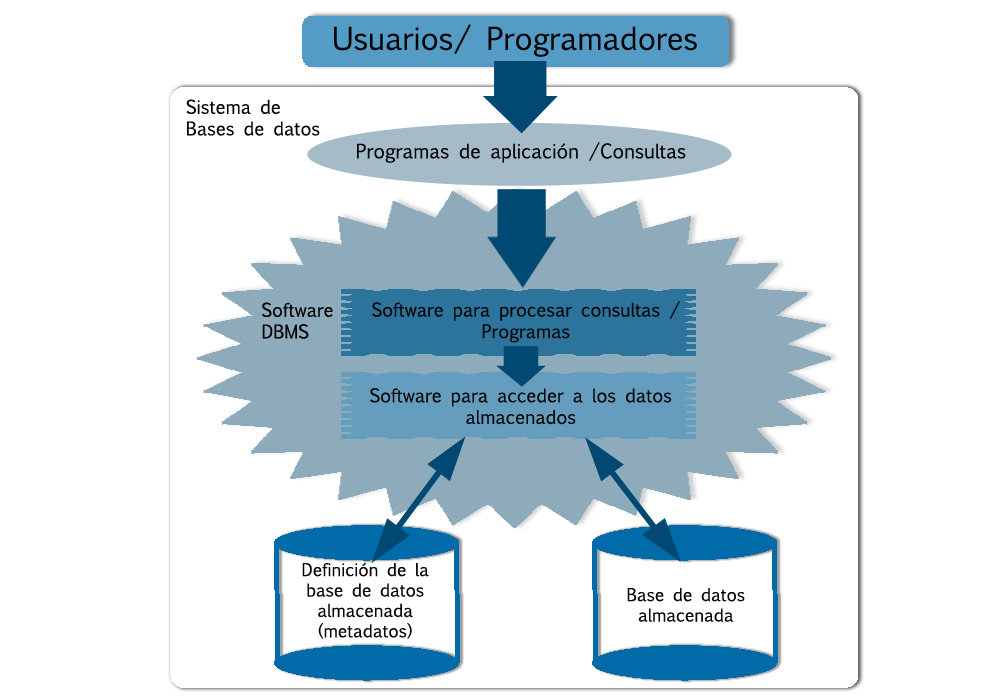
\includegraphics [scale=0.45]{capitulo1/images/figura1-1.png} \end{center}
 \caption[Entorno de un sistema de bases de datos
 simplificado]{\label{Figura 11}Entorno de un sistema de bases de datos
 simplificado \cite{navathe}}
 \end{figure}
%%%%%%%%%%%%%%%%%%%%%%%%%%%%%%%%%%%%%%%%%%%%%%%%%%%%%%%%%%%%%%%%%%
% \section{La evoluci�n del modelado de bases de datos}
% 
% \noindent Existieron dos modelos de datos antes del modelo relacional de base
% de datos, el modelo jer�rquico y modelo de red, que  
% fueron soluciones parciales de problemas interminables de como almacenar datos y c�mo 
% hacerlo eficientemente. El modelo relacional de base de datos es actualmente la mejor 
% soluci�n tanto para almacenamientos como recuperaci�n de datos.
% 
% \noindent La evoluci�n de los modelos de base de datos tuvo lugar cuando cada
% modelo de base de datos mejor� del anterior. La soluci�n inicial no fue una base de datos 
% si no que un sistema de archivos, dependiente del sistema operativo.
% Se pueden examinar archivos en el sistema de archivos del sistema operativo
% ejecutando el comando ``dir'' en DOS, un comando ``ls'' en UNIX, o buscando a trav�s del
% Explorador de Windows en Microsoft Windows. El problema que se presenta utilizando un sistema de archivos es que 
% no existe una estructura de base de datos.
% 
% \par
% 
% \noindent La figura \ref{Figura 12} muestra el proceso de evoluci�n en el tiempo
% desde los finales de 1940.
% 
% 
% %%%%%%%%%%%%%%%%%%%%%%%%%%%%%%%%%%%%%%%%%%%%%%%%%%%%%%%%%%%%%%%%%%%%%
%  \begin{figure}[H]
%  \begin{center}
%   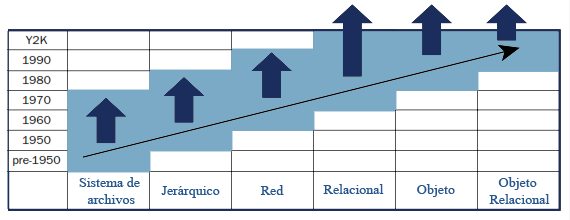
\includegraphics [scale=0.8]{capitulo1/images/figura1-2.png} \end{center}
%  \caption{\label{Figura 12}La evoluci�n de las t�cnicas de modelos de bases de datos.}
%  \end{figure}
% %%%%%%%%%%%%%%%%%%%%%%%%%%%%%%%%%%%%%%%%%%%%%%%%%%%%%%%%%%%%%%%%%%

% \subsection{Bases de datos relacionales}
% 
% \noindent Las bases de datos relacionales mejoraron en la restricci�n de la
% estructura jer�rquica, no abandonando completamente la jerarqu�a de datos, 
% como se muestra en la figura \ref{Figura 13}, en donde un tipo de empleado tiene
% muchos empleados asociados o dentro de una compa��a existen muchos departamentos.
% Cualquier tabla puede ser accedida directamente sin tener que acceder a todos los objetos padres \cite{powell}.
% 
% 
% %%%%%%%%%%%%%%%%%%%%%%%%%%%%%%%%%%%%%%%%%%%%%%%%%%%%%%%%%%%%%%%%%%%%%
%  \begin{figure}[H]
%  \begin{center}
%   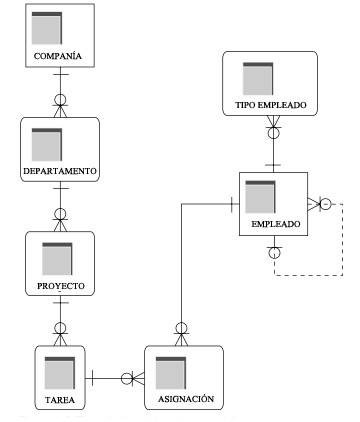
\includegraphics [scale=0.7]{capitulo1/images/figura1-51.png} \end{center}
%  \caption{\label{Figura 13}Modelo relacional}
%  \end{figure}
% %%%%%%%%%%%%%%%%%%%%%%%%%%%%%%%%%%%%%%%%%%%%%%%%%%%%%%%%%%%%%%%%%%
% 
% \par
% \noindent El modelo de datos relacional introdujo lenguajes de consulta
% de alto nivel que suministraban una alternativa a las interfaces de lenguaje de programaci�n; 
% por lo que era mucho m�s r�pido escribir consultas nuevas. La representaci�n relacional de los 
% datos se parece al ejemplo presentado en la figura \ref{Figura 14}. Los sistemas
% relacionales estaban destinados inicialmente a las mismas aplicaciones que los primitivos sistemas, pero estaban pensados para 
% ofrecer flexibilidad en el desarrollo de nuevas consultas y para reorganizar la base de datos 
% cuando cambiaran los requisitos. Su rendimiento mejor� con el desarrollo de nuevas t�cnicas de almacenamiento e 
% indexaci�n y unas t�cnicas mejores de procesamiento y optimizaci�n. Eventualmente, las bases de 
% datos relacionales se convirtieron en el tipo de sistema de bases de datos predominante para las 
% aplicaciones de bases de datos tradicionales \cite{navathe}.
% 
% 
% 
% %%%%%%%%%%%%%%%%%%%%%%%%%%%%%%%%%%%%%%%%%%%%%%%%%%%%%%%%%%%%%%%%%%%%%
%  \begin{figure}[H]
%  \begin{center}
%   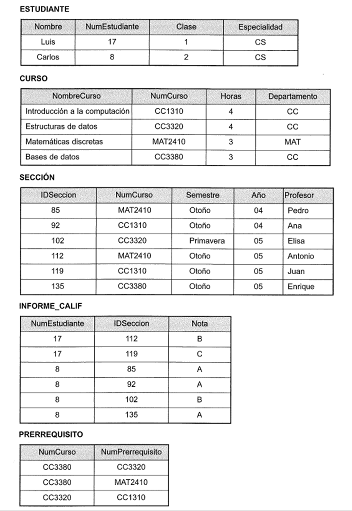
\includegraphics [scale=0.9]{capitulo1/images/figura1-5.png} \end{center}
%  \caption{\label{Figura 14}Base de datos que almacena la informaci�n de
%  estudiantes y cursos}
%  \end{figure}
% %%%%%%%%%%%%%%%%%%%%%%%%%%%%%%%%%%%%%%%%%%%%%%%%%%%%%%%%%%%%%%%%%%
% 
% 
% \subsection{Bases de datos objeto relacional}
% 
% \noindent El modelo de bases de datos objeto relacional fue creado como respuesta a las capacidades 
% conflictivas de los modelos relacionales y orientado a objetos.
% Esencialmente las capacidades que posee el modelo orientado a objetos ya se
% encuentran incluidos en las bases de datos relacionales, sin embargo las
% capacidades de una base de datos relacional no est�n incorporadas en las bases
% de datos orientadas al objeto.
% El modelo objeto relacional intenta incluir los aspectos m�s eficientes del modelo orientado a objetos en 
% la estructura del modelo relacional, con variados grados de �xito \cite{powell}.
% 
% \noindent Algunos sistemas de administraci�n de base de datos como Oracle,
% a�adieron algunas capacidades orientadas a objetos a sus productos, resultando 
% en bases de datos h�brida objeto-relacionales. El modelo objeto-relacional extiende 
% al modelo relacional agregando algunos tipos de datos complejos y m�todos. En vez 
% de atomicidad y valores simples en los atributos que requiere el modelo relacional, 
% este modelo permite atributos estructurados y tienen conjuntos de arreglos de valores. 
% Tambi�n permite m�todos y herencia. El lenguaje SQL fue extendido en 1999 para crear y 
% manipular los tipos de datos m�s complejos que soporta este modelo, como la especificaci�n 
% de tipos de datos abstractos (denominados TDA o tipos definidos por el usuario)
% \cite{navathe}. 
% 
% %%%%%%%%%%%%%%%%%%%
% 
% \subsection{Datos semi estructurados}
% 
% \noindent En palabras simples son datos sin esquema o auto descriptibles, la
% informaci�n sobre la estructura est� junto con los datos. En la actualidad es
% una necesidad integrar los datos muy estructurados con los poco estructurados.  
% La principal diferencia entre ambos es la forma de manejar los constructores 
% del esquema (nombres de atributos, relaciones y tipos de entidades, entre
% otros.).
% %En
% % el caso de los poco estructurados, la informaci�n del esquema se mezcla con los
% %  valores de los datos ya que un objeto de datos puede tener diferentes atributos 
% %  no conocidos por adelantado. Por eso, estos tipos de datos se conocen como datos auto descriptivos.
%  
%  \noindent La mayor parte de los modelos de base de datos requiere que los tipos
%  de entidades (u objetos o registros, dependiendo del modelo) posean la misma estructura. 
%  La estructura se define en el esquema y permanece sin modificaciones a menos que el 
%  administrador de la base de datos cambie dicho esquema. A diferencia, el modelo semi 
%  estructurado posibilita una colecci�n de nodos, cada uno conteniendo datos, posiblemente 
%  con diferentes esquemas. El nodo tiene informaci�n sobre la estructura de su contenido. 
%  
% %  \noindent Algunas caracter�sticas de los datos semi estructurados son:
% %  
% %  \begin{itemize}
% %    \item No existe necesariamente una diferencia entre un identificador de un
% %    campo y el valor mismo de este.
% %    \item Un atributo de un registro puede ser otro registro.
% %    \item Un registro no necesariamente tiene que tener todos sus atributos
% %    definidos. Mientras por ejemplo en una base de datos relacional un campo 
% %    debe establecerse como NULL cuando no se tiene, en un ambiente de datos semi 
% %    estructurados basta con omitir dicho atributo.   
% %  \end{itemize}
% %  \par
%  \noindent A pesar de poder representarse de distintas formas, como por ejemplo
%  documentos SGML (Standard Generalized Markup Language) y XML, actualmente la
%  mejor manera de hacerlo es a trav�s del lenguaje XML.\\
% 
% \par 
% \noindent \tn{XML} (eXtensible Markup Language)
% 
% \noindent El lenguaje XML es el est�ndar para estructurar e intercambiar datos
% por la Web, el cual se puede utilizar para suministrar informaci�n sobre la estructura y el 
% significado de ciertos componentes de los datos visualizados en una p�gina web, 
% en vez de especificar c�mo se debe visualizar la informaci�n, trabajo que realiza 
% % el lenguaje HTML. El formateo de la visualizaci�n se puede especificar por separado, 
% % por ejemplo mediante XSL (Lenguaje de hojas de estilo extensible, Extensible Stylesheet Language). 
% Recientemente, tambi�n se ha propuesto a XML como un posible modelo para el almacenamiento y la 
% recuperaci�n de datos, aunque hasta el momento s�lo se han desarrollado unos pocos sistemas de 
% bases de datos experimentales basados en XML.
% 
% \noindent Posee las siguientes caracter�sticas principales:
% 
% \begin{itemize}
%   \item \tn{Sencillo}: F�cil de aprender y de usar.
%   \item \tn{Vers�til}: Separa contenido, estructura y presentaci�n.
%    \item \tn{Abierto}: Independiente de plataformas, empresas, lenguajes de
%   programaci�n o entornos de desarrollo.
%   \item \tn{Extensible}: Se pueden definir nuevas etiquetas.
%   \item \tn{Validable}: Cada documento se puede validar frente a un esquema  o
%   definici�n de tipo de documento (\tn{DTD}), o se puede declarar bien formado.
%     \item \tn{Estructurado}: Se pueden modelar datos a cualquier nivel de
%   complejidad.
% 
% 
% \end{itemize}
%  
% % \par
% % \noindent El objeto b�sico en XML es el documento XML. En la construcci�n de un
% % documento XML se utilizan dos conceptos de estructuraci�n principales: elementos 
% % y atributos. Los atributos en XML proporcionan informaci�n adicional que
% % describe a los elementos \cite{navathe}.
% 
% % \par
% % \noindent Es posible distinguir tres tipos principales de documentos XML: 
% % 
% % \begin{itemize}
% %   \item \tn{Documentos XML centrados en los datos}: Estos documentos tienen
% %   muchos elementos de datos peque�os que respetan una estructura espec�fica y, por tanto, 
% %   pueden extraerse de una base de datos estructurada. Se formatean como documentos 
% %   XML para intercambiarlos o visualizarlos por la Web. 
% %   \item \tn{Documentos XML centrados en el documento}: Son documentos con
% %   grandes cantidades de texto, como los art�culos y los libros. En estos documentos 
% %   hay pocos o ning�n elemento de datos estructurado.
% %   \item \tn{Documentos XML h�bridos}: Estos documentos pueden tener partes que
% %   contienen datos estructurados y otras partes que son principalmente 
% %   textuales o no estructuradas.
% % \end{itemize}
% 
% 
% 
% 
% % \noindent \tn{Documentos XML bien formados}
% % 
% % \noindent Un documento XML est� bien formado s�lo
% % si existe una ra�z y todas las etiquetas de comienzo poseen su correspondiente
% % etiqueta de cerrado, con su correspondiente anidaci�n \cite{wang}. Por ejemplo,
% % el C�digo  \ref{codigo1} del documento no est� bien formado. Es posible trabajar
% % con documentos no asociados a ninguna DTD y que en consecuencia jam�s podr�n ser
% % validos. El C�digo \ref{codigo3} representa un documento que se encuentra
% % bien formado.
% % 
% % \newpage
% % 
% % %\belowcaptionskip=-10pt
% % 
% % \begin{lstlisting}[language=xml, caption={C�digo de documento XML
% % que no se encuentra bien formado}, label=codigo1] 
% % <bookcatalog>
% % <book>
% % <title>History of Interviews</ti>
% % <author>
% % <firstname>Juan</firstname>
% % <lastname>Smith</author></lastname>
% % <ISBN>99999-99999</ISBN>
% % <publisher>Oracle Press</publisher>
% % <publishyear>2003</publishyear>
% % <price type="US">10.00</price>
% % </book>
% % </bookcatalog>
% % <bookcatalog2>
% % �
% % </bookcatalog2>
% % \end{lstlisting}
% % 
% % \par 
% % \noindent Las razones por las que no es bien formado son:
% % 
% % \begin{itemize}
% %   \item Existen dos ra�ces, 'bookcatalog' y 'bookcatalog2'.
% %   \item La etiqueta <title> \ no posee su etiqueta de t�rmino correspondiente,
% %   la que ser�a </title>.
% %   \item La etiqueta de t�rmino </author> \ no se encuentra correctamente
% %   anidada, ya que la etiqueta de termino </lastname> \ est� posicionada despu�s de la
% %   </author>, en vez de ubicarse antes de ella. Los analizadores XML rechazar�n
% %   este documento sin procesamiento adicional.
% % \end{itemize}
% % 
% % 
% % 
% % 
% % \begin{lstlisting}[language=xml, caption={C�digo de documento XML
% % bien formado}, label=codigo3] 
% % <bookcatalog>
% % 	<book>
% % 		<title>History of Interviews</title>
% % 		<author>
% % 			<firstname>Juan</firstname>
% % 			<lastname>Smith</author></lastname>
% % 		</author>
% % 		<ISBN>99999-99999</ISBN>
% % 		<publisher>Oracle Press</publisher>
% % 		<publishyear>2003</publishyear>
% % 		<price type="US">10.00</price>
% % 	</book>
% % </bookcatalog>
% % \end{lstlisting}
% 
% \noindent \tn{Documentos XML V�lidos}
% \par
% \noindent Un documento XML v�lido es el que est� conformado por un esquema XML o
% definici�n de tipo de documento (\tn{DTD}), esto significa que los elementos, atributos, relacionales estructurales y secuencias
% en el documento XML son los mismos que los previamente especificados en el
% esquema XML o definici�n de tipo de documento (\tn{DTD}) \cite{wang}. Por ejemplo, el c�digo \ref{codigo2} documento
% XML es v�lido con respecto al DTD. 
% 
% \noindent En el c�digo \ref{codigo4} se representa el
% DTD, donde la declaraci�n DOCTYPE especifica el elemento ra�z, en
% este caso el elemento \ <bookcatalog>. Un elemento simple se compone de una etiqueta de
% inicio, por ejemplo, \ <title>; todo el texto ``History of Interviews'' entre
% medio de la etiqueta de inicio y la t�rmino \ </title>. Sin embargo, s�lo un 
% elemento ra�z existe en un documento XML. El elemento ra�z marca el inicio del
% documento y es considerado el padre de todos los otros elementos, los cuales se
% encuentran anidados con sus respectivas etiquetas de inicio y t�rmino. Para que
% los documentos XML sean considerados v�lidos con respecto a su DTD, el elemento
% ra�z \tn{bookcatalog} debe ser el primer elemento para empezar el cuerpo del
% documento XML.
% 
% \noindent As�, un analizador XML de validaci�n, al analizar el documento XML de
% acuerdo con las reglas especificadas en el DTD, intenta
% determinar si el documento se ajusta a la DTD (si es v�lido), lo que significa
% que todos los elementos requeridos, atributos, relaciones estructurales y
% secuencias est�n seg�n lo declarado. \\
% 
% 
% 
% 
% \begin{lstlisting}[language=xml, caption={C�digo de documento XML
% validamente formado}, label=codigo2] 
% <bookcatalog>
% <book>
% <title>History of Interviews</title>
% <author>
% <firstname>Juan</firstname>
% <lastname>Smith</lastname>
% </author>
% <ISBN>99999-99999</ISBN>
% <publisher>Oracle Press</publisher>
% <publishyear>2003</publishyear>
% <price type="US">10.00</price>
% </book>
% </bookcatalog>
% 
% \end{lstlisting}
% 
% 
% \newpage
% 
% \begin{lstlisting}[language=xml, caption={C�digo DTD}, label=codigo4] 
% <!-- DTD bookcatalog may have a number of book entries -->
% <!DOCTYPE bookcatalog [
% <!ELEMENT bookcatalog (book)*>
% <!-- Each book element has a title, 1 or more authors, etc. -->
% <!ELEMENT book (title, author+, ISBN, publisher, publishyear, price)>
% <!ELEMENT title (#PCDATA)>
% <!ELEMENT author (firstname, lastname)>
% <!ELEMENT firstname (#PCDATA)>
% <!ELEMENT lastname (#PCDATA)>
% <!ELEMENT ISBN (#PCDATA)>
% <!ELEMENT publisher (#PCDATA)>
% <!ELEMENT publishyear (#PCDATA)>
% <!ELEMENT price (#PCDATA)>
% <!ATTLIST price type (US | CAN | UK | EURO) #REQUIRED>
% ]>
% 
% \end{lstlisting}
% 
% \noindent Existen dos caminos primarios para almacenar XML contenido en una base
% de datos relacional:
% 
% \begin{itemize}
%   \item \tn{Estructurado}: El almacenamiento estructurado descompone el
%   contenido del documento XML dentro de un juego de objetos. Un beneficio es que los datos pueden ser
% accesados por aplicaciones que entiendan solamente base de datos relacionales.
%   \item \tn{No estructurado}: Con el almacenamiento no estrucurado, el documento
%   XML es almacenado de forma nativa como un character large object (CLOB) dentro de la base de
% datos.
% \end{itemize}


\section{Problema a resolver}

\noindent %Existen falencias en ciertas gu�as, por ende es preciso determinar
%cual es la mejor estrategia de base de datos a utilizar y para eso se realizar�
%esta comparaci�n. 
El estudio que se realizar� estar� centrado 
en la implementaci�n de un caso de estudio propuesto en una base de datos
relacional, una base de datos objeto relacional y el manejo de datos semi
estructurados con XML, con el fin de generar una gu�a para seleccionar el tipo
de base de datos m�s adecuada seg�n la aplicaci�n a
desarrollar y de esta forma tener claro las ventajas y desventajas de cada
implementaci�n, por lo que se realizar�n pruebas en cada una de
�stas, con el prop�sito de analizar los resultados obtenidos.

\section{Justificaci�n}


\noindent La realizaci�n de esta investigaci�n tiene como prop�sito adquirir la
capacidad de examinar los conceptos de bases de datos relacional, bases de datos
objeto relacional y datos semi estructurados, sin embargo, implica mucho m�s que
la utilizaci�n de dichos conceptos, ya que consiste en poder seleccionar el
modelo de datos m�s apropiado a implementar en un sistema y / o aplicaci�n en
particular. Y de esta forma lograr responder la pregunta �Por qu� este modelo
de base de datos es m�s adecuado para el desarrollo de mi software?

\noindent Es sumamente importante para los desarrolladores sacarle provecho a
las capacidades que se han ido incorporando a los servidores de base de datos,
ya que es relevante modelar seg�n las aptitudes de las bases de datos, 
puesto que tienen m�s sem�ntica y los datos no est�n fragmentados como en una base de datos 
relacional pura, por lo que no se restringe a la primera forma normal y a causa de esto 
pueden existir atributos no at�micos.

\noindent Es v�lido acotar que la capa de persistencia de datos del software que
se desea desarrollar, puede variar seg�n la implementaci�n seleccionada de
la gu�a a generar mediante los resultados obtenidos en esta investigaci�n.

\noindent Cabe mencionar que el obtener resultados efectivos permitir� cooperar
con documentaci�n y casos de estudio para la asignatura de base de datos.

\noindent A modo personal del tesista, se busca adquirir experiencia y
conocimientos de avanzada para el desarrollo profesional en el �rea de base de datos, 
espec�ficamente en las �reas relacionadas con los sistemas de administraci�n de base de datos, 
bases de datos objeto relacional y datos semi estructurados como XML. As� mismo, adquirir un 
mayor nivel de conocimiento en las capacidades que poseen los servidores de base de datos, 
como es la implementaci�n de procedimientos almacenados utilizando lenguajes de programaci�n 
sin tener que implementar fuera del servidor del sistema de administraci�n de base de datos.


\section{Objetivos}

\noindent \tn{Objetivo general}

\noindent Evaluar y comparar la implementaci�n de una base de datos relacional
con respecto a una base de datos objeto relacional y datos semi estructurados 
en el sistema de administraci�n de base de datos Oracle, utilizando las 
funciones disponibles en el servidor del SABD, con el fin de generar una gu�a que en base a 
criterios claros permita determinar cu�l es el tipo de base de datos m�s 
adecuada a utilizar bajo ciertas caracter�sticas.\\

\noindent \tn{Objetivos Espec�ficos}

\begin{itemize}
\item Estudiar, seleccionar y utilizar funciones del sistema de administraci�n
de base de datos relacional Oracle 11G, que permitan la implementaci�n de bases
de datos objeto relacional y XML.

\item Comprender los m�ltiples m�todos de implementaci�n de los modelos
mencionados con anterioridad para ser capaz de seleccionar adecuadamente entre
ellos seg�n la aplicaci�n a desarrollar.


\item Dise�ar el caso de estudio para luego implementarlo con
Oracle 11G en una base de datos relacional, objeto relacional y datos semi
estructurados como XML.


\item Definir criterios de comparaci�n para las implementaciones tales como: facilidad de modelamiento, complejidad de aprendizaje 
por parte del desarrollador y/o DBA, entre otros.

\item Realizar un an�lisis de resultados, en donde se compare cada una de las
implementaciones, con el fin de
estructurar una gu�a con los beneficios y desventajas dependiendo de la
aplicaci�n a desarrollar, seg�n los criterios de comparaci�n.


\end{itemize}


\section{Descripci�n}

\noindent El problema a dar soluci�n es generar la capacidad de comprender los
m�ltiples conceptos y m�todos de implementaci�n relacionados con bases de datos
relacionales, objeto relacional y datos semi estructurados como XML y poder
justificar la selecci�n del modelo m�s adecuado para diferentes aplicaciones. 
Para lograr este objetivo se pretende implementar
dichos modelos s�lo utilizando las caracter�sticas
nativas presentes en el servidor del SABD Oracle 11G, con el fin de crear una
gu�a para seleccionar el tipo de base de datos m�s adecuada seg�n la aplicaci�n a desarrollar.

\noindent La primera etapa contempla hacer una investigaci�n
exhaustiva de los sistemas de administraci�n de base de datos que tengan soporte para implementar bases de datos objeto relacional y datos semi 
estructurados como XML. A continuaci�n en su segunda etapa, se dise�ar� un caso de 
estudio, el cual ser� implementado en una base de datos relacional en Oracle. \\
\noindent Posteriormente en la tercera etapa, se implementar� el caso de estudio
en una base de datos objeto relacional y datos semi estructurados como XML. En la cuarta etapa, se 
realizar�n pruebas con una cierta cantidad de datos en cada versi�n, para luego
analizar los resultados obtenidos bajo ciertos criterios que ser�n definidos.
Por �ltimo se generar� un documento gu�a con la informaci�n recolectada.


\section{Resultados esperados}

\noindent Se obtendr�n tres productos finales:

\begin{itemize}
  \item \tn{Documento con marco te�rico}: El documento de memoria contendr�
  todo el marco te�rico asociado a la creaci�n de una base de datos relacional,
  base de datos objeto relacional, el manejo de datos semi estructurados como
  XML desde el punto de vista del intercambio de informaci�n.
  \item \tn{Caso de estudio implementado}: Implementar un caso de estudio en una
  base de datos relacional, objeto relacional y datos semi estructurados como XML en Oracle.
  \item \tn{Comparaci�n de implementaciones}: Generar un documento que indique
  las ventajas y desventajas de cada implementaci�n considerando facilidad de modelamiento, facilidad de aprendizaje por parte del desarrollador, entre otros.
  Y con esto poder tomar mejores decisiones en cuanto a la elecci�n del tipo de
  SABD a seleccionar y el manejo de datos semi estructurados dependiendo del
  tipo de aplicaciones a desarrollar.
\end{itemize}


\section{Metodolog�a}

\noindent A continuaci�n se describir� de forma cronol�gica la metodolog�a que
se realizar� en esta investigaci�n:

\begin{itemize}
\item \tn{Metodolog�a de investigaci�n}

\noindent En un inicio para lograr establecer el estado del arte del tema de
investigaci�n, se har� una revisi�n de la literatura sobre los diversos 
SABD con la capacidad de implementar bases de
datos objeto relacional y XML.
Para luego explorar en profundidad  los m�todos y / o funciones imprescindibles para
crear cada implementaci�n en Oracle 11G.

\item \tn{Metodolog�a de dise�o de modelo de datos}

\noindent Para el dise�o del caso de estudio que se implementar� en cada base de
datos se aplicar�n los m�todos adquiridos en la asignatura. A continuaci�n se
detalla cada paso a realizar:

\begin{itemize}
  \item Dise�ar un caso de estudio.
  \item Modelar la base de datos relacional y hacer la documentaci�n asociada
  incluyendo el modelo relacional.
  \item Modelar la base de datos objeto relacional y documentar utilizando UML.
\end{itemize}

\item \tn{Metodolog�a de implementaci�n y comparaci�n}


\begin{itemize}  
  
  \item Implementaci�n del caso de estudio utilizando una base de datos
  relacional pura.
  
  \item Implementaci�n del caso de estudio utilizando una base de datos objeto
  relacional y datos semi  estructurados como  XML, disponibles en el
  SABD Oracle.
  
  \end{itemize}
  
\noindent Primero se definir�n criterios para realizar la
comparaci�n, estos pueden ser:

\begin{itemize}
 % \item Desempe�o en consultas.
  %dise�adas para medir tiempos de respuesta. Este tipo de prueba ayudar� a
  %medir y conocer la velocidad que tiene el SABD durante la ejecuci�n de
  %cada una de las pruebas.
  \item Facilidad de modelamiento.
  \item Complejidad de aprendizaje por parte del desarrollador y/o DBA.
\item Utilizaci�n de recursos.
\end{itemize}

\noindent Procedimientos iniciales para la realizaci�n de las comparaciones: 

\begin{itemize}
  \item Ingreso de datos.
  \item Consulta de datos.
  \item Eliminaci�n de datos.
  \item Actualizaci�n de datos.
  
\end{itemize}

  
\noindent Luego de realizar las comparaciones se proceder� a estudiar 
y analizar los resultados obtenidos para generar la gu�a, en donde se detallen 
los beneficios y desventajas de cada implementaci�n de acuerdo al tipo de 
aplicaci�n que se desea desarrollar.  

\end{itemize}

\section{Recursos necesarios}

\par \noindent \tn{Hardware}

\begin{itemize}
  \item Servidores del DISC.
  \item Laptop personal con las siguientes caracter�sticas.
  \begin{itemize}
    \item Marca: Dell
    \item Modelo: XPS 15
    \item Procesador: Intel \textregistered  \ Core \texttrademark \ i7 CPU Q740
    @1.73 GHz
    \item Memoria Ram: 8 GB.
    \end{itemize} 
\end{itemize}

\par \noindent \tn{Software}

\begin{itemize}
  \item \tn{Sistema de administraci�n de bases de datos}: Oracle 11g Enterprise
  Edition.
  \item \tn{Software de modelado}: Dia.
  \item \tn{Cliente base de datos}: Oracle Sql*Plus, Oralce Sql Developer.
  \item \tn{Sistemas operativos a utilizar}: GNU/Linux / Windows.
\end{itemize}


\par \noindent \tn{Recursos Humanos}

\begin{itemize}
  \item Alumno: Ingeborg Mu�oz Carnot.
  \item Profesor Gu�a: Lotero Telgie Bendek.
  \item Profesor Gu�a: Luis Lobos Flores.
\end{itemize}
 \chapter{MARCO TE�RICO} \label{capitulo2}

\par
\noindent Este cap�tulo habla sobre c�mo ha evolucionado el
modelado de bases de datos a lo largo de la historia y detalla los conceptos de
datos semi estructurados y XML. Adem�s presenta algunos motores de bases de
datos que poseen soporte objeto relacional, en donde se especifican los m�todos 
principales de utilizaci�n de tipos y XML. Se enfatiza en
especial al sistema de administraci�n de base de datos Oracle Database 11g, ya
que es el motor elegido para implementar el caso de estudio que se definir�,
este SGDB posee las ediciones:
Oracle Database 11g Express Edition, Standar Edition y
Enterprise Edition.
\noindent La edici�n a evaluar en la presente memoria ser� Oracle Database 11g
Enterprise Edition, ya que con �sta es posible la gesti�n de la informaci�n de
forma eficiente, confiable y segura en aplicaciones transaccionales
indispensables, almacenes de datos con elevado tr�fico de consultas \cite{ora}.



\section{La evoluci�n del modelado de bases de datos}
\subsection{Generalidades}

\par \noindent Los modelos de datos son medios formales para representar los datos asociados a una situaci�n real 
y para manipular tal representaci�n. Las componentes de todo modelo de datos son las siguientes: 

\begin{itemize}
  \item Las estructuras b�sicas son los elementos b�sicos o tipos de objetos que conforman el 
modelo.
\item Las reglas que es el conjunto de lineamientos que expresan las propiedades est�ticas del 
modelo. Ellas son:
	\begin{itemize}
	  \item Las reglas de formaci�n 
	\item Las restricciones
	  \end{itemize}
\item Los operadores que permiten cambiar el estado de una base de datos modificando su 
contenido. Ellos est�n asociados a las propiedades din�micas de los elementos.
\end{itemize}

\par \noindent Los modelos de datos se pueden clasificar en modelos de alto
nivel o sem�nticos y modelos de bajo nivel o b�sicos:

\begin{itemize}
  \item \tn{Los modelos sem�nticos} capturan un mayor significado de los datos e
  intentan representar la estructura real de los datos independientemente de las caracter�sticas de almacenamiento, es decir 
ellos est�n orientados a las aplicaciones. Existen, hoy en d�a, numerosos y muy variados modelos 
sem�nticos, entre ellos se encuentran: el modelo Entidad-Relaci�n, el 
modelo Entidad-Relaci�n-Extendido (ERE) y el modelo IFO.
\item \tn{Los modelos b�sicos} constituyen el grupo de modelos que han sido
dise�ados orient�ndose al computador, sobre ellos se han desarrollado la mayor�a de los SGBD. Ellos son: el modelo 
jer�rquico, el modelo redes, el modelo relacional, el modelo orientado por
objetos y el objeto relacional. 

\end{itemize}


\par \noindent Muchos modelos sem�nticos han sido propuestos, pero pocos de ellos han atra�do el inter�s de los 
desarrolladores de sistemas de base de datos, esto tal vez es debido a la complejidad de tales 
modelos y a su dificultad para ser plasmados con los modelos b�sicos actuales. La mayor�a de los 
conceptos del modelado sem�ntico de datos han sido muy bien representados en el
modelo ERE, el cual goza de gran prestigio y popularidad en el ambiente comercial, jugando un rol muy importante 
en la mayor�a de las herramientas CASE (Computer Aided Software Engineering).

\par \noindent Existieron dos modelos de datos antes del modelo relacional de
base de datos, el modelo jer�rquico y modelo de red, que  
fueron soluciones parciales de problemas interminables de como almacenar datos y c�mo 
hacerlo eficientemente. El modelo relacional de base de datos es actualmente la mejor 
soluci�n tanto para almacenamientos como recuperaci�n de datos.

\noindent La evoluci�n de los modelos de base de datos tuvo lugar cuando cada
modelo de base de datos mejor� del anterior. La soluci�n inicial no fue una base de datos 
si no que un sistema de archivos, dependiente del sistema operativo.
Se pueden examinar archivos en el sistema de archivos del sistema operativo
ejecutando el comando ``dir'' en DOS, un comando ``ls'' en UNIX, o buscando a trav�s del
Explorador de Windows en Microsoft Windows. El problema que se presenta utilizando un sistema de archivos es que 
no existe una estructura de base de datos.

\par

\noindent La figura \ref{Figura 12} muestra el proceso de evoluci�n en el tiempo
desde los finales de 1940.


%%%%%%%%%%%%%%%%%%%%%%%%%%%%%%%%%%%%%%%%%%%%%%%%%%%%%%%%%%%%%%%%%%%%%
 \begin{figure}[H]
 \begin{center}
  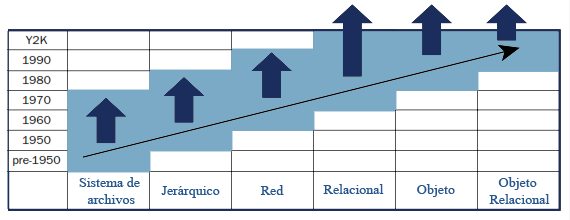
\includegraphics [scale=0.535]{capitulo1/images/figura1-2.png} \end{center}
 \caption[La evoluci�n de las t�cnicas de modelos de bases de
 datos]{\label{Figura 12}La evoluci�n de las t�cnicas de modelos de bases de
 datos \cite{powell}}
 \end{figure}
%%%%%%%%%%%%%%%%%%%%%%%%%%%%%%%%%%%%%%%%%%%%%%%%%%%%%%%%%%%%%%%%%%


\subsection{Sistema de archivos}

\noindent El uso de un sistema de archivo como modelo de base de datos implica
no aplicar t�cnicas de modelado y que la base de datos es almacenada en un archivo 
plano en un sistema de archivos, utilizando la estructura del sistema operativo.
\par \noindent Cualquier b�squeda de datos a trav�s de archivos planos debe ser
expl�citamente programada. La ventaja de diferentes modelos de bases de datos es 
que proporcionan algo de esta programaci�n. Para una base de datos de sistema de 
archivos, los datos pueden ser almacenados en archivos individuales o en m�ltiples 
archivos. Similar a buscar a trav�s de archivos planos, cualquier relaci�n y
validaci�n entre diferentes archivos planos tendr�an que ser programadas y probablemente con una capacidad limitada.

\subsection{Modelo jer�rquico de base de datos}

\noindent El modelo jer�rquico de base de datos fue desarrollado como una
soluci�n a las necesidades inmediatas de aplicaciones reales a mediados de los 60s. 
El sistema m�s antiguo e importante de base de datos jer�rquico es IMS de IBM y fue 
desarrollado para organizar y almacenar informaci�n necesaria para el proyecto de 
alunizaje del Apolo. IBM y la aviaci�n norteamericana trabajaron juntos para producir 
la primera versi�n de IMS en 1968. Las versiones posteriores de IMS fueron
dise�adas para usarse con dispositivos de cintas magn�ticas, pero los posteriores discos magn�ticos 
se convirtieron en el est�ndar. IMS r�pidamente se convirti� en el sistema de base de datos 
jer�rquico dominante en el mercado y fue por muchos a�os el DBMS m�s ampliamente usado, hasta 
que fue remplazado por los sistemas relacionales. Muchas mejoras fueron hechas a IMS despu�s 
del 68, resultando en nuevas versiones que obten�an ventajas de las mejoras en hardware y software, 
proporcionando nuevas caracter�sticas como comunicaci�n de datos y m�ximo desempe�o. IMS era capaz de 
procesar grandes cantidades de datos de modo eficiente. Usaba una estructura de �rbol familiar para 
los programadores acostumbrados a trabajar con archivos. La estructura l�gica en la que se sustenta 
es el �rbol, el cual se compone de un nodo ra�z y varios nodos sucesores, ordenados jer�rquicamente, 
como se observa en la figura \ref{Figura 12.1}. Cada nodo representa una entidad
(tipo de registro) y las relaciones entre entidades son las conexiones entre los nodos. El nodo superior es el 
nodo padre y los inferiores 
son los nodos hijos. Las conexiones entre archivos no dependen de la informaci�n contenida en ellos, 
se definen al inicio y son fijos (punteros). Las interrelaciones entre registros permiten que un padre 
tenga muchos hijos, pero un hijo s�lo puede tener un padre. Los datos se representan como estructuras de 
�rbol y el �rbol representa la jerarqu�a de registros de datos. La navegaci�n es top-down.

%%%%%%%%%%%%%%%%%%%%%%%%%%%%%%%%%%%%%%%%%%%%%%%%%%%%%%%%%%%%%%%%%%%%%
 \begin{figure}[H]
 \begin{center}
  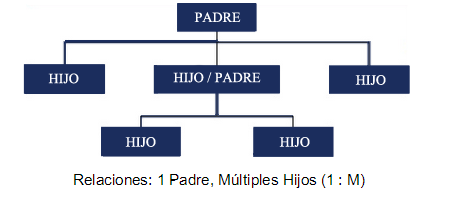
\includegraphics [scale=1]{capitulo2/images/figura1-3.png} \end{center}
 \caption{\label{Figura 12.1}Relaciones modelo jer�rquico de bases de datos}
 \end{figure}
%%%%%%%%%%%%%%%%%%%%%%%%%%%%%%%%%%%%%%%%%%%%%%%%%%%%%%%%%%%%%%%%%%

\par \noindent Desventajas:

\begin{itemize}
  \item No modela sencillamente las relaciones Muchos a Muchos.
  \item Genera anomal�as de inserci�n.
  \item Genera anomal�as de borrado.
  \item Genera anomal�as de actualizaci�n.
  \item Se pueden dar consultas inconsistentes.
\end{itemize}

\subsection{Modelo de red de base de datos}

\par \noindent El modelo de base de datos de red es esencialmente un
refinamiento del modelo jer�rquico. El modelo de red permite a las 
tablas hijas tener m�s de un padre, por lo tanto creando a una estructura de 
tabla como red. M�ltiples tablas padres para cada hijo permite relacionales de N a N (muchos es a muchos), 
en adici�n a las relacionales de 1 a N (1 a muchos). En un ejemplo de modelo de red mostrado en la 
figura \ref{Figura 12.2}, existe una relaci�n N a N entre empleados y tareas. En
otras palabras.
Un empleado puede ser asignado a muchas tareas, y una tarea puede ser asignada a diferentes empleados. Por lo tanto, muchos 
empleados tienen muchas tareas y vice versa \cite{powell}.

\par \noindent La figura \ref{Figura 12.2} muestra como los administradores
pueden ser parte de departamentos y compa��as. En otras palabras, el modelo de red est� 
tomando en cuenta que no s�lo cada departamento dentro de una empresa tiene un administrador, 
sino que tambi�n cada compa��a tiene un administrador general (en la vida real, un jefe ejecutivo o CEO). 
La figura \ref{Figura 12.2} adem�s muestra la incorporaci�n de tipos de tablas
donde los empleados puede ser definidos de diferentes tipos (tal como tiempo
completo, part-time, entre otros.). Lo m�s importante de notar es la nueva tabla
``Asignaciones'' la cual permite asignar tareas a los empleados. La creaci�n de
la tabla ``Asignaciones'' es el resultado directo de la adici�n de la capacidad de padres m�ltiples entre los modelos jer�rquicos y de red. Como ya se se�al�, la relaci�n entre las tablas empleados y tareas es de N a N, donde 
cada empleado puede ser asignado a m�ltiples tareas y cada tarea puede ser asignada a m�ltiples empleados. 
La tabla asignaci�n resuelve el problema de la relaci�n N a N, permitiendo una definici�n �nica para la 
combinaci�n de empleado y tarea. Sin esa definici�n �nica, encontrar una
asignaci�n ser�a imposible \cite{powell}.

%%%%%%%%%%%%%%%%%%%%%%%%%%%%%%%%%%%%%%%%%%%%%%%%%%%%%%%%%%%%%%%%%%%%%
 \begin{figure}[H]
 \begin{center}
  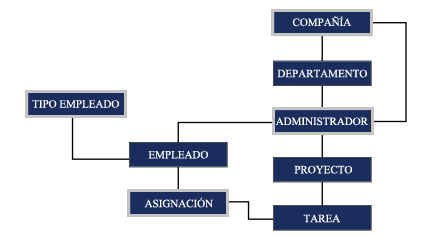
\includegraphics [scale=0.8]{capitulo2/images/figura1-4.png} \end{center}
 \caption[Modelo de red de base de datos]{\label{Figura 12.2}Modelo de red de
 base de datos \cite{powell}}
 \end{figure}
%%%%%%%%%%%%%%%%%%%%%%%%%%%%%%%%%%%%%%%%%%%%%%%%%%%%%%%%%%%%%%%%%%

\par \noindent Desventajas:

\begin{itemize}
  \item Resulta dif�cil definir nuevas relaciones.
  \item Es complicado darle mantenimiento, ya que cualquier cambio en la
  estructura requiere una descarga de los datos.
  \item Representa desperdicio de recursos.
  \item Genera anomal�as de inserci�n.
  \item Genera anomal�as de borrado.
\end{itemize}

\subsection{Bases de datos relacionales}

\noindent Las bases de datos relacionales mejoraron en la restricci�n de la
estructura jer�rquica, no abandonando completamente la jerarqu�a de datos, 
como se muestra en la figura \ref{Figura 13}, en donde un tipo de empleado tiene
muchos empleados asociados o dentro de una compa��a existen muchos departamentos.
Cualquier tabla puede ser accedida directamente sin tener que acceder a todos los objetos padres \cite{powell}.


%%%%%%%%%%%%%%%%%%%%%%%%%%%%%%%%%%%%%%%%%%%%%%%%%%%%%%%%%%%%%%%%%%%%%
 \begin{figure}[H]
 \begin{center}
  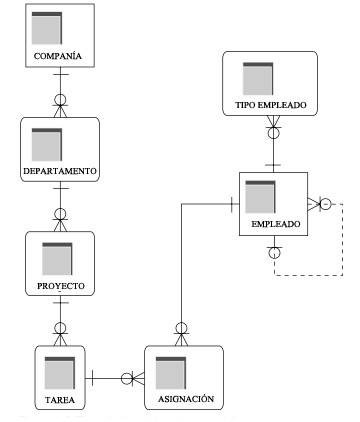
\includegraphics [scale=0.68]{capitulo1/images/figura1-51.png} \end{center}
 \caption[Modelo relacional]{\label{Figura 13}Modelo relacional \cite{powell}}
 \end{figure}
%%%%%%%%%%%%%%%%%%%%%%%%%%%%%%%%%%%%%%%%%%%%%%%%%%%%%%%%%%%%%%%%%%

\par
\noindent El modelo de datos relacional introdujo lenguajes de consulta
de alto nivel que suministraban una alternativa a las interfaces de lenguaje de programaci�n; 
por lo que era mucho m�s r�pido escribir consultas nuevas. La representaci�n relacional de los 
datos se parece al ejemplo presentado en la figura \ref{Figura 14}. Los sistemas
relacionales estaban destinados inicialmente a las mismas aplicaciones que los primitivos sistemas, pero estaban pensados para 
ofrecer flexibilidad en el desarrollo de nuevas consultas y para reorganizar la base de datos 
cuando cambiaran los requisitos. Su rendimiento mejor� con el desarrollo de nuevas t�cnicas de almacenamiento e 
indexaci�n y unas t�cnicas mejores de procesamiento y optimizaci�n. Eventualmente, las bases de 
datos relacionales se convirtieron en el tipo de sistema de bases de datos predominante para las 
aplicaciones de bases de datos tradicionales \cite{navathe}.




\par \noindent Debilidades de los SABD Relacionales:

\begin{itemize}
  \item \tn{Mal soporte de las transacciones de larga duraci�n}: Suelen ser
  mucho m�s comunes para objetos m�s complejos.
  \item \tn{Estructura de datos que no permite heterogeneidad}: Este modelo
  admite homogeneidad vertical y horizontal. Cada tupla posee los mismos
  atributos. Los valores de una columna tienen que pertenecer al mismo dominio.
  La intersecci�n de fila y columna debe ser un valor at�mico.
  \item \tn{Pocas facilidades para navegar por los datos}: Acceso asociativo
  basado en contenido y no basado en el movimiento entre registros individuales.
  \item \tn{Operaciones restringidas}: Se tienen operaciones orientadas a
  tuplas, operaciones que proporciona SQL, pero lamentablemente SQL no tolera definir
   nuevas operaciones.
   \item \tn{Representaci�n pobre de entidades consideradas del ``mundo real''}:
   La fragmentaci�n de una entidad del ``mundo real'' en varias relaciones es
   ineficiente ya que lleva a muchos ``joins'' en el procesamiento de
   consultas.
   \item \tn{Manejo complicado de consultas recursivas}: Es complicado manejar consultas sobre relaciones que una relaci�n  tiene consigo misma
   (directa o indirectamente).
\end{itemize}

%%%%%%%%%%%%%%%%%%%%%%%%%%%%%%%%%%%%%%%%%%%%%%%%%%%%%%%%%%%%%%%%%%%%%
 \begin{figure}[H]
 \begin{center}
  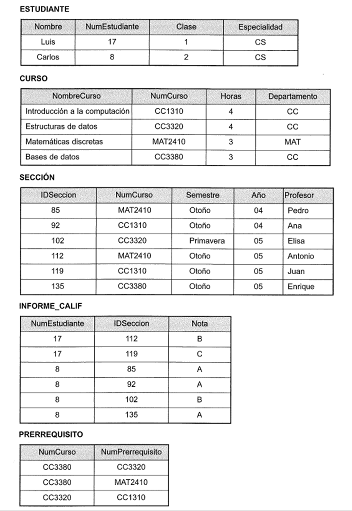
\includegraphics [scale=1]{capitulo1/images/figura1-5.png} \end{center}
 \caption[Base de datos que almacena estudiantes y cursos]{\label{Figura 14}Base de datos que almacena la informaci�n de
 estudiantes y cursos \cite{navathe}}
 \end{figure}
%%%%%%%%%%%%%%%%%%%%%%%%%%%%%%%%%%%%%%%%%%%%%%%%%%%%%%%%%%%%%%%%

\subsection{Bases de datos orientadas al objeto}

%%%%%%%%%%%%%%%%%%%%%%%%%%%%%%%%%%%%%%%%%%%%%%%%%%%%%%%%%%%%%%%%%%%%%
 \begin{figure}[H]
 \begin{center}
  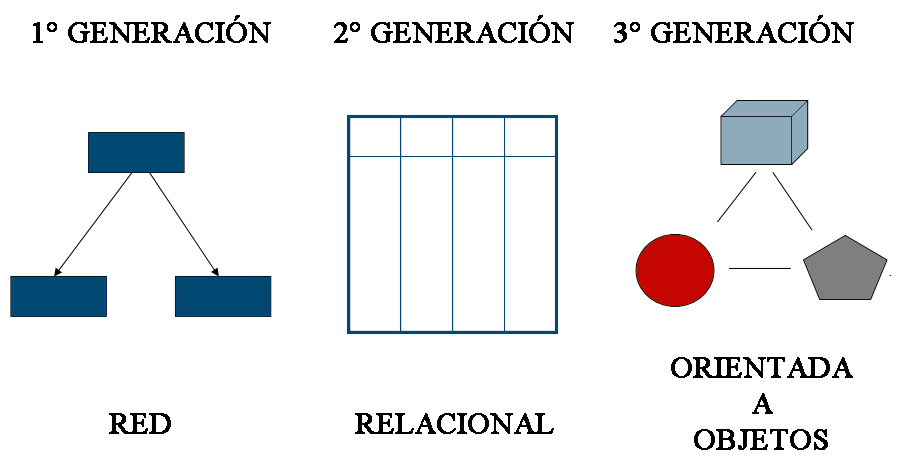
\includegraphics [scale=0.45]{capitulo2/images/generacionesbd.png}
  \end{center}
 \caption{\label{Figura 20}Tercera generaci�n de bases de datos}
 \end{figure}
%%%%%%%%%%%%%%%%%%%%%%%%%%%%%%%%%%%%%%%%%%%%%%%%%%%%%%%%%%%%%%%%%%


\noindent Una base de datos orientada a objetos pertenece a la tercera
generaci�n de bases de datos, ver figura \ref{Figura 20}, la cual proporciona a
los datos una estructura tridimensional, donde cualquier item en una base de
datos puede ser recuperado desde cualquier punto de una forma r�pida. Considerando que el modelo
relacional se presta para la recuperaci�n de grupos de registros en dos
dimensiones, el modelo orientado al objeto es eficiente para encontrar items
�nicos. Por consiguiente, este modelo se desempe�a pobremente cuando se desea
recuperar m�s de un item, en lo que el modelo relacional es muy competente.
\par
\noindent Este tipo de base de datos resuelve algunas de las complejidades m�s
ocultas de las bases de datos relacionales. La figura \ref{Figura 21} muestra un
ejemplo de la estructura de un modelo orientado a objetos y su equivalencia en
el relacional se encuentra en la figura \ref{Figura 13}. La asignaci�n de tareas a los empleados fue manejada utilizando la inclusi�n de colecciones (listas) en manager,
empleado y las especializaciones de la clase empleado. Adem�s se debe notar que
los diferentes tipos de empleados fueron manejados utilizado especializaci�n.
\par \noindent Otro beneficio de este modelo es la habilidad inherente de
gestionar y atender aplicaciones y modelos de bases de datos extremadamente
complejos. Esto es debido a un principio b�sico de la metodolog�a de la
orientaci�n a objetos, por lo que los elementos altamente complejos pueden
descomponerse en sus partes m�s elementales, lo que permite su acceso expl�cito,
as� como tambi�n su ejecuci�n a trav�s de esas partes b�sicas. En otras
palabras, si se tiene claro c�mo funcionan las peque�as piezas individualmente,
se puede visualizar el problema completo, que es una combinaci�n de un peque�o
n�mero de piezas, piezas constituyentes mucho m�s simples \cite{powell}.

\par \noindent Una discusi�n recurrente, dice que uno de los
puntos de fricci�n entre las aplicaciones orientadas al objeto y las bases de
datos relacionales es el rendimiento del proceso de mapeo entre los tipos
estructurales: Objeto y relacional. La estructura de ambos es completamente
diferente.



%%%%%%%%%%%%%%%%%%%%%%%%%%%%%%%%%%%%%%%%%%%%%%%%%%%%%%%%%%%%%%%%%%%%%
 \begin{figure}[H]
 \begin{center}
  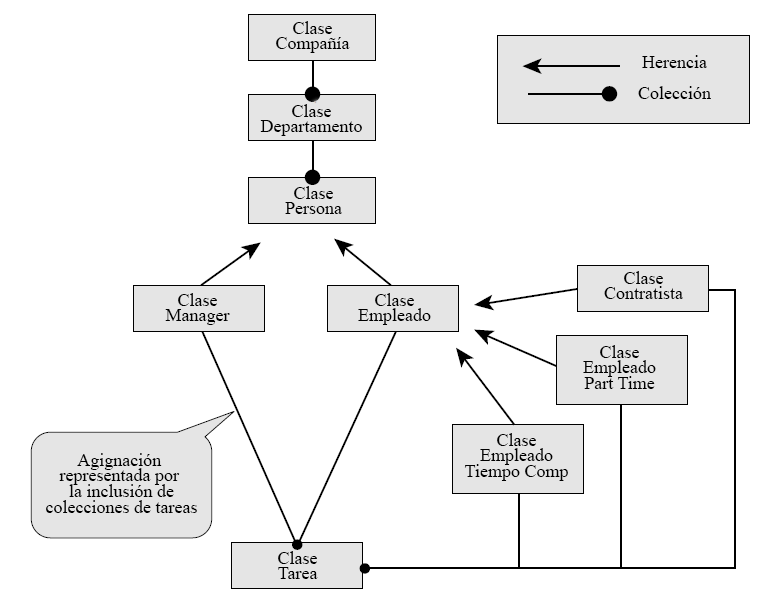
\includegraphics [scale=0.385]{capitulo2/images/orientado.png} \end{center}
 \caption[Modelo de bases de datos orientado a objetos]{\label{Figura 21}Modelo
 de bases de datos orientado a objetos
 \cite{powell}}
 \end{figure}
%%%%%%%%%%%%%%%%%%%%%%%%%%%%%%%%%%%%%%%%%%%%%%%%%%%%%%%%%%%%%%%%%%

\subsubsection{Objeto}
\noindent Es una entidad del mundo real percibida en el sistema. En palabras
t�cnicas se describe como por sus propiedades, mejor conocidas como
\ti{atributos} y los \ti{m�todos} que puede facilitar. El estado de un objeto se
determina por los valores que posean sus atributos, valores que siempre han de
satisfacer las restricciones implantadas sobre ellos. En la figura \ref{Figura
22} se muestra un ejemplo de objeto. Los m�todos definen el comportamiento del
objeto.

%%%%%%%%%%%%%%%%%%%%%%%%%%%%%%%%%%%%%%%%%%%%%%%%%%%%%%%%%%%%%%%%%%%%%
 \begin{figure}[H]
 \begin{center}
  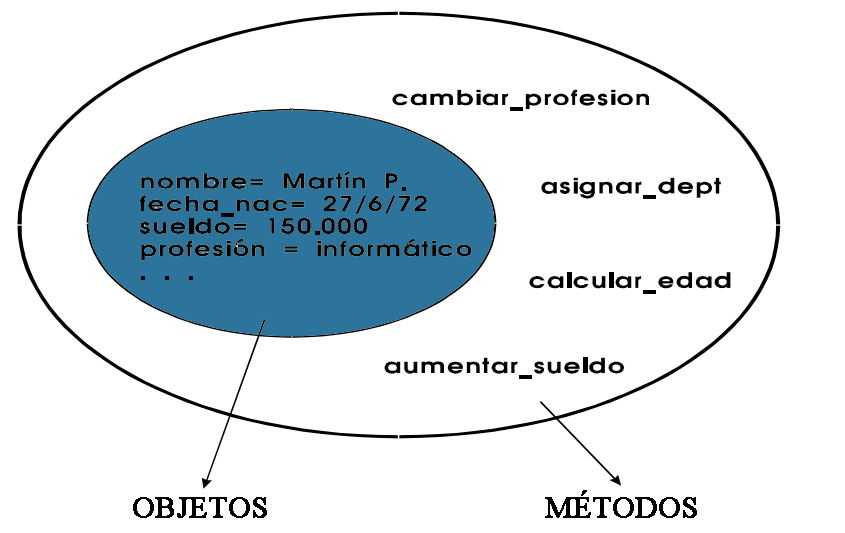
\includegraphics [scale=0.5]{capitulo2/images/objeto.png} \end{center}
 \caption{\label{Figura 22}Ejemplo de objeto}
 \end{figure}
%%%%%%%%%%%%%%%%%%%%%%%%%%%%%%%%%%%%%%%%%%%%%%%%%%%%%%%%%%%%%%%%%%

\par \noindent \tn{Abtracci�n}

\noindent Es el proceso que identifica los aspectos primordiales pero ignora el
resto. Conlleva centrarse en qu� hace y qu� es un objeto antes de pensar en c�mo
implementarlo.
\noindent Posee dos aspectos elementales:
\begin{itemize}
  \item \tn{Encapsulaci�n}: Un objeto contiene la estructura de los datos y su
  conjunto de operaciones las que pueden ser utilizadas para su manipulaci�n.
  \item \tn{Ocultamiento}: Los aspectos internos de un objeto se encuentran
  ocultos al exterior. Suministra una forma de independencia de datos.
\end{itemize}

\subsection{Bases de datos objeto relacional}

\noindent El modelo de bases de datos objeto relacional fue creado como respuesta a las capacidades 
conflictivas de los modelos relacionales y orientado a objetos.
Esencialmente las capacidades que posee el modelo orientado a objetos ya se
encuentran incluidos en las bases de datos relacionales, sin embargo las
capacidades de una base de datos relacional no est�n incorporadas en las bases
de datos orientadas al objeto.
El modelo objeto relacional intenta incluir los aspectos m�s eficientes del modelo orientado a objetos en 
la estructura del modelo relacional, con variados grados de �xito \cite{powell}.

\noindent Algunos sistemas de administraci�n de base de datos como Oracle,
a�adieron algunas capacidades orientadas a objetos a sus productos, resultando 
en bases de datos h�brida objeto-relacionales. El modelo objeto-relacional extiende 
al modelo relacional agregando algunos tipos de datos complejos y m�todos. En vez 
de atomicidad y valores simples en los atributos que requiere el modelo relacional, 
este modelo permite atributos estructurados y tienen conjuntos de arreglos de valores. 
Tambi�n permite m�todos y herencia. El lenguaje SQL fue extendido en 1999 para crear y 
manipular los tipos de datos m�s complejos que soporta este modelo, como la especificaci�n 
de tipos de datos abstractos (denominados TDA o tipos definidos por el usuario)
\cite{navathe}. Cabe destacar que este modelo de base de datos posee mucho m�s
sem�ntica que el modelo relacional, por lo que hay menos fragmentaci�n de datos.
\\
\par \noindent \tn{Caracter�sticas}
\begin{itemize}
  \item \tn{Ventajas}:
  \begin{itemize}
    \item Reutilizaci�n y compartici�n.
    \item Conservar los conocimientos relevantes y experiencias
    alcanzadas con las bases de datos relacionales.
\item Resuelven muchas de las debilidades de las bases de datos relacionales ya
conocidas.
\item Mejora significativa de la productividad.
\end{itemize}
	\item \tn{Inconvenientes}:
	\begin{itemize}
	  \item Mayores costos.
	  \item Mayor complejidad.
	  \item Todo el esfuerzo relacionado con la extensi�n objeto relacional puede
	  que s�lo sea �til, al final, para un porcentaje muy peque�o de las aplicaciones.
\end{itemize}
\end{itemize}

\par \noindent \tn{Aspectos de Objetos en SQL}

\par \noindent Las ganancias primordiales de la extensi�n objeto relacional:

\begin{itemize}
  \item \tn{Poder de expresi�n}: Capacidad de soporte para objetos y relaciones
  complejas.
  \item \tn{Integraci�n}: de los modelos relacional y objetos en un solo
  lenguaje.
  \item \tn{Extensibilidad}:  Capacidad de extender el sistema de tipos para
  entregar soporte a las nuevas necesidades de las aplicaciones.
  \item \tn{Nuevas consultas m�s potentes}: Recursivas, multimedia, entre otros.
  \item \tn{Reusabilidad}: Capacidad de compartir librer�as de tipos existentes.
\end{itemize}

\par \noindent \tn{Extensiones de objeto a�adidas a SQL}
\begin{itemize}
  \item Objetos grandes (Large Objects, LOBs)
  	\begin{itemize}
  	  \item Binarios (BLOB).
  	  \item Car�cter (CLOB).
  	  \end{itemize}
  \item Constructores de tipos
  	\begin{itemize}
  	  \item Tipos de filas (Row types).
  	  \item Tipos por referencia (Reference types).
  	  \end{itemize}
  \item Identidad de objetos (Identity column type)
  \item Tipos definidos por el usuario (User-Defined types, UDTs)
  	\begin{itemize}
    	\item Tipos distintos (Distinct types).
    	\item Tipos estructurados (Structured types).
   \end{itemize}
  \item Funciones, procedimientos y m�todos definidos por el usuario.
  	\begin{itemize}
  	  \item Funciones (functions). 
  	  \item Procedimientos (procedures).
  	\end{itemize}
  \item Tipos colecci�n (Collections)
  	\begin{itemize}
  	  \item Vectores (Arrays).
  	  \item Multiconjuntos (Multisets).
  	 \end{itemize}
  \item Jerarqu�as de tablas y de vistas
  	\begin{itemize}
  	  \item Sub/Supertables.
  	  \item Sub/Superviews.
  	 \end{itemize}
\end{itemize}

\par \noindent Es relevante destacar que existen m�todos y herramientas que
realizan mapeos objetos relacionales, los cuales son detallados en el Anexo
\ref{orm}.
%%%%%%%%%%%%%%%%%%%
%\newpage


\section{Datos semi estructurados}

\noindent En palabras simples son datos sin esquema o auto descriptibles, la
informaci�n sobre la estructura est� junto con los datos. En la actualidad es
una necesidad integrar los datos muy estructurados con los poco estructurados.  
La principal diferencia entre ambos es la forma de manejar los constructores 
del esquema (nombres de atributos, relaciones y tipos de entidades, entre
otros.). En el caso de los poco estructurados, la informaci�n del esquema se mezcla con
los valores de los datos ya que un objeto de datos puede tener diferentes atributos 
 no conocidos por adelantado. Por eso, estos tipos de datos se conocen como datos auto descriptivos.
 
 \noindent La mayor parte de los modelos de base de datos requiere que los tipos
 de entidades (u objetos o registros, dependiendo del modelo) posean la misma estructura. 
 La estructura se define en el esquema y permanece sin modificaciones a menos que el 
 administrador de la base de datos cambie dicho esquema. A diferencia, el modelo semi 
 estructurado posibilita una colecci�n de nodos, cada uno conteniendo datos, posiblemente 
 con diferentes esquemas. El nodo tiene informaci�n sobre la estructura de su contenido. 
 
 \noindent Algunas caracter�sticas de los datos semi estructurados son:

 \begin{itemize}
   \item No existe necesariamente una diferencia entre un identificador de un
   campo y el valor mismo de este.
   \item Un atributo de un registro puede ser otro registro.
   \item Un registro no necesariamente tiene que tener todos sus atributos
   definidos. Mientras por ejemplo en una base de datos relacional un campo
   debe establecerse como NULL cuando no se tiene, en un ambiente de datos semi
   estructurados basta con omitir dicho atributo.
 \end{itemize}
 \par
 \noindent A pesar de poder representarse de distintas formas, como por ejemplo
 documentos SGML (Standard Generalized Markup Language) y XML, actualmente la
 mejor manera de hacerlo es a trav�s del lenguaje XML.\\

\par 
\noindent \tn{XML} (eXtensible Markup Language)

\noindent El lenguaje XML es el est�ndar para estructurar e intercambiar datos
por la Web, el cual se puede utilizar para suministrar informaci�n sobre la estructura y el 
significado de ciertos componentes de los datos visualizados en una p�gina web, 
en vez de especificar c�mo se debe visualizar la informaci�n, trabajo que realiza 
el lenguaje HTML. El formateo de la visualizaci�n se puede especificar por separado,
por ejemplo mediante XSL (Lenguaje de hojas de estilo extensible, Extensible Stylesheet Language).
Recientemente, tambi�n se ha propuesto a XML como un posible modelo para el almacenamiento y la 
recuperaci�n de datos, aunque hasta el momento s�lo se han desarrollado unos pocos sistemas de 
bases de datos experimentales basados en XML.

\noindent Posee las siguientes caracter�sticas principales:

\begin{itemize}
  \item \tn{Sencillo}: F�cil de aprender y de usar.
  \item \tn{Vers�til}: Separa contenido, estructura y presentaci�n.
   \item \tn{Abierto}: Independiente de plataformas, empresas, lenguajes de
  programaci�n o entornos de desarrollo.
  \item \tn{Extensible}: Se pueden definir nuevas etiquetas.
  \item \tn{Validable}: Cada documento se puede validar frente a un esquema  o
  definici�n de tipo de documento (\tn{DTD}), o se puede declarar bien formado.
    \item \tn{Estructurado}: Se pueden modelar datos a cualquier nivel de
  complejidad.


\end{itemize}
 
\par
\noindent El objeto b�sico en XML es el documento XML. En la construcci�n de un
documento XML se utilizan dos conceptos de estructuraci�n principales: elementos
y atributos. Los atributos en XML proporcionan informaci�n adicional que
describe a los elementos \cite{navathe}.

\par
\noindent Es posible distinguir tres tipos principales de documentos XML:

\begin{itemize}
  \item \tn{Documentos XML centrados en los datos}: Estos documentos tienen
  muchos elementos de datos peque�os que respetan una estructura espec�fica y, por tanto,
  pueden extraerse de una base de datos estructurada. Se formatean como documentos
  XML para intercambiarlos o visualizarlos por la Web.
  \item \tn{Documentos XML centrados en el documento}: Son documentos con
  grandes cantidades de texto, como los art�culos y los libros. En estos documentos
  hay pocos o ning�n elemento de datos estructurado.
  \item \tn{Documentos XML h�bridos}: Estos documentos pueden tener partes que
  contienen datos estructurados y otras partes que son principalmente
  textuales o no estructuradas.
\end{itemize}

\par \noindent
XML fue desarrollado para transmitir datos, un ejemplo relevante es los
datos de un registro de un listado de libros de una base de datos
tradicional. Una consulta SQL compleja podr�a retornar datos en el
siguiente formato:

 \noindent \ti{History of Interviews, Juan, Smith, 99999-99999, Oracle Press,
 2003.}
 
 \par \noindent Si XML es utilizado como salida, este registro ahora posee un
 contexto adicional por cada elemento de datos, tal y como se observa en el
 c�digo \ref{codigoxml1}
 \\
 
\begin{lstlisting}[language=XML, caption={Ejemplo de documento XML},
label=codigoxml1]
<book>
 <title>History of Interviews</title>
  <author>
   <firstname>Juan</firstname>
   <lastname>Smith</lastname>
  </author>
  <ISBN>99999-99999</ISBN>
  <publisher>Oracle Press</publisher>
  <publishyear>2003</publishyear>
  <price type="US">10.00</price>
</book>

\end{lstlisting}

\par \noindent El archivo tiene simetr�a, y cada pieza de datos tiene su
contexto de t�rmino de la forma \ti{<contexto>\ldots</contexto>}. Cada conjunto
de etiquetas (inicio / termino) y el dato que se encuentra en su interior es
llamado elemento. Esta relaci�n puede ser similar a una columna en una base de
datos en donde el texto de la etiqueta es la nombre de la columna y el texto
dentro de las etiquetas es el dato de una fila en esa columna. En el ejemplo del
c�digo \ref{codigoxml1}, el t�tulo puede ser el nombre de la columna y 'History
of Interviews' puede ser el dato en esa fila.

\par \noindent Tambi�n se puede notar que varias etiquetas contienen etiquetas
en lugar de datos. Esto es una caracter�stica significativa de XML, lo que
permite anidar datos para definir mejores relaciones. Ahora regresando a la
met�fora de base de datos, la etiqueta \ti{<author} podr�a ser modelada como una
tabla cuyas columnas fueran \ti{<firstname>} y \ti{<lastname>}. En terminolog�a
XML, estas columnas etiquetas son referenciadas como hijos de la etiqueta
padre \ti{<author>}.


\par \noindent Ahora si se presta atenci�n en la etiqueta \ti{<price>} se puede
ver que incluye texto con el formato nombre="valor", a esto se le llama
atributo, y uno o muchos de estos pueden ser incluidos en el inicio de la
etiqueta de cualquier elemento. Los atributos, sin embargo, no son permitidos en
la etiqueta de t�rmino del elemento (por ejemplo, \ti{</tag nombre="foo''>}).
Los valores de los atributos deben ir entre comillas (simples o dobles, siempre
y cuando la etiqueta de inicio y t�rmino sean iguales) como se especifica por
SGML.

\par \noindent El ejemplo completo del c�digo \ref{codigoxml1} est� entre las
etiquetas \ti{<book>\ldots</book>}. Estas etiquetas son definidas como la ra�z
del documento, y quiz�s s�lo exista una en el documento. Los
documentos XML que siguen la regla de tener solamente una ra�z y que todas sus
etiquetas est�n con su respectiva etiqueta de t�rmino son considerados
documentos bien formados.

\par \noindent Los documentos XML poseen una estructura f�sica y una l�gica. La
estructura f�sica simplemente se refiere al archivo XML y a los otros archivos
que quiz�s importen, mientras que la estructura l�gica se refiere al pr�logo y
al cuerpo del documento. El XML del ejemplo del c�digo \ref{codigoxml1}
representa el cuerpo en un documento XML, pero falta informaci�n importante que
ayuda a identificar su naturaleza. Esta informaci�n es el pr�logo.
\\
\par
\noindent \tn{Pr�logo}

\par \noindent El pr�logo consiste en la declaraci�n del XML (el n�mero de
versi�n), una posible pista del lenguaje de codificaci�n, otros atributos, y una
gram�tica opcional o un modelo de datos especificado por la definici�n de
esquema XML (XML Schema Definition XSD) o por la definici�n de tipo de documento
(Documento Type Definition DTD) referenciado a una URL. El pr�logo quiz�s adem�s
contenga el XSD o DTD real. Un ejemplo con referencia a un DTD externo se
encuentra en el c�digo \ref{codigoxml2}
\\

\begin{lstlisting}[language=XML, caption={Ejemplo de referencia externa a DTD}, label=codigoxml2]
<?xml version="1.0" encoding="UTF-8" standalone="no"?>
<!DOCTYPE book SYSTEM "book.dtd">
\end{lstlisting}



\par \noindent La l�nea que contiene \ti{<?\ldots?>} del c�digo \ref{codigoxml2}
es una ejemplo de una instrucci�n de procesamiento (PI) XML. En el ejemplo del
c�digo reci�n mencionado XML es el nombre de XML PI. Adem�s, la codificaci�n del 
conjunto de caracteres soportados en el ejemplo es una versi�n comprimida de
Unicode llamada UTF-8. Aunque los procesadores de XML por lo general detectan la
codificaci�n de los 3 primeros bytes en el archivo, esta declaraci�n puede ser utilizada como una
pista para indicar la codificaci�n esperada. Por �ltimo, el atributo standalone 
se refiere a si el procesador necesita incluir o importar otros archivos externos.

\par \noindent La segunda l�nea de este pr�logo se refiere a \ti{DOCTYPE}. Aqu�
es donde se hace la declaraci�n de la gram�tica o del modelo de datos para este
documento XML. En algunas aplicaciones, puede ser suficiente para procesar XML
no tener conocimiento si la informaci�n est� presente o no, pero la mayor�a de
las veces, una aplicaci�n desea validar el documento XML que recibe para
confirmar que todo est� all�. Para ello, la aplicaci�n debe conocer qu�
elementos se requieren, cu�les pueden tener hijos, cu�les pueden tener
atributos, entre otros. En t�rminos XML, la gram�tica o el modelo de datos en el
ejemplo es referenciado como DTD. Este DTD puede residir en el propio archivo
XML o simplemente se hace la referencia de manera que el procesador pueda
localizarlo, como se muestra en el c�digo \ref{codigoxml2} de este ejemplo.
Por otro lado el ejemplo anterior con una declaraci�n de esquema XML se ve como
esta descrito en el c�digo \ref{codigoxml3}.
\\
\begin{lstlisting}[language=xml, caption={Ejemplo de referencia externa a DTD}, label=codigoxml3]
<? xml version="1.0" ?>
<xsd:schema xmlns:xsd=http://www.w3.org/2001/XMLSchema
xmlns:bk="http://www.mypublishsite.com/books">
\end{lstlisting}

\par \noindent Para comenzar, se debe puede notar que la declaraci�n del esquema
XML tiene un prefijo \tn{xsd:}, el cual est� asociado con el nombre de espacio (namespace) 
del esquema XML a trav�s de la declaraci�n: 

\par \noindent \tn{xmlns:xsd=``http://www.w3.org/2001/XMLSchema"}.

\par \noindent 
Este prefijo es utilizado en los nombre de los tipos de datos definidos en el XSD referenciado 
para diferenciarlos de otros que utilicen el mismo nombre. La declaraci�n \tn{xsd:schema} 
denota el comienzo de este esquema XML incorporado en este documento XML, junto con otra 
declaraci�n:

\par \noindent \tn{xmlns:bk=``http://www.mypublishsite.com/books"}

\par \noindent que define
el espacio de nombres del prefijo \tn{bk:} con el fin de identificar estos tipos tal como es definido por el autor de este modelo de datos.
\noindent Tambi�n se debe tener en cuenta que la declaraci�n de esquema
est� dentro de la etiqueta \tn{<book>} en lugar de en el pr�logo. Esta es una
diferencia distinta entre XSDs y DTDs.
Por lo tanto, la declaraci�n del esquema XML es un atributo del elemento ra�z del documento y es parte del cuerpo.
\\
\par
\noindent \tn{El cuerpo}

\par \noindent 
El elemento ra�z, que contiene el resto del documento XML, seguido del pr�logo es llamado el \ti{cuerpo} del documento
 XML. Esta parte est� compuesta por elementos, procesando instrucciones, contenido, atributos, comentarios, referencia a 
 entidades, entre otros. Como se mencion� anteriormente, los elementos deben comenzar y corresponder las etiquetas de 
 t�rmino anidadas en el orden correcto; de lo contrario, el documento XML no
 est� bien formado, y quiz�s los analizadores XML se�alen errores por este motivo. Los elementos tambi�n pueden tener atributos, o valores, tales 
 como \tn{<author firstname=``Juan'' lastname=``Smith''>}. Tambi�n existen
 atributos construidos definidos por la especificaci�n de XML 1.0, tales como
 \tn{xml:space="preserve''} para indicar que los espacios en blanco entre los elementos son considerados como datos y lo tanto  son conservados.
 
 \par \noindent La referencia a entidades, definida solamente en DTDs, son
 similares a macros en que las entidades son definidas una vez, y referenciadas 
 hacia ellas, tales como \tn{\&nameofentity}, se puede utilizar en lugar de la
 totalidad de sus definiciones. Por ejemplo, en un DTD, \tn{<!ENTITY Copyright
 ``Copyright 2000 por Smith, Jones, y Doe - Todos los derechos reservados''>}
 puede ser declarado y luego \tn{\&Copyright} podr�a ser utilizado como un
 acceso directo a trav�s del documento XML. En analizador XML debe reconocer las entidades definidas en el DTD, incluso si  el comprobador de validez pueda estar apagado y se especifica un esquema XML adicional.
 Finalmente, el cuerpo puede contener secciones \ti{character data (CDATA)}
 para delimitar bloques de texto que de otra manera ser�an considerados como c�digo, comentarios, referencias a entidades, 
 instrucciones de procesamiento, entre otros. La sintaxis \ti{CDATA} es la
 descrita en el c�digo \ref{codigoxml4}. Estas secciones son simplemente
 omitidas por el analizador XML. As� el cuerpo de documento XML contiene un elemento ra�z con su declaraci�n de esquema, 
 nodos hijos y hermanos, elementos, atributos, nodos de texto que representan el contexto textual de un elemento o 
 atributo, y secciones CDATA.\\
\begin{lstlisting}[language=xml, caption={Sintaxis CDATA}, label=codigoxml4]
<![CDATA[ characters including <, >, /, ?, & not legal anywhere else]]>
\end{lstlisting}

\par \noindent \tn{Documentos XML bien formados}

\noindent Un documento XML est� bien formado s�lo
si existe una ra�z y todas las etiquetas de comienzo poseen su correspondiente
etiqueta de cerrado, con su correspondiente anidaci�n \cite{wang}. Por ejemplo,
el C�digo  \ref{codigo1} del documento no est� bien formado. Es posible trabajar
con documentos no asociados a ninguna DTD y que en consecuencia jam�s podr�n ser
v�lidos. El C�digo \ref{codigo3} representa un documento que se encuentra
bien formado.\\

\newpage

\begin{lstlisting}[language=xml, caption={C�digo de documento XML
que no se encuentra bien formado}, label=codigo1]
<bookcatalog>
<book>
<title>History of Interviews</ti>
<author>
<firstname>Juan</firstname>
<lastname>Smith</author></lastname>
<ISBN>99999-99999</ISBN>
<publisher>Oracle Press</publisher>
<publishyear>2003</publishyear>
<price type="US">10.00</price>
</book>
</bookcatalog>
<bookcatalog2>...</bookcatalog2>
\end{lstlisting}

\noindent Las razones por las que no es bien formado son:

\begin{itemize}
  \item Existen dos ra�ces, 'bookcatalog' y 'bookcatalog2'.
  \item La etiqueta <title> \ no posee su etiqueta de t�rmino correspondiente,
  la que ser�a </title>.
  \item La etiqueta de t�rmino </author> \ no se encuentra correctamente
  anidada, ya que la etiqueta de t�rmino </lastname> \ est� posicionada despu�s de la
  </author>, en vez de ubicarse antes de ella. Los analizadores XML rechazar�n
  este documento sin procesamiento adicional.
\end{itemize}

\begin{lstlisting}[language=xml, caption={C�digo de documento XML
bien formado}, label=codigo3]
<bookcatalog>
	<book>
		<title>History of Interviews</title>
		<author>
			<firstname>Juan</firstname>
			<lastname>Smith</author></lastname>
		</author>
		<ISBN>99999-99999</ISBN>
		<publisher>Oracle Press</publisher>
		<publishyear>2003</publishyear>
		<price type="US">10.00</price>
	</book>
</bookcatalog>
\end{lstlisting}

\noindent \tn{Documentos XML V�lidos}
\par
\noindent Un documento XML v�lido es el que est� conformado por un esquema XML o
definici�n de tipo de documento (\tn{DTD}), esto significa que los elementos, atributos, relacionales estructurales y secuencias
en el documento XML son los mismos que los previamente especificados en el
esquema XML o definici�n de tipo de documento (\tn{DTD}) \cite{wang}. Por ejemplo, el c�digo \ref{codigo2} documento
XML es v�lido con respecto al DTD. 

\noindent En el c�digo \ref{codigo4} se representa el
DTD, donde la declaraci�n DOCTYPE especifica el elemento ra�z, en
este caso el elemento \ <bookcatalog>. Un elemento simple se compone de una etiqueta de
inicio, por ejemplo, \ <title>; todo el texto ``History of Interviews'' entre
medio de la etiqueta de inicio y la t�rmino \ </title>. Sin embargo, s�lo un 
elemento ra�z existe en un documento XML. El elemento ra�z marca el inicio del
documento y es considerado el padre de todos los otros elementos, los cuales se
encuentran anidados con sus respectivas etiquetas de inicio y t�rmino. Para que
los documentos XML sean considerados v�lidos con respecto a su DTD, el elemento
ra�z \tn{bookcatalog} debe ser el primer elemento para empezar el cuerpo del
documento XML.

\noindent As�, un analizador XML de validaci�n, al analizar el documento XML de
acuerdo con las reglas especificadas en el DTD, intenta
determinar si el documento se ajusta a la DTD (si es v�lido), lo que significa
que todos los elementos requeridos, atributos, relaciones estructurales y
secuencias est�n seg�n lo declarado. 
\newpage
\begin{lstlisting}[language=xml, caption={C�digo de documento XML
validamente formado}, label=codigo2]
<bookcatalog>
<book>
<title>History of Interviews</title>
<author>
<firstname>Juan</firstname>
<lastname>Smith</lastname>
</author>
<ISBN>99999-99999</ISBN>
<publisher>Oracle Press</publisher>
<publishyear>2003</publishyear>
<price type="US">10.00</price>
</book>
</bookcatalog>

\end{lstlisting}



\begin{lstlisting}[language=xml, caption={C�digo DTD}, label=codigo4]
<!-- DTD bookcatalog may have a number of book entries -->
<!DOCTYPE bookcatalog [
<!ELEMENT bookcatalog (book)*>
<!-- Each book element has a title, 1 or more authors, etc. -->
<!ELEMENT book (title, author+, ISBN, publisher, publishyear, price)>
<!ELEMENT title (#PCDATA)>
<!ELEMENT author (firstname, lastname)>
<!ELEMENT firstname (#PCDATA)>
<!ELEMENT lastname (#PCDATA)>
<!ELEMENT ISBN (#PCDATA)>
<!ELEMENT publisher (#PCDATA)>
<!ELEMENT publishyear (#PCDATA)>
<!ELEMENT price (#PCDATA)>
<!ATTLIST price type (US | CAN | UK | EURO) #REQUIRED>
]>

\end{lstlisting}
%\newpage
\par \noindent \tn{Espacios de nombre XML}
\par \noindent El est�ndar W3C para XML introduce los siguientes t�rminos con
respecto a espacios de nombre XML:

\begin{itemize}
  \item \tn{\ti{Nombre local}}: Representa el nombre de los elementos o atributos sin prefijo. En el 
  ejemplo del c�digo \ref{codigo2}, \tn{book,title,author,ISBN}, entre otros
  son considerados nombres locales.
  Estos son utilizados cada vez que no existe la preocupaci�n de que la etiqueta
  o nombres de atributos est�n duplicados.
  Los nombres locales tambi�n son empleados para referenciar a la parte del nombre de un nombre calificado.
  
\item \tn{\ti{Nombre calificado}}: Representa el nombre completo del prefijo.
Por ejemplo, como continuaci�n de los ejemplos anteriores,
\tn{bk:title,bk:book}, entre otros, son considerados nombres calificados. Los
nombres calificados son utilizados m�s seguido porque el esquema XML define tipos est�ndar, tales como direcci�n, cliente, orden de compra, y as� sucesivamente, 
por lo que hay una necesidad de diferenciar la sem�ntica.

\item \tn{\ti{Prefijo de nombre de espacio}}: Representa el prefijo de un
espacio de nombre declarado utilizando un prefijo espacial, \tn{xmlns}. En el ejemplo anterior se defini� un prefijo de espacio 
de nombre: \tn{bk}. Los prefijos tienen su alcance y por lo tanto deben ser
�nicos dentro de los hijos del elemento padre que declara el espacio de nombres, pero los prefijos pueden ser reemplazados por una nueva declaraci�n sobre un elemento descendiente o atributo.

\item \tn{\ti{Nombre expandido}}: Representa el resultado de aplicaci�n que espacios de nombre definidos por 
el prefijo de un espacio de nombre al nombre calificado. Por ejemplo, \tn{bk:booklist} podr�a ser expandido 
a:

\par \noindent \tn{http://www.mypublishsite.com/books:booklist}. 

\par \noindent El nombre
expandido nunca es visto en el documento XML en s�, pero es conceptualmente importante.


\end{itemize}

\noindent Existen dos tipos de atributos de espacios de nombre: prefijado y por
defecto. Un atributo de espacio de nombre prefijado es de la forma \tn{nsprefix:attr}, 
donde \tn{nsprefix} es el prefijo de espacio de nombre previamente declarado. Una vez que el prefijo 
ha sido declarado, puede ser utilizado para especificar un espacio de nombre para cualquier elemento o 
atributo en el alcance del elemento donde fue declarado. Por otro lado se podr�a tener la necesidad de 
declarar prefijos globales (prefijos que se puedan utilizar en cualquier parte del documento) como atributos 
del elemento ra�z.

\noindent El atributo de espacio de nombre por defecto es \tn{xmlns.xmlns}, tiene el efecto de especificar 
un espacio de nombre por defecto para todo el alcance de un elemento (incluyendo el elemento en si). Esto 
no aplica para atributos en sub �rboles. Se puede observar un ejemplo en el
c�digo \ref{codigoxml5}, en donde la declaraci�n del elemento ra�z tiene el
efecto de especificar que todos los elementos dentro de \tn{booklist} (\tn{book,title,author}) est�n en el espacio de nombre
\tn{http://www.osborne.com/books}. Sin embargo, el atributo \tn{isbn} no lo est�. Los espacios de nombre por defecto
pueden ser especificados en cualquier nivel del documento y tienen el efecto de reemplazar las declaraciones anteriores.
Poner \tn{xmlns=""} tiene el efecto de remover la declaraci�n del espacio de nombre por defecto para un documento en 
particular de un sub�rbol \cite{wang}.
\\
%\newpage
\begin{lstlisting}[language=xml, caption={Declaraci�n de espacios de nombre
}, label=codigoxml5]
<booklist xmlns="http://www.osborne.com/books>"
 <book isbn="1234-5678-1234">
 �<title>Oracle XML Handbook</title>
 �<author>Oracle XML Team</author>
 </book>
 <book isbn="24345-564478-1344234">
 �<title>The C programming language</title>
 �<author>Kernighan and Ritchie</author>
 </book>
</booklist>
\end{lstlisting}
% 
% 
% 
% \begin{itemize}
%   \item \tn{Estructurado}: El almacenamiento estructurado descompone el
%   contenido del documento XML dentro de un juego de objetos. Un beneficio es que los datos pueden ser
% accesados por aplicaciones que entiendan solamente base de datos relacionales.
%   \item \tn{No estructurado}: Con el almacenamiento no estrucurado, el documento
%   XML es almacenado de forma nativa como un character large object (CLOB) dentro de la base de
% datos.
% \end{itemize}
\par \noindent \tn{XML SCHEMA}

\par \noindent XML Schema aparece debido a ciertas limitaciones en los DTD:
\begin{itemize}
  \item Los DTD est�n escritos en una sintaxis diferente al XML.
  \item No tienen soporte para los espacios de nombres (namespaces).
  \item S�lo ofrecen tipo de datos limitados.
  \item Es complejo utilizar DTDs para especificar conjuntos de subelementos.
\end{itemize}

\par \noindent La validaci�n de documentos XML Schemas es a trav�s de
restricciones, en donde existen dos tipos de restricciones:

\begin{itemize}
  \item Restricciones de contenido: Describe el orden y la secuencia de
  elementos.
  \item Restricciones de tipo de datos: Describen unidades v�lidas de datos.
\end{itemize}

\noindent Las ventajas de utilizar XML Schema:

\begin{itemize}
  \item Incremento en tipos de datos (double, date, etc).
  \item Tipos de datos definidos por el usuario.
  \item Restricci�n de tipos especializados, por ejemplo restringiendo valores m�ximos y m�nimos.
  \item Agrupaci�n de atributos y tipos de datos refinables, o ``herencia''.
  \item Soporte para espacios de nombre (namespaces).
\end{itemize}

\noindent Se pueden a�adir atributos en los elementos. Adem�s se puede
especificar qu� atributo es clave del elemento y por �ltimo se pueden definir
claves externas. \\

\par \noindent \tn{SQL/XML}
\par \noindent SQL/XML incorpora XML dentro del lenguaje SQL de bases de datos
objeto relaciones. Permite almacenar documentos XML en sus bases de datos objeto
relaciones, para luego realizar una b�squeda de dichos documentos mediante
\ti{XPath} y \ti{XQuery} y as� publicar sus datos SQL en el formato de documento
XML.\\

\par \noindent \tn{XPath}
\par \noindent XPath es un lenguaje que permite construir expresiones con la
finalidad de recorrer un documento XML y entregar los nodos del documento que
contienen la informaci�n que se desea. Trata partes de los documentos XML
mediante expresiones de rutas de acceso, por ejemplo:
``/curriculum/estudios/estudio/nombre\_establecimiento'', para acceder a los
atributos basta con agregar
``/curriculum/estudios/estudio/nombre\_establecimiento/text()''. Los predicados
de selecci�n, se escriben entre corchetes.\\

\par \noindent \tn{XQuery}
\par \noindent Es el lenguaje consultivo propio de XML\cite{xquery}, el cual 
utiliza la
estructura de �rbol de XML para expresar consultas a todas estas fuentes de
datos, ya sea que est�n f�sicamente almacenados en XML o bien sean vistos como XML v�a un middleware. Por otro lado cuenta con una extensa implementaci�n, es potente y m�s
f�cil de aprender y mantener que otros lenguajes alternativos. 


\section{Algunos motores con soporte objeto relacional y XML}

\subsection{PostgreSQL}

\noindent Fue el pionero en muchos de los conceptos existentes en el sistema
objeto relacional actual, incluido, m�s tarde en otros sistemas de
administraci�n comerciales.
PostgreSQL es un sistema de administraci�n de base de datos objeto relacional,
que es capaz de
manejar complejas rutinas y reglas. Ejemplos de su avanzada funcionalidad son consultas SQL declarativas, control de concurrencia
multi-versi�n, soporte multi-usuario, transacciones, optimizaci�n de consultas,
herencia y arrays. 

\begin{itemize}
  \item \tn{Herencia:} Las tablas puedes ser configuradas para heredar
  caracter�sticas de una tabla padre. Los datos son compartidos entre las tablas  padre e  hija(s). Las
tuplas insertadas o eliminadas en la tabla  hija ser�n insertadas o eliminadas en
la tabla  padre respectivamente. 
 \item \tn{Altamente extensible:} Soporta operadores funcionales, m�todos
de acceso y tipos de datos definidos por el usuario.
\end{itemize}

\subsubsection{Creaci�n de tipos}

\par

\noindent Se registra un nuevo tipo de dato para ser utilizado en la base de
datos actual mediante la sentencia \tn{CREATE TYPE}. El usuario que define el
nuevo tipo se convierte en su due�o.
Si se detalla un nombre de esquema en la creaci�n, entonces el tipo es creado en el
esquema especificado. De lo contrario ser� creado en el esquema actual. El nombre del
tipo debe ser distinto de cualquier nombre de tipo o dominio existente en el
mismo esquema. (Porque las tablas tienen asociadas tipos de datos, el nombre
del tipo tambi�n debe ser diferente del nombre de cualquier tabla existente en
el mismo esquema.)

\par \noindent Existen cinco formas de la sentencia \tn{CREATE TYPE}, como se
muestra en el anexo \ref{anexo11}. Estas formas crean
respectivamente un \ti{tipo compuesto}, un \ti{tipo enum}, \ti{tipo range},
\ti{tipo base}, o un \ti{tipo shell}. Un \ti{tipo shell} es simplemente un
placeholder para un tipo que ser� definido despu�s; es creado utilizando
\tn{CREATE TYPE} sin par�metros exceptuando el nombre del tipo. Los tipos shell
son necesarios para enviar referencias cuando se crean tipos range y tipos
base.\\


\noindent \tn{Tipos compuestos}
 \par \noindent La primera forma de \tn{CREATE TYPE} crea tipos compuestos.
Un tipo compuesto representa la estructura de una fila o registro; es
esencialmente solamente una lista de nombre de campos y sus tipos de datos.
PostgreSQL permite que los tipos compuestos sean utilizados de la misma forma
que un tipo simple. Por ejemplo, una columna de una tabla puede ser declarada
para ser un tipo compuesto. El tipo compuesto es especificado por una lista de
nombres de atributos y tipos de datos. Una recopilaci�n de atributos puede ser
especificada tambi�n, si sus tipos de datos son recopilados. Un tipo compuesto
es esencialmente lo mismo que el tipo de fila de una tabla, pero utilizando
\tn{CREATE TYPE} se evade la necesidad de crear una tabla real, cuando todo lo
que se quiere es definir un tipo. Un tipo compuesto es �til, por ejemplo,
como argumento o como tipo de retorno en una funci�n, incluso una columna de
una tabla puede ser declarada como un tipo compuesto.\\

%newpage
\noindent \tn{Tipos enumerados}
\par \noindent 
 La segunda forma de \tn{CREATE TYPE} crea un tipo enumerado (enum). Los tipos
 Enum toman una lista de una o m�s etiquetas citadas, cada de las cuales deben
 ser menor que \ti{NAMEDATALEN} (tama�o del nombre del tipo de dato) bytes de
 longitud.\\

\par
\noindent \tn{Tipos range}
\par \noindent 
El tercer tipo de \tn{CREATE TYPE} crea un tipo range. El subtipo del tipo range
puede ser cualquier tipo con una clase de operadores de �rbol B asociado (para
determinar el ordenamiento de los valores para el tipo range). \\

\par
\noindent \tn{Tipos base}

\par \noindent
La cuarta forma de \tn{CREATE TYPE} crea un nuevo tipo base (tipo escalar). Para
crear un nuevo tipo base, el usuario debe ser s�per usuario (Esta restricci�n
existe porque una definici�n de tipo err�nea podr�a confundir o incluso da�ar el
servidor). Los par�metros pueden aparecer en cualquier orden, no solamente como
aparece en la sintaxis presentada en el anexo \ref{anexo11} y la mayor�a son
opcionales.
Se debe registrar dos o m�s funciones de aplicaci�n para operar en el tipo en un lenguaje de bajo nivel, generalmente C.
\noindent Un tipo base siempre debe tener funciones de
entrada y salida. Estas funciones determinan como el tipo aparece en cadenas
(para entradas por el usuario y la salida para el usuario) y como el tipo es
organizado en la memoria. La funci�n de entrada toma un car�cter terminado en
null como su argumento y retorna la representaci�n interna del tipo (en
memoria). La funci�n de salida toma la representaci�n interna del tipo como
argumento y retorna un car�cter terminado en null. Si se desea hacer algo m�s
con el tipo adem�s de simplemente almacenarlo, se debe proporcionar funciones
adicionales para implementar las operaciones que se desean tener para el tipo.
\cite{postgresql}

\par
\noindent Se supondr� que se desea definir un tipo \ti{complejo} que representa
n�meros complejos. Una forma natural de representar un n�mero complejo en 
memoria ser�a la estructura representada en el c�digo \ref{codigo9}.\\

\begin{lstlisting}[language=C, caption={Struct del tipo complejo en C,
utilizado en PostgreSQL para definir tipos}, label=codigo9] 
typedef struct Complejo {
    double      x;
    double      y;
} Complejo;
\end{lstlisting}

\noindent Se deber� hacer que este tipo sea de paso por referencia, ya que es
demasiado grande para caber en un valor \ti{Datum} (Es un tipo de dato
universal, cualquier tipo de dato puede ser accesado a trav�s de un valor
\ti{Datum} \cite{post2}). 
\par \noindent Como representaci�n externa del tipo, se elige una
cadena de forma \ti{(x,y)}. Las funciones de entrada y salida habitualmente no
son dif�ciles de escribir, especialmente la funci�n de salida como se puede
apreciar en los c�digos \ref{codigo10} y \ref{codigo11}.
Pero cuando se define la representaci�n de la cadena externa del tipo, se debe recordar que se
eventualmente se tendr� que escribir un parser completo y robusto para la
representaci�n como la funci�n de entrada. \\

\begin{lstlisting}[language=C, caption={Funci�n de entrada del
tipo Complejo}, label=codigo10] 
PG_FUNCTION_INFO_V1(complex_in);
Datum
complex_in(PG_FUNCTION_ARGS){
    char       *str = PG_GETARG_CSTRING(0);
    double      x,y;
    Complex    *result;

    if (sscanf(str, " ( %lf , %lf )", &x, &y) != 2)
        ereport(ERROR,
                (errcode(ERRCODE_INVALID_TEXT_REPRESENTATION),
                 errmsg("invalid input syntax for complex: \"%s\"",str)));
    result = (Complex *) palloc(sizeof(Complex));
    result->x = x;
    result->y = y;
    PG_RETURN_POINTER(result);
}
\end{lstlisting}

\begin{lstlisting}[language=C, caption={Funci�n de salida del
tipo Complejo}, label=codigo11] 
PG_FUNCTION_INFO_V1(complex_out);

Datum
complex_out(PG_FUNCTION_ARGS)
{    Complex    *complex = (Complex *) PG_GETARG_POINTER(0);
    char       *result;

    result = (char *) palloc(100);
    snprintf(result, 100, "(%g,%g)", complex->x, complex->y);
    PG_RETURN_CSTRING(result);}
\end{lstlisting}

\par
\noindent \tn{Tipos Arrays}
\par \noindent Siempre que se crea un tipo definido por el usuario, PostgreSQL
autom�ticamente crea un tipo array asociado, cuyo nombre se compone del nombre
del tipo de elemento precedido con un gui�n bajo, y truncado si es necesario
para mantenerlo de longitud menor que \ti{NAMEDATALEN} bytes. (Si el nombre
generado colisiona con un nombre de tipo existente, el proceso es repetido
hasta que encuentra un nombre sin colisiones.). Este tipo array creado
impl�citamente es de logitud variable y utiliza las funciones de entrada /
salida \ti{array\_in} y \ti{array\_out}. \\



\par \noindent
\tn{XML: Tipos y funciones}

\par \noindent El tipo de datos XML puede ser utilizado para almacenar datos
XML. Su ventaja sobre el almacenamiento de datos XML en un campo de texto es que
comprueba los valores de entrada para que est�n bien formados, y hay funciones
soportadas para desempe�ar operaciones del tipo seguras.
\par \noindent El tipo XML puede almacenar documentos bien formados, como est�
definido en los est�ndares XML, tambi�n fragmentos de contenido, los cuales son
definidos por la producci�n de contenido XMLDecl en el est�ndar XML. Esto
significa que los fragmentos de contenido pueden tener m�s que un elemento de
nivel superior o un nodo car�cter. La expresi�n \ti{xmlvalue} es un documento
que puede ser utilizado para evaluar si un valor XML en particular es un
documento completo o s�lo un fragmento de contenido.\\

\par \noindent \tn{Creando valores XML}
\par \noindent Para generar un valor del tipo XML de datos de caracteres, se
debe utilizar la funci�n \ti{xmlparse}, cuya sintaxis es detallada en el anexo \ref{anexo12}.
La sintaxis espec�fica de PostgreSQL para convertir caracteres
a cadenas en valores XML de acuerdo a los est�ndares SQL, es la
descrita en el anexo \ref{anexo12}.


\par \noindent El tipo XML no valida los valores de entrada del DTD, incluso
cuando el valor de entrada especifica un DTD. Tampoco existe actualmente un
soporte para validar otros lenguajes de esquema tales como el esquema XML.
\par \noindent La operaci�n inversa para convertir valor car�cter desde XML,
utiliza la funci�n \ti{xmlserialize} que se especifica en el Anexo A.1, en donde
\tn{type} puede ser \ti{character, character varying,} o \ti{text} (o un alias para uno de esos). Nuevamente de acuerdo a los
est�ndares SQL, esta es la �nica forma de conversi�n entre el tipo XML y los
tipos car�cter, pero PostgreSQL tambi�n permite simplemente castear el valor.
Cuando un valor car�cter es casteado a tipo XML o desde tipo XML sin pasar a
trav�s de \ti{XMLPARSE} o \ti{XMLSERIALIZE}, respectivamente, la elecci�n del
documento contra el contenido es determinado por el par�metro de configuraci�n
de sesi�n ``XML option'', en el anexo \ref{anexo12} se especifica su sintaxis. 


\par \noindent Un conjunto de funciones y expresiones est�n disponibles para
crear contenido XML desde datos SQL. Como tal, son particularmente apropiados
para formatear resultados de consultas en documentos XML procesados en
aplicaciones clientes.

\par \noindent La funci�n \ti{xmlcomment} crear� un valor XML conteniendo un
comentario XML con un texto espec�fico como contenido. El texto no puede
contener ``--'' o terminar con un ``-'' con el fin de que el constructor
resultante sea un comentario XML v�lido. Si el argumento es nulo, el resultado
tambi�n lo es. La sintaxis de esta funci�n se puede apreciar en el anexo \ref{anexo12}.




\subsection{SQLServer}

\par \noindent \tn{Tipos}

\par \noindent Un tipo definido por el usuario es implementado a trav�s de una
clase de un ensamblado en CLR (common language runtime) del framework Microsoft
.NET. Para unir el tipo definido por el usuario con su implementaci�n, el
ensamblado CLR que contiene la implementaci�n del tipo primero debe ser
registrado en SQL Server utilizando la sentencia \tn{CREATE ASSEMBLY}
\cite{msdn}.
\noindent La sintaxis para crear un tipo definido por el usuario es detallada
en el anexo \ref{anexo21}.%c�digo \ref{codigo36}%%
, mediante la sentencia \tn{CREATE TYPE} al igual
que en PostgreSQL. 


\par \noindent En el c�digo \ref{codigo26} se muestra un ejemplo de c�mo crear
un alias de tipo basado en un tipo de dato varchar. Otro ejemplo es el especificado en el c�digo
\ref{codigo27}, donde se crea un tipo de dato definido por el usuario. Para
crear tipo tabla definida por el usuario se debe utilizar el c�digo
\ref{codigo28}.\\

\begin{lstlisting}[language=SQL, caption={Ejemplo de creaci�n de alias de tipo
basado en el tipo de dato varchar SQLServer}, label=codigo26] 
CREATE TYPE SSN
FROM varchar(11) NOT NULL;
\end{lstlisting}



\begin{lstlisting}[language=SQL, caption={Ejemplo de creaci�n tipo definido
por el usuario referenciando al ensamblador SQLServer}, label=codigo27] 
CREATE ASSEMBLY utf8string
FROM '\\PC\utf8string\utf8string.dll';
GO
CREATE TYPE Utf8String
EXTERNAL NAME utf8string.[Microsoft.Samples.SqlServer.utf8string];
GO
\end{lstlisting}




\begin{lstlisting}[language=SQL, caption={Ejemplo de creaci�n de un tipo tabla
definida por el usuario SQLServer}, label=codigo28] 
CREATE TYPE LocationTableType AS TABLE
	( LocationName VARCHAR(50),
	CostRate INT)
GO
\end{lstlisting}



\par \noindent \tn{Valores y funciones XML}

\par \noindent SQL Server proporciona una plataforma eficaz con el fin de
programar aplicaciones completas para la administraci�n de datos semi
estructurados. La compatibilidad con XML se encuentra integrada en todos los componentes de SQL Server e incluye lo
siguiente:

\begin{itemize}
  \item El tipo de datos XML. Los valores XML se pueden almacenar de forma
  nativa en una columna de tipo de datos XML cuyo tipo se puede asignar de
  acuerdo con una colecci�n de esquemas XML o que puede dejarse sin tipo. Es posible indizar la columna XML.
  \item La capacidad de especificar una consulta XQuery con datos XML
  almacenados en columnas y variables de tipo XML.
  \item Mejoras en OPENROWSET que permiten la carga masiva de datos XML.
  \item La cl�usula FOR XML, para recuperar los datos relacionales en formato XML.
  \item La funci�n OPENXML, para recuperar datos XML en formato relacional.
  
\end{itemize}

\noindent SQL Server posee las siguientes opciones de almacenamiento de XML: 

\begin{itemize}
  \item Almacenamiento nativo como tipo de datos XML: Los datos son almacenados
  en una representaci�n interna que mantiene el contenido XML de los mismos. Dicha representaci�n interna 
  incluye informaci�n acerca del orden de los documentos, la jerarqu�a de
  inclusi�n y los valores de los elementos y atributos.
  \item Asignaci�n de almacenamiento entre XML y relacional: El esquema anotado
  (AXSD) permite descomponer el c�digo XML en columnas en una o m�s tablas. As�, se preserva la 
  confiabilidad de los datos en el nivel relacional. 
  Como resultado, la estructura jer�rquica se mantiene aunque el orden entre
  los elementos sea omitido. El esquema no puede ser recursivo.
  \item Almacenamiento de objetos grandes, \tn{[n]varchar(max) y
  varbinary(max)}: Se almacena una copia id�ntica de los datos. Esto resulta
  de utilidad en el caso de aplicaciones para fines espec�ficos, tales como
  documentos legales. La mayor parte de las aplicaciones no requieren una copia
  exacta y les basta con el contenido XML.
\end{itemize}

\par \noindent \tn{FOR XML}

\par \noindent Se pueden recuperar resultados formales de una consulta SQL como
XML especificando la cl�usula FOR XML en la consulta. La cl�usula FOR XML puede
ser utilizada en consultas de nivel superior y en subconsultas. La cl�usula FOR
XML de nivel superior solamente puede emplearse en la instrucci�n SELECT. En el
caso de las subconsultas, FOR XML puede usarse en las instrucciones INSERT,
UPDATE y DELETE. Tambi�n puede utilizarse en instrucciones de asignaci�n
\cite{msdn}. En una cl�usula FOR XML se especifica uno de estos modos:

\begin{itemize}
  \item RAW: Este modo genera un �nico elemento <row> \ por cada fila del
conjunto de filas retornado por la instrucci�n SELECT. Para generar una
jerarqu�a XML se pueden escribir consultas FOR XML anidadas.
  \item AUTO: Genera anidamiento en el XML resultante, empleando una heur�stica
  basada en la forma en que se especifica la instrucci�n SELECT. 
  El control sobre la forma del XML generado es m�nimo. Es posible escribir consultas FOR XML anidadas 
  para generar una jerarqu�a XML m�s all� de la forma del XML generado mediante la heur�stica del modo AUTO.
  \item EXPLICIT: Concede un mayor control de la forma del XML. Es posible
  mezclar atributos y elementos con total libertad para decidir la forma del XML. 
  Se requiere de un formato espec�fico para el conjunto de filas resultantes
  generado por la ejecuci�n de la consulta. Despu�s, el formato del conjunto
  de filas se asigna a una forma de XML. La eficacia del modo EXPLICIT reside 
  en que se pueden mezclar atributos y elementos con total libertad, crear contenedores y 
  propiedades complejas anidadas, crear valores separados por espacios y contenido mezclado.
  \item PATH: Junto con la caracter�stica de las consultas anidadas FOR XML,
  proporciona la flexibilidad del modo EXPLICIT de una manera m�s sencilla.
\end{itemize}

\par \noindent \tn{OPENXML}

\par \noindent Proporciona una vista de un conjunto de filas en un
documento XML. Puesto que OPENXML es un proveedor de conjuntos de filas, puede
ser utilizado en instrucciones Transact-SQL en las que pueden aparecer
tablas, vistas o la funci�n OPENROWSET. 


\par \noindent En el anexo \ref{anexo22} se detalla mediante ejemplos creaci�n de tablas
utilizando columna XML, declaraci�n de variables, asignaci�n directa de datos a
una variable, usando FOR XML, entre otros.


\subsection{DB2}

\noindent Es una base de datos propietaria de IBM, la cual posee capacidades
objeto relacional ya que cuenta con sentencias SQL como \ti{CREATE TYPE} y
tipos de datos complejos, tambi�n trabaja directamente con XML.

\noindent DB2 da soporte a una serie de tipos de datos incorporados. Tambi�n
proporciona soporte para los tipos de datos definidos por el usuario. La Figura
\ref{Figura 23} ilustra los tipos de datos internos a los que este motor da
soporte \cite{ibm}.



\noindent La sentencia \ti{CREATE TYPE} define un tipo de datos definido por el
usuario en el servidor actual.\\

\par \noindent \tn{Tipos definidos por el usuario}

\par \noindent Existen seis tipos de tipos de datos definidos por el usuario:\\
\par 
\noindent \tn{Tipo diferenciado}: Este tipo comparte su representaci�n interna
con un tipo existente (su tipo de ``origen''), sin embargo, es considerado un tipo
independiente y a la vez incompatible con la mayor�a de operaciones. El tipo
diferenciado siempre tiene su fuente en los tipos de datos incorporados. 
\par \noindent La ejecuci�n satisfactoria de la sentencia tambi�n genera
funciones para la conversi�n entre el tipo diferenciado y su tipo de fuente y, opcionalmente, genera el soporte para 
utilizar los operadores de comparaci�n (=, <>, <, <=, > y >=) con el tipo
diferenciado. En los casos en que el tipo de fuente es un tipo con par�metros,
la funci�n para convertir el tipo diferenciado al tipo de fuente tendr� como nombre de funci�n 
el nombre del tipo de fuente sin los par�metros. El tipo del valor de retorno de esta funci�n 
incluir� los par�metros dados en la sentencia CREATE TYPE (diferenciado). La funci�n para 
convertir del tipo de fuente al tipo diferenciado tendr� un par�metro de entrada cuyo tipo 
es el tipo de fuente incluyendo sus par�metros. En el ejemplo del c�digo
\ref{codigo31} se visualiza la creaci�n de un tipo diferenciado llamado MILLAS
que est� basado en un tipo de datos DOUBLE, al estar con la opci�n \tn{WITH
COMPARISONS} da como resultado la creaci�n de operadores de comparaci�n
mencionados previamente y su funci�n de conversi�n retorna un DOUBLE ver c�digo 
\ref{codigo32}.\\

\begin{lstlisting}[language=SQL, caption={Ejemplo CREATE TYPE Diferenciado
DB2}, label=codigo31] 
 CREATE TYPE T_MILES AS DOUBLE
     WITH COMPARISONS
\end{lstlisting}



\begin{lstlisting}[language=SQL, caption={Ejemplo funci�n para tipo diferenciado
DB2}, label=codigo32] 
  FUNCTION DOUBLE (T_MILES) RETURNS DOUBLE

  FUNCTION T_MILES (DOUBLE) RETURNS T_MILES
\end{lstlisting}



\par \noindent \tn{Tipo estructurado}: El tipo estructurado es un tipo definido
por el usuario con una estructura definida en la base de datos. Incluye una secuencia
de atributos con nombre, cada uno de los cuales tiene un tipo de datos. Un tipo
estructurado adem�s contiene una conjunto de definiciones de m�todo. Este tipo
puede ser utilizado como tipo de una tabla, de una vista o columna. Al momento
de ser utilizado para una tabla o vista, esa tabla o vista se denomina tabla con
tipo o vista con tipo. 


%%%%%%%%%%%%%%%%%%%%%%%%%%%%%%%%%%%%%%%%%%%%%%%%%%%%%%%%%%%%%%%%%%%%%
 \begin{figure}[H]
 \begin{center}
  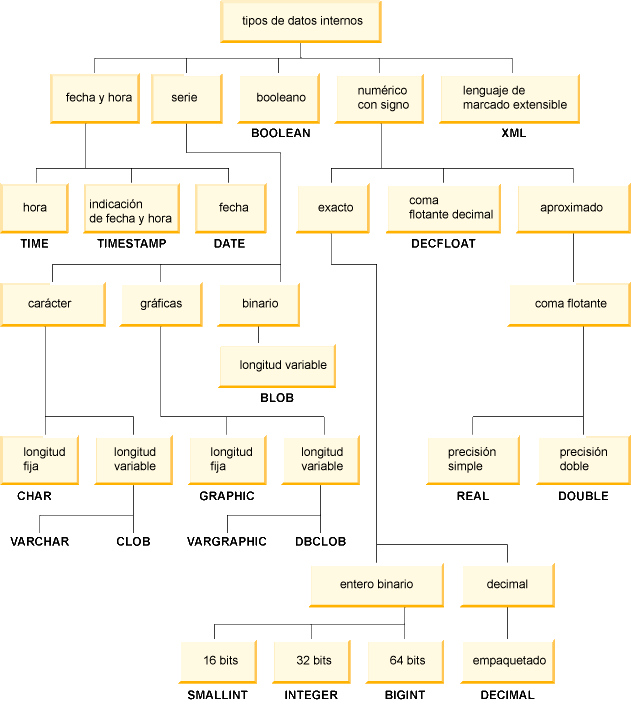
\includegraphics [scale=0.47]{capitulo2/images/tipos_datos_db2.png}
  \end{center}
 \caption{\label{Figura 23}Tipos de datos internos de DB2 soportados}
 \end{figure}
%%%%%%%%%%%%%%%%%%%%%%%%%%%%%%%%%%%%%%%%%%%%%%%%%%%%%%%%%%%%%%%%%%

\par \noindent \tn{Tipo de referencia}: Es un tipo compa�ero de un tipo estructurado. De
forma semejante a un tipo diferenciado, un tipo de referencia es un tipo escalar
que comparte una representaci�n com�n con uno de los tipos de datos internos. 
La representaci�n de este tipo se define cuando se crea el tipo
ra�z de una jerarqu�a de tipos.
Cuando un tipo de referencia es utilizado, se especifica un tipo estructurado
como par�metro del tipo. Este par�metro se denomina el tipo de destino de la
referencia. 

\par \noindent \tn{Tipo de matriz}: Un tipo de matriz definido por el usuario es un tipo
de datos que se define como matriz con elementos de otro tipo de datos. Cada tipo de matriz 
com�n tiene un �ndice con el tipo de datos INTEGER y tiene definida una cardinalidad m�xima. 
Cada matriz asociativa tiene un �ndice con el tipo de datos INTEGER o VARCHAR y
no tiene definida una cardinalidad m�xima. 

\par \noindent \tn{Tipo de fila}: Un tipo de fila es un tipo de datos que se describe
como una secuencia ordenada de campos con nombre, cada uno con un tipo de datos
asociado, que representa naturalmente una fila.
Un tipo de fila puede ser utilizada como tipo de datos para variables y
par�metros en SQL PL con el fin de suministrar una manipulaci�n sencilla de una
fila de datos.\\
\noindent Un tipo de fila incluye uno o m�s campos con tipos de datos asociados
que conforman una fila de datos. 

\par \noindent \tn{Tipo de cursor}: Es un tipo de datos definido por el usuario con la palabra clave CURSOR y opcionalmente con 
un tipo de fila asociado. Un tipo de cursor definido por el usuario con un tipo 
de fila asociado es un tipo de cursor de tipo firme (la tipificaci�n firme,
requiere tipos de datos coincidentes, lo que significa que es necesario convertir expl�citamente uno o ambos 
tipos de datos en un tipo de datos com�n antes de realizar comparaciones y asignaciones.); de lo contrario, es un tipo de cursor de tipo no firme. El valor de un tipo de cursor definido por el usuario 
representa una referencia a un cursor subyacente. 

\par \noindent Algunos ejemplos de utilizaci�n de definici�n de tipos de usuario
en DB2 son expuestos en el anexo \ref{anexo31} \\

\par \noindent \tn{Valores y
funciones XML}

\par \noindent DB2 proporciona los tipos de datos XML para almacenar documentos
XML bien formados. Un valor XML representa el XML con el formato que corresponde en
forma de documento XML, contenido XML o secuencia de nodos XML. Un valor XML que se encuentra almacenado en una tabla como valor de una columna definida con el
tipo de datos XML tiene que ser un documento XML con el formato correcto. Los
valores XML se procesan en una representaci�n interna que no puede ser comparada
con ning�n valor de serie. Un valor XML puede transformarse en un valor de cadena de caracteres serializada, 
representante del documento XML que utiliza la funci�n \ti{XMLSERIALIZE}. 
De igual manera, para almacenar datos XML en una columna de tipo de datos XML,
los datos deben ser transformados usando la funci�n \ti{XMLPARSE} \cite{ibm}.

\noindent A las expresiones que tienen como resultado un valor de tipo de
datos XML se les aplican restricciones especiales, estas expresiones y columnas
no se encuentran permitidas:

\begin{itemize}
  \item Una lista SELECT precedida por la cl�usula DISTINCT.
  \item Una cl�usula ORDER BY.
  \item Un predicado BETWEEN, IN o LIKE b�sico y cuantificado.
  \item Una cl�usula GROUP BY.
  \item Una subselecci�n de un operador de conjunto que no sea UNION ALL.
  \item Una funci�n agregada con DISTINCT.
\end{itemize}


\par \noindent \tn{Consultas SQL/XML}

\par \noindent Tal y como su nombre lo indica,
SQL/XML sirve como puente entre los mundos SQL y XML. Evolucion� como parte del est�ndar SQL
 que ahora incluye especificaciones para incrustar expresiones XQuery o XPath
  dentro de instrucciones SQL. XPath es un lenguaje que permite navegar por un documento XML 
  para realizar b�squedas de diferentes elementos y atributos. XQuery es
  compatible con XPath.
  Es relevante destacar que las expresiones XQuery (y XPath) distinguen
  may�sculas de min�sculas. Por ejemplo, una expresi�n XQuery que referencia al
  elemento XML ``rar'' no se aplicar� a los elementos XML denominados ``RAR'' o
  ``Rar''. 

\par \noindent DB2 suministra muchas otras funciones integradas para manipular
tipos de datos XML. A partir de la versi�n 9, DB2 admite una nueva Tecnolog�a
llamada XML pure, cuyas caracter�sticas son: 

\begin{itemize}
  \item XML es un tipo de dato.
  \item XML se indexa para apresurar b�squedas y recuperaci�n de datos.
  \item XML es gestionado y almacenado en un contenedor separado.
  \item XML se valida con esquemas en la base de datos.  
  \item Incorpora procedimientos para generar documentos XML en tablas.
  \item Incluye funciones para transformar XML en SQL y viceversa.
\end{itemize}

\par \noindent Las principales funciones XML con sus respectivos ejemplos son
especificadas en el anexo \ref{anexo32}.


\section{Oracle}

\noindent Una base de datos Oracle es una colecci�n de datos en uno o m�s
archivos. La base de datos contiene estructuras f�sicas y l�gicas. En el proceso
de crear una aplicaci�n, se crean estructuras como tablas e �ndices para
almacenar filas y acelerar su recuperaci�n. Se pueden crear sin�nimos por los
nombres de objetos, ver objetos en diferentes bases de datos (a trav�s de
enlaces a base de datos), y se puede restringir el acceso a los objetos. Incluso
se puede utilizar tablas externas para acceder archivos a fuera de la base de
datos como si las filas en los archivos fueran filas en tablas.

\noindent Debido a los requerimientos de las nuevas aplicaciones, desde su
versi�n 8, Oracle ha sido significativamente extendido con conceptos del modelo de bases de datos orientadas a objetos. 
De esta forma, aunque las estructuras de datos utilizadas para almacenar la
informaci�n siguen siendo tablas, los usuarios pueden utilizar muchos de los mecanismos de orientaci�n a objetos para definir y
acceder a los datos. Por este motivo, se dice que se trata de un modelo de datos
objeto relacional.

\noindent Este motor suministra mecanismos para que el usuario pueda definir
sus propios tipos de datos, cuya estructura puede ser compleja, y que pueden
ser aplicados para asignar un tipo a una columna de una tabla. Adem�s admite
el concepto de objetos, por lo que un objeto tiene un tipo, se almacena en
cierta fila de cierta tabla y posee un identificador �nico (OID). Dichos
identificadores pueden ser utilizados para referenciar a otros objetos y de
esta forma representar relaciones de asociaci�n y de agregaci�n. Tambi�n
se proporciona mecanismos para asociar m�todos a tipos, y constructores para
dise�ar tipos de datos multivaluados (colecciones) y tablas anidadas. 
La mayor deficiencia de este sistema es la imposibilidad de definir jerarqu�as 
de especializaci�n y herencia, lo cual es una importante desventaja con respecto
a las bases de datos orientadas a objetos. 

\par \noindent Ya que Oracle es el motor de base de datos escogido para la
implementaci�n y pruebas del presente estudio, como fue mencionado en los
objetivos del proyecto, se profundizar� en detalle sus
funciones, tipos de datos, objetos, entre otros.

\subsection{Tipos de datos colecci�n}

\par \noindent Para poder implementar relaciones 1:\ N, Oracle permite definir
el tipo colecci�n. Un dato de tipo colecci�n est� formado por un n�mero indefinido de elementos, todos del mismo tipo. De esta
manera, es posible almacenar en un atributo un conjunto de tuplas en forma de array (VARRAY), o en
forma de tabla anidada.
Los tipo colecci�n tambi�n tienen por defecto funciones
constructoras de colecciones cuyo nombre coincide con el del tipo. Los argumentos de entrada de
estas funciones son el conjunto de elementos que forman la colecci�n separados por comas y entre
par�ntesis, y el resultado es un valor del tipo colecci�n.
En Oracle es posible diferenciar entre un valor nulo y una colecci�n vac�a. Para construir una
colecci�n sin elementos se puede utilizar la funci�n constructora del tipo seguida por dos par�ntesis
sin elementos dentro.

\subsubsection{El tipo VARRAY}

\par \noindent Un array es un conjunto ordenado de elementos del mismo tipo. Cada elemento tiene asociado un
�ndice que indica su posici�n dentro del array. Oracle permite que los VARRAY sean de longitud
variable, aunque es necesario especificar un tama�o m�ximo cuando este es
declarado. Se puede utilizar el tipo VARRAY para:

\begin{itemize}
  \item Definir el tipo de dato de una columna de una tabla relacional.
  \item Definir el tipo de dato de un atributo de un tipo de objeto.
  \item Para definir una variable PL/SQL, un par�metro, o el tipo que devuelve
  una funci�n.
\end{itemize}

\par \noindent Cuando se declara un tipo VARRAY no se produce ninguna reserva de espacio. Si el espacio que
requiere lo permite, se almacena junto con el resto de columnas de su tabla, pero si es demasiado
largo (m�s de 4000 bytes) se almacena aparte de la tabla como un BLOB.
\noindent La principal limitaci�n del tipo VARRAY es que en las consultas es imposible poner condiciones
sobre los elementos almacenados dentro. Desde una consulta SQL, los valores de un VARRAY
solamente pueden ser accedidos y recuperados como un bloque. Es decir, no se puede acceder
individualmente a los elementos de un VARRAY. Sin embargo, desde un programa PL/SQL si que es
posible definir un bucle que itere sobre los elementos de un VARRAY.

\subsubsection{Tablas anidadas}

\par \noindent Una tabla anidada es un conjunto de elementos del mismo tipo sin ning�n orden predefinido. Estas
tablas solamente pueden tener una columna que puede ser de un tipo de datos b�sico de Oracle, o de
un tipo de objeto definido por el usuario. En este �ltimo caso, la tabla anidada tambi�n puede ser
considerada como una tabla con tantas columnas como atributos tenga el tipo de objeto.
\noindent Para relacionar las tuplas de una tabla
anidada con la tupla a la que pertenecen, se utiliza una columna oculta que aparece en la tabla
anidada por defecto. Todas las tuplas de una tabla anidada que pertenecen a la misma tupla tienen el
mismo valor en esta columna (\tn{NESTED\_TABLE\_ID}).
A diferencia de los \tn{VARRAY}, los elementos de las tablas anidadas
(\tn{NESTED\_TABLE}) s� pueden ser accedidos individualmente, y es posible poner
condiciones de recuperaci�n sobre ellos. En el anexo A.2.1 se muestra una forma
conveniente de acceder individualmente a los elementos de una tabla anidada mediante un cursor anidado. Adem�s, las tablas anidadas pueden estar indexadas. 

\noindent En la tabla \ref{tablavarray} se muestra una comparaci�n de
 ambos tipos de colecci�n.

\begin{table}[H]
\begin{center}
    \begin{tabular}{|l|l|l|} \hline
    ~                             & \tn{Varray}  & \tn{Nested table} \\ \hline
    Tama�o m�ximo                 & Si      & No           \\ \hline
    Borrado elementos individual  & No      & Si           \\ \hline
    Almacenamiento datos          & In-line & Out-of-line  \\ \hline
    Mantenimiento del orden       & Si      & No           \\ \hline
    \end{tabular}
    \caption{\label{tablavarray}Tipos colecci�n: Varray versus Nested Table}
    \end{center}
\end{table}

\subsection{Tipos de objetos}

\par \noindent El modelo relacional fue dise�ado para representar datos como una
serie de tablas con sus respectivas columnas y atributos. Oracle Database
11g es una base de datos objeto relacional, por lo que incorpora las tecnolog�as
orientadas al objeto. Gracias a esto, permite construir tipos de objetos
complejos, tales como:

\begin{itemize}
  \item Definir objetos dentro de objetos.
  \item Encapsular o asociar m�todos con dichos objetos.
\end{itemize}

\subsubsection{Estructura de un tipo de objeto}

\par \noindent Un tipo objeto se compone de dos partes: especificaci�n y cuerpo.
La especificaci�n organiza la interface a las aplicaciones; es donde se declaran
las estructuras de datos (grupo de atributos) y las operaciones (m�todos) que
son necesarios para la manipulaci�n de los datos. Por otro lado, el cuerpo es
lugar donde se definen los m�todos, por lo que es quien implementa la
especificaci�n. La estructura de un tipo de objeto es representa de forma
gr�fica en la figura \ref{Figura 24}.

\noindent En la especificaci�n se encuentra toda la informaci�n necesaria para
utilizar los m�todos. Es apropiado pensar que el cuerpo es como una caja negra y
la especificaci�n como la interface operacional. Y por esto mismo es posible
realizar cambios, optimizar o depurar el cuerpo sin la necesidad de modificar la
especificaci�n y con esto no afectar las aplicaciones cliente.

\noindent En la especificaci�n de tipo objeto los atributos se deben declarar
antes que cualquiera de los m�todos. Por lo que si la especificaci�n solamente
declara atributos, el cuerpo no es necesario. No es posible hacer declaraciones
de atributos en el cuerpo del tipo objeto.

%%%%%%%%%%%%%%%%%%%%%%%%%%%%%%%%%%%%%%%%%%%%%%%%%%%%%%%%%%%%%%%%%%%%%
 \begin{figure}[H]
 \begin{center}
  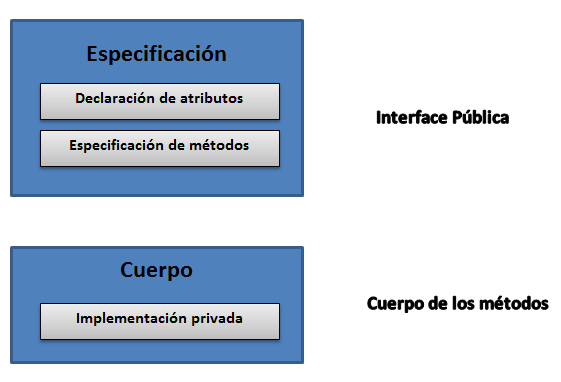
\includegraphics [scale=0.7]{capitulo2/images/estructura_tipo_objeto.png}
  \end{center}
 \caption[Estructura de un tipo de objeto]{\label{Figura 24}Estructura de un
 tipo de objeto \cite{ora2}}
 \end{figure}
%%%%%%%%%%%%%%%%%%%%%%%%%%%%%%%%%%%%%%%%%%%%%%%%%%%%%%%%%%%%%%%%%%

\noindent Todas las declaraciones en la especificaci�n del tipo son p�blicas,
por tanto, son visibles fuera del tipo objeto. No obstante, el cuerpo puede
tener declaraciones privadas, que definan m�todos necesarios para el
funcionamiento interno del objeto. El entorno de las declaraciones privadas es
local al cuerpo del objeto.
\noindent En el c�digo \ref{codigo40} se presenta un ejemplo para comprender
mejor esta estructura, en donde se define un tipo objeto para manipular n�meros complejos
con algunas operaciones, en el c�digo \ref{codigo41} se encuentra la creaci�n
del cuerpo del objeto y la definici�n de cada funci�n previamente declarada en
la especificaci�n.\\


\begin{lstlisting}[language=SQL, caption={Ejemplo creaci�n especificaci�n de
tipo objeto ORACLE}, label=codigo40] 
CREATE TYPE Complejo AS OBJECT (
	parte_real	REAL,	parte_imaginaria	REAL,
	MEMBER FUNCTION mas	(x Complejo) RETURN Complejo,
	MEMBER FUNCTION menos	(x Complejo) RETURN Complejo,
	MEMBER FUNCTION veces	(x Complejo) RETURN Complejo,
	MEMBER FUNCTION div_por	(x Complejo) RETURN Complejo);
\end{lstlisting}

%\newpage


\begin{lstlisting}[language=SQL, caption={Ejemplo creaci�n cuerpo de tipo objeto
ORACLE}, label=codigo41] 
CREATE TYPE BODY Complejo AS MEMBER FUNCTION mas(x Complejo) RETURN Complejo IS
	BEGIN
		RETURN Complejo(parte_real + x.parte_real, parte_imaginaria +
		x.parte_imaginaria);
	END mas;
	
	MEMBER FUNCTION menos (x Complejo) RETURN Complejo IS
	BEGIN
		RETURN Complejo(parte_real - x.parte_real, parte_imaginaria -
		x.parte_imaginaria);
	END menos;
	
	MEMBER FUNCTION veces (x Complejo) RETURN Complejo IS
	BEGIN
		RETURN Complejo(parte_real * x.parte_real - parte_imaginaria *
		x.parte_imaginaria, parte_real * x.parte_imaginaria + parte_imaginaria *
		x.parte_real);
	END veces;
	
	MEMBER FUNCTION div_por	(x Complejo) RETURN Complejo IS
	z REAL := x.parte_real**2 + x.parte_imaginaria**2;
	BEGIN
		RETURN Complejo((parte_real * x.parte_real + parte_imaginaria *
		x.parte_imaginaria) / z, (parte_imaginaria * x.parte_real - parte_real *
		x.parte_imaginaria) / z); 	END div_por;
\end{lstlisting}

\subsubsection{Componentes de un tipo objeto}

\par \noindent Un tipo objeto encapsula datos y operaciones, por este motivo en
la especificaci�n solamente se puede declarar atributos y m�todos, pero no
excepciones, constantes, tipos o cursores. Es requerido al menos un atributo,
pero los m�todos son opcionales.

\par \noindent As� como las variables, un atributo debe ser declarado mediante
un nombre y un tipo. El nombre tiene que ser �nico dentro del tipo objeto (pero
puede ser reutilizado en otros objetos) y el tipo puede ser cualquier tipo
excepto los siguientes:

\begin{itemize}
  \item LONG y LONG RAW.
  \item NCHAR, NCLOB y NVARCHAR2.
  \item MLSLABEL y ROWID.
  \item Los tipos espec�ficos de \tn{PL/SQL}: BINARY\_INTEGER (y todos sus
  subtipos), BOOLEAN, PLS\_INTEGER, RECORD, REF CURSOR, \ \%TYPE y \ \%ROWTYPE.
  \item Los tipos definidos en paquetes \tn{PL/SQL}.
\end{itemize}

\par \noindent No se puede inicializar un atributo en la declaraci�n utilizando
el operador de asignaci�n o cl�usula DEFAULT, de igual forma que no se permite
la restricci�n NOT NULL. Sin embargo, los objetos pueden ser almacenados en
tablas de la base de datos en que las que s� es posible imponer este tipo de
restricciones.
\noindent Se puede llegar a crear estructuras de datos muy complejas, por
ejemplo, el tipo de un atributo puede ser otro tipo de objeto (lo que ser�a un
tipo de objeto anidado).

\par \noindent Una definici�n simple para el concepto m�todo ser�a que es un
subprograma declarado en una especificaci�n de tipo mediante la palabra clave
\ti{MEMBER}. Un m�todo no puede tener el mismo nombre que el tipo de objeto ni
el de ninguno de sus atributos.
\noindent Muchos m�todos se componen de dos partes: especificaci�n y cuerpo. La
especificaci�n consta de nombre del m�todo, una lista opcional de par�metros y
en el caso de funciones de un tipo de retorno. El cuerpo es el c�digo que
ejecuta las operaciones especificadas. Para cada especificaci�n de m�todo de una
especificaci�n de tipo tiene que existir el correspondiente cuerpo del m�todo.



%\newpage
\subsubsection{Par�metro SELF}
\par \noindent Todos los m�todos de un tipo de objeto reciben como primer
par�metro una instancia predefinida del mismo tipo denominada
SELF. Indistintamente de que SELF sea declarado expl�cita o
impl�citamente, siempre es el primer par�metro pasado a un m�todo. 

\noindent El modo de acceso de SELF cuando no se declara expl�citamente es:

\begin{itemize}
  \item En procedimientos, si SELF no es declarado, su modo por omisi�n
es IN OUT.
\item En funciones miembro el acceso de SELF es IN.
\end{itemize}

\noindent En el cuerpo de un m�todo, SELF se�ala al objeto a partir del cual se
invoc� el m�todo. Los m�todos pueden hacer referencia a los atributos de SELF
sin necesidad de utilizar un cualificador.


\subsubsection{Sobrecarga}
\par \noindent Los m�todos del mismo tipo (funciones y procedimientos) pueden
ser sobrecargados, es  posible utilizar el mismo nombre para
m�todos distintos si sus par�metros formales difieren en n�mero, orden o tipo de
datos. Cuando uno de los m�todos es invocado, PL/SQL encuentra el cuerpo
adecuado comparando la lista de par�metros actuales con cada una de las listas
de par�metros formales. Sin embargo, la sobrecarga no es posible en el caso de
las siguientes situaciones:

\begin{itemize}
  \item Si los par�metros formales difieren s�lo en el modo.
  \item Si las funciones solamente difieren en el tipo de retorno.
\end{itemize}

\subsubsection{Constructores}
\par \noindent Cada tipo de objeto tiene un constructor que es una funci�n
definida por el sistema con el mismo nombre que el objeto. El constructor es
utilizado para inicializar y retornar una instancia de ese tipo de objeto.
Oracle genera un constructor por defecto para cada tipo de objeto. Los
par�metros del constructor coinciden con los atributos del tipo de objeto, es
decir, los par�metros y atributos son declarados en el mismo orden y poseen el
mismo nombre y tipo. Por otro lado, PL/SQL jam�s invoca al constructor
impl�citamente, por lo que el usuario debe llamarlo expl�citamente.




\subsection{Declaraci�n e inicializaci�n de objetos}
\par \noindent Una vez que un tipo de objeto ha sido definido y se ha instalado
en el esquema de la base de datos, este puede ser utilizado en cualquier bloque
PL/SQL.
Las instancias de los objetos son creadas en tiempo de ejecuci�n. En un bloque o subprograma, 
los objetos locales son instanciados
cuando se entra al bloque o subproprograma y estos dejan de existir cuando
sale del bloque o subprograma.
Por otro lado en un paquete, los objetos se instancian cuando se referencia por
primera vez al paquete y dejan de existir cuando finaliza la sesi�n. 
\noindent Los tipos de objetos se declaran del mismo modo que cualquier tipo interno. 

\par \noindent Adem�s es posible declarar objetos como par�metros formales de
funciones y procedimientos, por lo que es posible pasar objetos a los
subprogramas almacenados y de un subprograma a otro. 

\par \noindent Hasta que se inicializa un objeto, invocando al constructor para ese tipo de objeto, el objeto es
at�micamente nulo. Esto significa que el objeto es nulo, no s�lo sus atributos.
Un objeto nulo siempre es diferente a cualquier otro objeto. De hecho, la
comparaci�n de un objeto nulo con otro objeto siempre resulta NULL. Del mismo
modo, si se asigna un objeto con otro objeto at�micamente nulo, el primero se convierte a su vez en un 
objeto at�micamente nulo (y para poder utilizarlo debe ser reinicializado).
En resumen, si se asigna el no-valor NULL a un objeto, �ste se convierte en
at�micamente nulo, una buena
pr�ctica de programaci�n consiste en inicializar los objetos en su declaraci�n.

\par \noindent PL/SQL se comporta del siguiente modo cuando accede a objetos sin
inicializar:

\begin{itemize}
  \item La operaci�n de comparaci�n IS NULL siempre produce TRUE cuando se
  aplica a un objeto no inicializado o a cualquiera de sus atributos.
  \item Los atributos de un objeto no inicializado se eval�an en cualquier
  expresi�n como NULL.
  \item Intentar asignar valores a los atributos de un objeto sin inicializar
  provoca la excepci�n predefinida ACCESS\_INTO\_NULL.
\end{itemize}

\noindent La invocaci�n de los m�todos de un objeto no inicializado est�
permitida, pero en este caso:

\begin{itemize}
  \item SELF toma el valor NULL.
  \item Cuando los atributos de un objeto no inicializado son pasados como
  par�metros OUT o IN OUT, se produce una excepci�n si se intenta asignarles un
  valor.
\item Cuando los atributos de un objeto no inicializado se pasan como
par�metros IN, se eval�an como NULL.
\end{itemize}

\par \noindent Para poder acceder o cambiar los valores de un atributo se
utiliza la notaci�n punto ('.').  Los nombres de los atributos pueden encadenarse, lo que permite
acceder a los atributos de un tipo de objeto anidado. 

\subsection{Invocaci�n de constructores y m�todos}

\noindent La invocaci�n de un constructor est� permitida en cualquier punto en donde se puede invocar una funci�n.
Como las funciones, un constructor se invoca como parte de una expresi�n.

\par \noindent La especificaci�n de un m�todo se hace junto a la creaci�n de su
tipo y debe llevar siempre asociada una directiva de compilaci�n (PRAGMA
RESTRICT\_REFERENCES), para evitar que los m�todos manipulen la base de datos o
las variables del paquete PL/SQL. Se tienen las siguientes
directivas y su significado:

\begin{itemize}
\item WNDS: no se permite al m�todo modificar las tablas de la base de datos
\item WNPS: no se permite al m�todo modificar las variables del paquete PL/SQL
\item RNDS: no se permite al m�todo leer las tablas de la base de datos
\item RNPS: no se permite al m�todo leer las variables del paquete PL/SQL
\end{itemize}

\subsubsection{Paso de par�metros a un constructor}
\par \noindent Cuando los par�metros son enviados a un constructor la
invocaci�n asigna valores iniciales a los atributos del objeto que se est�
instanciando. Es necesario proveer par�metros para cada uno de los atributos ya
que, a diferencia de las constantes y variables, los atributos no poseen la
cl�usula DEFAULT.
Adem�s es posible invocar al constructor utilizando la notaci�n con nombre en
lugar de la notaci�n posicional.

\subsubsection{Invocaci�n de m�todos}
\par \noindent Como los subprogramas de un paquete,
los m�todos son invocados utilizando la notaci�n punto. 
\par \noindent Es posible encadenar los llamados a los m�todos, en donde la ejecuci�n se realiza de
izquierda a derecha.

\par \noindent En las sentencias SQL el llamado de un m�todos sin par�metros
requiere la lista vac�a de par�metros: '()'. En sentencias de procedimiento, 
la lista vac�ade par�metros es opcional, excepto cuando se encadenan
llamados, en dicho caso es obligatoria para todas las llamados excepto la �ltima.
No es posible encadenar llamados a m�todos adicionales a la derecha del
llamado de un procedimiento, puesto que los procedimientos no se invocan como
parte de una expresi�n. De la misma manera, cuando se encadenan dos llamados a una funci�n, el
resultado de la primera funci�n debe ser un objeto que puede ser pasado a la segunda funci�n.


\subsection{Compartici�n de objetos}

\par \noindent La mayor�a de los objetos del mundo real son considerablemente
m�s grandes y complejos que el tipo Relacional. Por ejemplo, considerar los
tipos de objeto del c�digo \ref{codigo59}, en donde los objetos tipo
\ti{Direcci�n} poseen m�s del doble de atributos que los del tipo
\ti{Relacional} y los objetos del tipo \ti{Persona} todav�a tiene m�s atributos,
incluyendo uno de tipo \ti{Direcci�n}.
Cuando objetos grandes son utilizados, resulta ineficiente enviar copias de �l
entre subprogramas. En dichas circunstancias es m�s adecuado compartir el
objeto. Esto es posible si el objeto cuenta con un identificador de objeto. \\

\begin{lstlisting}[language=SQL, caption={Ejemplo de objetos anidados en
ORACLE}, label=codigo59] 
CREATE TYPE Direccion AS OBJECT (
	direccion_calle VARCHAR2(35) , ciudad VARCHAR2(15) ,
	estado CHAR( 2 ) , cod_postal INTEGER) 
	/
CREATE TYPE Persona AS OBJECT (
	nombre VARCHAR2(15) , apellido VARCHAR2(15) ,
	fecha_nac DATE, direccion_casa Direccion, //Objeto anidado
	telefono VARCHAR2(15) , numero_seg_soc INTEGER) ;
\end{lstlisting}


\par \noindent Para compartir objetos se utilizan referencias. Una referencia es un puntero al objeto. 
\noindent La compartici�n de objetos proporciona dos ventajas importantes:

\begin{itemize}
  \item Cuando un objeto compartido es actualizado, el cambio se produce s�lo en
  un lugar y cualquier referencia al objeto puede recuperar los valores actualizados inmediatamente.
\item La informaci�n no se duplica innecesariamente.
\end{itemize}

\par \noindent En el c�digo \ref{codigo60} se visualizan las ventajas de 
compartir objetos, definiendo el tipo de objeto \ti{Hogar} y creando una tabla
que almacena las instancias de ese tipo. \\

\begin{lstlisting}[language=SQL, caption={Ejemplo tabla que almacena objetos en
ORACLE}, label=codigo60] 
CREATE TYPE Hogar AS OBJECT (
	direccion VARCHAR2(35), dueno VARCHAR2(25),
	estilo VARCHAR(15), precio REAL(9,2)) 	/
CREATE TABLE hogares OF Hogar;
\end{lstlisting}


\subsubsection{Utilizaci�n de referencias}

\par \noindent Con el objeto de tipo \ti{Persona} del ejemplo del c�digo
\ref{codigo59}, se puede dise�ar una comunidad que pueda compartir
la misma casa (Hogar). Para ello se puede utilizar el modificador de tipo REF,
ver c�digo \ref{codigo61}, el cual declara una referencia (almacena un
puntero al objeto). Es relevante destacar c�mo las referencias entre personas y
Hogares y entre personas entre s� definen relaciones que existen en el mundo
real. \\


\begin{lstlisting}[language=SQL, caption={Ejemplo de modificador REF en objetos
en ORACLE}, label=codigo61] 
CREATE TYPE Persona AS OBJECT (
	nombre VARCHAR2(15) ,
	apellido VARCHAR2(15) ,
	fecha_nac DATE,
	direccion_casa REF Home, //Compartido con la familia
	telefono VARCHAR2(15) ,
	numero_seg_soc INTEGER
	madre REF Persona , // Miembros de la familia
	padre REF Persona ,
	...) ;
/
\end{lstlisting}

\par \noindent 
Es posible declarar referencias como variables, par�metros, campos o atributos.
Tambi�n, se pueden utilizar referencias como par�metros IN y OUT en funciones y
procedimientos. Sin embargo, no es posible navegar a trav�s de referencias. En
el ejemplo del c�digo \ref{codigo62} se muestra un intento ilegal de navegar a
trav�s de una referencia a un objeto. Para poder realizar esta
operaci�n es preciso utilizar el operador DEREF, a trav�s del cual se puede
acceder al objeto. \\

\begin{lstlisting}[language=SQL, caption={Ejemplo de utilizaci�n err�nea de REF
en objetos ORACLE}, label=codigo62] 
DECLARE
	persona_ref REF Persona;
	num_telefono VARCHAR2(15) ;
BEGIN
	...
	num_telefono = persona_ref.telefono; // es Ilegal!
\end{lstlisting}


\subsubsection{Limitaciones en la definici�n de tipos}

\par \noindent En la creaci�n de un tipo solamente es posible hacer referencia a
objetos que existen en el esquema de objetos. Para poder solucionar este problema se emplea una sentencia \ti{CREATE TYPE}
especial denominada \ti{definici�n previa} de tipo, la cual permite la creaci�n
de tipos de objetos mutuamente dependientes. Para resolver el problema
mencionado previamente, basta con crear el objeto antes de hacer la referencia.
El tipo creado a trav�s de una definici�n previa de tipo tiene como nombre \ti{tipo de objeto incompleto}, ya que carece
de atributos y m�todos hasta que se defina por completo.

\par \noindent Un tipo incompleto impuro posee atributos, pero compila con
errores sem�nticos (no sint�cticos) al hacer referencia a un tipo indefinido.


\subsection{Manipulaci�n de objetos}
\par \noindent Es posible utilizar un tipo de objeto en la sentencia \ti{CREATE
TABLE} para especificar el tipo de una columna. Cuando la tabla se ha
creado, se pueden utilizar las sentencias SQL para insertar un objeto,
seleccionar sus atributos, invocar los m�todos definidos y actualizar su estado.
Ese preciso utilizar un alias de la tabla cuando se hace referencia a un atributo o m�todo. Cuando se
crea un objeto de esta forma, este carece de identidad fuera de la tabla de la
base de datos. Sin embargo, el tipo de objeto existe independientemente de
cualquier tabla y puede ser utilizado para crear objetos mediante otros
m�todos.



\par \noindent En el c�digo \ref{codigo67} se puede observar como se crea una
tabla que almacena en sus filas objetos del tipo \ti{Relacional}. Este tipo de tablas, en
las que sus filas contienen un tipo de objetos, son llamadas tablas de objetos, donde cada columna en una fila corresponde con un atributo del tipo de
objeto. Cada fila en una tabla de objetos cuenta con un identificador de objeto,
que identifica de forma �nica al objeto almacenado en esa fila y sirve como una
referencia al objeto. \\


\begin{lstlisting}[language=SQL, caption={Ejemplo creaci�n de tabla de objetos
ORACLE}, label=codigo67] 
CREATE TABLE numeros_relacionales OF Racional ;
\end{lstlisting}


\subsubsection{Selecci�n de objetos}

\par \noindent En el c�digo \ref{codigo68} se crea un tipo de objeto denominado
\ti{Persona} y una tabla de objetos Personas junto con algunos valores. Por otro
lado la subconsulta del c�digo \ref{codigo69} produce como resultado un conjunto
de filas que tienen solamente atributos de los objetos \ti{Persona}. \\



\begin{lstlisting}[language=SQL, caption={Ejemplo tabla de objetos ORACLE},
label=codigo68] 
CREATE TYPE Persona AS OBJECT (
	nombre VARCHAR2(15), apellido VARCHAR2(15),
	fecha_nac DATE, direccion_casa Direccion, telefono VARCHAR2(15)) ; /
	
CREATE TABLE Personas OF Persona; /
\end{lstlisting}

\begin{lstlisting}[language=SQL, caption={Ejemplo de selecci�n de objetos
ORACLE}, label=codigo69] BEGIN
	INSERT INTO Empleados //Otra tabla de objetos de tipo Persona
	SELECT * FROM Personas per WHERE per.apellido LIKE '% Tarantino';
\end{lstlisting}


\subsubsection{El operador VALUE}
\par \noindent Como su nombre lo dice, este operador devuelve el valor de un
objeto. VALUE requiere como argumento una variable de correlaci�n (para este
contexto, ser�a una fila o alias de tabla asociado a una fila en una tabla de
objetos). Para obtener un conjunto de objetos se puede
utilizar el comando VALUES. Las reglas de integridad, de clave primaria, y el resto de propiedades que se definan sobre una tabla, 
s�lo afectan a los objetos de esa tabla, es decir no se refieren a todos los objetos del tipo asignado a 
la tabla. 


\subsubsection{El operador REF}
\par \noindent Los identificadores �nicos asignados por Oracle a los objetos que se almacenan en una tabla, 
permiten que �stos puedan ser referenciados desde los atributos de otros objetos o desde las 
columnas de tablas. El tipo de datos proporcionado por Oracle para soportar esta facilidad se 
denomina REF. Un atributo de tipo REF almacena una referencia a un objeto del tipo definido, e 
implementa una relaci�n de asociaci�n entre los dos tipos de objetos. Estas referencias se pueden 
utilizar para acceder a los objetos referenciados y para modificarlos; sin embargo, no es posible 
operar sobre ellas directamente. Para asignar o actualizar una referencia se debe utilizar siempre REF
o NULL. 

\noindent Cuando se define una columna de un tipo a REF, es posible restringir su dominio a los objetos que se 
almacenen en cierta tabla. Si la referencia no se asocia a una tabla sino que s�lo se restringe a un tipo 
de objeto, se podr� actualizar a una referencia a un objeto del tipo adecuado con independencia de la 
tabla donde se almacene. En este caso su almacenamiento requerir� m�s espacio y su acceso ser� 
menos eficiente. 


\subsubsection{Referencias colgadas (\ti{dangling refs})}

\par \noindent
Cuando se borran objetos de la base de datos, puede ocurrir que
otros objetos que referencien a los borrados queden en estado inconsistente. 
Estas referencias se denominan dangling references, y Oracle 
proporciona el predicado llamado IS DANGLING que permite comprobar cu�ndo sucede esto.


\subsubsection{El operador DEREF}
\par \noindent No es posible navegar a trav�s de referencias en procedimientos
SQL. Debido a esto se hace necesario emplear el operador DEREF (derreferenciar
un puntero es obtener el valor al cual este apunta). Este operador tiene
como argumento una referencia a un objeto y retorna el valor de dicho objeto. Si
la referencia est� pendiente, DEREF devuelve el valor NULL.
En esta situaci�n no es obligatorio especificar una tabla de objetos ni un criterio de
b�squeda, ya que cada objeto almacenado en una tabla de objetos cuenta con un
identificador de objeto �nico y est�tico que es parte de cada referencia a un
objeto. 

\par \noindent Adem�s es posible la utilizaci�n del operador DEREF en sentencias
SQL sucesivas para derreferencias referencias.

\par \noindent En procedimientos SQL la utilizaci�n del operador DEREF es ilegal. En sentencias SQL se puede utilizar
la notaci�n punto para navegar a trav�s de referencias. 


\subsubsection{Inserci�n de objetos}
\par \noindent Para almacenar objetos en una tabla de objetos se utiliza el
comando UPDATE.  Por otro lado, adem�s es posible utilizar la cl�usula RETURNING,
la cual almacena una referencia a un objeto en una variable local. Es
necesario recalcar como esta cl�usula simula una sentencia SELECT. La cla�sula
RETURNING puede ser utilizada tambi�n en sentencias UPDATE y DELETE. Para
ingresar objetos en una tabla de objetos se puede emplear una consulta que retorne un objeto del
mismo tipo.


\subsubsection{Actualizaci�n de objetos}
\par \noindent Para poder modificar los atributos de un objeto en una tabla de
objetos se debe utilizar la sentencia UPDATE.


\subsubsection{Eliminaci�n de objetos}

\par \noindent Para la eliminaci�n de objetos (filas) en una tabla de objetos se
utiliza la sentencia SQL DELETE. Para eliminar objetos selectivamente se utiliza la
cl�usula WHERE.

\subsection{Herencia}

\par \noindent Desde la versi�n 9i de Oracle se incorpora la herencia simple de
tipos, sin embargo a�n no se soporta la herencia de tablas, lo cual si posee
soporte en el standard SQL 2003. El tipo ra�z de una jerarqu�a se crea empleando 
la sentencia CREATE TYPE y debe ser declarado como NOT FINAL. La opci�n por 
defecto es FINAL (indicando as�, que pueden derivarse subtipos de �l). En la
figura \ref{herencia1} se muestra un ejemplo t�pico de una persona que se
especiliza en estudiante y empleado, su implementaci�n se encuentra detallada en
el c�digo \ref{codher1}.


 \begin{figure}[H]
 \begin{center}
  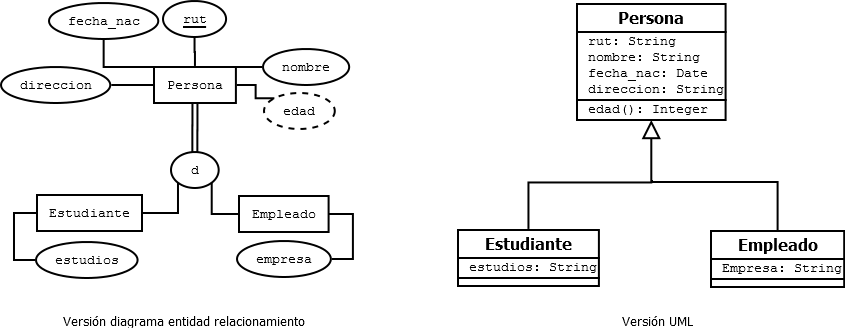
\includegraphics [scale=0.5]{capitulo2/images/herencia.png} \end{center}
 \caption{\label{herencia1}Ejemplo de herencia}
 \end{figure}

\begin{lstlisting}[language=SQL, caption={Ejemplo de implementaci�n de herencia
de objetos en ORACLE}, label=codher1] 
CREATE TYPE tPersona AS OBJECT (
	rut		VARCHAR(9),
	nombre	VARCHAR(25),
	fecha_nac	DATE,
	direccion	VARCHAR(1000),
	MEMBER FUNCTION edad RETURN NUMBER)
	NOT INSTANTIABLE NOT FINAL 	/
CREATE TYPE tEstudiante UNDER tPersona (estudios VARCHAR(50));/
CREATE TYPE tEmpleado UNDER tPersona (empresa VARCHAR(50)); /
\end{lstlisting}

\par \noindent La herencia simple de tipos que contempla Oracle implica que
cualquier subtipo herede de su padre los m�todos y atributos que este posea.
Es as� como para el ejemplo presentado en el c�digo \ref{codher1}, los subtipos
tEstudiante y tEmpleado poseen la funci�n edad(). Por lo tanto, esta funci�n
podr� ser llamada sobre cualquier instancia de estos tipos, es decir, 
cuando se defina una tabla de cualquiera de los 
dos subtipos, se podr� invocar a la funci�n 
edad() sobre cualquiera de las filas de la tabla. 

\par \noindent Es sumamente importante tener en cuenta que Oracle
no soporta la herencia de tablas; es decir, la definici�n de jerarqu�as de tablas sobre tipos 
que est�n integrados en una jerarqu�a de tipos. Oracle s�lo permite asegurar que los atributos y 
m�todos del supertipo de la tabla padre se heredar�n en las tablas definidas sobre los 
subtipos. Sin embargo, las restricciones, disparadores, etc. definidos para una tabla no podr�n ser 
heredados por otras tablas, aunque sus tipos subyacentes pertenezcan a la misma
jerarqu�a. En el c�digo \ref{codher2} se muestran las sentencias para 
crear las tablas del tipo padre y de los dos 
subtipos, como se observa es necesario definir en cada tabla sus propias 
restricciones, ya que �stas no se propagan.\\

\begin{lstlisting}[language=SQL, caption={Ejemplo de creaci�n de tabla del tipo
padre y de subtipos ORACLE}, label=codher2] 
CREATE TABLE Persona OF tPersona
	(PRIMARY KEY (rut),
	 CHECK(direccion like (�%Tocopilla%�)));
	 
CREATE TABLE Estudiante OF tEstudiante
	(PRIMARY KEY (nombre));
	
CREATE TABLE Empleado OF tEmpleado
	(PRIMARY KEY (rut));
\end{lstlisting}

\par \noindent Las tablas Estudiante y Empleado definidas sobre 
subtipos del tipo tPersona no deben cumplir en 
absoluto las restricciones impuestas para la tabla 
Persona definida sobre el tipo padre tPersona. As�, por ejemplo, se puede
insertar en la tabla Empleado una fila en la que el valor del atributo
direcci�n no contenga la cadena ``Tocopilla'', mientras que en la tabla 
Persona eso ser�a imposible. Del mismo modo, se puede definir el campo nombre
como clave primaria en la tabla Estudiante, aunque en la tabla 
padre Persona la clave primaria se defini� sobre el 
campo rut.

\noindent Pero, adem�s de que las tablas no hereden las 
restricciones de la tabla definida para el supertipo, existe 
un problema aun mayor y este se presenta en el ejemplo del c�digo \ref{codher2},
ya que no se puede rescatar el hecho impl�cito que existe en toda jerarqu�a, de
que todo estudiante es persona y de que todo empleado es persona. Esto se debe a que no existe relaci�n alguna entre las 
tablas, no hay nada que le indique al SABD que un 
empleado o un alumno es adem�s una persona. Por 
ello, al realizar una consulta a persona, se obtendr�a 
s�lo aquellas personas que no fueran ni estudiantes ni 
empleados.

\noindent De esta forma, para la implementaci�n de 
una jerarqu�a en Oracle, aunque es posible apoyarse en ocasiones en la
utilizaci�n de la herencia de tipos, se necesita 
adem�s recurrir a los cl�sicos 
mecanismos empleados en las bases de datos relacionales (claves for�neas, o
referencias, entre las tablas, restricciones, vistas, entre otros.).



\subsection{Valores y funciones XML}

\par \noindent La base de datos XML de Oracle, referencia a una colecci�n de
tecnolog�as XML nativas en el servidor de base de datos. Sin embargo, el soporte nativo XML 
es s�lo una parte de la infraestructura XML en Oracle. La infraestructura XML general proporciona soporte XML nativo 
de alto rendimiento y una plataforma extensible en el que los usuarios pueden crear y desplegar sus propias soluciones.
En el motor nativo XML, las tablas y vistas XMLType ofrecen el
almacenamiento de datos XML. El repositorio de base de datos XML proporciona un
repositorio de documentos XML que se ha optimizado para el manejo de documentos
XML. PL/SQL y las funciones SQL/XML permiten operaciones de XML en datos SQL 
y contenido XML. 

\subsubsection{Tipo de dato XML}

\par \noindent Este mapeado de la estructura XML a la estructura de la base de datos en Oracle se 
realiza con el tipo XMLType, que es un tipo abstracto. El tipo XMLType se almacena en un 
tipo CLOB, aunque puede asociarse a un esquema XML para la definici�n de su
estructura lo que obliga que cualquier documento sea validado con este esquema. En este segundo caso el 
esquema del documento se modela en la estructura objeto relacional de la base de
datos.
La ventaja de hacerlo de la primera manera es que todo tipo de documentos XML 
pueden almacenarse en ese elemento XMLType. La segunda obliga a que el elemento sea 
v�lido frente al esquema asociado, aunque su mapeado en la estructura objeto
relacional permite tratar el documento de manera m�s eficiente y flexible.

\subsubsection{Mapeado de XMLType dado un esquema XML}

\par \noindent Los elementos del esquema XML son mapeados como objetos en los
que cada elemento anidado de tipo simple es representado por un atributo de un tipo nativo lo m�s acorde 
posible con el tipo del esquema por ejemplo si es un n�mero con NUMBER, si es
texto con VARCHAR, etc. Aun as� es posible forzar la representaci�n del elemento
a un tipo de Oracle mediante el atributo SQLType utilizado en el elemento del esquema.
\noindent Cuando un elemento contiene un elemento complejo, este es modelado con un objeto 
y el elemento padre establece una referencia a �l con tipos referencia. Es posible forzar que 
el mapeado de los tipos complejos se realice en CLOB, NCLOB o VARCHAR (sin ser
representados en el modelo objeto relacional) mediante el atributo SQLType
(=CLOB) utilizado en el elemento del esquema.
\noindent Cuando la ocurrencia de un elemento, ya sea simple o complejo, es
mayor que uno el elemento es representado en el objeto padre con un array variable si el n�mero de 
ocurrencias m�ximas es finito o con un tabla anidada si es infinito.

\subsubsection{Crear tables y/o columnas XMLType}

\par \noindent Para crear columnas o tablas XMLType se hace de la misma
forma que al definir columnas o tablas de objetos. Para definir una columna o tabla XMLType 
asociada a un esquema se debe registrar 
primero el esquema en la base de datos. Esto se realiza mediante la librer�a 
DBMS\_XMLSCHEMA que posee dos funciones: registerSchema para registrar el
esquema y deleteSchema para eliminar el registro. Una vez registrado el esquema
se puede crear columnas y tablas XMLType asociadas empleando el comando
XMLSCHEMA.

\subsubsection{Insertar documentos XML}

\par \noindent Si se tratan a los tipos XMLType como objetos se puede utilizar
el constructor de dichos objetos para instanciar nuevos elementos XMLType, tomando como par�metro la 
cadena que representa al documento XML. En el c�digo \ref{xmlora1} se presenta
un ejemplo de utilizaci�n. \\

\begin{lstlisting}[language=SQL, caption={Ejemplo de inserci�n de
datos utilizando XMLTYPE en ORACLE}, label=xmlora1] 
INSERT INTO warehouses VALUES
	( 100, XMLType(
		'<Warehouse whNo="100">
		<Building>Owned</Building>
		</Warehouse>'),	'Tower Records', 1003);
	
UPDATE warehouses SET warehouse_spec = XMLType
	('<Warehouse whono="200">
	<Building>Leased</Building>
	</Warehouse>');
\end{lstlisting}

\subsubsection{Consultar documentos XML}

\par \noindent Es posible rescatar un documento en forma de CLOB, VARCHAR o
NUMBER mediante los m�todos de XMLType: getClobVal, getStringVal, getNumberVal. Con estas funciones 
simplemente se obtiene el documento XML convertido en un tipo nativo. 
Las consultas no s�lo son de recuperaci�n de documentos completos, es posible
adem�s recuperar partes del documento y efectuar predicados de selecci�n en
partes del documento.
Estas partes est�n basadas en la estructura DOM de XML y se se�alan haciendo uso
de XPath.
Las funciones incluidas con este prop�sito son extract y existsNode: el primero devuelve el nodo 
del documento XML (de la estructura DOM) solicitado y el segundo devuelve verdadero (1) 
cuando existe el nodo solicitado. 

\par \noindent El comando extract siempre devuelve el nodo en un tipo XMLType,
si se desea recuperar el valor del nodo de texto de ese nodo se puede utilizar
getNumberVal o getStringVal sobre el elemento XMLType retornado. Tambi�n se
puede utilizar extractValue que tiene una sintaxis id�ntica a extract pero que devuelve el valor del nodo de texto y no el 
elemento XMLType. Estas funciones s�lo son v�lidas para nodos que tengan un solo y �nico 
nodo de texto. El comando updateXML permite actualizar el valor de algunos nodos se�alados del 
documento XML, para evitar de esa manera modificar todo el documento cuando s�lo var�a 
parte de el. Sus par�metros son parejas de rutas XPath y valores, donde la ruta
se�ala el nodo a modificar y los valores sustituir�n a los antiguos de ese nodo.

\par \noindent El comando XMLTransform toma como par�metros dos instancias de XMLtype siendo la 
primera el documento de origen y la segunda un documento XSLT de
transformaciones XML y devuelve el documento resultante de la transformaci�n XML. Un sin�nimo de este comando 
es el m�todo XMLTransform de la clase XMLType.  
\noindent Es posible validar documentos XML frente a esquemas XML mediante el comando 
XMLisValid y el m�todo de XMLType isSchemaValidated. Ambos devuelven verdadero (1) si el 
documento se valida correctamente. 

\subsubsection{SQLX}

\par \noindent Al igual que en el modelado objeto relacional, en el que no es
necesario convertir los datos en el modelo plano relacional al modelo objeto
relacional para trabajar con ellos en este �ltimo modelo, es posible
mediante comandos y vistas representar datos del modelo relacional u objeto
relacional como documentos XML sin la necesidad de modificarlos.

\noindent Oracle soporta cinco comandos del est�ndar SQLX (SQL to XML, SQL/XML)
para la representaci�n de datos relacionales con XML: XMLElement, XMLForest, XMLConcat, 
XMLAttributes y XMLAgg. Tambi�n soporta XMLColAttVal como comando SQLX propio, pero 
a�n no aceptado en el est�ndar. Estos comandos permiten representar datos como un 
documento XML cuya estructura de ese documento es definida por los
desarrolladores.

\noindent Oracle, tambi�n, soporta las funciones SYS\_XMLGEN, SYS\_XMLAGG, 
XMLSEQUENCE y XMLFormat con el mismo prop�sito que las anteriores pero sin ser parte del est�ndar SQLX o 
de su propuesta. 
Es posible adem�s crear vistas del tipo XMLType para representar tablas y vistas 
relacionales como documentos XML de forma transparente para la consulta, como si de una 
consulta a un XMLType se tratase.

\par \noindent XMLElement es una funci�n que devuelve un tipo XMLType dados como par�metros el 
nombre del elemento XML, una serie de atributos y el contenido del nodo. El XMLType 
retornado es un nodo con el nombre del primer par�metro, los atributos del
segundo y el contenido de los �ltimos par�metros. El contenido puede ser un valor o un nuevo elemento 
XMLType para poder formar la estructura anidada de los documentos XML.

\noindent Los atributos se definen mediante la funci�n XMLAttributes que toman como m�todo el 
listado de atributos a asignar al elemento XML. Si no se especifica la cl�usula AS en cada 
atributo se deja como nombre de atributo el inferido de la estructura
relacional, si se utiliza AS se deja el indicado.

\noindent La funci�n XMLForest crea un �rbol XML de los par�metros que toma. Un �rbol XML 
son nodos situados a la misma altura, esto significa nodos que partir�an del
mismo nodo ra�z, salvo que no se haya definido este nodo ra�z. Cuando el
par�metro es acompa�ado de la cl�usula AS, se �ste es utilizado como nombre de
elemento XML, cuando no se infiere de la estructura de los datos.

\noindent La funci�n XMLConcat, concatena los par�metros dados uno tras otro en el orden en que aparecen como 
par�metros, estos pueden
ser una secuencia de elementos XMLTYPE o datos tipo XMLType. Mientras que en
XMLForest los par�metros son datos relacionales, en XMLConcat son tipos XMLType.

\noindent La funci�n XMLAgg es una funci�n de agregado que produce un bosque de elementos 
XML dada una colecci�n de elementos. Se usa normalmente con consultas con cl�usulas de 
agrupaci�n como GROUP BY.

\noindent La funci�n XMLColAttVal crea un �rbol de XML donde cada elemento es de tipo column
y posee un atributo tipo name con el nombre del elemento, especificado por AS en los 
par�metros o inferido de los datos.

\noindent La funci�n SYS\_XMLAGG engloba todos los documentos XML o fragmentos
de una expresi�n en un solo documento XML. La etiqueta que engloba es por defecto ROWSET, pero 
puede ser definida con XMLFormat. 

\noindent XMLSEQUENCE devuelve una secuencia (array variable) de XMLType dado un 
XMLType. En consecuencia, toma los nodos hijo directos del XMLType y devuelve un
nodo XMLType por cada uno de ellos en un objeto XMLSequenceType. 

\noindent La funci�n SYS\_XMLGEN toma un tipo nativo, un tipo abstracto o un
tipo XMLType y genera con �l un documento XML. Si es un tipo nativo forma una etiqueta con el valor 
dentro, si es un tipo abstracto mapea los atributos del tipo abstracto a un documento XML y 
si es un XMLType engloba a este elemento en otro elemento de nombre por defecto ROW. Es 
posible indicar el nombre de la etiqueta principal del documento XML generado mediante la 
funci�n XMLFormat.

\noindent El objeto XMLFormat es un par�metro de SYS\_XMLGEN y SYS\_XMLAGG. Este
objeto define las caracter�sticas del documento generado por estas dos funciones mediante sus 
atributos. Si se desea cambiar el formato del documento XML generado tan solo
se tendr� que dar el valor adecuado al correspondiente atributo de XMLFormat.

\subsubsection{Vistas XMLType}

\noindent Las vistas XMLType permiten tomar elementos relacionales u objeto
relacionales de la base de datos, sin modificar ni los datos ni su estructura
para poder mostrarlos como si fuesen documentos XML.
Mediante la creaci�n de vistas habitual se crea una vista indicando que es de
tipo XMLType (OF XMLTYPE), la cl�usula OBJECT ID indica que columna ser� el
identificador �nico de cada elemento y que el tipo XMLType se almacenar� en la columna
sys\_nc\_rowinfo\$.

\noindent Adem�s es posible crear vistas XMLType mapeando los datos relacionales
mediante un esquema y no con el comando SELECT de la definici�n de la vista. El esquema define el 
mapeado de cada elemento a la columna de datos mediante el atributo xdb:SQLName en el 
elemento del esquema, de tal manera que el elemento contendr� el valor de la columna 
indicada en ese atributo.

\par \noindent En el anexo \ref{anexo42} se presentan ejemplos de cada secci�n
vista de XML.

\subsubsection{Dise�ando la base de datos XML}

\par \noindent Cuando se comienza a dise�ar aplicaciones con Oracle XML DB, se
necesita tomar varias decisiones, incluyendo como almacenar los datos XML en la
base de datos, cu�l es la estrategia para recuperar o generar los datos XML, y
c�mo crear �ndices apropiados para buscar el contenido en documentos XML. \\
%\newpage
\par \noindent \tn{C�mo almacenar datos XML}

\par \noindent Existen tres caminos diferentes para almacenar documentos dentro
Oracle, y cada uno de ellos ofrece compensaciones en rendimiento y
funcionalidad. En la figura \ref{flow} se presenta un diagrama de flujo que
sirve de ayuda para simplificar la selecci�n. En el anexo \ref{anexo421} se
detalla en profundidad los pasos mencionados en dicho diagrama.

%%%%%%%%%%%%%%%%%%%%%%%%%%%%%%%%%%%%%%%%%%%%%%%%%%%%%%%%%%%%%%%%%%%%%
 \begin{figure}[!hbtp]
 \begin{center}
  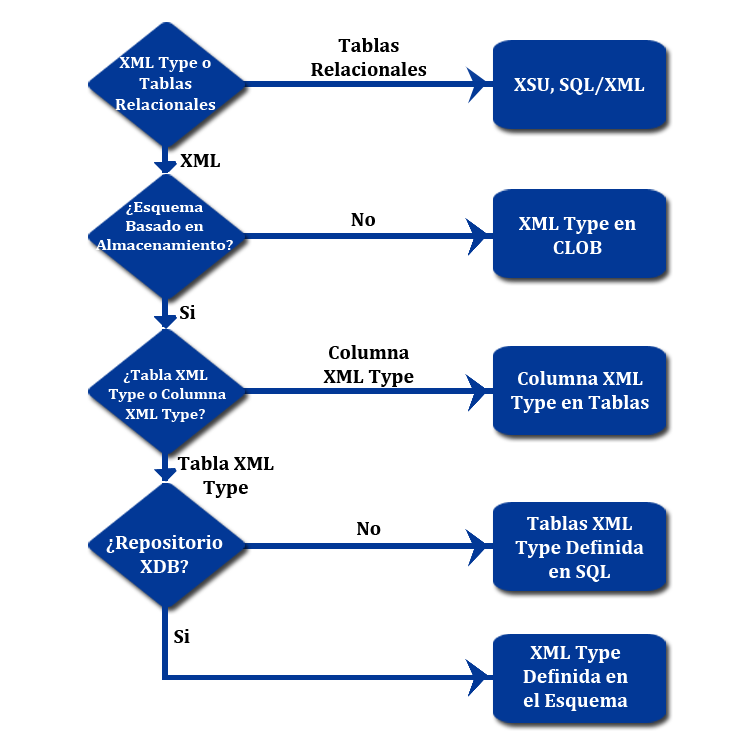
\includegraphics [scale=0.485]{capitulo2/images/diagrama_deciciones_xml.png}
  \end{center} \caption[Diagrama de flujo de decisi�n para almacenar XML en
 Oracle]{\label{flow}Diagrama de flujo de decisi�n para
  almacenar XML en Oracle \cite{wang}}
 \end{figure}
%%%%%%%%%%%%%%%%%%%%%%%%%%%%%%%%%%%%%%%%%%%%%%%%%%%%%%%%%%%%%%%%%%

% \newpage
% \section{Mapeo objeto relacional (ORM)}



%\subsubsection{Hibernate}



 \chapter{CASO DE ESTUDIO} \label{cap3}

\noindent En este cap�tulo se presenta un caso de estudio que permite
implementar la teor�a en los diferentes modelos. As� mismo,  gracias a este caso de estudio se
pretende demostrar la importancia de la utilizaci�n del modelo objeto relacional
y XML, ya que, mientras el modelo relacional es muy sencillo de implementar por
ser el m�s utilizado, el objeto relacional posee una mayor sem�ntica que se hace
muy familiar si se tiene conocimientos del paradigma orientaci�n al objeto. 

\section{Descripci�n del Caso de Estudio} \label{enunciado}
\noindent Este caso de estudio, es un caso real al cual la memorista se vi�
enfrentada, no obstante su implementaci�n fue llevada a cabo en una base de datos relacional
pura.

\noindent Se debe desarrollar e integrar un nuevo m�dulo para
un sistema de gesti�n escolar, dicho m�dulo consiste en implementar las planificaciones curriculares de los 
profesores seg�n curso y asignatura, a modo de automatizar el proceso actual que se realiza 
en planillas en papel. 

\noindent Un nivel de ense�anza es el nivel al que pertenece un curso, por
ejemplo 1� B�sico, 2� B�sico, etc. Un nivel de ense�anza posee un identificador y un nombre.
Como es sabido un curso (8�A) tiene un profesor jefe, a�o (el 8�A del 2013), asignaturas y 
alumnos. Por ejemplo, el 8�A tiene como profesor jefe a ``Nelson N��ez'', cabe
mencionar que todos los octavos tienen las mismas asignaturas. En el m�dulo s�lo es necesario tener 
conocimiento sobre profesores y asignaturas.

\noindent Una asignatura posee un id y nombre. Considere que cada asignatura
tiene un id distinto para cada nivel por ejemplo: Lenguaje y Comunicaci�n del nivel de ense�anza 7� B�sico tiene un 
c�digo distinto que para los 8� B�sicos. Una asignatura es dictada en todos los cursos del 
mismo nivel de ense�anza (8�A, 8�B, 8�C, etc.), adem�s por cada curso asignatura existe un 
profesor. Por ejemplo, en el 8�A la asignatura ``Matem�ticas'' es dictada por
John P�rez y Educaci�n F�sica por Robert Rodr�guez y matem�ticas para el 8�B es dictada por Juan Soto.
Del profesor interesa el rut, nombres, apellido paterno, apellido materno, fecha de nacimiento, 
cantidad de cursos en los que hace clase.

\noindent Por otro lado existe el concepto de ``tipo de programa'' el cual tiene
su identificador, nombre, y abreviatura. Existen 5 tipos de programas base:

\begin{itemize}
  \item Unidades educativas.
  \item Objetivos fundamentales verticales.
  \item Objetivos fundamentales transversales.
  \item Aprendizajes esperados.
  \item Contenidos m�nimos obligatorios.  
\end{itemize}

\noindent Un tipo de programa posee muchos detalles de programa
(curricular), el cual tiene un identificador, descripci�n, nombre y asignatura asociada. Por ejemplo, para los 8� b�sicos la 
asignatura ``Matem�ticas'' tiene 2 unidades educativas (recuerde que una unidad
educativa es uno de los 5 programas tipo), abreviadas con la letra U, donde cada una de ellas tiene un 
nombre y una descripci�n:

\begin{itemize}
  \item Unidad educativa 1: geometr�a
  \item Unidad educativa 2: �lgebra.
\end{itemize}

\noindent Cabe mencionar que c/u de ellas, geometr�a y �lgebra, corresponde a un
detalle del programa, c/u con un c�digo y con un programa tipo asociado (unidad educativa).

\noindent Siguiendo con el ejemplo del nivel 8� b�sico, la asignatura
``Educaci�n F�sica'' tiene 2 contenidos m�nimos obligatorios, abreviados con la
sigla CMO, donde cada uno de ellos tiene un nombre y descripci�n:

\begin{itemize}
  \item Contenido m�nimo obligatorio 1: Voleibol.
  \item Contenido m�nimo obligatorio 2: Futbol.
\end{itemize}

\noindent Cada profesor debe hacer su planificaci�n por cada curso. De una
planificaci�n es importante conocer: id, fecha de creaci�n, �ltima modificaci�n y tipo de planificaci�n. Una planificaci�n
puede ser del tipo:

\begin{itemize}
  \item Planificaci�n anual.
  \item Planificaci�n por unidad.
  \item Planificaci�n clase a clase.
\end{itemize}

\noindent En una planificaci�n del tipo anual se pueden crear muchos periodos,
un periodo posee mes inicio, mes de fin, duraci�n (en horas). Por ejemplo para el periodo 1 se empezar� en abril y se 
terminar� en junio y tendr� una duraci�n de 50 hrs, para el periodo 2 se empezar� en agosto y 
se terminar� en octubre y este periodo tendr� una duraci�n de 40 hrs.

\noindent En una planificaci�n del tipo por unidad se pueden crear muchas
unidades y una unidad posee fecha de inicio y fecha de t�rmino. Por ejemplo la unidad 1 empezar� el 1 de abril y terminar� el 
30 de abril del 2013, la unidad 2 empezar� el 2 de Mayo y terminar� el 31 de mayo del 2013.

\noindent Por �ltimo, de una planificaci�n del tipo clase a clase se pueden
crear muchas clases y estas poseen fecha, horario (d�a de la semana, hora de inicio, hora de termino y duraci�n).

\noindent En cada periodo, unidad o clase un alumno debe poseer ciertos
conocimientos los cuales son llamados ``Aprendizajes previos'', por ejemplo en
8� A para la asignatura Matem�ticas, la unidad 1 que empieza el 2 de Mayo del 2013 y finaliza el 30 de Junio del 2013 posee los siguientes 
aprendizajes previos:

\begin{itemize}
  \item �ngulos en pol�gonos.
  \item Construcci�n de pol�gonos.
  \item �reas en tri�ngulos y cuadril�teros.
  \item Caracter�sticas de conos, cilindros y pir�mides.
\end{itemize}

\noindent En cada clase existe la posibilidad de especificar las actividades a
desarrollar en dicha clase, una actividad posee un id, nombre, descripci�n y duraci�n. Una actividad puede utilizar 
recursos de los cuales importa su id, nombre y descripci�n. Y por �ltimo una actividad emplea 
una metodolog�a en particular, de una metodolog�a se necesita conocer su id, nombre y 
descripci�n. Por ejemplo:

\noindent En 8� B para la asignatura Matem�ticas, una de las actividades a
desarrollar en la clase del 30 de Mayo del 2013 ser� explicar las diferencias entre c�rculo y circunferencia, utilizando el 
concepto de lugar geom�trico. Esta actividad utiliza como recurso cartulina y balones de f�tbol. 
Se emplea metodolog�a activa.

\noindent Por otro lado, tanto para un periodo como para una unidad se deben
especificar las metodolog�as y los recursos a utilizar.

\noindent Adem�s cada periodo, unidad y clase puede tener muchos detalles de
programas (curriculares) asociados, el profesor selecciona todos los programas que correspondan. Ejemplo:

\noindent Una planificaci�n anual del curso 8�C para la asignatura
``Matem�ticas", tiene asociado el aprendizaje esperado AE1 y AE3 para dicha asignatura, los cuales tienen la descripci�n 
``Caracterizar la circunferencia y el c�rculo como lugares geom�tricos'' y
``Calcular el �rea del c�rculo y de sectores de �l''

\noindent Una planificaci�n posee un �ltimo estado, aunque la planificaci�n
puede pasar por varios estados. Los estados pueden ser: ``borrador'',
``pendiente'', ``rechazado'' y ``validado'', se debe saber en qu� fecha cambi�
de estado. De un estado se debe saber id y nombre. Una planificaci�n cuando es creada queda autom�ticamente en estado borrador y el profesor una 
vez finalizada la creaci�n la debe enviar a validar, cuando la env�a a validar queda en un 
estado ``pendiente''. La persona encargada de revisar cada una de las
planificaciones que los profesores env�an es un No docente. De un No docente se debe saber su rut, nombres, apellido 
paterno, apellido materno, fecha de nacimiento y cargo. Un cargo tiene id,
nombre y descripci�n. Cada vez que un No docente acepta o rechaza una
planificaci�n puede escribir un comentario y debe quedar registrada la fecha en
que se realiz� la acci�n. Cuando la planificaci�n es rechazada el profesor tiene
la posibilidad de realizar los cambios solicitados y enviarla nuevamente a validaci�n, y esta puede ser validada por otro No docente.


\newpage
\section{Diagrama entidad relacionamiento}

\par \noindent En la figura \ref{Figura 31} se presenta el diagrama entidad
relacionamiento, en donde solamente se muestran las entidades y
relacionamientos, el detalle de los atributos y su respectiva documentaci�n se encuentra en el Anexo B.1. 

%%%%%%%%%%%%%%%%%%%%%%%%%%%%%%%%%%%%%%%%%%%%%%%%%%%%%%%%%%%%%%%%%%%%%

\begin{figure}[H]
  \begin{adjustbox}{addcode={\begin{minipage}{\width}}{\caption{\label{Figura 31}Diagrama entidad relaci�n}
  \end{minipage}},rotate=90,center}
      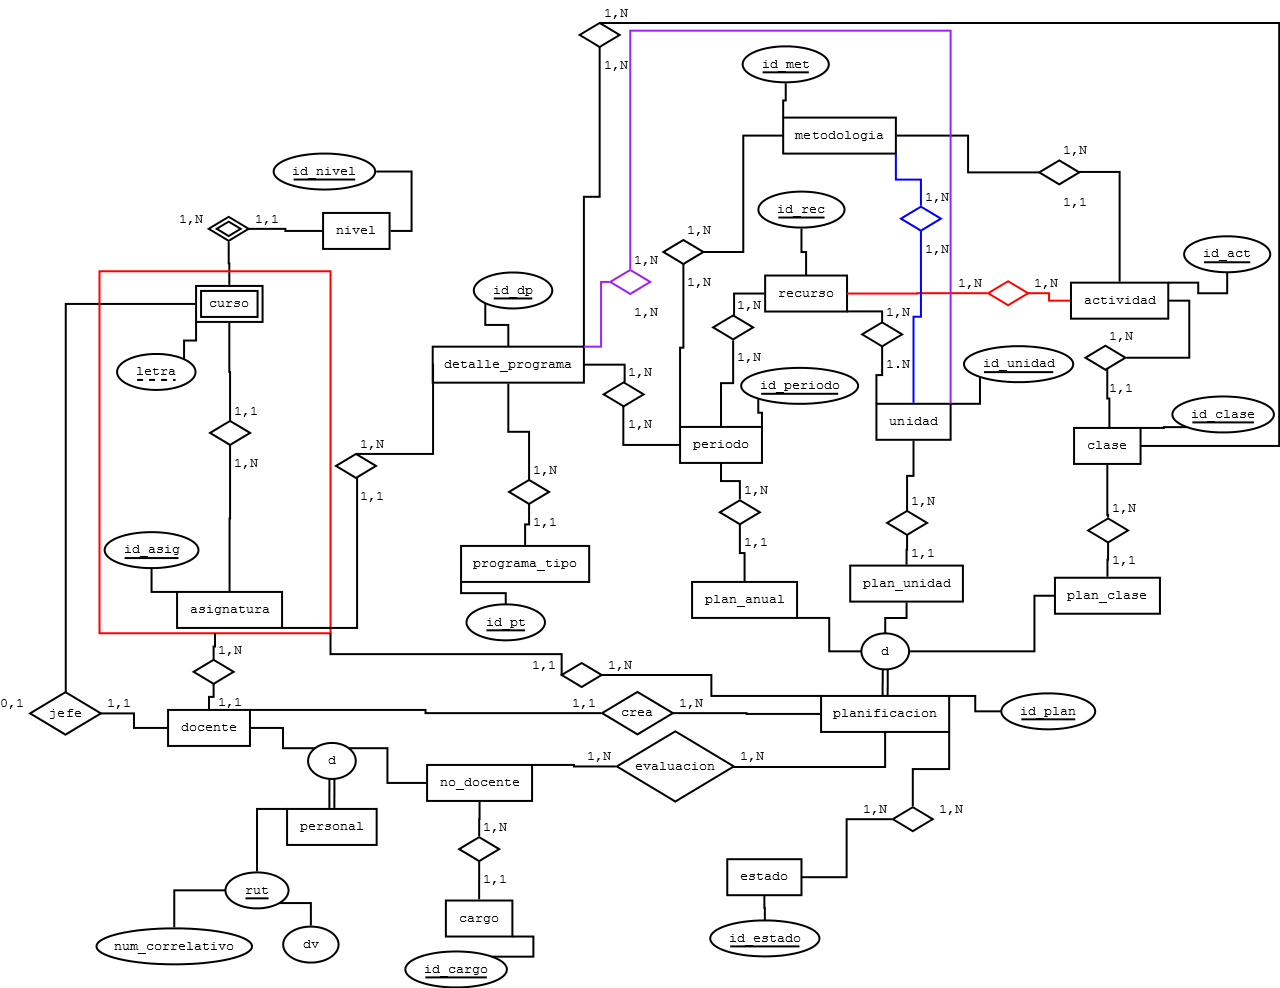
\includegraphics[scale=.51]{capitulo3/images/der2.png}%
  \end{adjustbox}
\end{figure}
%  \begin{figure}[H]
%  \begin{center}
%   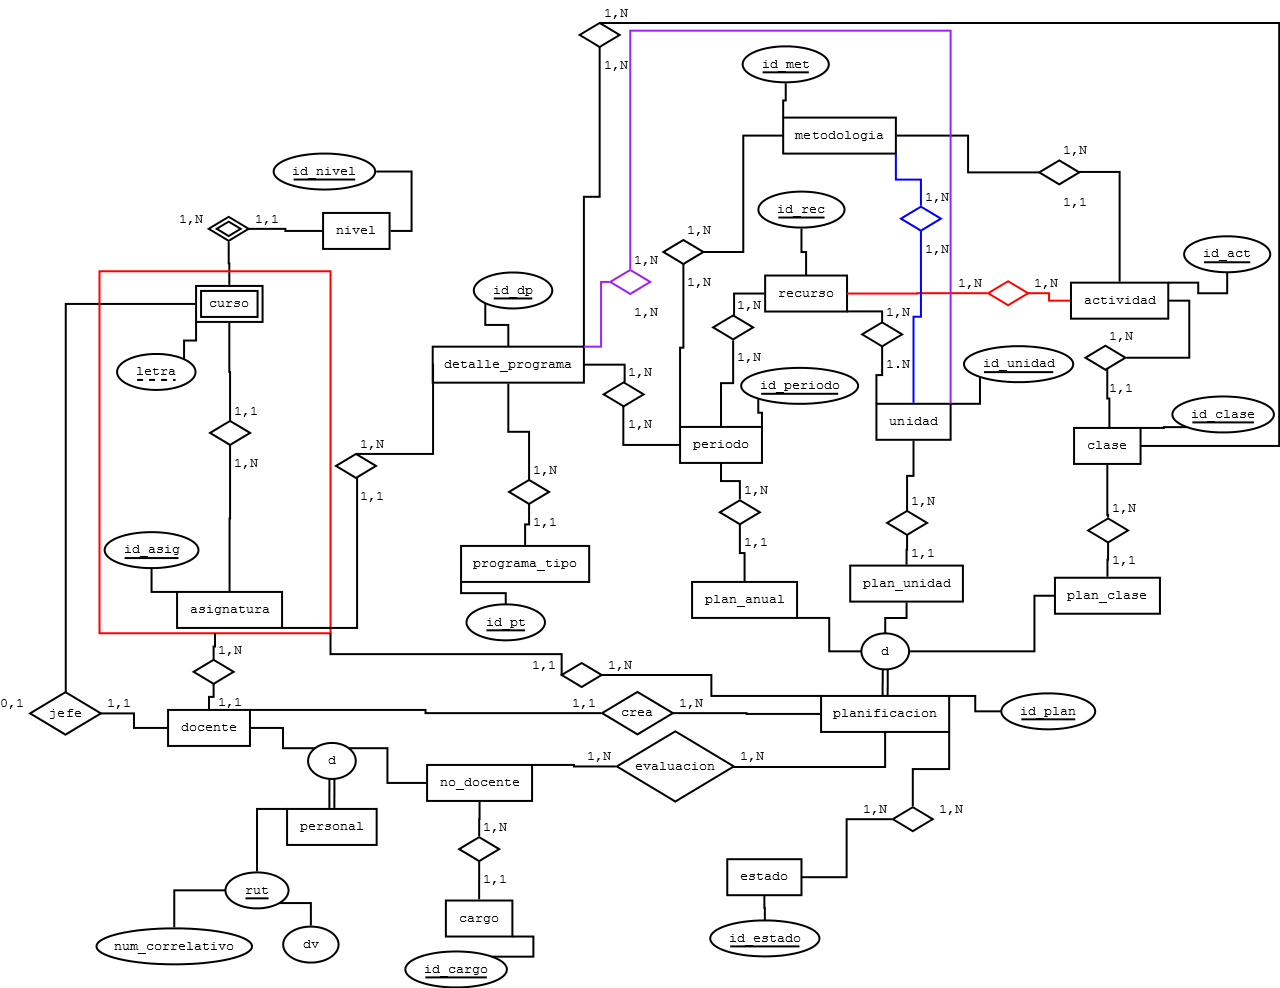
\includegraphics [scale=0.6]{capitulo3/images/der2.png} \end{center}
%  \caption{\label{Figura 31}Diagrama entidad relaci�n}
%  \end{figure}
%%%%%%%%%%%%%%%%%%%%%%%%%%%%%%%%%%%%%%%%%%%%%%%%%%%%%%%%%%%%%%%%%%

\section{Modelo relacional}

\noindent A continuaci�n se presenta el modelo relacional del caso de estudio.
Para realizar la transformaci�n del modelo entidad-relacionamiento al modelo
relacional se utiliz� la opci�n 8 a mencionada en \cite{navathe} para las especializaciones
y/o generalizaciones.

\par \noindent Los c�digos SQL DDL (Data Definition Language, por sus siglas
en ingl�s) de la implementaci�n y la documentaci�n de tablas se encuentran
detallados en el Anexo \ref{tablas} y Anexo \ref{docrelacional} respectivamente.
\\

\par 

\noindent \tn{nivel}(\underline{id\_nivel},nom\_nivel)

\noindent \tn{curso}(\underline{id\_nivel,letra},a�o,num\_correlativo,dv)

\noindent \tn{programa\_tipo}(\underline{id\_pt},nom\_pt,abrev)

\noindent
\tn{detalle\_programa}(\underline{id\_dp},nom\_dp,desc\_dp,id\_pt,id\_asig)

\noindent
\tn{personal}(\underline{num\_correlativo,dv},nombres,apaterno,amaterno,fnac,calle,num,cod\_postal,\\
\hspace{4cm}ciudad,region)

\noindent \tn{personalmail}(\underline{num\_correlativo,dv,mail})

\noindent \tn{personalcelular}(\underline{num\_correlativo,dv,celular})

\noindent \tn{docente}(\underline{num\_correlativo,dv})

\noindent \tn{no\_docente}(\underline{num\_correlativo,dv},id\_cargo)

\noindent
\tn{asignatura}(\underline{id\_asig},nom\_asig,id\_nivel,letra,num\_correlativo,dv)

\noindent \tn{cargo}(\underline{id\_cargo},nom\_c,desc\_c)

\noindent
\tn{planificacion}(\underline{id\_plan},ult\_estado,fcreacion,ult\_modif,tipo\_plan,num\_correlativo,dv,
\\
\hspace{4cm}id\_asig)

\noindent \tn{plan\_anual}(\underline{id\_plan})

\noindent \tn{plan\_unidad}(\underline{id\_plan})

\noindent \tn{plan\_clase}(\underline{id\_plan})

\noindent
\tn{periodo}(\underline{id\_periodo},duracion,mes\_ini,mes\_ter,id\_plan\_anual)

\noindent \tn{periodo\_aprevios}(\underline{id\_periodo,aprevio})

\noindent \tn{unidad}(\underline{id\_unidad},fechai,fechat,id\_plan\_unidad)

\noindent \tn{unidad\_aprevios}(\underline{id\_unidad,aprevio})

\noindent
\tn{clase}(\underline{id\_clase},duracion,dia,hi,ht,fecha,id\_plan\_clase)

\noindent \tn{clase\_aprevios}(\underline{id\_clase,aprevio})

\noindent \tn{estado}(\underline{id\_estado},nom\_estado)

\noindent \tn{planificacion\_estado}(\underline{id\_plan,id\_estado})

\noindent
\tn{planificacion\_estado\_fcambio}(\underline{id\_plan,id\_estado,fcambio})

\noindent \tn{evaluacion}(\underline{num\_correlativo,dv,id\_plan})

\noindent
\tn{evaluacion\_detalle}(\underline{num\_correlativo,dv,id\_plan,fecha\_eva},comentario)

\noindent \tn{metodologia}(\underline{id\_met},nom\_met,desc\_met)

\noindent \tn{metodologia\_unidad}(\underline{id\_met,id\_unidad})

\noindent \tn{metodologia\_periodo}(\underline{id\_met,id\_periodo})

\noindent \tn{recurso}(\underline{id\_rec},nom\_rec,desc\_rec)

\noindent \tn{recurso\_unidad}(\underline{id\_rec,id\_unidad})

\noindent \tn{recurso\_periodo}(\underline{id\_rec,id\_periodo})

\noindent \tn{recurso\_actividad}(\underline{id\_rec,id\_act})

\noindent
\tn{actividad}(\underline{id\_act},desc\_act,duracion,id\_clase,id\_met)

\noindent \tn{detalle\_programa\_unidad}(\underline{id\_dp,id\_unidad})

\noindent \tn{detalle\_programa\_periodo}(\underline{id\_dp,id\_periodo})

\noindent \tn{detalle\_programa\_clase}(\underline{id\_dp,id\_clase})

%%%%%%%%%%%%%%%%%%%%%%%%%%%%%%%%%%%%%%%%%%%%%%%%%%%%%%%%%%%%%%%%%%%%%
%  \begin{figure}[H]
%  \begin{center}
%   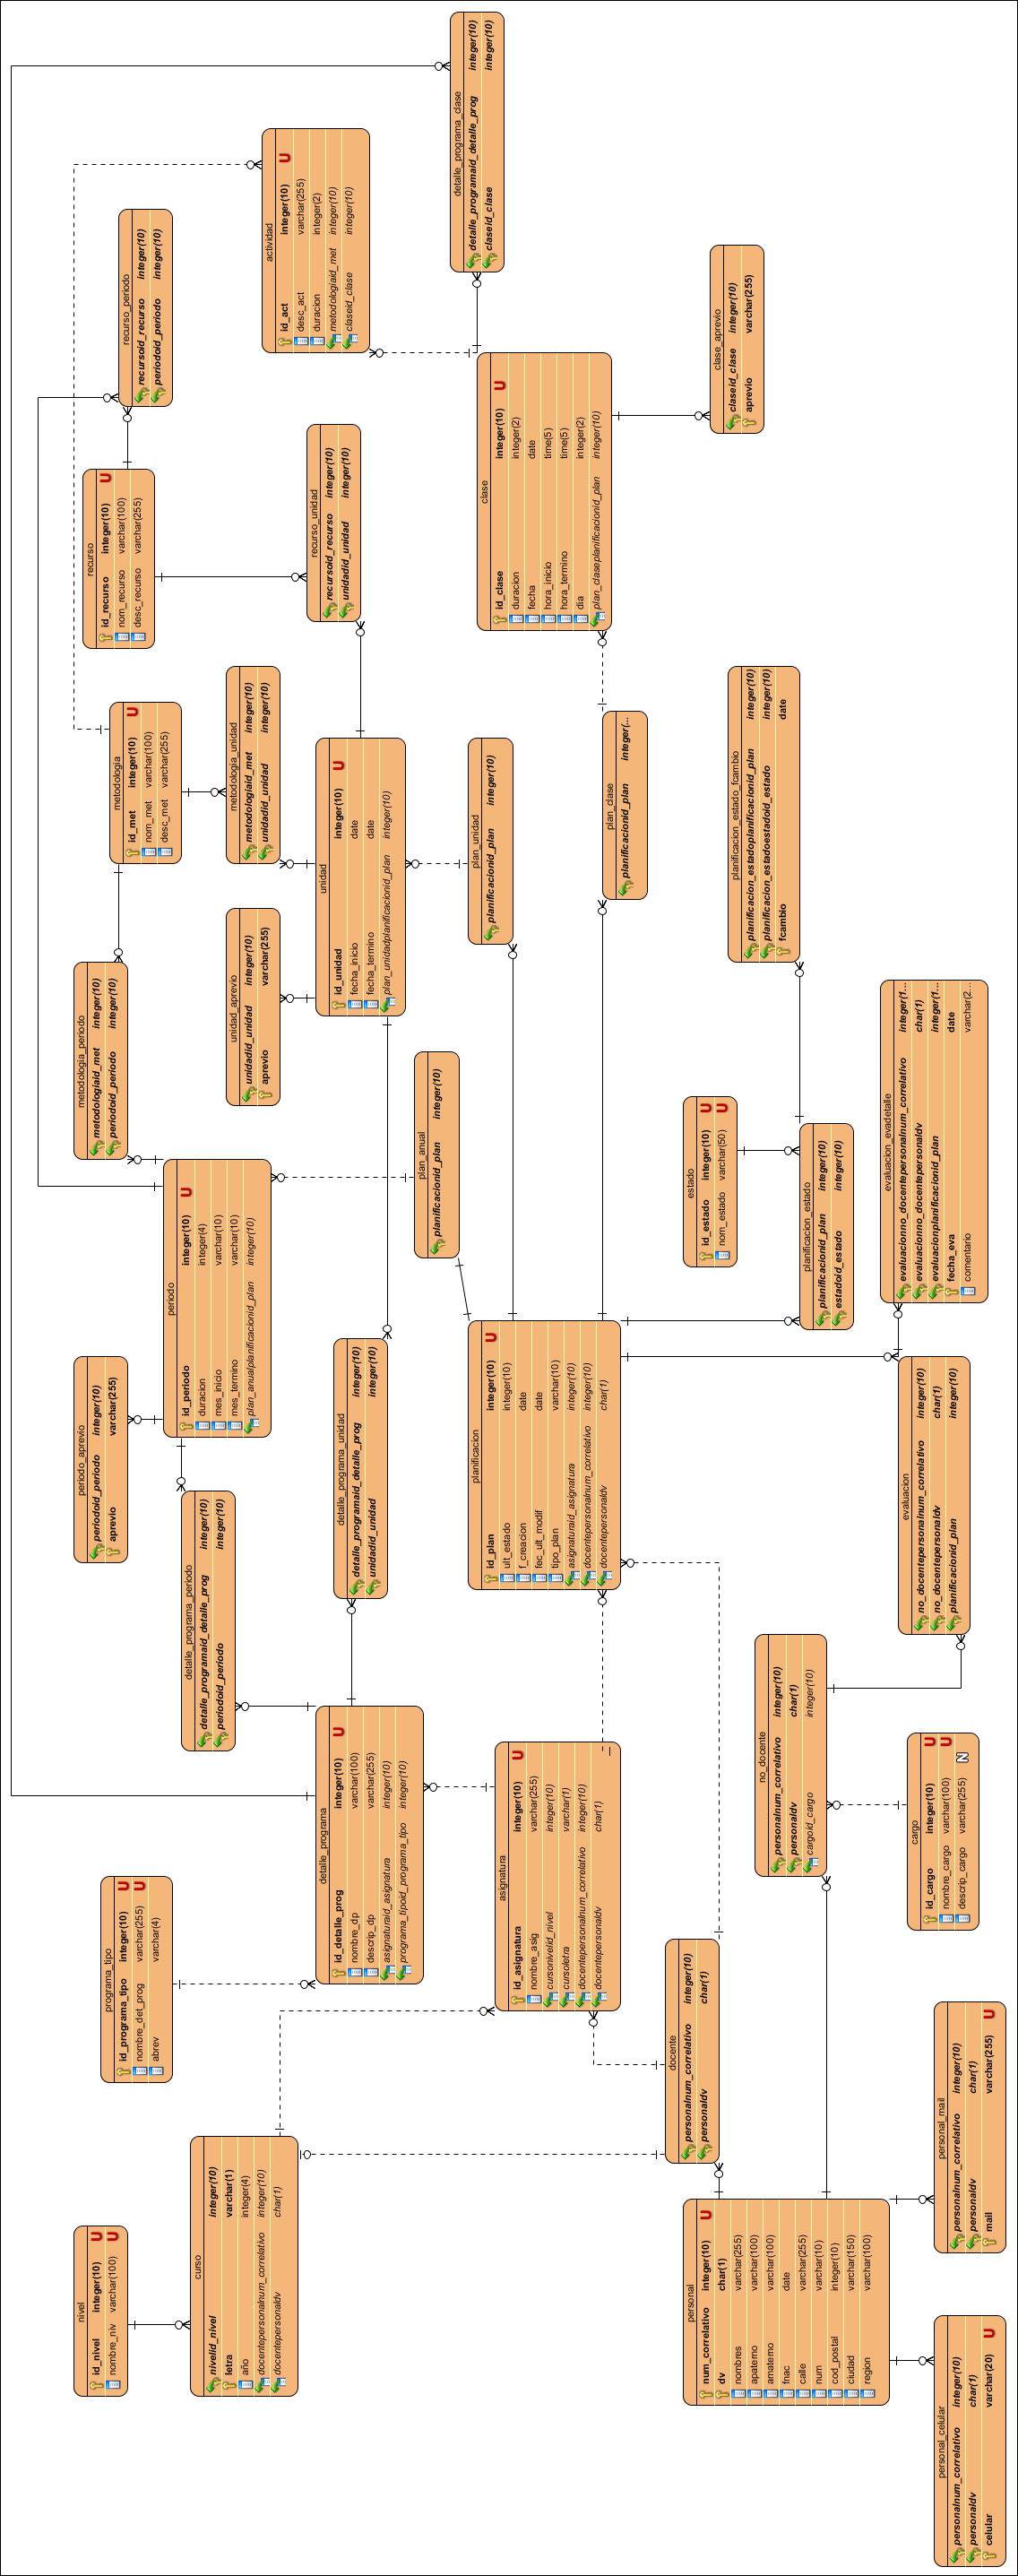
\includegraphics [scale=0.9]{capitulo3/images/mer.png} \end{center}
%  \caption{\label{Figura 32}Modelo entidad relaci�n}
%  \end{figure}
%%%%%%%%%%%%%%%%%%%%%%%%%%%%%%%%%%%%%%%%%%%%%%%%%%%%%%%%%%%%%%%%%%
\newpage
\section{Notaci�n UML para el modelo entidad relacionamiento}

\par \noindent Para un mayor entendimiento de c�mo se debe implementar el modelo
objeto relacional es importante tener una visi�n del caso de estudio en notaci�n
UML, ya que es m�s sencillo de visualizar y de transformar. Pero primero se
especificar� la representaci�n propuesta por \cite{navathe} de entidad
relacionamiento a UML.

\par \noindent En los diagramas de clase
UML, una clase (equivalente a un tipo de entidad en ER) se muestra como un
cuadro (v�ase la figura \ref{FiguraUML}) que incluye tres secciones: la secci�n
superior ofrece el nombre de la clase; la secci�n intermedia incluye los atributos de los objetos individuales 
de la clase; y la �ltima secci�n incluye las operaciones que se pueden aplicar a
esos objetos. En los diagramas ER no se especifican las operaciones.
Un atributo compuesto se modela como un dominio
estructurado. Un atributo multivaluado generalmente se modelar� como una clase
separada o como un atributo del tipo arreglo que contenga los valores.

\par \noindent En la tecnolog�a UML, los tipos de relaci�n se denominan asociaciones y las instancias de relaci�n, v�nculos. Una asociaci�n binaria (tipo de relaci�n binaria) se representa como una l�nea que conecta las clases participantes (tipos de entidad)
y, opcionalmente, puede tener un nombre. Un atributo de relaci�n, denominado
atributo de v�nculo, se coloca en un recuadro conectado con la l�nea de la asociaci�n mediante una l�nea discontinua.
La notaci�n (m�n, m�x) se utiliza para especificar las restricciones de
relaci�n, que en terminolog�a UML se denominan multiplicidades. Las multiplicidades se especifican como 
m�n .. m�x, y un asterisco (*) indica que no hay un l�mite m�ximo en la participaci�n. No obstante, las 
multiplicidades se colocan en los extremos opuestos de la relaci�n.
En UML, un asterisco indica una multiplicidad de O ..*, y un 1 indica una multiplicidad de 1..1.

\par \noindent En UML, hay dos tipos de relaciones: asociaci�n y agregaci�n. La
agregaci�n est� pensada para representar una relaci�n entre un objeto completo y sus partes constitutivas, y tiene una
notaci�n diagram�tica distinta. No obstante la agregaci�n y la asociaci�n no
tienen propiedades estructurales diferentes y la elecci�n del tipo de relaci�n que
hay que utilizar es algo subjetivo. En el modelo ER, las dos se representan
como relaciones. 

\par \noindent UML tambi�n distingue entre asociaciones (o agregaciones) unidireccionales y bidireccionales. En el caso
unidireccional,
la l�nea que conecta las clases se muestra con una flecha para indicar que s�lo se necesita una
direcci�n para acceder a los objetos relacionados. Si no aparece una flecha, se asume la cualidad bidireccional,
que es lo predeterminado. Por otro lado, para representar una entidad d�bil se
utiliza una composici�n ya que esta posee una dependencia existencial con
respecto a la entidad fuerte. En la figura \ref{FiguraUML} se muestra una
versi�n simplificada UML del caso de estudio.



%\par \noindent A continuaci�n se el c�digo SQL con la creaci�n de tablas.\\
\begin{figure}[H]
  \begin{adjustbox}{addcode={\begin{minipage}{\width}}{\caption{\label{FiguraUML}Diagrama
  UML del modelo relacional}
  \end{minipage}},rotate=90,center}
      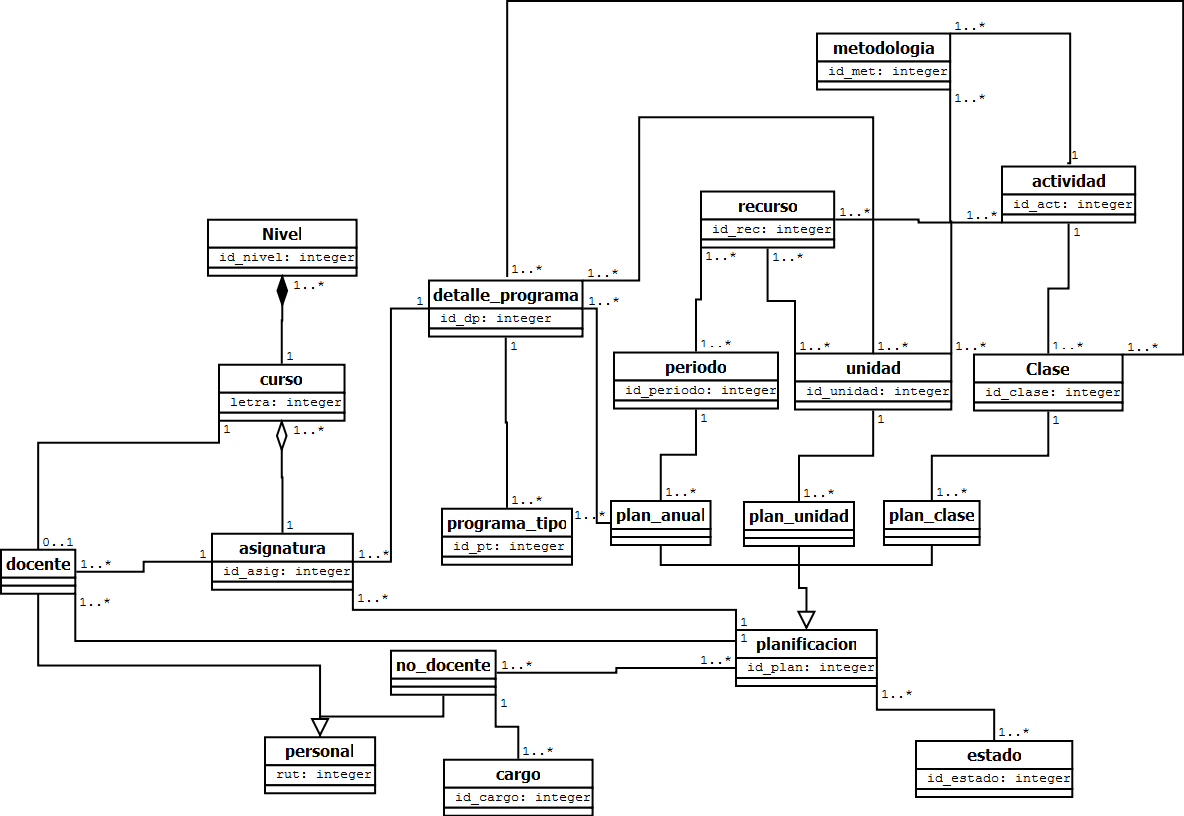
\includegraphics[scale=.5]{capitulo3/images/uml.png}%
  \end{adjustbox}
\end{figure}


\section{Implementaci�n modelo objeto relacional}

\subsection{Dise�o de una base de datos objeto relacional utilizando la
transformaci�n de ER a objeto relacional}

\par \noindent En la siguiente secci�n de presentar� una descripci�n de un
algoritmo propuesto que puede transformar un esquema ER en el esquema de una
base de datos objeto relacional.

\subsubsection{Algoritmo propuesto para la transformaci�n de ER a objeto
relacional en Oracle 11G} \label{algoritmoor}

\par \noindent A continuaci�n, se describir�n los pasos de un algoritmo para la
transformaci�n de ER en objeto relacional. Se emplear� la base de datos del caso
de estudio. El esquema ER de esta base de datos se muestra en la figura
\ref{Figura 31}, mientras que en la figura \ref{FiguraUML}  se muestra el
esquema de la base de datos objeto relacional correspondiente para ilustrar los pasos del
mapeado. \\

\par \noindent \tn{Paso 1: Mapeado de atributos compuestos}
\par \noindent Por cada
atributo compuesto \tn{C} del esquema ER, se crea un tipo
estructurado \tn{et} que contenga todos los atributos simples de \ti{C}. Los
tipos estructurados son �tiles para representar atributos compuestos cuando
dicho atributo debe ser utilizado en m�ltiples tablas o definiciones de tipos.
Por ejemplo, el atributo direcci�n que se ilustra en la figura \ref{Figurap} 
se definir� como tipo estructurado. En el c�digo \ref{acom} se ve el resultado
de la transformaci�n.

 \begin{figure}[!hbtp]
 \begin{center}
  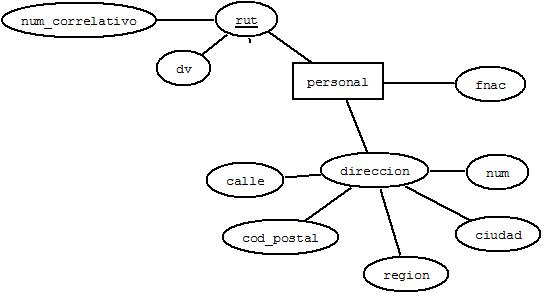
\includegraphics [scale=0.8]{capitulo3/images/Diagrama1.jpeg} \end{center}
 \caption{\label{Figurap}Entidad Personal con atributo compuesto}
 \end{figure}
 \newpage
 \begin{lstlisting}[language=SQL, caption={Definici�n de tipo estructurado para
 atributo compuesto},label=acom] 
 CREATE TYPE tDireccion AS OBJECT
 (	calle	varchar2(255), 	num		varchar2(10),
 	cod_postal	number(10),
 	ciudad		varchar2(150),
 	region		varchar2(100));
 	
 CREATE TYPE tRut AS OBJECT (	
 num_correlativo		number(10), 	dv		char(1));
 	
 CREATE TYPE tPersonal AS OBJECT
 (	rut		tRut,
 	fnac	date,  	direccion	tDireccion);
 	
 CREATE TABLE Personal OF tPersonal
 (	primary key(rut.num_correlativo, rut.dv));
\end{lstlisting}


\noindent Es preciso definir los dos casos posibles de
implementaci�n, tanto para atributos multivaluados, como para relacionamientos
de 1 : \ N y relacionamientos de N : \ M. 

\begin{itemize}
  \item En caso de que se conozca el tama�o del relacionamiento o del atributo
  multivaluado, por ejemplo: 
  \begin{itemize}
  \item Un persona tiene a lo m�s 2 tel�fonos fijos.
  \item Un alumno puede pertenecer como m�ximo a 3 carreras distintas dentro de
  la univesidad.
  \end{itemize}
  \item En el caso de no conocer el tama�o m�ximo.
\end{itemize}

\par \noindent \tn{�Qu� utilizar dependiendo del caso?}


\begin{itemize}
\item Cuando el valor m�ximo es conocido, se propone utilizar un varray para
almacenar referencias de los tipos de objetos.
\item Cuando el valor no se conoce, se utiliza tablas anidadas, donde se
almacenan referencias del tipo de objeto.
\item Existe la posibilidad de utilizar un varray aunque se desconozca el valor
m�ximo, en este caso se crea un varray con un tama�o m�ximo de tope a criterio
del programador. Para realizar la manipulaci�n de datos, es necesario crear
procedimientos almacenados o m�todos dentro del objeto que sean capaces de
verificar si el varray tiene espacio disponible para insertar nuevos datos.
	
\end{itemize}

\noindent Sin embargo, la propuesta anterior que en teor�a es la soluci�n
correcta para cualquier caso, si el problema es muy complejo y las entidades poseen
una gran cantidad de relacionamientos Oracle, no permite su correcto
funcionamiento y a la vez mantener la navegabilidad bidireccional.
Por este motivo para los relacionamientos 1 a N se utilizar� la opci�n de crear
un varray con un tama�o m�ximo a criterio.
En el caso de un relacionamiento de N a N se propone crear un nuevo tipo
objeto intersecci�n, el cual posee una referencia a cada objeto con el que se
tiene un relacionamiento, para luego crear un listado (varray) de referencias a ese nuevo objeto intersecci�n y es dicho
 listado el que se agrega a cada objeto del relacionamiento. En la figura
 \ref{nn1} y figura \ref{nn2} se muestra un ejemplo del tipo intersecci�n y el
 listado de referencias.
  
\begin{figure}[H]
 \begin{center}
  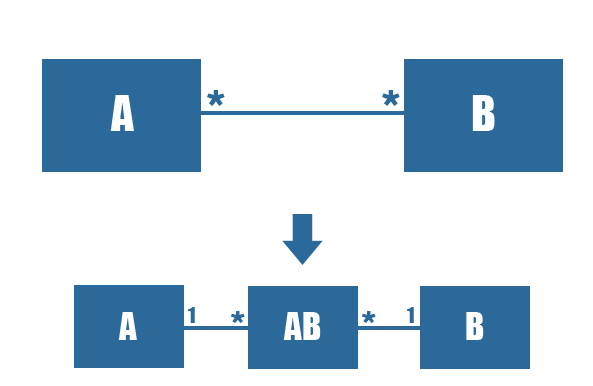
\includegraphics [scale=0.65]{capitulo3/images/nn1.png}
  \end{center}
 \caption{\label{nn1}Ejemplo objetos relacionamiento N : N}
 \end{figure} 
 
 \begin{figure}[H]
 \begin{center}
  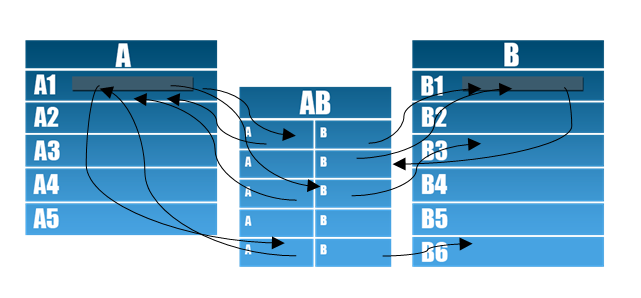
\includegraphics [scale=0.6]{capitulo3/images/nn2.png}
  \end{center}
 \caption{\label{nn2}Ejemplo objeto intersecci�n relacionamiento N : N}
 \end{figure}

\noindent Para el caso de estudio ser�
implementado con navegabilidad bidireccional por requerimiento del profesor gu�a, ya que cualquier objeto
debe conocer con quien se encuentra asociado. 

\noindent Cabe destacar, que desde el est�ndar SQL 2003 se tiene soporte a
MULTISET para reemplazar a los arreglos y es la forma en c�mo se implementan los
relacionamientos en dicho est�ndar \cite{transformacion_or}. En la tabla
\ref{tablasql_oracle} se presenta la diferencia entre Oracle y el est�ndar 2003.

\begin{table}[H]
\begin{center}
\begin{tabular}{|l|p{4cm}|p{5cm}|}
 \hline
\tn{Modelo conceptual}      & \tn{Est�ndar SQL:2003}       & \tn{Oracle}                                              
\\ \hline Clase & Tipo estructurado		& Tipo Objeto                             
\\ \hline Extensi�n de clase       & Tabla Tipada	& Tabla de Tipo Objeto                                            
\\ \hline Atributo Multivaluado  & Array / Multiset	&	Varray/Nested Table
\\ \hline Atributo Compuesto 	&	Row / Columna de Tipo Estructurado	& Columna de
Tipo Objeto 
\\	\hline Atributo Derivado	&	Trigger/M�todo		& Trigger/M�todo
\\ \hline	Asociaci�n 1 : 1	& Ref / Ref		&	Ref / Ref
\\ \hline	Asociaci�n 1 : N	& Ref / Multiset / Array		&	Ref /
Nested Table / Varray
\\ \hline	Asociaci�n N : M	& Multiset / Multiset o Array / Array	& Nested
Table / Nested Table o Varray / Varray
\\ \hline Asociaci�n Agregaci�n		& 	Multiset / Array	& Nested Table / Varray de
Referencias
\\ \hline Asociaci�n Composici�n	&  Multiset / Array	& Nested Table / Varray de
Objetos
\\ \hline	Asociaci�n Generalizaci�n	& Tipos / Tablas Tipadas	& Tipos / Tablas de
Tipo Objeto. \\ 
\hline
\end{tabular}
\caption[Reglas de transformaci�n a Modelo Objeto
relacional]{\label{tablasql_oracle}Reglas de transformaci�n (Modelo conceptual - Modelo Objeto relacional) \cite{transformacion_or}}

\end{center}
\end{table}


\par \noindent \tn{Paso 2: Mapeado de atributos multivaluados} 
\par \noindent Por cada atributo multivaluado del esquema ER, existen dos m�todos para realizar el
mapeado: s� el tama�o del atributo multivaluado es conocido \ti{MV} y s� se
desconoce el tama�o del atributo \ti{MT}. Para \ti{MV} se puede representar
directamente como un atributo de un tipo objeto \tn{et} para la tabla de
tipos \tn{c}, en donde se define un varray \tn{V} de referencias de un tipo de
datos espec�fico. Si es un atributo multivaluado compuesto, crear un \tn{V} que
contenga un tipo estructurado con los atributos simples de \ti{MV}.
Por ejemplo en el atributo celular que se ilustra en la figura \ref{Figuram},
 definir� como tipo varray, se supondr� que a lo m�s se almacenar�n 5 n�meros,
 en el c�digo
\ref{amul} se ve el resultado de la transformaci�n. 

\begin{figure}[!hbtp]
 \begin{center}
  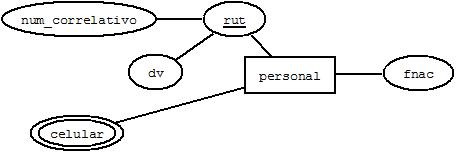
\includegraphics [scale=1]{capitulo3/images/Diagrama2.jpeg}
  \end{center}
 \caption{\label{Figuram}Entidad Personal con atributo multivaluado}
 \end{figure}
% \newpage
 \begin{lstlisting}[language=SQL, caption={Definici�n de tipo varray para
 atributo multivaluado},label=amul]
 CREATE TYPE tCelular AS OBJECT ( num_celular	number(20));
 CREATE TYPE Celulares AS VARRAY(5) OF REF tCelular;
 CREATE TYPE tRut AS OBJECT ( num_correlativo	number(10), dv	char(1));
 
 CREATE TYPE tPersonal AS OBJECT
 (	rut		tRut,
 	fnac	date,
 	celular	Celulares);
 	
 CREATE TABLE Personal OF tPersonal
 (	primary key(rut.num_correlativo,rut.dv));
\end{lstlisting}

\par \noindent \tn{Paso 3: Mapeado de atributos derivados}
\par \noindent Por cada atributo derivado \ti{D} del esquema ER, se define como
un m�todo en el tipo estructurado \tn{et} que realice el c�lculo requerido y devuelva su valor.
Por ejemplo en el atributo edad que se ilustra en la figura \ref{Figurad}, se
definir� como m�todo. En el c�digo \ref{ader} se ve el resultado
de la transformaci�n.

\begin{figure}[H]
 \begin{center}
  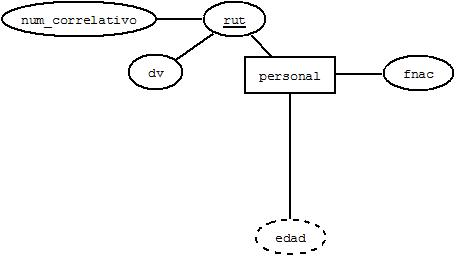
\includegraphics [scale=0.8]{capitulo3/images/Diagrama3.jpeg}
  \end{center}
 \caption{\label{Figurad}Entidad Personal con atributo derivado}
 \end{figure}
 
  \begin{lstlisting}[language=SQL, caption={Definici�n de m�todo para
 atributo derivado},label=ader]
 CREATE TYPE tRut AS OBJECT (num_correlativo	number(10), dv	char(1));
 CREATE TYPE tPersonal AS OBJECT
 (	rut		tRut, 	fnac	date,
 	MEMBER FUNCTION edad RETURN NUMBER)
 / 	
 CREATE TYPE BODY tPersonal IS
  MEMBER function edad RETURN NUMBER IS
    BEGIN
     return(trunc(months_between(Sysdate, self.fnac) / 12));
    END;
  END;  /
  
 CREATE TABLE Personal OF tPersonal
 (	primary key(rut.num_correlativo, rut.dv));
\end{lstlisting}

\par \noindent \tn{Paso 4: Mapeado de los tipos de relaci�n 1:1
binaria}
\par \noindent Por cada tipo de relaci�n 1:1 binaria \tn{R} sin atributos del
esquema ER, identifique las relaciones \tn{S} y \tn{T} que corresponden a los tipos de
entidad que participan en \tn{R}. Se define una tabla de tipos \tn{S1} que posee un tipo estructurado \tn{s1t} con un atributo de tipo
referencia (t1t). Adem�s definir un tabla de tipos \tn{T1} que posee un tipo
estructurado \tn{t1t} con un atributo de tipo referencia (s1t).\\

\par \noindent \tn{Paso 5: Mapeado de tipos de relaciones 1:N
binarias}
\par \noindent Por cada relaci�n 1:N binaria regular \tn{R} sin atributos,
identifique la relaci�n \tn{S} que representa el tipo de entidad participante en el lado N del tipo de relaci�n. 
Al igual que en el mapeado de los tipos de relaci�n 1:1 sin atributos, se define una tabla de tipos \tn{b}
que posee un tipo objeto \tn{bt} con un atributo del tipo Varray
que contiene referencias del tipo objeto del lado N. Por ejemplo en el
relacionamiento que se ilustra en la figura \ref{Figurad1}, se definir�n los
tipos tActividad y tMetodologia, en donde tActividad tiene una referencia a la
metodolog�a que utiliza, en cambio para representar las actividades que han
utilizado cierta metodolog�a se emplea un Varray que almacena
referencias de dichas actividades. En el c�digo \ref{n1} se ve el resultado de
la transformaci�n.

\begin{figure}[H]
 \begin{center}
  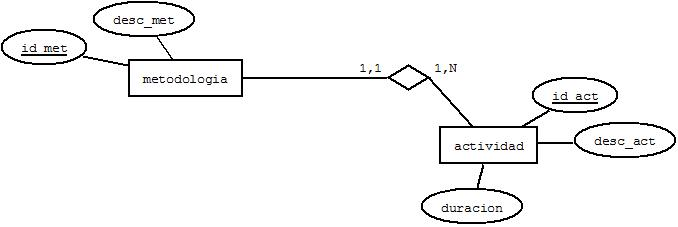
\includegraphics [scale=0.8]{capitulo3/images/Diagrama4.jpeg}
  \end{center}
 \caption{\label{Figurad1}Relacionamiento 1 a N}
 \end{figure}


  \begin{lstlisting}[language=SQL, caption={Definici�n de tipos para
 relacionamiento 1 a N},label=n1]
  CREATE TYPE tActividad AS OBJECT (	
 id_act		varchar2(10), 	
 desc_act	varchar2(255),
 duracion	integer, 	
 met_usada	REF metodologia);
 	
 CREATE TYPE ListadoActividades AS VARRAY(50) OF REF tActividades;
 
 CREATE TABLE Actividad OF tActividad (PRIMARY KEY (id_act));
 	 	
 CREATE TYPE tMetodologia AS OBJECT
 (id_met	varchar2(10), 
 desc_met	varchar2(255), 
 actividades	ListadoActividades); 
 
 CREATE TABLE Metodologia OF tMetodologia 
 (PRIMARY KEY	(id_met));
\end{lstlisting}

\par \noindent \tn{Paso 6: Mapeado de tipos de relaciones M:N
binarias}
\par \noindent Por cada tipo de relaci�n M:N binaria \tn{R} sin atributos, se
 debe definir un atributo del tipo objeto \tn{to} que contiene referencias del
 tipo objeto M y del tipo objeto N. Se le debe agregar a cada tipo objeto un
 varray de referencias del tipo \tn{to}, para luego crear una nueva tabla
 \tn{tt} de tipos \tn{to}.
 
 \noindent En caso de que  \tn{R} tenga atributos se debe crear una nueva tabla
 de tipo \tn{S} para representar a \tn{R}. La tabla de relaci�n \tn{S} incluye un tipo objeto \tn{to} que contiene referencias de cada tipo objeto de
 la tabla de tipo correspondiente, que participa en la relaci�n y adem�s los atributos que
 posea la relaci�n, al igual que en el relacionamiento sin atributos, a cada
 objeto se le debe agregar un atributo varray con referencias al tipo objeto
 \tn{to}.
 
 \noindent Por ejemplo en el relacionamiento que se ilustra en la figura
 \ref{Figurae}, se definir�n los tipos tActividad y tRecurso, en donde se crea el tipo objeto y luego una tabla que almacena referencias de actividades y recursos. En el c�digo \ref{nn} se ve el resultado de la transformaci�n. Otro ejemplo se
visualiza en la figura \ref{Figuranna}, donde existe un relacionamiento M:N con
atributos, en el c�digo \ref{nna} se ve el resultado de su implementaci�n. \\

\hspace{6cm}

\begin{figure}[H]
 \begin{center}
  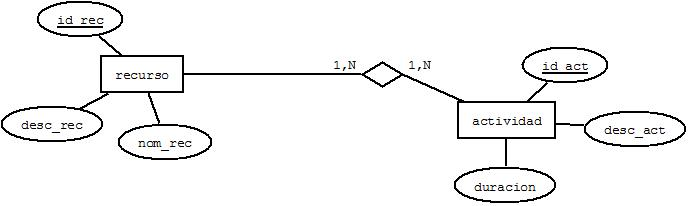
\includegraphics [scale=0.8]{capitulo3/images/Diagrama5.jpeg}
  \end{center}
 \caption{\label{Figurae}Relacionamiento N a N}
 \end{figure}
 
 \newpage 
 
  \begin{lstlisting}[language=SQL, caption={Definici�n de tipos para
 relacionamiento N a N},label=nn] 
  CREATE TYPE tActividad AS OBJECT (	
  id_act		varchar2(10), desc_act	varchar2(255),
 	duracion	integer,); 
 
 CREATE TYPE tRecurso AS OBJECT (	
 	id_rec		varchar2(10), nom_rec	varchar2(100),
 	desc_rec	varchar2(255)); 
 	
 CREATE TYPE Trecurso_actividad AS OBJECT(
 actividad	REF tActividad, recurso		REF tRecurso); 
 
 CREATE TYPE listado_recurso_activdad AS VARRAY(50) OF REF Trecurso_actividad;
 
 ALTER TYPE tRecurso ADD ATTRIBUTE (listado_actividades
 listado_recurso_actividad) CASCADE;
 
 ALTER TYPE tActividad ADD ATTRIBUTE (listado_recursos
 listado_recurso_actividad) CASCADE;
 
 CREATE TABLE Actividad OF tActividad (	PRIMARY KEY (id_act)); /
 
 CREATE TABLE Recurso OF tRecurso ( PRIMARY KEY (id_rec)); /
 
 CREATE TABLE Recurso_Activadad OF Trecurso_activadad (
 PRIMARY KEY (actividad.id_act,recurso.id_rec));
\end{lstlisting}

\begin{figure}[H]
 \begin{center}
  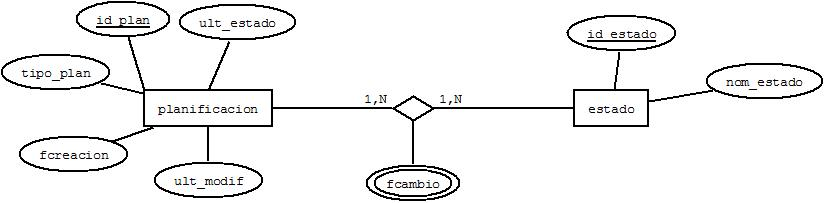
\includegraphics [scale=0.7]{capitulo3/images/Diagrama5_1.jpeg}
  \end{center}
 \caption{\label{Figuranna}Relacionamiento N a N con atributos}
 \end{figure}
 

  \begin{lstlisting}[language=SQL, caption={Definici�n de tipos para
 relacionamiento N a N con atributos},label=nna] 
  CREATE TYPE tPlanificacion AS OBJECT (
  id_plan		varchar2(10),
 	tipo_plan	varchar2(10),
 	fcreacion	date,
 	ult_estado	varchar2(10),
 	ult_modif	varchar2(10)); 
 
 CREATE TYPE tEstado AS OBJECT (
 	id_estado	varchar2(10),
 	nom_estado	varchar(50)); 
 
 CREATE TYPE fcambio AS OBJECT (
 	fecha_cambio	date)); 
 
 CREATE TYPE fecha_cambio AS VARRAY(10) OF fcambio; 
 
 CREATE TYPE tPlanificacion_Estado_fcambio AS OBJECT (
  planificacion	ref tPlanificacion,
 	estado		ref tEstado,
 	fecha_c		fecha_cambio); 
 	
 CREATE TYPE listado_planificacion_estado AS VARRAY(50) OF REF
 tPlanificacion_Estado_fcambio;
 
 ALTER TYPE tPlanificacion ADD ATTRIBUTE (listado_estados
 listado_planificacion_estado) CASCADE;
 
 ALTER TYPE tEstado ADD ATTRIBUTE (listado_planificaciones
 listado_planificacion_estado) CASCADE;
 
 CREATE TABLE Planificacion OF tPlanificacion
 (PRIMARY KEY (id_plan)); 
  
 CREATE TABLE Estado OF tEstado
 (PRIMARY KEY (id_estado); 
 
 CREATE TABLE Planificacion_Estado OF 
 tPlanificacion_Estado_fcambio (PRIMARY KEY 
 (planificacion.id_plan,estado.id_estado));/ 
 
\end{lstlisting}


\par \noindent \tn{Paso 7: Mapeado de tipos de relaciones N arias}
\par \noindent Por cada tipo de relaci�n N aria \tn{R}, se debe crear una nueva
tabla de tipo \tn{S} para representar a \tn{R}. La tabla de relaci�n \tn{S} existen N atributos con tipo referencia definidos, uno para el
tipo objeto de cada tabla de tipo que participa en la relaci�n.
\newpage

\par \noindent \tn{Paso 8: Mapeado de tipos de relaciones
recursivas}
\par \noindent Se debe tratar como cualquier relacionamiento.
\\

\par \noindent \tn{Paso 9: Mapeado de los tipos de entidad
regulares}
\par \noindent Por cada entidad (fuerte) regular E del esquema ER, se define una
tabla de tipos \tn{S1} que posee un tipo objeto \tn{s1t} que incluya
todos los atributos simples, compuestos, multivalor y derivados de E. Un ejemplo se puede visualizar
en la figura \ref{Figurap} y su implementaci�n en el c�digo \ref{acom}.\\

\par \noindent \tn{Paso 10: Mapeado de los tipos de entidad d�biles}
\par \noindent Por cada tipo de entidad d�bil W del esquema ER con el tipo de
entidad propietario E, crear una tabla de tipo objeto para W con una clave
compuesta que incluya la clave de la tabla tipo objeto de su propietario E. El
tipo objeto para la tabla de tipo de W puede adem�s incluir un atributo del tipo
referencia que contiene una fila de la tabla de tipo que representa a E. Para el ejemplo
de la figura \ref{Figuradeb} se definir�n los tipos estructurados nivel\_ob y
curso\_ob, luego se define el varray de tipos con referencias a curso que contiene los N cursos que posee el nivel. En el c�digo
\ref{entidaddebil} se detalla la implementaci�n completa.

\begin{figure}[H]
 \begin{center}
  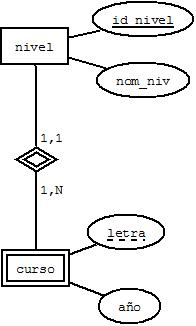
\includegraphics [scale=0.6]{capitulo3/images/Diagrama7.jpeg}
  \end{center}
 \caption{\label{Figuradeb}Entidad d�bil}
 \end{figure}

\newpage
  \begin{lstlisting}[language=SQL, caption={Definici�n de tipos para
 definici�n de entidad debil},label=entidaddebil]
 CREATE TYPE nivel_ob AS OBJECT
  ( id_nivel  NUMBER(10),
    nom_nivel varchar2(255));
    
  CREATE TYPE curso_ob AS OBJECT
  ( refnivel REF nivel_ob,
  	id_nivel NUMBER(10),
    letra CHAR(1),
    year_ DATE );
    
  CREATE TYPE Listado_Cursos AS VARRAY(50) OF REF curso_ob;
  
  ALTER TYPE nivel_ob ADD ATTRIBUTE (cursos Listado_Cursos) CASCADE;
    
  CREATE TABLE nivel OF nivel_ob ( 
  PRIMARY KEY (ID_NIVEL)); 
  
  CREATE TABLE curso OF curso_ob ( 
  id_nivel SCOPE IS NIVEL,
  PRIMARY KEY (id_nivel,letra));
  
\end{lstlisting}

\par \noindent \tn{Paso 11: Mapeado de la especializaci�n o
generalizaci�n}
\par \noindent Para mapear una cierta cantidad de subclases que juntas forman
una especializaci�n (o, alternativamente, que est�n generalizadas en una subclase), como las subclases
{PLAN\_ANUAL, PLAN\_UNIDAD,
PLAN\_CLASE} de PLANIFICACION de la figura \ref{FiguraH}. Se debe convertir cada
especializaci�n con \tn{M} subclases \{S1, S2,\ldots, Sm\} y la superclase
(generalizada) \tn{C}, en donde se debe definir un tipo objeto \tn{Ct}
para la superclase \tn{C} y luego definir \tn{M} tipos objetos \tn{S\_t}
de las subclases indicando que se heredan de la superclase \tn{Ct}. En el c�digo
\ref{her_1} se detalla el proceso de definici�n y se visualiza el resultado de la transformaci�n.

\begin{figure}[H]
 \begin{center}
  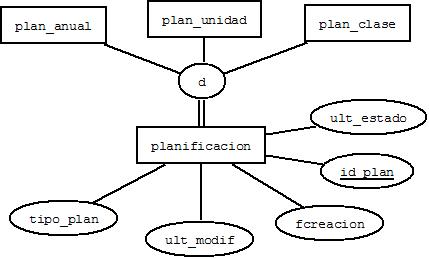
\includegraphics [scale=0.7]{capitulo3/images/Diagrama6.jpeg}
  \end{center}
 \caption{\label{FiguraH}Generalizaci�n de entidades}
 \end{figure}
 
  \begin{lstlisting}[language=SQL, caption={Definici�n de tipos para
 generalizaci�n},label=her_1]
  CREATE TYPE tPlanificacion AS OBJECT
 (	id_plan		varchar2(10),
 	tipo_plan	varchar2(10),
 	fcreacion	date,
 	ult_estado	varchar2(10),
 	ult_modif	varchar2(10))
 	NOT FINAL
 /
 CREATE TABLE Planificacion OF tPlanificacion
 (PRIMARY KEY (id_plan))
  /	 	
 CREATE TYPE tPlan_anual UNDER tPlanificacion(); /
 CREATE TYPE tPlan_unidad UNDER tPlanificacion(); /
 CREATE TYPE tPlan_clase UNDER tPlanificacion(); /
\end{lstlisting}

\par \noindent \tn{Paso 12: Mapeado de agregaciones}
\par \noindent Para mapear una agregaci�n depender� netamente de las entidades y
relacionamientos en su interior. Si por ejemplo la agregaci�n es como la de
figura \ref{figagregacion} (la cual se cambi� del problema original, para hacer
m�s sencilla la implementaci�n del ejemplo) se debe tratar como un
relacionamiento 1 : N y su implementaci�n se detalla en el c�digo \ref{agre1}.
En el caso de que el relacionamiento de la figura \ref{figagregacion} sea M : N
o 1 : 1 ver los c�digos \ref{agre2} y \ref{agre3} respectivamente.

\begin{figure}[H]
 \begin{center}
  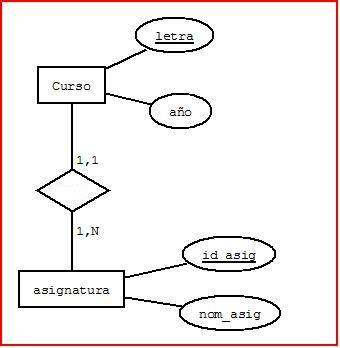
\includegraphics [scale=1.1]{capitulo3/images/Diagrama9.jpeg}
  \end{center}
 \caption{\label{figagregacion}Agregaciones}
 \end{figure}
 
 \newpage
  \begin{lstlisting}[language=SQL, caption={Definici�n de tipos
  Agregaciones con relacionamiento 1 : N},label=agre1]
CREATE TYPE curso_ob AS OBJECT  (letra CHAR(1), year_ DATE ));
    
CREATE TYPE asignatura_ob AS OBJECT (id_asig number(10),
	nom_asig	varchar2(255), 	curso_dicta	ref	curso_ob);
 	
CREATE TYPE listado_asignaturas AS VARRAY(50) OF REF asignatura_ob;

ALTER TYPE curso_ob ADD ATTRIBUTE (asignaturas	listado_asignaturas) CASCADE;
 
CREATE TABLE curso OF curso_ob ( PRIMARY KEY (letra));

CREATE TABLE asignatura OF asignatura_ob (PRIMARY KEY (id_asig)); 
\end{lstlisting}
%%%%
\\

  \begin{lstlisting}[language=SQL, caption={Definici�n de tipos
  Agregaciones con relacionamiento M : N},label=agre2]
CREATE TYPE curso_ob AS OBJECT (letra CHAR(1), year_ DATE )) /
    
CREATE TYPE asignatura_ob AS OBJECT (	
id_asig	number(10),	nom_asig  varchar2(255));
 	
CREATE TYPE curso_asignatura AS OBJECT (
curso 	ref curso_ob, asignatura  ref asignatura_ob);
 	
CREATE TYPE listado_cursos_asignaturas AS VARRAY(100) 
OF curso_asignatura;
 
ALTER TYPE curso_ob ADD ATTRIBUTE  (
asignaturas	listado_cursos_asignaturas) CASCADE;
 
ALTER TYPE asignatura_ob ADD ATTRIBUTE  (
cursos listado_cursos_asignaturas) CASCADE;
 
CREATE TABLE curso OF curso_ob ( PRIMARY KEY (letra));

CREATE TABLE asignatura OF asignatura_ob (PRIMARY KEY (id_asig)); 
\end{lstlisting}

%%%%%%
\\

  \begin{lstlisting}[language=SQL, caption={Definici�n de tipos
  Agregaciones con relacionamiento 1 : 1},label=agre3]
 CREATE TYPE curso_ob AS OBJECT
  ( letra CHAR(1),
    year_ DATE ));
    
 CREATE TYPE asignatura_ob AS OBJECT
 (	id_asig		number(10),
 	nom_asig	varchar2(255),
 	curso_dicta	ref	curso_ob);
 	  
 ALTER TYPE curso_ob ADD ATTRIBUTE (asignatura REF asignatura_ob) CASCADE;
 
CREATE TABLE curso OF curso_ob ( PRIMARY KEY (letra));

CREATE TABLE asignatura OF asignatura_ob (PRIMARY KEY (id_asig)); 
\end{lstlisting}

\subsection{Restricciones del problema para su implementaci�n}

\par \noindent Se definir�n algunas restricciones para presentar las distintas
versiones de implementar el caso de estudio en el modelo objeto relacional. Ya
que al conocer el tama�o exacto de cada relacionamiento se hace m�s sencilla su
implementaci�n.

\par \noindent Las restricciones son las siguientes: 

\begin{itemize}
  \item Cada personal a lo m�s tendr� 5 celulares y mails asociados.
  \item Cada periodo, unidad y clase a lo m�s tendr� 10 aprendizajes previos
  asociados.
  \item Cada actividad de una clase utiliza a lo m�s 3 metodolog�as educativas.
  \item Cada clase a lo m�s puede realizar 5 actividades.
\end{itemize}

\par \noindent Los c�digos SQL DDL (Data Definition Language) de los tipos y
tablas de tipos se encuentran detallados en el Anexo
\ref{tipos_or} y \ref{tablas_or} respectivamente.

 \section{Implementaci�n de modelo de datos semi estructurado}
 
 \par \noindent Primero se extrajo una parte del caso de
 estudio, para luego modificarlo o agregarle un nuevo requerimiento con el
 prop�sito de lograr realizar una implementaci�n apropiada del problema
 utilizando datos semi estructurados.
 
 \par \noindent En esta secci�n se pretende realzar la utilidad de emplear
 los datos semi estructurados en conjunto con el modelo objeto relacional en
 Oracle, para esto se presentar�n algunos ejemplos representados en el caso de
 estudio, para as� ver la real ganancia en problemas del mundo real.
 
 \subsection{Nuevo requerimiento}
 \par \noindent Para el caso de estudio descrito con anterioridad, es necesario almacenar la informaci�n educacional (establecimientos donde cada
 persona ha estudiado), idiomas que este domina y cursos de
 perfeccionamiento que haya realizado cada personal del establecimiento, con el
 fin de disponer de mayor informaci�n curricular  de cada empleado.
 Dado a lo anterior, se agregar� un atributo curr�culum a cada personal,
 con el prop�sito de almacenar dicha informaci�n. 
 
 \noindent Como la informaci�n curricular  de cada persona var�a, ya sea por la
 profesi�n o la cantidad de estudios que este posea, se sugiere  utilizar las
 capacidades de XML dentro de Oracle como la soluci�n m�s viable para almacenar
 dicha informaci�n semi estructurada.
 Para lograr este objeto, el nuevo atributo curr�culum deber� ser del tipo
 XMLType. 
 
 \noindent La estructura de cada documento XML ingresado en dicha columna debe
 ser validado previamente. En el anexo \ref{anexo_xml} se presenta en detalle el
 proceso de validaci�n y registro de esquema en Oracle.
 
 \noindent En el c�digo \ref{codigoxml_1} se muestra el esquema XML del
 curr�culum de una persona, el cual ha sido registrado en Oracle mediante la
 funci�n DBMS\_XMLSCHEMA. 
 
\noindent En el c�digo \ref{ejemxml1} se muestra c�mo utilizar una columna del
tipo XML que contiene todos los datos del curr�culum de una persona dentro de un
tipo objeto. Luego en el c�digo \ref{ejemxml2} se realiza una inserci�n en la
tabla personal\_ob2\_xml, con el fin de efectuar futuras pruebas de selecci�n,
actualizaci�n y eliminaci�n en tablas con columnas XMLType.
 
  \newpage
 \begin{lstlisting}[language=xml, caption={Ejemplo de estructura del
 curr�culum}, label=codigoxml_1] 
<xs:schema attributeFormDefault="unqualified" elementFormDefault="qualified" 
xmlns:xs="http://www.w3.org/2001/XMLSchema">
  <xs:element name="curriculum">
    <xs:complexType><xs:sequence>
        <xs:element name="estudios"><xs:complexType><xs:sequence>
              <xs:element name="estudio" maxOccurs="unbounded" minOccurs="0">
                <xs:complexType><xs:sequence>
                    <xs:element type="xs:string" name="nombre_establecimiento"/>
                    <xs:element type="xs:string" name="carrera" minOccurs="0"/>
                    <xs:element type="xs:string" name="ciudad"/>
                    <xs:element type="xs:short" name="fecha_egreso"/>
                  </xs:sequence>
                  <xs:attribute type="xs:string" name="nivel" use="optional"/>
                </xs:complexType></xs:element>
            </xs:sequence></xs:complexType></xs:element>
        <xs:element name="cursos"><xs:complexType><xs:sequence>
              <xs:element name="curso" maxOccurs="unbounded" minOccurs="0">
                <xs:complexType><xs:sequence>
                    <xs:element type="xs:string" name="tipo"/>
                    <xs:element type="xs:string" name="nombre"/>
                    <xs:element type="xs:byte" name="horas"/>
                  </xs:sequence>
                  <xs:attribute type="xs:string" name="area" use="optional"/>
                </xs:complexType></xs:element>
            </xs:sequence></xs:complexType></xs:element>
        <xs:element name="idiomas"><xs:complexType><xs:sequence>
              <xs:element name="idioma" maxOccurs="unbounded" minOccurs="0">
                <xs:complexType><xs:sequence>
                    <xs:element type="xs:string" name="nivel"/>
                  </xs:sequence>
                  <xs:attribute type="xs:string" name="nombre" use="optional"/>
                </xs:complexType></xs:element>
            </xs:sequence></xs:complexType></xs:element>
         </xs:sequence></xs:complexType></xs:element></xs:schema>
\end{lstlisting}
 
 

\newpage
 \begin{lstlisting}[language=SQL, caption={Columna XMLType en caso de estudio},
 label=ejemxml1] 
 CREATE TYPE tDireccion AS OBJECT
 (	calle	varchar2(255), 	num		varchar2(10),
 	cod_postal	number(10),	ciudad		varchar2(150),
 	region		varchar2(100));
 	
 CREATE TYPE tRut AS OBJECT (num_correlativo	number(10),	dv	char(1));
 
 CREATE TYPE nombre_completo_persona_ob AS OBJECT
  (
    nombres  varchar2(255), apaterno varchar2(255),
    amaterno varchar2(255) );
 	
 CREATE TYPE PERSONAL_OB2_XML AS OBJECT
 (  rut rut_persona_ob,
	nombres nombre_completo_persona_ob,
	fnac date,	direccion direccion_persona_ob,
	curriculum xmltype);
  	
 CREATE TABLE Personal OF PERSONAL_OB2_XML
 (	primary key(rut.num_correlativo,rut.dv));
\end{lstlisting}

\noindent Para verificar que efectivamente los datos insertados en la columna
XMLType conformen un documento XML v�lido, se sugiere crear un trigger
(cuya implementaci�n se encuentra en el Anexo \ref{anexo_xml}) que se gatille
cada vez que se realice una inserci�n o actualizaci�n en dicha columna.
El tipo XMLType posee un m�todo llamado \textit{schemaValidate()}, el cual
permite asegurar que todas las instancias almacenas en la columna son validadas
con respecto al esquema xml.

\newpage

 \begin{lstlisting}[language=SQL, caption={Inserci�n en tabla con columnas del
 tipo objeto y XMLTYPE}, label=ejemxml2] 
 INSERT INTO personal_ob2_xml values
 (rut_persona_ob(12345678,'4'),nombre_completo_persona_ob('ingeborg','munoz','carnot'), '13-04-1984',direccion_persona_ob('ohiggins','22','3','tocopilla','antofagasta'),
        curriculum(XMLTYPE('<curriculum><estudios><estudio nivel="Ense�anza Basica">
			<nombre_establecimiento>Carlos Condell </nombre_establecimiento>
			<ciudad>Tocopilla</ciudad>
			<fecha_egreso>1997</fecha_egreso>
		</estudio>
		<estudio nivel="Ense�anza Media">
			<nombre_establecimiento>Liceo Domingo Latrille
			</nombre_establecimiento>
			<ciudad>Tocopilla</ciudad><fecha_egreso>2001</fecha_egreso>
		</estudio>
		<estudio nivel="Ense�anza Superior">
			<nombre_establecimiento>Universidad Cat�lica del norte
			</nombre_establecimiento>
			<carrera>Ingenier�a de Ejecuci�n en Computaci�n e Inform�tica</carrera>
			<ciudad>Antofagasta</ciudad><fecha_egreso>2011</fecha_egreso>
		</estudio>
	</estudios>
	<cursos>
		<curso area="Inform�tica"><tipo>Diplomado</tipo>
			<nombre>Redes de datos</nombre><horas>50</horas>
		</curso>
		<curso area="Idiomas"><tipo>Capacitaci�n</tipo>
			<nombre>Ingl�s intermedio</nombre><horas>100</horas>
		</curso>			
	</cursos>
	<idiomas>
		<idioma nombre="Espa�ol"><nivel>Nativo</nivel>
		</idioma>
		<idioma nombre="Ingles"><nivel>Medio</nivel>
		</idioma>
	</idiomas></curriculum>)));
\end{lstlisting}

\noindent Para poder extraer datos desde la columna XMLTYPE y presentarlo en una
consulta SQL, se debe especificar el nombre del XPath, de esta forma se retorna
un fragmento XML. Por ejemplo en c�digo \ref{ejemxml3} se despliega el nombre
completo y el nombre de todos los establecimientos en que estudi� una
persona y su resultado puede ser visualizado en la figura
\ref{resultado1}. \\


\begin{lstlisting}[language=SQL, caption={Columna XMLType en caso de estudio},
 label=ejemxml3] 
 select p.nombres.nombres, 
 		p.nombres.apaterno, 
 		extract(curriculum, '/curriculum/estudios/estudio/nombre_establecimiento').getStringVal() "estudios" 
 from personalxml p where p.curriculum is not null;
\end{lstlisting}

%%%%%%%%%%%%%%%%%%%%%%%%%%%%%%%%%%%%%%%%%%%%%%%%%%%%%%%%%%%%%%%%%%%%%
 \begin{figure}[H]
 \begin{center}
  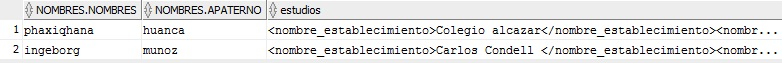
\includegraphics [scale=0.73]{capitulo3/images/xmlresultado1.jpg} \end{center}
 \caption{\label{resultado1}Resultado de consulta a columna XMLTYPE (con tags)}
 \end{figure}
%%%%%%%%%%%%%%%%%%%%%%%%%%%%%%%%%%%%%%%%%%%%%%%%%%%%%%%%%%%%%%%%%%

\noindent Por otro lado, en el c�digo \ref{ejemxml4} se presenta la consulta en
caso de que se desee listar cada lugar (como tupla) donde estudi� la persona. Se puede
observar su resultado en la figura \ref{resultado2}. En el caso de que se quiera
listar todos los nombres de establecimientos sin repetirlos, se debe incluir el
comando \tn{DISTINCT}.
\\

\begin{lstlisting}[language=SQL, caption={Columna XMLType en caso de estudio},
 label=ejemxml4] 
select extractValue(x.column_value, 'estudio/nombre_establecimiento') as nombre_establecimiento
from personalxml p,
table(XMLSequence(extract(p.curriculum,'curriculum/estudios/estudio'))) x;
\end{lstlisting}

 %%%%%%%%%%%%%%%%%%%%%%%%%%%%%%%%%%%%%%%%%%%%%%%%%%%%%%%%%%%%%%%%%%%%%
 \begin{figure}[H]
 \begin{center}
  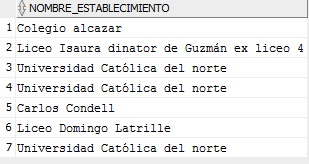
\includegraphics [scale=0.7]{capitulo3/images/xmlresultado2.jpg} \end{center}
 \caption[Resultado a columna XMLTYPE nodos]{\label{resultado2}Resultado de
 consulta a columna XMLTYPE (Tupla por cada nodo)}
 \end{figure}
%%%%%%%%%%%%%%%%%%%%%%%%%%%%%%%%%%%%%%%%%%%%%%%%%%%%%%%%%%%%%%%%%%

\noindent Para actualizar datos dentro de una columna XMLTYPE se debe tener
claro conocimiento de qu�  se desea actualizar exactamente, el
documento completo o s�lo algunos nodos seg�n alguna restricci�n. Por ejemplo en c�digo \ref{ejemxml5} se
actualiza la columna XMLTYPE con un documento nuevo. \\


\begin{lstlisting}[language=SQL, caption={Actualizaci�n de Columna XMLType en
caso de estudio}, label=ejemxml5] 
UPDATE personalxml p SET p.curriculum = XMLTYPE('<curriculum><estudios>
<estudio nivel="Ense�anza Superior">
			<nombre_establecimiento>Universidad Cat�lica del norte</nombre_establecimiento>
			<carrera>Ingenier�a Civil Plan Com�n</carrera>
			<ciudad>Antofagasta</ciudad>
		</estudio>
		<estudio nivel="Ense�anza Superior">
			<nombre_establecimiento>Universidad Cat�lica del norte</nombre_establecimiento>
			<carrera>Ingenier�a de Ejecuci�n en Computaci�n e Inform�tica</carrera>
			<ciudad>Antofagasta</ciudad><fecha_egreso>2011</fecha_egreso>
		</estudio>
	</estudios>
	<cursos>
		<curso area="Inform�tica"><tipo>Diplomado</tipo>
			<nombre>Redes de datos</nombre><horas>50</horas>
		</curso>
		<curso area="Inform�tica"><tipo>Capacitaci�n</tipo>
			<nombre>6to WORKSHOP Iniciativa CLGRID UCN</nombre>
			<horas>30</horas></curso>	
		<curso area="Inform�tica"><tipo>Capacitaci�n</tipo>
			<nombre>Tutorial on Distributed High Performance Computing</nombre>
			<horas>10</horas></curso>
	</cursos>
	<idiomas>
		<idioma nombre="Espa�ol"><nivel>Nativo</nivel></idioma>
		<idioma nombre="Ingles"><nivel>Medio</nivel></idioma>
	</idiomas>
</curriculum>') WHERE p.rut.num_correlativo=12345678;
\end{lstlisting}

\noindent Los cambios realizados pueden ser comprobados en la figura
\ref{resultado3}

%%%%%%%%%%%%%%%%%%%%%%%%%%%%%%%%%%%%%%%%%%%%%%%%%%%%%%%%%%%%%%%%%%%%%
 \begin{figure}[H]
 \begin{center}
  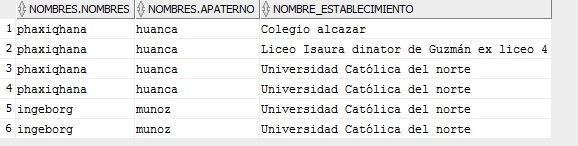
\includegraphics [scale=1]{capitulo3/images/xmlresultado3.jpg} \end{center}
 \caption[Resultado a columna XMLTYPE despu�s
 UPDATE]{\label{resultado3}Resultado de consulta a columna XMLTYPE despu�s de un UPDATE}
 \end{figure}
%%%%%%%%%%%%%%%%%%%%%%%%%%%%%%%%%%%%%%%%%%%%%%%%%%%%%%%%%%%%%%%%%%

\noindent Si se desea actualizar un nodo en particular dentro del documento XML,
es necesario tener alg�n identificador. Seg�n el esquema del documento del
caso de estudio no se consider� ning�n tipo de identificador, pero es
posible filtrar por alg�n elemento. En el ejemplo del c�digo \ref{ejemxml6} se
realiza la actualizaci�n de los nodos idioma, en la figura \ref{resultado4} se muestra el resultado de la consulta antes de la
actualizaci�n y en la figura \ref{resultado5} despu�s de la actualizaci�n.

%%%%%%%%%%%%%%%%%%%%%%%%%%%%%%%%%%%%%%%%%%%%%%%%%%%%%%%%%%%%%%%%%%%%%
 \begin{figure}[H]
 \begin{center}
  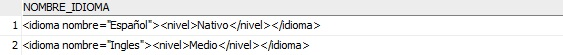
\includegraphics [scale=1]{capitulo3/images/xmlresultado4.jpg} \end{center}
 \caption[Resultado a columna XMLTYPE antes UPDATE nodos]{\label{resultado4}Resultado de consulta a columna XMLTYPE antes de
 UPDATE de nodos}
 \end{figure}
%%%%%%%%%%%%%%%%%%%%%%%%%%%%%%%%%%%%%%%%%%%%%%%%%%%%%%%%%%%%%%%%%%

\begin{lstlisting}[language=SQL, caption={Actualizaci�n nodos de Columna XMLType
en caso de estudio}, label=ejemxml6] 
UPDATE personalxml p SET curriculum = updateXML 
(curriculum, '/curriculum/idiomas/idioma/nivel/text()','Avanzado')
where existsNode(curriculum,'/curriculum/idiomas/idioma')=1 
and p.rut.num_correlativo=12345678;
\end{lstlisting}

%%%%%%%%%%%%%%%%%%%%%%%%%%%%%%%%%%%%%%%%%%%%%%%%%%%%%%%%%%%%%%%%%%%%%
 \begin{figure}[H]
 \begin{center}
  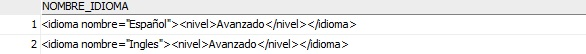
\includegraphics [scale=1]{capitulo3/images/xmlresultado5.jpg} \end{center}
 \caption[Resultado a columna XMLTYPE despu�s UPDATE nodos]{\label{resultado5}Resultado de consulta a columna XMLTYPE despu�s de un UPDATE de nodos}
 \end{figure}
%%%%%%%%%%%%%%%%%%%%%%%%%%%%%%%%%%%%%%%%%%%%%%%%%%%%%%%%%%%%%%%%%%

\noindent Finalmente la eliminaci�n de contenido de una columna XMLType, se
trata igual que la eliminaci�n de otro tipo de datos. Por ejemplo, en el c�digo
\ref{ejemxml7} se eliminan todos las filas de idioma que sean del nivel
``Medio'', en la figura \ref{resultado4} se muestra el resultado de la consulta antes de la
eliminaci�n y en la figura \ref{resultado6} despu�s de la misma. \\


%%%%%%%%%%%%%%%%%%%%%%%%%%%%%%%%%%%%%%%%%%%%%%%%%%%%%%%%%%%%%%%%%%

\begin{lstlisting}[language=SQL, caption={Actualizaci�n nodos de Columna XMLType
en caso de estudio}, label=ejemxml7] 
UPDATE personalxml p set 
p.curriculum=deletexml(p.curriculum,'/curriculum/idiomas/idioma[nivel="Medio"]')
where p.rut.num_correlativo=12345678;
\end{lstlisting}

%%%%%%%%%%%%%%%%%%%%%%%%%%%%%%%%%%%%%%%%%%%%%%%%%%%%%%%%%%%%%%%%%%%%%
 \begin{figure}[H]
 \begin{center}
  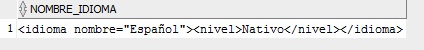
\includegraphics [scale=1]{capitulo3/images/xmlresultado6.jpg} \end{center}
 \caption[Resultado a columna XMLTYPE despu�s DELETE
 nodos]{\label{resultado6}Resultado de consulta a columna XMLTYPE despu�s de un DELETE de nodos}
 \end{figure}
%%%%%%%%%%%%%%%%%%%%%%%%%%%%%%%%%%%%%%%%%%%%%%%%%%%%%%%%%%%%%%%%%%

\section{Comparaci�n de resultados} \label{comparacion_resultados}

\noindent Los criterios a evaluar en cada implementaci�n, son los siguientes:

\begin{itemize}
  \item Facilidad de modelamiento
  \item Complejidad de aprendizaje por parte del desarrollador y/o DBA
\end{itemize}



\par \noindent El modelamiento de los datos es claramente m�s sencillo en el
modelo objeto relacional, ya que se utilizan las cualidades de la orientaci�n al
objeto, lo que permite al desarrollador codificar su aplicaci�n sin preocuparse
de las inserciones fragmentadas y redundancia de los datos (en el caso de
atributos multivaluados en relacionamientos N a N). La creaci�n de objetos
complejos dentro del SQL, facilita enormemente el modelamiento, ya que existe
mayor sem�ntica y cada tipo de objeto es consistente con el mundo real, a la
vez reemplazar los atributos derivados con m�todos que calculen los datos
necesarios, como por ejemplo la edad de una persona
o la cantidad de ventas realizadas por un vendedor, entre otros.
Por otro lado, al permitir capacidades tan b�sicas como los subtipos, posibilita
la implementaci�n de herencia de tipos, que al igual que en la orientaci�n al
objeto, se heredan los atributos y m�todos.\\

\noindent Si se desea tener un listado de datos dentro de un objeto, estos se
almacenan en un arreglo, sin la necesidad de generar una tabla exclusiva para almacenar
dichos datos, adem�s esta informaci�n puede ser desplegada con facilidad a
trav�s de una consulta, dejando atr�s los joins y registros duplicados. En el
c�digo \ref{codigoselectarray} se presenta una consulta sencilla del caso de
estudio en donde se despliegan todos los celulares de un No
Docente (en donde los celulares son un varray del tipo celular\_persona\_ob),
el resultado de dicha consulta se encuentra en la figura \ref{resultadoarray}. \\

%%%%%%%%%%%%%%%%%%%%%%%%%%%%%%%%%%%%%%%%%%%%%%%%%%%%%%%%%%%%%%%%%

\begin{lstlisting}[language=SQL, caption={Ejemplo de consulta a listado de
celulares de un No Docente}, label=codigoselectarray] 
SELECT C.* FROM NO_DOCENTE P, TABLE (P.NUM_CELULARES) C 
WHERE P.RUT.NUM_CORRELATIVO=1234567;
\end{lstlisting}

%%%%%%%%%%%%%%%%%%%%%%%%%%%%%%%%%%%%%%%%%%%%%%%%%%%%%%%%%%%%%%%%%%%%%

%%%%%%%%%%%%%%%%%%%%
\begin{figure}[H]
 \begin{center}
  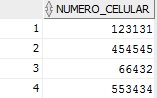
\includegraphics [scale=1.1]{capitulo3/images/resultadoarray.jpg}
  \end{center}
 \caption[Resultado de consulta a listado de
 celulares]{\label{resultadoarray}Resultado de consulta a listado de celulares
 de un No Docente}
 \end{figure}
%%%%%%%%%%%%%%%%%%

\par \noindent La gran diferencia recae en la
sintaxis de cada implementaci�n, esto es debido a la naturaleza de ambos modelos, es decir, para una consulta en el modelo relacional
se hace necesario realizar el join de tablas expl�citamente en las cl�usulas
FROM y WHERE de la sentencia; sin embargo, cuando se aprovecha la utilizaci�n de punteros en el modelo objeto
relacional, es posible ``navegar'' hacia las dem�s tablas involucradas en la
consulta, por lo que no es necesario especificar todas las tablas en la cl�usula FROM de la sentencia, sino que basta solamente con utilizar la tabla a consultar 
en la cl�usula FROM de la sentencia. 

\noindent Para ejemplificar lo antes descrito, se
presenta una consulta que se encarga de desplegar el nombre del tipo de programa, su abreviatura, nombre de la
asignatura y nombre de nivel de ense�anza de dicha asignatura, de cada detalle
de programa existente en la base de datos.
\noindent  En los c�digos \ref{casoR} y
\ref{casoOR} se puede visualizar la consulta realizada en el modelo relacional y en el modelo objeto relacional respectivamente. \\

%%%%%%%%%%%%%%%%%%%%%%%%%%%%%%%%%%%%%%%%%%%%%%%%%%%%%%%%%%%%%%%%%

\begin{lstlisting}[language=SQL, caption={Ejemplo consulta modelo relacional
en caso de estudio}, label=casoR] 
SELECT PT.NOM_PT, PT.ABREV, A.NOM_ASIG, N.NOM_NIVEL
FROM PROGRAMA_TIPO PT, ASIGNATURA A, NIVEL N, 
	 			DETALLE_PROGRAMA DP
WHERE PT.ID_PT=DP.ID_PT AND DP.ID_ASIG=A.ID_ASIG 
AND		A.ID_NIVEL=N.ID_NIVEL;
\end{lstlisting}

%%%%%%%%%%%%%%%%%%%%%%%%%%%%%%%%%%%%%%%%%%%%%%%%%%%%%%%%%%%%%%%%%%%%%

%%%%%%%%%%%%%%%%%%%%%%%%%%%%%%%%%%%%%%%%%%%%%%%%%%%%%%%%%%%%%%%%%

\begin{lstlisting}[language=SQL, caption={Ejemplo consulta modelo
objeto relacional en caso de estudio}, label=casoOR] 
SELECT DP.PROGRAMA_TIPO.NOM_PT, DP.PROGRAMA_TIPO.ABREV, DP.ASIGNATURA.NOM_ASIG,
	   DP.ASIGNATURA.CURSO_DICTA.REFNIVEL.NOM_NIVEL
FROM DETALLE_PROGRAMA DP;
\end{lstlisting}

%%%%%%%%%%%%%%%%%%%%%%%%%%%%%%%%%%%%%%%%%%%%%%%%%%%%%%%%%%%%%%%%%%%%%

\noindent Se propone utilizar notaci�n UML para el modelo objeto relacional, ya
que trabaja directamente con objetos, atributos y sus respectivos m�todos. Se
sugiere utilizar el algoritmo de transformaci�n de modelo relacional a objeto
relacional detallado en la secci�n \ref{algoritmoor} del presente cap�tulo,
puesto que el resultado final ser� acorde al modelo realizado en UML.
Adem�s seg�n las pruebas realizadas, esta es la transformaci�n adecuada si se
desea desarrollar una aplicaci�n que posea navegabilidad bidireccional. 

\noindent Se requiere de un tiempo y dedicaci�n por parte del desarrollador para
obtener un nivel de aprendizaje adecuado, ya que puede resultar confuso y
complejo en un principio, puesto que existen diferencias con el SQL tradicional
el cual utiliza el modelo relacional. Pero si se tiene una base en la
orientaci�n al objeto, no deber�a requerir de tanto tiempo de capacitaci�n y
s�lo ser�a necesario estudiar los conceptos y la nueva sintaxis que viene de la
mano del modelo objeto relacional.


\noindent Por otro lado, el modelo relacional permite un modelado sencillo con
consultas potentes. Si no se posee conocimientos en bases de datos relacionales, el tiempo de
aprendizaje por parte del desarrollador es claramente inferior al del
objeto relacional.
En cambio s� se est� familiarizado con este modelo resulta sumamente f�cil
implementar cualquier problema medianamente complejo del mundo real. Por el contrario, si el problema
es muy grande la cantidad de tablas y relacionamientos aumentan, esto provoca que las consultas sean m�s complejas de escribir, incluso pueden llegar a ser 
confusas cuando se requiere de muchos joins (por ejemplo entre m�s de 10 tablas). 

\noindent Otro gran inconveniente es la creaci�n de tablas innecesarias, 
como se mencion� anteriormente un atributo multivaluado en el modelo relacional, autom�ticamente genera una tabla,
produciendo una redundancia de datos en dicha tabla, cuando solamente deber�a
bastar con guarda un listado dentro de la misma tabla, por ejemplo el listado notas de un
alumno en una asignatura en particular. 

\noindent Adem�s cabe destacar la cantidad de tablas que se generan en la
implementaci�n del caso de estudio en cada modelo, claramente en el modelo
objeto relacional se disminuye la cantidad de tablas dr�sticamente, ya que se
eliminan todas las tablas generadas por los atributos multivaluados y los relacionamientos N a N. En las figuras \ref{count1} y \ref{count2} se visualiza la cantidad de tablas del modelo relacional y el modelo objeto relacional respectivamente.
\\
%%%%%%%%%%%%%%%%%%%%
\begin{figure}[H]
 \begin{center}
  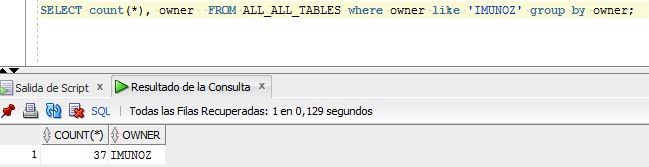
\includegraphics [scale=0.9]{capitulo3/images/count1.jpg}
  \end{center}
 \caption[Cantidad tablas modelo relacional]{\label{count1}Cantidad tablas modelo relacional}
 \end{figure}
%%%%%%%%%%%%%%%%%%
\newpage
%%%%%%%%%%%%%%%%%%%
\begin{figure}[H]
 \begin{center}
  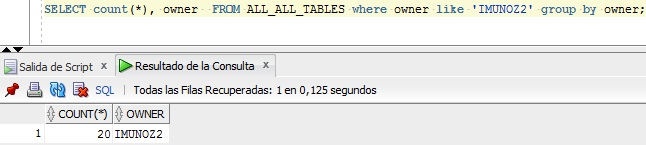
\includegraphics [scale=0.9]{capitulo3/images/count2.jpg}
  \end{center}
 \caption[Cantidad tablas modelo objeto relacional]{\label{count2}Cantidad tablas modelo objeto relacional}
 \end{figure}
%%%%%%%%%%%%%%%%%%


\noindent La implementaci�n de columnas del tipo XML en una base de datos objeto
relacional, es relativamente sencilla, s�lo requiere de la creaci�n del esquema
del documento XML y validar con dicho esquema cada tupla que se desea
insertar, con el prop�sito de verificar que los datos insertados efectivamente
cumplen las restricciones detalladas en el esquema.
En cuanto a manejo de datos s�lo se debe tener claro c�mo funciona XPath y
obtener cierto nivel de expertiz en su funcionamiento, puesto que las funciones
de extracci�n de datos en XML son distintas a las que se manejan en el SQL
tradicional.
Luego resulta simple la ejecuci�n de consultas ya sea de selecci�n, actualizaci�n o eliminaci�n. Existen algunas funciones caracter�sticas de XML
que facilitan bastante dicha labor, por lo que el tiempo de aprendizaje por parte del desarrollado es m�nimo.

\noindent Aunque en este trabajo de titulaci�n no se desarrollaron experiencias
para ver tiempos de respuestas en el desempe�o de las consultas, existen
diversas investigaciones que indican significativas mejoras en los tiempos de
respuestas, esto se ve corroborado por experiencias que se han realizado
en \cite{comparacion} y \cite{bucky}.
En el anexo \ref{anexo4} se presenta una parte de los resultados.


\noindent En la figura \ref{tablaresumen} se presenta un resumen con el
comportamiento de los criterios de cada modelo. 
%%%%%%%%%%%%%%%%%%%%
\begin{figure}[H]
 \begin{center}
  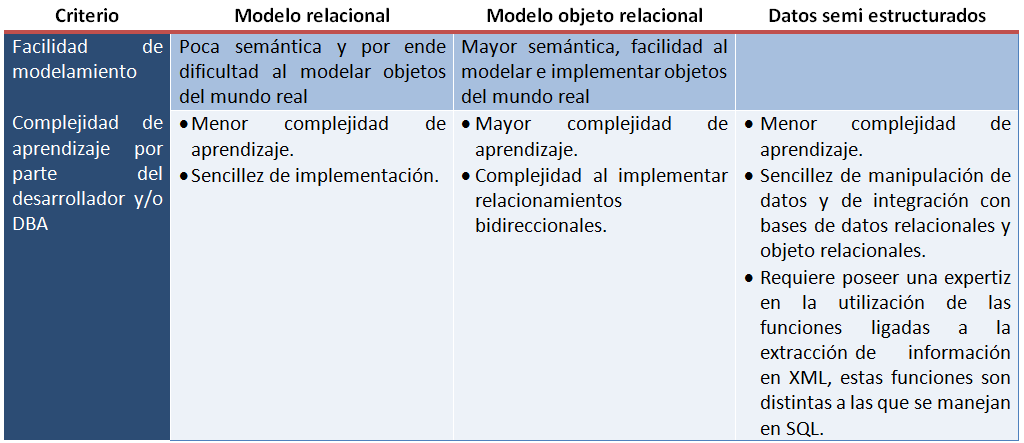
\includegraphics [width=5.7in,height=2.5in]{capitulo3/images/tablaresumen.png}
  \end{center}
 \caption[Tabla resumen de criterios]{\label{tablaresumen}Tabla resumen de
 criterios}
 \end{figure}
%%%%%%%%%%%%%%%%

\noindent En el desarrollo del caso de estudio, se resume las caracter�sticas
del modelo relacional, modelo objeto relacional y datos semi estructurados,
mostrados en las tablas \ref{tablamodelorelacional}, \ref{tablamodeloor} y
\ref{modeloxml} respectivamente.

\begin{table}[H]
    \begin{tabular}{|p{7cm}|p{7cm}|}
    \hline
    \multicolumn{2}{|c|}{\tn{Modelo Relacional}} \\ \hline
    \tn{Ventajas }                     & \tn{Desventajas}                                
    \\ \hline Lenguaje de consultas potente & No soporta la navegabilidad, se debe acceder a los relacionamientos a trav�s de Joins \\ \hline
    Simple y puro                 & Poca sem�ntica                                                                        \\ \hline
    F�cil de aprender                            & Fragmentaci�n de datos y  redundancia \\ \hline 
    Muy r�pido de implementar                            & Dificultad al modelar objetos del mundo real \\ \hline 
    Sencillez al implementar relacionamientos          & Tipo de datos
    sencillos, no permite objetos complejos \\ \hline
    \end{tabular}
    \caption {\label{tablamodelorelacional} Ventajas y desventajas del modelo
    relacional}
\end{table}

\begin{table}[H]
    \begin{tabular}{|p{7cm}|p{7cm}|}
    \hline
    \multicolumn{2}{|c|}{\tn{Modelo Objeto Relacional}} \\ \hline
    \tn{Ventajas }                     & \tn{Desventajas}                                
    \\ \hline Sem�ntica en el modelado & Mayor complejidad de aprendizaje
     \\ \hline Existe navegabilidad & Mayores costos (en tiempos de
     implementaci�n) 
     \\ \hline Eliminaci�n de Joins                             &  Complicado al
     momento implementar relacionamientos bidireccionales \\ \hline Soporte de
     objetos complejos y herencia & Para implementar relacionamiento
     bidireccionales cuando los objetos poseen muchos relacionamientos con
     otros objetos, se debe generar un tipo y tabla intermediario, ya que los
     varray y nested tables no permiten su implementaci�n correctamente
     \\
     \hline Reutilizaci�n y compartici�n & ~ \\ \hline Mejora significativamente la productividad (las consultas son
       m�s legibles) & ~ 
       \\ \hline Preserva el cuerpo de conocimiento y
       experiencia alcanzado con las bases de datos relacionales & ~
        \\ \hline El tama�o de las consultas disminuye al momento de consultar
        relacionamientos, gracias a las referencias y eliminaci�n de joins & ~
       
       \\ \hline
    \end{tabular}
    \caption {\label{tablamodeloor}Ventajas y desventajas del modelo
    objeto relacional}
\end{table}

\begin{table}[H]
    \begin{tabular}{|p{7cm}|p{7cm}|}
    \hline
    \multicolumn{2}{|c|}{\tn{Datos semi estructurados}} \\ \hline
    \tn{Ventajas }                     & \tn{Desventajas}                                
    \\ \hline Intercambio flexible de datos relacionales utilizando XML & 
    Requiere comprender c�mo describir la estructura y restricciones del
    documento xml para lograr crear esquemas XML correctamente.
    \\
    \hline Publicar datos relacionales como XML                &  Requiere
    poseer una expertiz en la utilizaci�n de las funciones ligadas a la
    extracci�n de informaci�n en XML, estas funciones son distintas a las que se
    manejan en SQL \\ \hline Descomponer XML en datos relacionales                          
    &                                                   \\ \hline Fiabilidad en la gesti�n de datos XML                            &                                           \\ \hline Manipulaci�n, b�squeda, almacenamiento                             &                                                                \\ \hline Integraci�n con datos relacionales                            & ~                                                                                     \\ \hline
    Permite almacenar datos XML de forma nativa 
en la base de datos                             & ~                                        
\\ \hline F�cil de aprender                           & ~                                                                                     
\\ \hline Provee una gran flexibilidad en cuanto a la 
estructura sin deteriorar el desempe�o  &\\ \hline

    \end{tabular}
    \caption {\label{modeloxml}Ventajas y desventajas de XML/SQL}
\end{table}
 %\chapter{AN�LISIS E INTERPRETACI�N DE RESULTADOS} \label{capitulo4}

\section{An�lisis de los resultados}

\noindent En este cap�tulo se presentan los resultados de la investigaci�n
realizada, el cual comprende el an�lisis e interpretaci�n de resultados
y recomendaciones.

\subsection{Criterios de comparaci�n}

\noindent Los criterios a evaluar en cada implementaci�n, son los siguientes:

\begin{itemize}
  \item Facilidad de modelamiento
  \item Complejidad de aprendizaje por parte del desarrollador y/o DBA
\end{itemize}

% \noindent Cabe destacar que el desempe�o de consultas ser�
% comparado con informaci�n adquirida de otras investigaciones, ya que para obtener resultados fidedignos es 
% irrelevante el origen de los datos. Se quiso aprovechar el trabajo ya
% realizado en dichas investigaciones y as� concentrar el esfuerzo en la
% implementaci�n.



\subsection{Comparaci�n de resultados} \label{comparacion_resultados}







\section{Recomendaciones}

\noindent Si se desea crear un sistema desde cero, considerando que el
desarrollo ser� bajo el paradigma orientaci�n al objeto, es muy recomendable
implementar la base de datos en el modelo objeto relacional. Es posible que esto
tome mayor tiempo de implementaci�n, ya que el desarrollador primero deber�
interiorizarse con el modelo, c�mo se crean los tipos de objetos, los
relacionamientos, referencias, tablas de objetos, entre otros. Pero obtendr�
una sintaxis m�s limpia al momento de realizar las consultas a la base de datos.
Y por consecuencia, al momento de realizar mantenimiento de dicha aplicaci�n,
resultar� sumamente sencillo de llevar a cabo porque existe una gran base de
conocimiento en dicho paradigma.

\noindent Por otro lado, si se desea migrar un sistema actual que se encuentra
complemente implementado en el modelo relacional, es probable que sea muy
complicado, puesto que habr�a que realizar una transformaci�n tanto del
c�digo desarrollado como de la base de datos. Es
posible que tome un tiempo elevado, pero con buenos resultados, ya que luego de la migraci�n el c�digo del sistema
deber�a ser m�s sencillo de mantener gracias a la sem�ntica del modelo
implementado.

\noindent Si se desea crear aplicaciones web donde no existan muchas inserciones
y principalmente la base de datos ser� utilizada para la lectura de datos como
por ejemplo un blog o una wiki, se propone implementar mediante datos semi
estructurados XML, ya que es f�cil de mantener y usar.
S�lo se debe tener un cierto conocimiento en la extracci�n de datos XML.
El desarrollo y puesta en marcha tomar�a menos tiempo.

\noindent En el caso de que se desee crear aplicaciones o sistemas que no est�n
bajo el paradigma orientaci�n al objeto, no tendr�a mucho sentido utilizar el
modelo objeto relacional, ya que el desarrollo ser�a m�s estructural y bastar�a
con utilizar el modelo relacional que para ese tipo de sistema resulta ser el
m�s apropiado.

\noindent Si es una aplicaci�n transaccional peque�a, como control de bodega o
carrito de compras, lo m�s sencillo ser�a utilizar el modelo relacional, ya que
generalmente ese tipo de aplicaciones son f�ciles de modelar debido a su baja
complejidad, por lo que resultar�a innecesaria la creaci�n de objetos complejos.

\noindent En el caso de aplicaciones m�viles sencillas, como por ejemplo:
Lista de compras, notas personales, video juegos con puntajes locales, entre
otros, en donde los datos son almacenados en el mismo dispositivo, se recomienda
utilizar XML, pues no es necesario disponer de una base de datos para almacenar 
informaci�n que s�lo se visualizar� en dicho dispositivo. 

\noindent Para problemas muy complejos, con una gran cantidad tablas y/o
relacionamientos y que deban ser implementados con urgencia en un tiempo muy
corto, se recomienda emplear una base de datos relacional, puesto que su creaci�n es mucho
m�s r�pida que la objeto relacional y no requiere aprendizaje
extra.

\noindent Para cualquier tipo de aplicaci�n en donde se requiera de muchas
consultas donde exista una gran cantidad de agrupamientos con un inmenso
n�mero de datos, es recomendable el uso del modelo objeto relacional, seg�n
los datos obtenidos en \ref{comparacion_resultados} este modelo es mucho
m�s eficiente que el relacional y sencillo de escribir, ya que se utilizan
punteros y no existen joins.

  \chapter{CONCLUSIONES}

\noindent En este cap�tulo se exponen las conclusiones de este trabajo de
titulaci�n.
Para ello, primero se menciona una serie de recomendaciones donde se detalla
qu� tipo de base de datos utilizar seg�n la aplicaci�n a desarrollar, luego se
analiza el cumplimiento de los objetivos mencionados en el cap�tulo
\ref{capitulo1} y se describen las propuestas que se pueden llevar a cabo en el futuro a partir del trabajo
desarrollado en este trabajo de titulaci�n.

\section{Recomendaciones en la elecci�n del tipo de base de datos para una
aplicaci�n particular}\label{recomendacion}

\noindent Si se desea crear un sistema desde cero, considerando que el
desarrollo ser� bajo el paradigma de la orientaci�n al objeto, es muy
recomendable implementar la base de datos en el modelo objeto relacional. Es posible que esto
tome mayor tiempo de implementaci�n, ya que el desarrollador primero deber�
interiorizarse con el modelo, c�mo se crean los tipos de objetos, los
relacionamientos, referencias, tablas de objetos, entre otros. Pero obtendr�
una sintaxis m�s limpia al momento de realizar las consultas a la base de datos.
Y por consecuencia, al momento de realizar mantenimiento de dicha aplicaci�n,
resultar� sumamente sencillo de llevar a cabo porque existe una gran base de
conocimiento en dicho paradigma.

\noindent Por otro lado, si se desea migrar un sistema actual que se encuentra
complemente implementado en el modelo relacional, es probable que sea muy
complicado, puesto que habr�a que realizar una transformaci�n tanto del
c�digo desarrollado como de la base de datos. Es
posible que tome un tiempo elevado, pero con buenos resultados, ya que luego de la migraci�n el c�digo del sistema
deber�a ser m�s sencillo de mantener gracias a la sem�ntica del modelo
implementado.

\noindent Si se desea crear aplicaciones web donde existe una comunicaci�n con
otras aplicaciones c�dificadas en otros lenguajes de programaci�n, se
propone implementar con datos semi estructurados XML para comunicar el lenguaje
de la aplicaci�n web con las otras aplicaciones. Resulta provechoso almacenar
los datos en XML, ya que es f�cil de mantener y utilizar. S�lo se debe tener un cierto conocimiento en la extracci�n de datos XML; el
desarrollo y puesta en marcha tomar�a menos tiempo.

%no existan muchas inserciones y principalmente la base de datos ser�
%utilizada para la lectura de datos como por ejemplo un blog o una wiki, se
% propone implementar mediante datos semi estructurados XML, ya que es f�cil de mantener y usar.


\noindent En el caso de que se desee crear aplicaciones o sistemas que no est�n
bajo el paradigma orientaci�n al objeto, no tendr�a mucho sentido utilizar el
modelo objeto relacional, ya que el desarrollo ser�a m�s estructural y bastar�a
con utilizar el modelo relacional que para ese tipo de sistema resulta ser el
m�s apropiado.

\noindent Si es una aplicaci�n transaccional peque�a, como control de bodega o
carrito de compras, lo m�s sencillo ser�a utilizar el modelo relacional, ya que
generalmente ese tipo de aplicaciones son f�ciles de modelar debido a su
similitud con los objetos del mundo real, por lo que resultar�a innecesaria la
creaci�n de objetos complejos.

% \noindent En el caso de aplicaciones m�viles sencillas, como por ejemplo:
% Lista de compras, notas personales, video juegos con puntajes locales, entre
% otros, en donde los datos son almacenados en el mismo dispositivo, se recomienda
% utilizar XML, pues no es necesario disponer de una base de datos para almacenar 
% informaci�n que s�lo se visualizar� en dicho dispositivo. 

\noindent Para problemas muy complejos, con una gran cantidad tablas y/o
relacionamientos y que deban ser implementados con urgencia en un tiempo muy
corto, se recomienda emplear una base de datos relacional, puesto que su creaci�n es mucho
m�s r�pida que la objeto relacional y no requiere aprendizaje
extra.

\noindent Para cualquier tipo de aplicaci�n en donde se requiera de muchas
consultas donde exista una gran cantidad de agrupamientos con un inmenso
n�mero de datos, es recomendable el uso del modelo objeto relacional, seg�n
los datos obtenidos en el anexo \ref{anexo4} y la secci�n 
\ref{comparacion_resultados} este modelo es mucho m�s eficiente que el relacional y sencillo de escribir, ya que se utilizan
punteros y no existen joins.


\section{Cumplimiento de los objetivos}

\noindent Al comienzo de este trabajo de titulaci�n, se propusieron una serie de
objetivos espec�ficos que eran necesarios para alcanzar el objetivo
general: ``Evaluar y comparar la implementaci�n de una base de datos relacional
con respecto a una base de datos objeto relacional y datos semi estructurados
en el sistema de administraci�n de base de datos Oracle, utilizando las
funciones disponibles en el servidor del SABD, con el fin de generar una gu�a que en base a
criterios claros permita determinar cu�l es el tipo de base de datos m�s
adecuada a utilizar bajo ciertas caracter�sticas''.

\noindent A continuaci�n, se analizar�n en qu� medida se ha conseguido alcanzar
cada uno de ellos:

\begin{itemize}
  \item \tn{Objetivo 1}: Estudiar, seleccionar y utilizar funciones del sistema
  de administraci�n de base de datos relacional Oracle 11G, que permitan la implementaci�n de bases
de datos objeto relacional y XML.

%\begin{itemize}
\noindent Para satisfacer este objetivo, se ha llevado a cabo una labor de
investigaci�n y documentaci�n sobre el SABD Oracle y c�mo se implementan los objetos, m�todos y
columnas del tipo XML dentro de una base de datos objeto relacional.
%\end{itemize}

\item \tn{Objetivo 2}: Comprender los m�ltiples m�todos de implementaci�n de los
modelos mencionados con anterioridad para ser capaz de seleccionar adecuadamente entre
ellos seg�n la aplicaci�n a desarrollar.

% \begin{itemize}

\noindent Sin duda esta tarea fue la m�s compleja, ya que las restricciones del
motor hicieron que la implementaci�n del modelo objeto relacional no fuera como se
planteaba en la teor�a. Sin embargo, en la secci�n \ref{recomendacion} del
presente cap�tulo se recomienda qu� tipo de aplicaciones se deben o pueden
desarrollar seg�n cada modelo. 
% \end{itemize}

\item \tn{Objetivo 3}: Dise�ar el caso de estudio para luego implementarlo con
Oracle 11G en una base de datos relacional, objeto relacional y datos semi
estructurados como XML.

\begin{itemize}

\item El caso de estudio fue un problema en el que la memorista se vi�
enfrentada en la vida real y quiso ver las m�ltiples ganancias de implementarlo
en el modelo objeto relacional o utilizar datos semi estructurados. Pero, este result� ser muy
grande y complejo lo que repercuti� en toda la fase de implementaci�n, su gran
cantidad de relacionamientos N a N, sirvi� para detectar algunas falencias que
existen en Oracle para implementar navegabilidad bidireccional en objetos con
muchos relacionamientos N a N.

\item Claramente al tener mayor familiaridad con el modelo relacional, se
 hace muy simple implementar el caso de estudio seg�n el algoritmo de
 transformaci�n de entidad relacionamiento a relacional \cite{navathe}, sin duda
 es un modelo muy probado y confiable, pero a la vez se queda corto en muchas
 funcionalidades que el objeto relacional si soluciona, la redundancia de datos
 y la creaci�n de tablas innecesarias que fragmenta a�n m�s la informaci�n, le
 resta puntos al momento de elegir un modelo.
 
 \item De la teor�a a la implementaci�n del modelo objeto relacional existieron
 muchos obst�culos y dificultades, como por ejemplo la utilizaci�n de tablas
 anidadas, en la teor�a esa era la opci�n correcta y m�s viable para los relacionamientos de 1 a N y N a N,
 sin embargo, para el caso de estudio que era altamente complejo fue imposible
 lograr utilizar dicha estructura de datos y mantener la navegabilidad bidireccional, ya que si la referencia
 de un objeto es almacenada en una tabla anidada y su estructura cambia luego de ser almacenada, la tabla
 anidada quedar� en un estado inv�lido. En cambio, si la base de datos es
 implementada con navegabilidad unidireccional tal como se presenta en
 \cite{susan}, se puede llevar a cabo sin inconvenientes.
 
 \item La mejor soluci�n para dicho problema fue utilizar un varray para los
 relacionamientos, considerando un tama�o m�ximo razonable e implementando un
 m�todo dentro del objeto, que verifique en cada inserci�n que el varray no ha
 llegado al tope.
 Esta soluci�n es mucho m�s sencilla de implementar y f�cil de entender, ya que su
 sintaxis es m�s limpia y menos compleja que una tabla anidada. Sin embargo, se
 present� el mismo problema descrito con anterioridad al momento de mantener la
 navegabilidad bidireccional en relacionamientos de N a N. Para solucionar este
 inconveniente se cre� un nuevo tipo intersecci�n, el cual posee una referencia
 a cada objeto con el que se tiene un relacionamiento, para luego crear un
 listado (varray) de referencias a ese nuevo objeto intersecci�n y es dicho
 listado el que se agrega a cada objeto del relacionamiento.
  
\item No existieron mayores inconvenientes al implementar columnas del tipo XML,
aunque se requiere poseer una expertiz en la utilizaci�n de las funciones
ligadas a la extracci�n de informaci�n en XML, ya que estas funciones son
distintas a las que se manejan en SQL tradicional.

 \end{itemize}

\item \tn{Objetivo 4}: Definir criterios de comparaci�n para las
implementaciones tales como:
Desempe�o en consultas, facilidad de modelamiento, complejidad de aprendizaje
por parte del desarrollador y/o DBA, entre otros.

% \begin{itemize}
\noindent En la secci�n \ref{comparacion_resultados} fueron presentados los criterios de
comparaci�n que se utilizaron para realizar el an�lisis de resultados. 
% \end{itemize}

\item \tn{Objetivo 5}: Realizar un an�lisis de resultados, en donde se compare
cada una de las implementaciones, con el fin de
estructurar una gu�a con los beneficios y desventajas dependiendo de la
aplicaci�n a desarrollar, seg�n los criterios de comparaci�n.

\begin{itemize}
\item Al igual que el item anterior en la secci�n \ref{comparacion_resultados} fueron
presentados el an�lisis e interpretaci�n de los resultados obtenidos seg�n los criterios de
comparaci�n. 

% \item El desempe�o en casi todas las consultas fue altamente superior en el
% modelo relacional, existen excepciones como en agrupamientos sencillos con
% muchos datos y utilizando having en donde el modelo objeto relacional es mucho
% m�s eficiente que el relacional.

 \item Se ha podido establecer que las bases de datos objeto relacional 
son m�s sencillas de modelar, lo cual queda demostrado
en la versi�n UML del caso de estudio.
Una vez que se entiende el funcionamiento y sintaxis resulta muy f�cil de
utilizar. Sin embargo el aprendizaje por parte del programador
 establece la necesidad de tener un tiempo de capacitaci�n, como elemento
 fundamental para una implementaci�n satisfactoria, en caso contrario el tiempo
 de puesta en marcha se ve dr�sticamente aumentado.
 
 \item  El mayor beneficio de utilizar el modelo objeto relacional fue
 simplificar enormemente las consultas, al trabajar con punteros a los objetos
 ya no se hace necesario hacer joins para filtrar datos. Una de las principales
 desventajas del modelo relacional es la utilizaci�n de joins, ya que afecta
 tanto su rendimiento al entregar los resultados, a mayor n�mero de joins menos
 �ptima es la consulta, adem�s cuando estos son demasiados se dificulta
 inmensamente la lectura y entendimiento de la consulta.
 
 \item En el caso de los datos semi estructurados, el utilizar XML se hace
 bastante provechoso mezclando un tipo de dato XMLTYPE dentro de una base objeto
 relacional, ya que en el mundo real existe informaci�n que contiene datos que
 no tienen una estructura predefina, tal como fue el caso del requerimiento XML
 del caso de estudio, por lo que se hace necesario implementar y complementar
 ambas tecnolog�as. La manipulaci�n de datos es bastante
 simple de entender y de realizar. \end{itemize}
\end{itemize}

\section{Contratiempos en la planificaci�n}
 
 \noindent A continuaci�n se mencionan las dificultades encontradas en la
 investigaci�n, las cuales implicaron un mayor tiempo al planificado:
 
 \begin{itemize}
%    \item El primer obst�culo fue la aprobaci�n final del tema de memoria por
%    parte de la comisi�n. Ya que �ste fue reci�n aceptado a mediados de Junio, lo
%    que conllev� a reorganizar la planificaci�n inicial de la investigaci�n, la
%    que establec�a como fecha de t�rmino el mes de Julio del presente a�o.
   
   \item El segundo inconveniente fue implementar los relacionamientos N a N en
   el modelo objeto relacional. Tom� m�s tiempo de lo esperado lograr realizar
   este proceso y mantener la navegabilidad bidireccional. Se hicieron m�ltiples
   pruebas hasta llegar a la soluci�n que finalmente cumpliera con los
   requerimientos.
 \end{itemize}
 
 \section{Experiencia personal}
 
 \noindent Fue una gran experiencia,
 descubrir que existe un mundo m�s all� del SQL cl�sico que se ense�a en la
 universidad, en donde se puede modelar problemas del mundo real con mucha m�s
 sem�ntica, en el cual realmente se tiene una similitud con los objetos reales.
 Poder aplicar los conocimientos previamente adquiridos del paradigma de la
 orientaci�n al objeto y complementarlos con el SQL, para poder generar
 aplicaciones potentes y sencillas de mantener. 
 
 \noindent La propuesta de transformaci�n de modelo relacional a objeto
 relacional, sin duda, es uno de los mayores logros de este trabajo de titulaci�n, ya que se
 encontr� la mejor soluci�n para cada caso y manteniendo la navegabilidad
 bidireccional para modelos complejos, a diferencia de toda la documentaci�n
 citada en donde s�lo mostraban soluciones para navegabilidad unidireccional o
 bidireccional con modelo demasiado simples.  
 

 \section{Trabajo futuro}
 
 \noindent Como trabajo futuro se pretende proponer a una empresa
 grande de la regi�n, migrar
 uno de sus sistemas al modelo objeto relacional y XML, en primera instancia
 para demostrar las ganancias y beneficios que aportar�a una implementaci�n
 de ese estilo en sistemas grandes. Por otro lado se podr�a evaluar c�mo cambia
 la teor�a a la realidad y se comporta la programaci�n orientada a objeto al utilizar este modelo, 
 verificar la necesidad de hacer modificaciones a la capa persistencia de datos en el desarrollo de software.
 
 \noindent Investigar y verificar cambios del modelo objeto
 relacional y XML en el motor Oracle en su �ltima versi�n 12c y c�mo esto
 evoluciona y se diferencia con lo presentado en esta investigaci�n.
 
 

%  \include{capitulo6/capitulo6}
%  \include{capitulo7/capitulo7}
%  \include{capitulo8/capitulo8}
% 
% \addcontentsline{toc}{chapter}{Glosario}
% \include{apendices/glosario}
% 
% 
\addcontentsline{toc}{chapter}{Bibliograf�a}


\begin{thebibliography}{99}

\bibitem{ora}Oracle database 11g [en l�nea] \ \\
<http://www.oracle.com/technetwork/es/database/enterprise-edition/documentation/index.html>
\ [consulta: 25 marzo 2013]
\bibitem{navathe} Elmasri, Navathe, Fundamentos de Sistemas de Bases de Datos,
Addison Wesley, 5� edici�n, 2007
\bibitem{powell} Gavin  Powell, Beginning Database Design, Wiley Publishing
Inc., 2006.

\bibitem{loney} Kevin Loney, Oracle database 10g: The Complete Reference,
McGraw-Hill/Osborne, 2004

\bibitem{wang} Mark V. Scardina, Ben Chang \& Jinyu Wang, Oracle Database 10g
XML \& SQL Design, Build \& Manage XML Applications in Java, C, C++ \& PL/SQL,
McGraw-Hill/Osborne, 2004

\bibitem{xquery} XQuery [en l�nea] \
<http://www.w3.org/TR/xquery/>\
[consulta: 25 junio 2013]

\bibitem{postgresql} Postgresql 9.2.4 [en l�nea] \
<http://www.postgresql.org/docs/9.2/static/index.html>
\ [consulta: 10 junio 2013]

\bibitem{post2} Douglas, Douglas, PostgreSQL: A comprehensive guide to biulding,
programming, and administering PostgreSQL databases, Sams Publishing, 2nd
Edition, 2005

\bibitem{msdn} MSDN Microsft [en l�nea] \
<http://msdn.microsoft.com/es-es/library/bb545450(v=msdn.10\%20).aspx>\
[consulta: 12 junio 2013]

\bibitem{ibm} IBM [en l�nea] \
<http://pic.dhe.ibm.com/infocenter/db2luw/v9r7/index.jsp>
\ [consulta: 12 junio 2013]

\bibitem{subieta} Impedance Mismatch. Kazimierz Subieta. Enero 2008. [en l�nea]
\ <http://www.sbql.pl/Topics/ImpedanceMismatch.html>
\ [consulta: 30 junio 2013]

\bibitem{ora2} Oracle\textregistered Database Object-Relational Developer's Guide
11g Release 1 (11.1) [en l�nea]
\ <http://docs.oracle.com/cd/B28359\_01/appdev.111/b28371/toc.htm>
\ [consulta: 24 julio 2013]

\bibitem{comparacion} Francisco Moreno, Guillermo Ospina, Rafael Larios.
The performance of relational and object-relational SQL queries when
using Oracle \ti{Revista ingenier�a e investigaci�n Vol 25. No.3 2005}, p. 4-12,
Bogot�, Diciembre 2005

\bibitem{transformacion_or} Juan M. Vara, Bel�n Vela, Jos� M� Cavero y Esperanza
Marcos. Transformaci�n de Modelos para el Desarrollo de Bases de Datos
Objeto-Relacionales \ti{IEEE LATIN AMERICA TRANSACTIONS, VOL. 5, NO. 4}, p. 251
- 258, Julio 2007
%\bibitem{}

\bibitem{almacenamientoxml}Migani, Silvina; Vera, Cristina; Correa, Carlos; Romera, Liliana. 
Almacenamiento de datos XML en Oracle 11g \ti{XV
Workshop de Investigadores en Ciencias de la Computaci�n (WICC) 2013}, p.
152-156, Paran�, Abril 2013

\bibitem{xml2} Oracle\textregistered XML DB Developer's Guide 11g [en l�nea]  \
<http://docs.oracle.com/cd/B28359\_01/appdev.111/b28369/toc.htm> \ 
[consulta: 08 Agosto 2013]

\bibitem{xml_repo} Manejando XMLType en Oracle Database 11gR2 a trav�s del
componente XDB [en l�nea] \
<http://www.oracle.com/technetwork/es/articles/sql/xmltype-en-database11g-a-traves-xdb-1931103-esa.html> \
[consulta: 08 Agosto 2013]

\bibitem{oratunning} Oracle Corporation, Oracle DB Performance Tuning
Guide, 2003, pp.303-307, 411-544.

\bibitem{susan} Suzanne W. Dietrich and Susan D. Urban, Fundamentals of Object Databases: Object-Oriented and Object-Relational Design
,Morgan \& Claypool , 2011

\bibitem{bucky} Michael J. Carey, David J. DeWitt, Jeffrey F. Naughton, Mohammad
Asgarian, Paul Brown, Johannes E. Gehrke, Dhaval N. Shah. The BUCKY Ob
ject-Relational Benchmark

%\bibitem{TACWeb} TAC Web-Seite: \url{http://www.tac-global.com}
%\bibitem{PHP} PHP Web-Seite: \url{http://www.php.net}
\end{thebibliography}




\appendixpage
\begin{appendices}
%\addcontentsline{toc}{chapter}{Anexo}

\setcounter{chapter}{0}
\renewcommand{\chaptername}{{\huge\bfseries ANEXO}}
\renewcommand{\thechapter}{\Alph{chapter}}
\renewcommand{\thesection}{\Alph{chapter}.\arabic{section}}
\renewcommand{\thesubsection}{\Alph{chapter}.\arabic{section}.\arabic{subsection}}
\renewcommand{\thefigure}{\Alph{chapter}.\arabic{figure}}
\renewcommand{\thetable}{\Alph{chapter}-\arabic{table}}
%\addcontentsline{toc}{chapter}{Motores de sistema de administraci�n de base de
% datos}
\renewcommand{\baselinestretch}{1}
\small\normalsize
\linespread{1}
\chapter{Detalles, sintaxis y ejemplos de algunos motores de base de datos con
soporte objeto relacional}
\section{PostgreSQL}
\subsection{Sintaxis y ejemplos O-R} \label{anexo11}
\noindent \tn{Sintaxis de CREATE TYPE}

\par \noindent Existen diferentes formas de crear un tipo en PostgreSQL, en el
c�digo \ref{codigo5} se muestra la sintaxis para crear un tipo simple con s�lo
un atributo, un tipo como ENUM y un tipo RANGE. En el c�digo \ref{codigo5.1} se
visualiza una sintaxis mucho m�s compleja utilizando declarando funciones de
entrada y salida.
\\

\begin{lstlisting}[language=SQL, caption={Sintaxis CREATE TYPE en PostgreSQL},
label=codigo5] 
CREATE TYPE name AS
    ( [ attribute_name data_type [ COLLATE collation ] [, ... ] ] )

CREATE TYPE name AS ENUM  ( [ 'label' [, ... ] ] )

CREATE TYPE name AS RANGE (
    SUBTYPE = subtype
    [ , SUBTYPE_OPCLASS = subtype_operator_class ]
    [ , COLLATION = collation ][ , CANONICAL = canonical_function ]
    [ , SUBTYPE_DIFF = subtype_diff_function ])
\end{lstlisting}


\begin{lstlisting}[language=SQL, caption={Sintaxis CREATE TYPE en PostgreSQL},
label=codigo5.1] 
CREATE TYPE name (
    INPUT = input_function,
    OUTPUT = output_function
    [ , RECEIVE = receive_function ]
    [ , SEND = send_function ]
    [ , TYPMOD_IN = type_modifier_input_function ]
    [ , TYPMOD_OUT = type_modifier_output_function ]
    [ , ANALYZE = analyze_function ]
    [ , INTERNALLENGTH = { internallength | VARIABLE } ]
    [ , PASSEDBYVALUE ]
    [ , ALIGNMENT = alignment ]
    [ , STORAGE = storage ]
    [ , LIKE = like_type ]
    [ , CATEGORY = category ]
    [ , PREFERRED = preferred ]
    [ , DEFAULT = default ]
    [ , ELEMENT = element ]
    [ , DELIMITER = delimiter ]
    [ , COLLATABLE = collatable ]
)

CREATE TYPE name
\end{lstlisting}

\noindent \tn{Par�metros}

\begin{itemize}  
  \item \tn{name:} El nombre (opcionalmente calificado por el esquema) de un
  tipo a ser creado.  
  \item \tn{attribute\_name:} El nombre de un atributo (columna) para el tipo compuesto.
  \item \tn{data\_type:} El nombre de un tipo de dato existente para convertirse en una columna del tipo compuesto.
  \item \tn{collation:} El nombre de una recopilaci�n existente asociada con una columna de un tipo compuesto, o con tipo range.
  \item \tn{Label:} Una cadena literal que representa la etiqueta textual asociada a un valor de un tipo enum.
  \item \tn{subtype:} El nombre de un tipo elemento que el tipo range representa.
  \item \tn{subtype\_operator\_class:} El nombre de una clase de operadores �rbol B para el subtipo.
  \item \tn{canonical\_function:} El nombre de la funci�n de canonizaci�n para el tipo range.
  \item \tn{subtype\_diff\_function:} El nombre de una funci�n de diferencia para el subtipo.
  \item \tn{input\_function:} Nombre de la funci�n de entrada del nuevo tipo.
  Esta funci�n debe ya debe estar definida mediante \tn{CREATE FUNCTION}, y debe
  actuar para convertir los datos de la forma de tipos externos a la forma de tipos internos.
  \item \tn{output\_function:} Nombre de la funci�n de salida del nuevo tipo.
  Esta funci�n debe convertir los datos de la forma de tipos internos en su forma visualizable.
  \item \tn{receive\_function:} El nombre de una funci�n que convierte los
  datos del tipo de forma binaria externa a su forma interna.
  \item \tn{send\_function:} El nombre de una funci�n que convierte los datos
  del tipo de la forma interna a su forma binaria externa.
  \item \tn{type\_modifier\_input\_function:} El nombre de una funci�n que
  convierte del modificador de un array por el tipo de forma interna.
  \item \tn{type\_modifier\_output\_function:} El nombre de una funci�n que
  convierte la forma interna del modificador del tipo a la forma textual
  externa.
  \item \tn{analyze\_function:} El nombre de una funci�n que realiza an�lisis
  estad�sticos para el tipo de dato.
  \item \tn{internallength:} Longitud interna del nuevo tipo, en bytes.
  \item \tn{alignment:} El requisito de alineaci�n de almacenamiento del tipo
  de datos. Si se especifica, debe ser chan, int2, int4 o double; el
  predeterminado es int4.   
  \item \tn{storage:} La estrategia de almacenamiento para el tipo de datos. 
  \item \tn{like\_type:} El nombre de un tipo de datos existente que del cual el
  nuevo tipo tendr� la misma representaci�n. Los valores de \ti{internallength}, \ti{passedbyvalue}, \ti{alignment} y \ti{storage} son copiados desde ese tipo, a menos que exista una especificaci�n expl�cita del comendo \tn{CREATE TYPE} en otros lugares.
  \item \tn{category:} El c�digo de categor�a para este tipo (un s�lo car�cter ASCII). El predeterminado es 'U' para ``tipos definidos por usuarios��.  
  \item \tn{externallength:} Longitud externa opcional del nuevo tipo. 
  \item \tn{element:} El tipo de dato de elementos individuales de un array. 
  \item \tn{delimiter:} El car�cter delimitador a ser utilizado entre los   valores en un array hechas de este tipo.
  \item \tn{default:} El valor por defecto para el tipo de dato. Si esto es omitido, el valor por defecto es null. 
\end{itemize}

\par \noindent \tn{Ejemplos}

\par \noindent En el c�digo \ref{codigo12} se define un tipo compuesto, en donde
el tipo complex posee dos atributos y el tipo inventory\_item tres. \\

\begin{lstlisting}[language=SQL, caption={Ejemplo de definici�n de tipos
compuestos en PostgreSQL}, label=codigo12] 
CREATE TYPE complex AS (
    r       double precision,
    i       double precision
);

CREATE TYPE inventory_item AS (
    name            text,
    supplier_id     integer,
    price           numeric
);
\end{lstlisting}

\par \noindent La sintaxis es comparable a la sentencia \tn{CREATE TABLE},
excepto que solamente pueden ser especificados nombre de campos y tipos; sin
restricciones que se puedan incluir (tales como \ti{NOT NULL}). Una vez
definidos los tipos, estos pueden ser utilizados para crear tablas, tal como se
visualiza en el ejemplo del c�digo \ref{codigo13}.\\ 

\begin{lstlisting}[language=SQL, caption={Ejemplo de creaci�n de tablas
utilizando tipos compuestos en PostgreSQL}, label=codigo13] 
CREATE TABLE on_hand (
    item      inventory_item, count  integer);

INSERT INTO on_hand VALUES (ROW('fuzzy dice', 42, 1.99), 1000);
\end{lstlisting}

\noindent En el c�digo \ref{codigo14} se aprecia como se utilizan los tipos
compuestos en funciones. \\

\begin{lstlisting}[language=SQL, caption={Ejemplo de utilizaci�n de 
tipos compuestos con funciones en PostgreSQL}, label=codigo14] 
CREATE FUNCTION price_extension(inventory_item, integer) RETURNS numeric
AS 'SELECT $1.price * $2' LANGUAGE SQL;

SELECT price_extension(item, 10) FROM on_hand;
\end{lstlisting}

\\




\par \noindent En el c�digo \ref{codigo181} se crea un tipo \ti{ENUM}, que posee
los estados de error de alg�n error y luego se crea una tabla \ti{error} la cual tiene una
columna del tipo \ti{estado\_error}. \\

\begin{lstlisting}[language=SQL, caption={Ejemplo utilizaci�n de un tipo como
columna de tabla en PostgreSQL}, label=codigo181]

CREATE TYPE estado_error AS ENUM ('nuevo', 'abierto', 'cerrado');

CREATE TABLE error (
    id serial,
    descripcion text,
    estado estado_error
);
\end{lstlisting}


\par
\noindent Una vez que las funciones de entrada / salida se hayan escrito y
compilado en una librer�a compartida, se puede definir el tipo \ti{Complejo} en
SQL mediante la sentencia \tn{CREATE TYPE} como se ilustra en el c�digo
\ref{codigo15}, para luego crear sus funciones ver \ref{codigo16}. Por otro
lado en el c�digo \ref{codigo17} se realiz� una definici�n del tipo
\ti{Complejo} en donde se declaran las funciones creadas en el c�digo
\ref{codigo16}.
\\

\begin{lstlisting}[language=SQL, caption={Ejemplo declaraci�n del tipo shell
en PostgreSQL}, label=codigo15]
 CREATE TYPE Complejo;
\end{lstlisting}

\newpage

\begin{lstlisting}[language=SQL, caption={Ejemplo declaraci�n de funciones en
PostgreSQL}, label=codigo16]
 CREATE FUNCTION complejo_in(cstring)
    RETURNS complejo
    AS 'filename'
    LANGUAGE C IMMUTABLE STRICT;

CREATE FUNCTION complejo_out(complejo)
    RETURNS cstring
    AS 'filename'
    LANGUAGE C IMMUTABLE STRICT;

CREATE FUNCTION complejo_recv(internal)
   RETURNS complejo
   AS 'filename'
   LANGUAGE C IMMUTABLE STRICT;

CREATE FUNCTION complejo_send(complejo)
   RETURNS bytea
   AS 'filename'
   LANGUAGE C IMMUTABLE STRICT;
\end{lstlisting}



\begin{lstlisting}[language=SQL, caption={Ejemplo declaraci�n de funciones de
un Tipo en PostgreSQL}, label=codigo17]
CREATE TYPE Complejo ( internallength = 16,
   input = complejo_in,
   output = complejo_out,
   receive = complejo_recv,
   send = complejo_send,
   alignment = double
);
\end{lstlisting}

\subsection{Sintaxis y ejemplos XML} \label{anexo12}

\par \noindent En el c�digo \ref{codigo18} se muestra la sintaxis para generar
un valor del tipo XML. \\

\begin{lstlisting}[language=SQL, caption={Sintaxis XMLPARSE en PostgreSQL },
label=codigo18]
XMLPARSE ( { DOCUMENT | CONTENT } value)
\end{lstlisting}

\par \noindent Un ejemplo de utilizaci�n se visualiza en el c�digo
\ref{codigo19}.\\

\begin{lstlisting}[language=SQL, caption={Sintaxis XMLPARSE en PostgreSQL },
label=codigo19]
XMLPARSE (DOCUMENT '<?xml version="1.0"?><book><title>Manual</title><chapter>...</chapter></book>')
XMLPARSE (CONTENT 'abc<foo>bar</foo><bar>foo</bar>')
\end{lstlisting}

\par \noindent En el c�digo \ref{codigo20} describe como convertir
caracteres a cadena en valores XML. \\


\begin{lstlisting}[language=SQL, caption={Sintaxis conversi�n car�cter a cadena
en PostgreSQL }, label=codigo20]
xml '<foo>bar</foo>'
'<foo>bar</foo>'::xml
\end{lstlisting}

\par \noindent Para convertir un valor car�cter desde XML se debe utilizar la
funci�n \ti{xmlserialize}, ver c�digo \ref{codigo21}.\\


\begin{lstlisting}[language=SQL, caption={Sintaxis conversi�n de un car�cter
desde XML en PostgreSQL }, label=codigo21] 
XMLSERIALIZE ( { DOCUMENT | CONTENT }
value AS type )
\end{lstlisting}

\par \noindent La sintaxis est�ndar de configuraci�n de sesi�n XML OPTION, se
detalla en el c�digo \ref{codigo22}, esto sirve al momento de castear desde o un
tipo XML sin tener que utilizar XMLPARSE o XMLSERIALIZE.
\\

\begin{lstlisting}[language=SQL, caption={Sintaxis est�ndar configuraci�n XML
option }, label=codigo22] 
SET XML OPTION { DOCUMENT | CONTENT };
\end{lstlisting}

\par \noindent Tambi�n se puede utilizar la sintaxis de PostgreSQL descrita en
el c�digo \ref{codigo23}.\\



\begin{lstlisting}[language=SQL, caption={Sintaxis PostgreSQL configuraci�n XML
option }, label=codigo23] 
SET xmloption TO { DOCUMENT | CONTENT };
\end{lstlisting}

\par \noindent La sintaxis del c�digo \ref{codigo24} sirve para crear un valor
XML conteniendo un comentario XML con un texto espec�fico como contenido. En el
ejemplo del c�digo \ref{codigo25} se agrega un comentario con el contenido
``hello''.\\

\begin{lstlisting}[language=SQL, caption={Sintaxis xmlcomment en PostgreSQL },
label=codigo24] 
xmlcomment(text)
\end{lstlisting}

\begin{lstlisting}[language=SQL, caption={Ejemplo xmlcomment en PostgreSQL},
label=codigo25] 
SELECT xmlcomment('hello');
\end{lstlisting}

\newpage

\section{SQLServer}
\subsection{Sintaxis y ejemplos O-R} \label{anexo21}
\par \noindent \tn{Sintaxis CREATE TYPE}

\par \noindent En el c�digo \ref{codigo36} se visualiza la sintaxis detallada
para crear un tipo definido por el usuario. \\

\begin{lstlisting}[language=SQL, caption={Sintaxis CREATE TYPE en SQLServer },
label=codigo36] 
CREATE TYPE [ schema_name. ] type_name
{   FROM base_type 
    [ ( precision [ , scale ] ) ] [ NULL | NOT NULL ] 
  | EXTERNAL NAME assembly_name [ .class_name ] 
  | AS TABLE ( { <column_definition> | <computed_column_definition> }
        [ <table_constraint> ] [ ,...n ] )  } [ ; ]
<column_definition> ::= 
column_name <data_type>
    [ COLLATE collation_name ] [ NULL | NOT NULL ]
    [ DEFAULT constant_expression ] | [ IDENTITY [ ( seed ,increment ) ] ]
    [ ROWGUIDCOL ] [ <column_constraint> [ ...n ] ] 
<data type> ::= [ type_schema_name . ] type_name 
    [ ( precision [ , scale ] | max | [ { CONTENT | DOCUMENT } ] xml_schema_collection ) ] 
<column_constraint> ::= 
{     { PRIMARY KEY | UNIQUE } 
        [ CLUSTERED | NONCLUSTERED ] 
        [ WITH ( <index_option> [ ,...n ] ) ]  | CHECK ( logical_expression ) } 
<computed_column_definition> ::= 
column_name AS computed_column_expression [PERSISTED[ NOT NULL ]]
[   { PRIMARY KEY | UNIQUE }
        [ CLUSTERED | NONCLUSTERED ]
        [ WITH ( <index_option> [ ,...n ] )] | CHECK ( logical_expression ) ] 
<table_constraint> ::=
{   { PRIMARY KEY | UNIQUE } 
        [ CLUSTERED | NONCLUSTERED ] 
                              ( column [ ASC | DESC ] [ ,...n ] ) 
        [ WITH ( <index_option> [ ,...n ] )] | CHECK ( logical_expression ) } 
<index_option> ::=
{   IGNORE_DUP_KEY = { ON | OFF }  }
\end{lstlisting}

\par \noident Los argumentos que recibe son:

\begin{itemize}
  \item \tn{Nombre del esquema}: Es el nombre del esquema al cual pertenece el
 alias de tipo de datos o tipo definido por el usuario.
  \item \tn{Nombre de tipo}: Es el nombre del alias de tipo de datos o el tipo
  definido por el usuario. Los nombres de tipo deben cumplir con las reglas de
  los identificadores.
  \item \tn{Tipo base}: Es el tipo de datos suministrado por SQL Server en el
  que se basa el alias de tipo de dato. Los tipos de datos pueden ser los
  presentados en la tabla \ref{tabla21}.
  
  \begin{table}[H]
  \begin{center}
    \begin{tabular}{|l|l|l|l|}
    \hline
    bigint             & binary( n )      & bit                 & char( n )     
    \\\hline
    date               & datetime         & datetime2           & datetimeoffset
    \\\hline
    decimal            & float            & image               & int           
    \\\hline
    money              & nchar( n )       & ntext               & numeric       
    \\\hline
    nvarchar( n | max) & real             & smalldatetime       & smallint      
    \\\hline
    smallmoney         & sql\_variant      & text                & time         
    \\\hline
    tinyint            & uniqueidentifier & varbinary( n | max) & varchar( n |
    max) \\\hline
    \end{tabular}
    \caption{\label{tabla21}Valores que puede tener el tipo base en SQLServer}
    \end{center}
\end{table}
  
  \item \tn{Precisi�n}: Indica el total m�ximo de n�meros de d�gitos decimales
  que pueden ser almacenados.
  \item \tn{Escala}: Indica el n�mero de d�gitos decimales m�ximos que pueden
  ser almacenados a la derecha del punto decimal, y debe ser menor o igual a la
  precisi�n.
  \item \tn{NULL | NOT NULL}: Especifica si el tipo puede contener un valor
  nulo. Si no se especifica, el valor predeterminado es NULL.
  \item \tn{Nombre ensamblado}: Especifica el ensamblado de SQL SERVER que
  referencia la implementaci�n del tipo definido por el usuario en el CLR.
  Deber�a coincidir con un ensamblado existente en la base de datos actual.
  \item \tn{[.class\_name]}: Especifica la clase del ensamblado que implementa
  el tipo definido por el usuario.
  \item \tn{<column\_definition>}: Define las columnas del tipo tabla
definida por el usuario.
  \item \tn{<data\_type>}: Define el tipo de dato en una columna del tipo tabla
definida por el usuario.
  \item \tn{<column\_constrait>}: Define las restricciones de la columna del
  tipo tabla definida por el usuario. Las restricciones soportadas incluyen
  PRIMARY KEY, UNIQUE, y CHECK.
  \item \tn{<computed\_column\_definition>}: Define una expresi�n de columna
  calculada como columna del tipo tabla definido por el usuario.
  \item \tn{<table\_constraint>}: Define las restricciones de una tabla en
  un tipo tabla definida por el usuario. Las restricciones soportadas incluyen
  PRIMARY KEY, UNIQUE, y CHECK.
  \item \tn{<index\_option>}: Especifica el error de respuesta para valores de
  claves duplicadas en una operaci�n de inserci�n de multiples filas.
\end{itemize}

\subsection{Sintaxis y ejemplos XML}\label{anexo22}
\par \noindent Para crear una tabla que posee una columna del tipo xml, se debe
seguir la sintaxis del c�digo \ref{xmlss1}. \\

\begin{lstlisting}[language=SQL, caption={Ejemplo creaci�n una tabla con una
columna XML en SQLServer}, label=xmlss1] 
CREATE TABLE XMLEjemplo1 (
  Columna1 int NOT NULL PRIMARY KEY IDENTITY(1,1),
  Columna2 varchar(20) NULL,
  Columna3 xml NULL)
GO
\end{lstlisting}

\par \noindent Tambi�n como se muestra en el c�digo \ref{xmlss2} se puede
especificar un valor por defecto utilizando un CAST. \\

\begin{lstlisting}[language=SQL, caption={Ejemplo creaci�n tabla con una columna
XML y un valor por defecto usando un CAST a XML en SQLServer}, label=xmlss2] 
CREATE TABLE XMLEjemplo2 ( Columna1 int NOT NULL PRIMARY KEY IDENTITY(1,1),
  Columna2 varchar(20) NULL,
  Columna3 xml NULL DEFAULT CAST('' AS xml))
GO
\end{lstlisting}

\par \noindent Para simplemente declarar una variable del tipo XML, se debe
realizar como aparece en el c�digo \ref{xmlss3}. \\

\begin{lstlisting}[language=SQL, caption={Ejemplo declaraci�n de una variable
usando el tipo de datos XML en SQLServer}, label=xmlss3] 
DECLARE @documento xml
SELECT @documento = ''
GO
\end{lstlisting}

\par \noindent En el c�digo \ref{xmlss4} se muestra un ejemplo de c�mo asignar
directamente valores a un tipo XML.\\

\begin{lstlisting}[language=SQL, caption={Ejemplo asignaci�n directa en
SQLServer}, label=xmlss4] 
DECLARE @directorXML xml
SET @directorXML = CAST('1234567890Ridley, Scott' + 'Director de ciencia ficci�n' AS xml) 
SELECT @directorXML AS DatosDirectores
\end{lstlisting}

\par \noindent En el c�digo \ref{xmlss5} se visualiza como utilizar FOR XML
y recuperar datos como XML.

\begin{lstlisting}[language=SQL, caption={Ejemplo utilizaci�n FOR XML
en SQLServer}, label=xmlss5] 
DECLARE @empleadoXML xml
SET @empleadoXML = (SELECT TOP 3 IdCliente,
                   Nombre,
                   Pais, Departamento
               FROM Clientes 
               FOR XML AUTO, ELEMENTS, ROOT ('Clientes'))
SELECT @empleadoXML AS DatosClientes
\end{lstlisting}

\par \noindent En el ejemplo del c�digo \ref{xmlss6} detalla como cargar
datos desde un archivo XML mediante OPENROWSET.

\begin{lstlisting}[language=SQL, caption={Ejemplo cargando datos utilizando
OPENROWSET en SQLServer}, label=xmlss6] 
DECLARE @productoXML xml
SET @productoXML = (SELECT *
                	FROM OPENROWSET( BULK 'C:\SQLServer\consolas.xml', 
                	SINGLE_BLOB) AS xmlDatosProductos) 
SELECT @productoXML AS DatosProductos
\end{lstlisting}

\par \noindent En el c�digo \ref{xmlss7} se crea una tabla en donde se
almacenar� un archivo XML y luego se inserta el contenido de dicho archivo.\\

\begin{lstlisting}[language=SQL, caption={Ejemplo cargando datos utilizando
OPENROWSET en SQLServer}, label=xmlss7] 
CREATE TABLE XMLBicicletas (
  Codigo int NOT NULL PRIMARY KEY IDENTITY(1,1), BiciXML xml NULL)
GO

INSERT INTO XMLBicicletas(BiciXML)
SELECT * FROM OPENROWSET(
    BULK 'C:\SQLServer\Bicicletas.xml', SINGLE_BLOB) AS xmlProdData
GO
\end{lstlisting}

\par \noindent En el c�digo \ref{xmlss8} se muestra la estructura del archivo
XML ``Bicicletas.xml''. \\


\begin{lstlisting}[language=SQL, caption={Estructura de archivo xml Bicicletas
SQLServer}, label=xmlss8] 
SELECT * FROM XMLBicicletas
<Bicycles><Product>
    <ProductID>791</ProductID>
    <Name>Road-250 Red, 52</Name>
    <ProductNumber>BK-R89R-52</ProductNumber>
    <MakeFlag>1</MakeFlag>
    <FinishedGoodsFlag>1</FinishedGoodsFlag>
    <Color>Red</Color>
    <SafetyStockLevel>100</SafetyStockLevel>
    <ReorderPoint>75</ReorderPoint>
    <StandardCost>1518.7864</StandardCost>
    <ListPrice>2443.3500</ListPrice><Size>52</Size>
    <SizeUnitMeasureCode>CM </SizeUnitMeasureCode>
    <WeightUnitMeasureCode>LB </WeightUnitMeasureCode>
    <Weight>15.42</Weight>
    <DaysToManufacture>4</DaysToManufacture>
    <ProductLine>R </ProductLine><Class>H</Class><Style>U</Style>
    <ProductSubcategoryID>2</ProductSubcategoryID>
    <ProductModelID>26</ProductModelID>
    <SellStartDate>2002-07-01T00:00:00</SellStartDate>
    <SellEndDate>2003-06-30T00:00:00</SellEndDate>
    <rowguid>C9FD1DF4-9512-420A-B379-067108033B75</rowguid>
    <ModifiedDate>2004-03-11T10:01:36.827</ModifiedDate>
  </Product> </Bicycles>
\end{lstlisting}

\par \noindent OPENXML entrega una vista de un conjunto de filas de un documento
XML, en el c�digo \ref{xmlss9} se detalla su sintaxis. \\

\begin{lstlisting}[language=SQL, caption={Sintaxis OPENXML en SQLServer},
label=xmlss9]
OPENXML( idoc int [ in] , rowpattern nvarchar [ in ] , [ flags byte [ in ] ] ) 
[ WITH ( SchemaDeclaration | TableName ) ]
\end{lstlisting}

\par \noindent OPENXML tiene como argumentos:

\begin{itemize}
  \item \tn{idoc}: Es el identificador del documento de la representaci�n
  interna de un documento XML.
  La representaci�n interna de un documento XML se crea llamando a la funci�n 
  sp\_xml\_preparedocument (Transact-SQL).
  \item \tn{rowpattern}: Es el patr�n XPath utilizado para identificar los nodos
  (en el documento XML cuyo identificador se pasa en el par�metro idoc) que se van a procesar como filas.
  \item \tn{flags}: Se�ala la asignaci�n que debe utilizarse entre los datos XML
  y el conjunto de filas relacional, y c�mo debe llenarse la columna de
  desbordamiento; flags es un par�metro de entrada opcional y puede tomar uno de
  los valores que se mencionan en la tabla 
  
  \begin{table}[H]
  \begin{center}
    \begin{tabular}{|l|p{12cm}|}
    \hline
    \tn{Valor del byte}             & \tn{Descripci�n}      
     \\\hline
    0               & Establece como valor predeterminado la asignaci�n attribute-centric.       
    \\\hline
    1            & Usa la asignaci�n attribute-centric. Se puede combinar con 
    XML\_ELEMENTS. En ese caso, primero se aplica la asignaci�n attribute-centric y,  
    a continuaci�n, la asignaci�n element-centric en todas las columnas que
    todav�a no se han visto afectadas.
    \\\hline
    2              & Usa la asignaci�n element-centric. Se puede combinar con 
    XML\_ATTRIBUTES. En ese caso, primero se aplica la asignaci�n
    attribute-centric y, 
    a continuaci�n, la asignaci�n element-centric en
    todas las columnas que todav�a no se han visto afectadas.
    \\\hline
    8			 & Puede combinarse (OR l�gico) con XML\_ATTRIBUTES o XML\_ELEMENTS.
    Si se trata de una recuperaci�n, esta marca informa de que los datos
    consumidos no se deber�an copiar a la propiedad de desbordamiento
    @mp:xmltext.
    \\\hline
    
    \end{tabular}
    \caption[Valores del par�metro flags de OPENXML en SQLServer]{\label{tabla22}Valores que puede tener el par�metro flags de
    OPENXML en SQLServer}
    \end{center}
\end{table}

\item \tn{SchemaDeclaration}: Es la definici�n de esquema de la forma:
ColNameColType ``[ColPattern | MetaProperty] [,ColNameColType [ColPattern |
MetaProperty]...]''
\item \tn{TableName}: Es el nombre de tabla que puede proporcionarse (en lugar
de SchemaDeclaration) si ya existe una tabla con el esquema deseado y no se requiere patrones de columna.
   
\end{itemize}

\par \noindent Un ejemplo de su utilizaci�n es presentado en el c�digo
\ref{xmlss10}, donde se crea una representaci�n interna de la imagen XML
utilizando sp\_xml\_preparedocument.
A continuaci�n se ejecuta una instrucci�n SELECT que usa un proveedor del conjunto de 
filas OPENXML contra la representaci�n interna del documento XML. El proveedor
del conjunto de filas OPENXML crea un conjunto de filas de 2 columnas (CustomerID y ContactName) 
desde el que la instrucci�n SELECT recupera las columnas necesarias (en este
caso, todas las columnas). \\


\begin{lstlisting}[language=SQL, caption={Ejemplo OPENXML en SQLServer},
label=xmlss10]
DECLARE @idoc int, @doc varchar(1000);
SET @doc ='
<ROOT>
<Customer CustomerID="VINET" ContactName="Paul Henriot">
   <Order CustomerID="VINET" EmployeeID="5" OrderDate="1996-07-04T00:00:00">
      <OrderDetail OrderID="10248" ProductID="11" Quantity="12"/>
      <OrderDetail OrderID="10248" ProductID="42" Quantity="10"/>
   </Order>
</Customer>
<Customer CustomerID="LILAS" ContactName="Carlos Gonzlez">
   <Order CustomerID="LILAS" EmployeeID="3" OrderDate="1996-08-16T00:00:00">
      <OrderDetail OrderID="10283" ProductID="72" Quantity="3"/>
   </Order>
</Customer>
</ROOT>';
//Create an internal representation of the XML document.
EXEC sp_xml_preparedocument @idoc OUTPUT, @doc;
// Execute a SELECT statement that uses the OPENXML rowset provider.
SELECT    *
FROM       OPENXML (@idoc, '/ROOT/Customer',1)
            WITH (CustomerID  varchar(10),
                  ContactName varchar(20));
\end{lstlisting} 
\newpage
\section{DB2}

\subsection{Sintaxis y ejemplos O-R}\label{anexo31}

\par \noindent En el ejemplo del c�digo \ref{codigo34} se crea un tipo
para DEPARTAMENTO, el c�digo \ref{codigo35} se crea una jerarqu�a de tipos
compuesta de un tipo para empleados y de un subtipo directores.\\

\begin{lstlisting}[language=SQL, caption={Ejemplo CREATE TYPE estructurado en
DB2}, label=codigo34] 
 CREATE TYPE DEPT AS
      (DEPT NAME     VARCHAR(20),
         MAX_EMPS INT)
         REF USING INT
      MODE DB2SQL
\end{lstlisting}

\begin{lstlisting}[language=SQL, caption={Ejemplo CREATE TYPE estructurado
jerarqu�a compuesta en DB2}, label=codigo35] 
 CREATE TYPE EMP AS
     (NAME      VARCHAR(32),
     SERIALNUM INT,
     DEPT      REF(DEPT),
     SALARY    DECIMAL(10,2))
     MODE DB2SQL

   CREATE TYPE MGR UNDER EMP AS
     (BONUS     DECIMAL(10,2))
     MODE DB2SQL
\end{lstlisting}

\par \noindent En el ejemplo del c�digo \ref{codigo35} adem�s, se puede observar
que el empleado hace referencia al departamento que pertenece.

\par \noindent Un ejemplo de creaci�n de tipo matriz se describe en
el c�digo \ref{codigo29}. \\

\begin{lstlisting}[language=SQL, caption={Ejemplo CREATE TYPE MATRIX en DB2},
label=codigo29] 
CREATE TYPE
	 PHONENUMBERS AS DECIMAL(10,0)
     ARRAY[50]
\end{lstlisting}
\newpage
\par \noindent En el c�digo \ref{codigo33} se crea un tipo
fila seg�n las columnas de la tabla existen DEPARTAMENTO.\\

\begin{lstlisting}[language=SQL, caption={Ejemeplo CREATE TYPE FILA en DB2},
label=codigo33] 
CREATE TYPE DEPTROW AS ROW (DEPTNO   VARCHAR(3),
                            DEPTNAME VARCHAR(29),
                            MGRNO    CHAR(6),
                            ADMRDEPT CHAR(3),
                            LOCATION CHAR(16)) 
\end{lstlisting}

\par \noindent En el c�digo \ref{codigo30} se aprecia un ejemplo de
creaci�n de cursores.\\

\begin{lstlisting}[language=SQL, caption={Ejemplo CREATE TYPE CURSOR en DB2},
label=codigo30] 
CREATE TYPE EMPCURSOR AS CURSOR
\end{lstlisting}

\subsection{Sintaxis y ejemplos XML}\label{anexo32}

\par \noindent Algunas de las funciones que provee DB2 para XML son:

\begin{itemize}
  \item \tn{XMLATTRIBUTES}: construye atributos XML a partir de los argumentos.
  Esta funci�n puede ser utilizada como argumento de la
  funci�n XMLELEMENT.  El resultado es una secuencia XML que contiene un nodo de atributo XQuery para cada valor de entrada que no sea nulo.  
  \item \tn{XMLCOMMENT}: entrega un valor XML con un �nico nodo de comentario XQuery con el argumento de entrada como contenido.
  \item \tn{XMLCONCAT}: devuelve una secuencia que contiene la concatenaci�n de
  un n�mero variable de argumentos de entrada de XML.
  \item \tn{XMLDOCUMENT}: retorna un valor XML con un �nico nodo de documento
  XQuery que puede tener o no nodos hijo.
  \item \tn{XMLELEMENT}: entrega un valor XML que es un nodo de elemento XQuery.
  \item \tn{XMLFOREST}: devuelve un valor XML que es una secuencia de nodos de
  elemento XQuery. Adem�s esta funci�n es capaz de tomar un conjunto opcional de
  declaraciones de espacios de nombres y uno o varios argumentos que forman el
  contenido de nombre y elemento para uno o varios nodos de elementos.
  \item \tn{XMLNAMESPACES}: construye declaraciones de espacios de nombres
  mediante los argumentos. Esta declaraci�n �nicamente puede emplearse como
  argumento de funciones espec�ficas como XMLELEMENT, XMLFOREST y XMLTABLE. El resultado es una o 
  varias declaraciones de espacios de nombres XML que contienen espacios de nombres con �mbito para cada uno de los valores de entrada no nulos
  \item \tn{XMLPARSE}: examina el argumento como un
  documento XML y devuelve un valor XML.
  \item \tn{XMLPI}: entrega un valor XML con un nodo de
  instrucci�n de proceso XQuery.
  \item \tn{XMLQUERY}: devuelve un valor XML mediante la
  evaluaci�n de una expresi�n XQuery utilizando posiblemente los argumentos de entrada especificados como variables XQuery.
  \item \tn{XMLROW}: retorna un valor XML con un �nico nodo de documento XQuery que contiene un nodo de elemento de nivel superior.
  \item \tn{XMLSERIALIZE}: entrega un valor XML serializado de los tipos de datos especificados, generados a partir del argumento expresi�n-XML.
  \item \tn{XMLTEXT}: devuelve un valor XML que posee un �nico nodo
  					de texto XQuery cuyo contenido es el argumento de entrada.
  \item \tn{XMLVALIDATE}: retorna una copia del valor de entrada XML aumentado con la informaci�n 
  			conseguida mediante la validaci�n del esquema XML, incluyendo los valores
  			por omisi�n.

\end{itemize}

\par \noindent \tn{Ejemplos}

\par \noindent En el ejemplo del c�digo \ref{xmldb21} se genera un elemento con
atributos, cuya consulta da como resultado el c�digo \ref{xmldb22}. \\

\begin{lstlisting}[language=SQL, caption={Ejemplo XMLATTRIBUTES en DB2},
label=xmldb21]
SELECT E.rut, XMLELEMENT(
	NOMBRE "Emp",
	XMLATTRIBUTES(
		E.rut, E.nombre	||'	'||	E.apellido	AS	"nombre"
	)
)
AS "Resultado"
FROM Empleado E	WHERE E.edlevel = 14
\end{lstlisting} 


\begin{lstlisting}[language=SQL, caption={Resultado de utilizaci�n
de XMLATTRIBUTES en DB2}, label=xmldb22] 
RUT				Resultado
19990909	<Emp	RUT="19990909"	nombre="Claire Redfield"></Emp>
18928283	<Emp	RUT="18928283"	nombre="Regina George"></Emp>
14033230	<Emp	RUT="14033230"	nombre="Anakin Skywalker"></Emp>
\end{lstlisting} 


\par \noindent En el c�digo \ref{xmldb23} se presenta un ejemplo de utilizaci�n
de la funci�n XMLPARSE.\\

\begin{lstlisting}[language=SQL, caption={Ejemplo de utilizaci�n
de XMLPARSE en DB2}, label=xmldb23] 
INSERT INTO PRODUCTO VALUES	('111-111-11','Reproductor
Bluray',30.000,NULL,NULL,NULL,XMLPARSE	(	DOCUMENT
	'<producto	xmlns="http://ejemplos.info"	pid="111-111-11">
		<descripcion>
			<nombre>Reproductor Bluray</nombre>
			<detalles>
				Reproductor de bluray LG:
				-	tecnolog�a 3D
				-	reproducci�n de archivos MKV v�a USB
				-	Wifi incorporado
			</detalles>
			<precio>30.000</precio>
			<peso>1.5 kg</peso>
		</descripcion>
	</producto>'	PRESERVE WHITESPACE	));
\end{lstlisting} 


\par \noindent Primero en la tabla \ref{tabladb} se muestran la estructura con
datos de la tabla empleado, para luego en el c�digo \ref{xmldb24} utilizar la
funci�n XMLROW, el resultado obtenido se visualiza en el c�digo \ref{xmldb25}.\\

\begin{table}[H]
\begin{center}
\begin{tabular}{|l|l|l|l|}
 \hline
rut &	nombre	&	apellido &	edad \\ \hline 
14123230	&	Milla	& Jovovich	&	37	\\	\hline
12334355	&	Robert	&	Rodriguez	& 	42	\\	\hline
10349529	&	Billy	&	Corgan		&	
\\ \hline
\end{tabular}
\caption{\label{tabladb}Tabla empleado con datos de ejemplo}
\end{center}
\end{table}
\newpage

\begin{lstlisting}[language=SQL, caption={Ejemplo de utilizaci�n
de XMLROW en DB2}, label=xmldb24] 
SELECT XMLROW(rut,apellido,edad) FROM empleado
\end{lstlisting} 

\begin{lstlisting}[language=SQL, caption={Resultado de utilizaci�n
de XMLROW en DB2}, label=xmldb25] 
<row><rut>14123230</rut><apellido>Jovovich</apellido><edad>37</edad></row>
<row><rut>12334355</rut><apellido>Rodriguez</apellido><edad>42</edad></row>
<row><rut>10349529</rut><apellido>Corgan</apellido></row>
\end{lstlisting} 



\section{Oracle}
\subsection{Sintaxis y ejemplos O-R}\label{anexo41}
\noindent \tn{Ejemplos de tipo colecci�n}

\par \noindent En el ejemplo del c�digo \ref{varray1} se presenta la definici�n
orientada a objetos y en el c�digo \ref{varray2} su definici�n en ORACLE, se
define un tipo de datos para almacenar una lista ordenada de tel�fonos: el tipo list (ya que en el tipo set no existe orden). 
Este tipo se utiliza despu�s para asign�rselo a un atributo del tipo de objeto
cliente\_t. \\



\begin{lstlisting}[language=C,caption={Definici�n orientada a
objetos en C de ejemplo para Varray}, label=varray1] 
define type Lista_Tel_T:
	list(string);
	
define class Cliente_T:
	tuple [clinum: integer,	clinomb:string,
			direccion:Direccion_T,
			lista_tel: Lista_Tel_T];
\end{lstlisting} 


\begin{lstlisting}[language=SQL, caption={Ejemplo de definici�n VARRAY},
label=varray2]
CREATE TYPE lista_tel_t AS 	VARRAY(10) OF VARCHAR2(20);

CREATE TYPE cliente_t AS OBJECT (clinum NUMBER,	clinomb VARCHAR2(200), direccion direccion_t,	lista_tel lista_tel_t );
\end{lstlisting} 

\par \noindent El ejemplo del c�digo \ref{nt1} y \ref{nt2} en C y SQL
respectivamente, se declara una tabla que despu�s ser� anidada en el tipo
ordenes\_t. \\


\begin{lstlisting}[language=C,caption={Definici�n orientada a
objetos en C de ejemplo para Nested Table 1}, label=nt1] 
define type Linea_T:
	tuple [linum:integer,
			item:string,
			cantidad:integer,
			descuento:real];
\end{lstlisting} 


\begin{lstlisting}[language=SQL, caption={Ejemplo 1 de tabla para utilizar
Nested Table}, label=nt2]
CREATE TYPE linea_t AS OBJECT (
	linum NUMBER,
	item VARCHAR2(30),
	cantidad NUMBER,
	descuento NUMBER(6,2));
\end{lstlisting} 

\par \noindent En el c�digo \ref{nt2} se define el tipo de objeto linea\_t para
las filas de la tabla anidada. Se define el tipo colecci�n tabla lineas\_pedido\_t para despu�s
anidarla como se visualiza en el c�digo \ref{nt3}.\\

\begin{lstlisting}[language=SQL, caption={Ejemplo de Nested
Table 1}, label=nt3]
CREATE TYPE lineas_pedido_t AS TABLE OF linea_t ;
\end{lstlisting} 

\par \noindent Esta definici�n permite utilizar el tipo colecci�n
lineas\_pedido\_t para:

\begin{itemize}
  \item Definir el tipo de dato de una columna de una tabla relacional.
  \item Definir el tipo de dato de un atributo de un tipo de objetos.
  \item Para definir una variable PL/SQL, un par�metro, o el tipo que devuelve
  una funci�n.
\end{itemize}

\noindent Otro ejemplo es presentado en el c�digo \ref{nt4} y \ref{nt5}
respectivamente, en donde se define el tipo objeto ordenes\_t y su atributo
pedido almacena una tabla anidada del tipo lineas\_pedido\_t.\\

\newpage
\begin{lstlisting}[language=C,caption={Definici�n orientada a
objetos en C de ejemplo para Nested Table 2}, label=nt4] 
define class Ordenes_T:
	tuple [ordnum:integer,
		   cliente:Clientes_T,
		   fechpedido:date,
		  fechentrega:date,
		  pedido:set (Linea_T),
		  direcentrega:Direccion_T];
\end{lstlisting} 


\begin{lstlisting}[language=SQL, caption={Ejemplo 2 de tabla para utilizar
Nested Table}, label=nt5]
CREATE TYPE ordenes_t AS OBJECT (
	ordnum NUMBER,
	cliente REF cliente_t,
	fechpedido DATE,
	fechentrega DATE,
	pedido lineas_pedido_t,
	direcentrega direccion_t) ;
\end{lstlisting} 

\noindent Luego en el c�digo \ref{nt6} se define la tabla de objetos
ordenes\_tab y se especifica la tabla anidada del tipo lineas\_pedido\_t. Es
necesario realizarlo de esta forma porque la declaraci�n de una tabla
anidada no reserva ning�n espacio para su almacenamiento. Lo que se hace es
indicar en qu� tabla (pedidos\_tab) se deben almacenar todas las l�neas de pedido 
que se representen en el atributo pedido de cualquier objeto de la tabla
ordenes\_tab. Es decir, todas las l�neas de pedido de todas las �rdenes se 
almacenan externamente a la tabla de �rdenes, en otra tabla especial. \\

\begin{lstlisting}[language=SQL, caption={Ejemplo de Nested
Table 2}, label=nt6]
CREATE TABLE ordenes_tab OF ordenes_t
		(ordnum PRIMARY KEY,
SCOPE FOR (cliente) IS clientes_tab)
NESTED TABLE pedido STORE AS pedidos_tab) ;
\end{lstlisting} 

%%%%%%%%componentes tipo objeto

\par \noindent En los c�digos \ref{codigo42} y \ref{codigo43} se visualiza que
en un tipo de objeto, los m�todos pueden hacer referencia a los atributos y a los otros
m�todos.\\

\newpage
\begin{lstlisting}[language=SQL, caption={Ejemplo objeto para referencia de
atributos en ORACLE}, label=codigo42] 
CREATE TYPE Pila AS OBJECT (
	top INTEGER,	
	MEMBER FUNCTION llena RETURN BOOLEAN,
	MEMBER FUNCTION insertar (n IN INTEGER)
	);
\end{lstlisting}


\begin{lstlisting}[language=SQL, caption={Ejemplo referencia de atributos de la
especifiaci�n en el cuerpo de m�todo en ORACLE}, label=codigo43] 
CREATE TYPE BODY
Pila AS ....
	MEMBER FUNCTION insertar (n IN INTEGER)IS
	BEGIN
		IF NOT llena THEN
			top := top + 1;
			...
	END insertar;
END;
\end{lstlisting}


%%%%%% SELF

\par \noindent En el c�digo \ref{codigo44} se observa un ejemplo del m�todo
\ti{transformar} que declara SELF como un par�metro IN OUT.\\

\begin{lstlisting}[language=SQL, caption={Ejemplo par�metro SELF en ORACLE},
label=codigo44] 
CREATE TYPE Complejo AS OBJECT (
MEMBER FUNCTION transformar (SELF IN OUT Complejo ) . . .
END;
\end{lstlisting}

\noindent Como muestra el ejemplo del c�digo \ref{codigo45}, los m�todos
pueden hacer referencia a los atributos de SELF sin necesidad de utilizar un
cualificador. Este m�todo encuentra el m�ximo com�n divisor de x e y.\\

\newpage
\begin{lstlisting}[language=SQL, caption={Ejemplo referencia a par�metro SELF
desde m�todo en ORACLE}, label=codigo45] 
CREATE FUNCTION gcd ( x INTEGER, y INTEGER) RETURN INTEGER AS
ans INTEGER;
BEGIN
IF x < y THEN ans := gcd (x,y) ;
ELSE ans := gcd (y,x MOD y) ;
ENDIF; RETURN ans;
END; /

CREATE TYPE Rational AS num INTEGER, den INTEGER,
MEMBER PROCEDURE normalize ,...) ; /
CREATE TYPE BODY Rational AS 
MEMBER PROCEDURE normalize IS g INTEGER;
BEGIN
	// Estas dos sentencias son equivalentes
	g:= gcd (SELF.num,SELF.den);
	g:= gcd (num,den);
	num:= num / g ;
	den:= den / g ;
	END normalize ;
	...
END;
\end{lstlisting}

%%%%%%%% constructores

\par \noindent En el bloque
del c�digo \ref{codigo46} se declara un objeto r de tipo Racional y se invoca al
constructor para asignar su valor.
El llamado asigna los valores 6 y 8 a los atributos num y den respectivamente.\\

\begin{lstlisting}[language=SQL, caption={Ejemplo declaraci�n e inicializaci�n
de objeto en ORACLE}, label=codigo46] 
DECLARE
	r Racional ;
BEGIN
	r := Racional(6,8) ;
	DBMS_OUTPUT.PUT_LINE(r.num); // muestra 6
\end{lstlisting}


\par \noindent En el ejemplo del c�digo \ref{codigo47}, se emplea un objeto de
tipo Cuenta para especificar el tipo de dato de un par�metro formal. Y en el c�digo
\ref{codigo48} se declara una funci�n que retorna un objeto de tipo Cuenta. \\

\newpage
\begin{lstlisting}[language=SQL, caption={Ejemplo especificaci�n de par�metro
del tipo objeto 'Cuenta' en ORACLE}, label=codigo47] 
DECLARE
	...
	PROCEDURE cuenta_abierta ( nueva_cuenta IN OUT Cuenta ) IS ...
\end{lstlisting}

\begin{lstlisting}[language=SQL, caption={Ejemplo declaraci�n de funci�n que
retorna un objeto del tipo 'Cuenta' en ORACLE}, label=codigo48] 
DECLARE
	...
	FUNCTION get_cuenta ( id_cuenta IN INTEGER ) RETURN Cuenta IS ...
\end{lstlisting}


\par \noindent Como se ilustra en el c�digo \ref{codigo49} si se asigna el
no-valor NULL a un objeto, �ste se convierte en at�micamente nulo. Por otro lado una buena pr�ctica de programaci�n se observa
en el c�digo \ref{codigo50} en donde se inicializan los objetos en su
declaraci�n.\\
%\newpage
\begin{lstlisting}[language=SQL, caption={Ejemplo inicializaci�n de objeto -
at�micamente nulo en ORACLE}, label=codigo49] 
DECLARE
	r Racional ;
BEGIN
	r Racional := Racional (1,2) ; // r = 1/2
	r : = NULL; // r atomicamente nulo
	IF r IS NULL THEN ... // la condicion resulta TRUE
\end{lstlisting}

\begin{lstlisting}[language=SQL, caption={Ejemplo inicializaci�n de objetos
ORACLE}, label=codigo50] 
DECLARE
	r Racional := Racional (2,3) ; //r = 2/3
\end{lstlisting}

\noindent Existe una peque�a diferencia entre objetos nulos y objetos con
atributos nulos. El c�digo \ref{codigo51} ejemplifica dicha diferencia. \\

\newpage
\begin{lstlisting}[language=SQL, caption={Ejemplo diferencia de objetos
nulos y atributos nulos en ORACLE}, label=codigo51] 
DECLARE
	r Relacional ; // es atomicamente nulo
BEGIN
	IF r IS NULL THEN ... //TRUE
	IF r.num IS NULL THEN ... // TRUE
	r := Racional (NULL, NULL); // Inicializar
	r.num = 4; // Exito : r ya no es atomicamente nulo aunque sus atributos son nulos 
	r := NULL; // r es de nuevo atomicamente nulo
	r.num := 4; //Provoca la excepcion ACCESS_INTO_NULL
EXCEPTION
	WHEN ACCESS_INTO_NULL THEN
	...
END;
/
\end{lstlisting}

\par \noindent El ejemplo del c�digo \ref{codigo52} ilustra
la notaci�n punto ('.'), que sirve para poder acceder o cambiar los
valores de un atributo. \\

\begin{lstlisting}[language=SQL, caption={Ejemplo de acceso a los atributos de
un objeto en ORACLE}, label=codigo52] 
DECLARE
	r Racional := Racional (NULL, NULL) ;
	numerador INTEGER;
	denominador INTEGER;
BEGIN
	...
	denominador := r.den;
	r.num := numerados;
END;
\end{lstlisting}

\par \noindent Otro ejemplo es presentado en
el c�digo \ref{codigo53}, en donde se definen los tipos de objeto Direcci�n
y Estudiante, como se observa cod\_postal es un atributo de tipo
Direcci�n y Direcci�n es el tipo de dato del atributo direccion\_casa del tipo
de objeto Estudiante. Si este es un objeto Estudiante, para poder acceder al
valor de su cod\_postal se utiliza la notaci�n
\ti{est.direccion\_casa.cod\_postal}. 

\newpage

\begin{lstlisting}[language=SQL, caption={Ejemplo de utilizaci�n de objetos como
tipo de datos de atributos en ORACLE}, label=codigo53] CREATE TYPE Direccion AS
OBJECT ( calle VARCHAR2(30) ,
	ciudad VARCHAR2(20) ,
	estado CHAR( 2 ) ,
	cod_postal VARCHAR2(5)
) ;
/

CREATE TYPE Estudiante AS OBJECT (
	nombre VARCHAR2(20) ,
	direccion_casa Direccion ,
	telefono VARCHAR2(10) ,
	estatusVARCHAR2(10) ,
	nombre_consejero VARCHAR2(20) ,
	...
) ;
/
\end{lstlisting}

%%%%%%%%Invocaci�n de constructores y m�todos

\par \noindent En el c�digo \ref{codigo54}, se muestra como se permite invocar
al constructor en cualquier punto en donde se puede invocar una funci�n.\\

\begin{lstlisting}[language=SQL, caption={Ejemplo invocaci�n de constructor en
ORACLE}, label=codigo54] 
DECLARE
	r1 Racional := Racional (2,3) ;
	FUNCTION promedio ( x Racional , y Racional ) RETURN Racional IS
	BEGIN
		...
	END;
BEGIN
	r1 := promedio (Racional(3,4) , Racional (7,11)) ;
	IF ( Racional (5,8) > r1 ) THEN
		...
	END IF ;
END;
/
\end{lstlisting}


%%%paso de parametros a un contructor

\par \noindent En el ejemplo del c�digo \ref{codigo55} se muestra como es
posible invocar al constructor empleando la notaci�n con nombre en vez de la
posici�n. \\



\begin{lstlisting}[language=SQL, caption={Ejemplo de llamado al constructor por
nombre de par�metros en ORACLE}, label=codigo55] 
BEGIN
	 r := Racional( den => 6 ,num => 5); //asigna num = 5 y den = 6
\end{lstlisting}


%%%% Invocaci�n de m�todos


%%%%% PRAGMA

\par \noindent En el ejemplo del c�digo \ref{codpragma}, pragma impide al m�todo
MAP convert leer el estado de la base de datos (rnds), modificar el estado de la
base de datos (wnds), leer el estado de un paquete o m�dulo (rnps) y modificar
el estado de un paquete (wnps).

\begin{lstlisting}[language=SQL, caption={Ejemplo de PRAGMA REFERENCES en
ORACLE}, label=codpragma] 
CREATE TYPE Relacional AS OBJECT (numero	INTEGER, den	INTEGER,
	MAP		MEMBER FUNCTION convert RETURN REAL,
	....
	PRAGMA RESTRICT_REFERENCES (convert, RNDS, WNDS, RNPS, WNPS));
\end{lstlisting}



\par \noindent En el ejemplo del c�digo \ref{codigo56} se invoca
al m�todo normaliza, el cual divide los atributos num y den por el mayor
com�n divisor.\\


\begin{lstlisting}[language=SQL, caption={Ejemplo de llamado de m�todos de un
objeto en ORACLE}, label=codigo56] 
DECLARE
	r Racional;
BEGIN
	r := Racional (6,8);
	r.normaliza;
	DBMS_OUTPUT.PUT_LINE( r.num); // muestra 3
\end{lstlisting}


\par \noindent En el c�digo \ref{codigo57}, se muestra como encadenar los
llamados a los m�todos, primero se llama a la funci�n \ti{reciproco} y luego a la funci�n \ti{normaliza}.\\

\begin{lstlisting}[language=SQL, caption={Ejemplo de llamado encadenado de
m�todos de un objeto en ORACLE}, label=codigo57]
DECLARE
	r Racional := Racional (6,8);
BEGIN
	r.reciproco( ).normaliza;
	DBMS_OUTPUT.PUT_LINE(r.num); // muestra 4
END;
\end{lstlisting}


\par \noindent Por ejemplo, la sentencia del c�digo \ref{codigo58} es
ilegal ya que o es posible encadenar llamados a m�todos adicionales a la derecha del
llamado de un procedimiento.\\

\begin{lstlisting}[language=SQL, caption={Ejemplo de llamado encadenado err�neo
en ORACLE}, label=codigo58] 
r.normaliza( ).reciproco; // ilegal
\end{lstlisting}

%%%%Limitaciones en la definici�n de tipos

\par \noindent En el ejemplo del c�digo \ref{codigo63}, la primera sentencia \ti{CREATE TYPE} es ilegal ya que hace
referencia al objeto de tipo Departamento, el cual todav�a no existe. \\

\begin{lstlisting}[language=SQL, caption={Ejemplo de utilizaci�n err�nea de REF
en objetos en ORACLE}, label=codigo63] 
CREATE TYPE Empleado AS OBJECT (
	nombre VARCHAR2(20) ,
	depto REF Departamento, // ilegal!
	...); /
CREATE TYPE Departamento AS OBJECT (
	numero INTEGER ,
	gerente REF Empleado ,
	...); /
\end{lstlisting}


\par \noindent En el ejemplo del c�digo \ref{codigo63}, cambiar el orden de las
sentencias \ti{CREATE TYPE} no soluciona en nada el problema, ya que ambos tipos son
dependientes mutuamente, en otras palabras dependen el uno del otro por medio de
una referencia. Para resolver el problema mencionado previamente, basta con
incluir la sentencia del c�digo \ref{codigo64}.\\

\begin{lstlisting}[language=SQL, caption={Ejemplo de utilizaci�n err�nea de REF
en objetos en ORACLE}, label=codigo64] 
CREATE TYPE Departamento; // Definici�n previa de tipo, aqu� Departamento es un
tipo de objeto incompleto.
\end{lstlisting}


\par \noindent Por ejemplo, la sentencia \ti{CREATE TYPE} del c�digo
\ref{codigo65} compila con errores debido a que el tipo de objeto \ti{Direccion} todav�a no se encuentra
definido.\\

\begin{lstlisting}[language=SQL, caption={Ejemplo de utilizaci�n err�nea de REF
en objetos en ORACLE}, label=codigo65] 
CREATE TYPE Cliente AS OBJECT (
	id NUMBER,nombre VARCHAR2(20),
	dir Direccion, //todav�a indefinido
	telefono VARCHAR2(15)) ; /
\end{lstlisting}


%%%%% manipulacion de objetos

\par \noindent En el c�digo \ref{codigo66} la sentencia INSERT llama al
constructor del tipo \ti{Racional} para insertar su valor. La sentencia SELECT rescata el valor del
atributo \ti{numero} y la sentencia UPDATE llama al m�todo \ti{reciproco}, el
cual retorna un valor \ti{Relacional} despu�s de invertir los valores de
\ti{numero} y \ti{denominador}. \\


\begin{lstlisting}[language=SQL, caption={Ejemplo de utilizaci�n err�nea de REF
en objetos en ORACLE}, label=codigo66] 
CREATE TABLE numeros(rn Racional,...);
INSERT INTO numeros (rn)VALUES(Racional(3,62));
SELECT nu.rn.num INTO mi_numero FROM numeros nu WHERE ...
UPDATE numeros nu SET nu.rn = nu.rn.reciproco WHERE ...
\end{lstlisting}



%%%% VALUE

\par \noindent Por ejemplo, para obtener un conjunto de objetos \ti{Persona} se
puede utilizar el comando VALUES como se detalla en el c�digo \ref{codigo70}. \\

\begin{lstlisting}[language=SQL, caption={Ejemplo de utilizaci�n de operador
VALUE en sentencia INSERT INTO en ORACLE}, label=codigo70] 
BEGIN
	INSERT INTO Empleados SELECT VALUE(per) FROM Personas per WHERE per.apellido
	LIKE '% Tarantino'
\end{lstlisting}


\par \noindent Por ejemplo en el c�digo \ref{value1}, se puede ejecutar una de
las dos instrucciones siguientes. En la primera instrucci�n, la tabla
clientes\_a�o\_tab se considera como una tabla con varias columnas cuyos valores
son los especificados. En el segundo caso, se la considera como con una tabla de objetos que en cada fila almacena un objeto. En esta instrucci�n la cl�usula VALUE permite visualizar el
valor de un objeto. \\

\begin{lstlisting}[language=SQL, caption={Ejemplo de utilizaci�n de operador
VALUE en sentencia SELECT en ORACLE}, label=value1] 
INSERT INTO clientes_a�o_tab VALUES( 
		2347, 
		�Juan P�rez Ru�z�, 
		direccion_t(�Calle Castalia�, �Onda�, �Castell�n�, �34568�), 
		�696-779789�, 
		12/12/1981); 
SELECT VALUE(c) FROM clientes_a�o_tab c 
WHERE c.clinomb = �Juan P�rez Ru�z�;
\end{lstlisting}


%%%% REF

\noindent En el ejemplo del c�digo \ref{codigo71}, primero se recuperan una o
m�s referencias a objetos de tipo Persona y luego se ingresan en la tabla
\ti{persona\_refs}. \\

\begin{lstlisting}[language=SQL, caption={Ejemplo de inserci�n de objetos en una
tabla de objetos utilizando operador REF en ORACLE}, label=codigo71] 
BEGIN
	INSERT INTO persona_refs SELECT REF(per) FROM Personas per WHERE per.apellido LIKE '% Scorsese';
\end{lstlisting}


\noindent El ejemplo del c�digo \ref{ref1} define un atributo de tipo REF y
restringe su dominio a los objetos de cierta tabla.\\


\begin{lstlisting}[language=SQL, caption={Ejemplo de definici�n de tipo REF y
restricci�n de dominio a objetos de una tabla}, label=ref1] 
CREATE TABLE clientes_tab OF cliente_t;

CREATE TYPE ordenes_t AS OBJECT ( 
		ordnum NUMBER, 	cliente REF clientes_t, fechpedido DATE, direcentrega direccion_t);

CREATE TABLE ordenes_tab OF ordenes_t ( 
		PRIMARY KEY (ordnum), 
		SCOPE FOR (cliente) IS clientes_tab);
\end{lstlisting} 


%%%% dangling refs

\noindent Por ejemplo, suponer que la columna gerente en la tabla relacional
departamento contiene referencias a objetos Employee almacenados en una tabla de objetos. Para convertir todas las referencias colgadas en
nulos, podemos utilizar la siguiente sentencia UPDATE del c�digo
\ref{codigo71.1}.\\

\begin{lstlisting}[language=SQL, caption={Ejemplo de DANGLING REF en ORACLE},
label=codigo71.1] BEGIN
	UPDATE departamento SET gerente = NULL
	WHERE gerente IS DANGLING;
\end{lstlisting}


%%%%% DEREF
\newpage
\par \noindent En el ejemplo que se visualiza en el c�digo \ref{codigo72} se
derreferencia una referencia a un objeto Persona de la tabla DUAL2.\\

\begin{lstlisting}[language=SQL, caption={Ejemplo de derreferencia de objetos en
ORACLE}, label=codigo72] DECLARE
	per1 Persona;
	per_ref REF Persona;
	nombre VARCHAR2(15) ;
BEGIN
	...
// Suponer que per_ref contiene una referencia valida a un objeto almacenado en una tabla de objetos 

	SELECT DEREF( per_ref ) INTO per1 FROM DUAL;
	nombre:= per1.apellido;
\end{lstlisting}


\par \noindent En el c�digo \ref{codigo73} se muestra la
utilizaci�n del operador DEREF en sentencias SQL sucesivas para derreferencias
referencias. \\

\begin{lstlisting}[language=SQL, caption={Ejemplo utilizaci�n de operador DEREF
en ORACLE}, label=codigo73] 
CREATE TYPE PersonaRef AS OBJECT (p_ref REF Persona) ;
/
DECLARE
	nombre VARCHAR2(15) ;
	pr_ref REF PersonaRef ;
	pr PersonaRef ;
	p Persona ;
BEGIN
	...	
//Suponer que pr_ref contiene una referencia valida
	SELECT DEREF( pr_r e f ) INTO pr FROM DUAL;
	SELECT DEREF( pr . p_ref ) INTO p FROM DUAL;
	nombre:= p.apellido;
	...
END;
/
\end{lstlisting}

\par \noindent Por ejemplo, la
sentencia del c�digo \ref{codigo74} es legal, cn sentencias SQL se puede
utilizar la notaci�n punto para navegar a trav�s de referencias. \\
\newpage
\begin{lstlisting}[language=SQL, caption={Ejemplo de navegaci�n entre
referencias en ORACLE}, label=codigo74] alias_tabla.columna_objeto.ref_atributo
alias_tabla.columna_objeto.ref_atributo.atributo alias_tabla. ref_columna.atributo
\end{lstlisting}

\par \noindent El c�digo \ref{codigo75} crea los tipos de objeto Direcci�n y
Persona y la tabla de objetos Personas, en donde el atributo
\ti{direccion\_casa} es una referencia a una columna en la tabla de objetos
Personas, que a la vez contiene referencias a objetos \ti{Direccion} que se
encuentran almacenados en otra tabla indeterminada. Tras introducir algunos
elementos en la tabla, es posible obtener una direcci�n particular derreferenciando su referencia, 
como se muestra en el c�digo \ref{codigo76}.\\ 
\begin{lstlisting}[language=SQL, caption={Ejemplo de creaci�n de objetos con
referencia a otro objeto y tabla que lo contiene en ORACLE}, label=codigo75] 
CREATE TYPE Direccion AS OBJECT (
	direccion_calle VARCHAR2(35) ,
	ciudad VARCHAR2(15) ,
	estado CHAR( 2 ) ,
	cod_postal INTEGER) ;
/
CREATE TYPE Persona AS OBJECT (
	nombre VARCHAR2(15) ,
	apellido VARCHAR2(15) ,
	fecha_nac DATE,
	direccion_casa Direccion, 
	telefono VARCHAR2(15));
/
CREATE TABLE Personas OF Persona;
\end{lstlisting}

\begin{lstlisting}[language=SQL, caption={Ejemplo obtenci�n de dato de columna
derreferenciando una referencia en ORACLE}, label=codigo76] DECLARE
	dir1 Direccion,
	dir2 Direccion,
	...
BEGIN
	SELECT DEREF(direccion_casa) INTO dir1 FROM Personas p WHERE p.apellido = 'Lee';
\end{lstlisting}

\par \noindent En el caso del ejemplo del c�digo \ref{codigo77}, se navega a
trav�s de la columna de referencias \ti{direccion\_casa} hasta el atributo
\ti{direccion\_calle}, para este caso en particular se requiere de un alias a la
tabla (per).\\

\begin{lstlisting}[language=SQL, caption={Ejemplo de acceso a atributo mediante
columna de un objeto en ORACLE}, label=codigo77] 
DECLARE
	mi_calle VARCHAR2(25),
	...
BEGIN
	SELECT per.direccion_casa.direccion_calle INTO mi_calle FROM Personas per WHERE per.apellido = 'kubrick';
\end{lstlisting}


%%%%
\par \noindent Por ejemplo, para insertar un objeto Persona en la tabla de
objetos personas se emplea el c�digo \ref{codigo78}. Adem�s, es posible utilizar
el constructor para el objeto de tipo Persona tal y como se observa en el
c�digo \ref{codigo79}.
\\


\begin{lstlisting}[language=SQL, caption={Ejemplo de inserci�n de objetos en una
tabla de objetos en ORACLE}, label=codigo78] 
BEGIN INSERT INTO Personas VALUES ('George' , 'Lucas',...) ;
\end{lstlisting}

\begin{lstlisting}[language=SQL, caption={Ejemplo de inserci�n de objetos en una
tabla de objetos utilizando constructor de objeto en ORACLE}, label=codigo79] 
BEGIN
	INSERT INTO Personas VALUES (Persona('Darren','Aronofsky' ,...));
\end{lstlisting}


\par \noindent En el c�digo \ref{codigo80} se grafica un ejemplo de la cl�usula
RETURNING, la cual almacena una referencia a Persona en una variable local.
En el c�digo \ref{codigo81} se muestra como ingresar objetos a una tabla de
objetos, las filas copiadas a la tabla de objetos \ti{Personas2} cuentan con
identificadores de objeto nuevos, ya que los identificadores de objeto son �nicos.\\

\begin{lstlisting}[language=SQL, caption={Ejemplo de inserci�n de objetos en una
tabla de objetos utilizando cl�usula RETURNING en ORACLE}, label=codigo80] 
DECLARE
	per1_ref REF Persona, per2_ref REF Persona, ...
BEGIN
	INSERT INTO Personas pers VALUES (Persona('Christopher','Nolan',...))
	RETURNING REF(pers) INTO per1_ref; 
	INSERT INTO Personas pers VALUES (Persona('Luc' ,'Besson',...)) RETURNING
	REF(pers) INTO per2_ref;
\end{lstlisting}

\begin{lstlisting}[language=SQL, caption={Ejemplo de inserci�n de objetos en una
tabla de objetos copiando filas desde objeto en ORACLE},
label=codigo81] 
BEGIN
	INSERT INTO Personas2 
		SELECT VALUE(pers) FROM Personas pers WHERE pers.apellido LIKE '% Potter';
\end{lstlisting}


\par \noindent Otro ejemplo puede ser apreciado en el c�digo \ref{codigo82},
donde se crea una tabla relacional \ti{Departamento}, la cual cuenta con una columna del tipo \ti{Persona}; luego se inserta una fila en la tabla. Cabe destacar c�mo el
constructor \ti{Persona()} suministra un valor para la columna \ti{Gerente}. El
nuevo objeto Persona almacenado en la columna gerente no se puede referenciar,
porque al estar almacenada en una columna (y no en una fila) carece de
identificador de objeto.\\


\begin{lstlisting}[language=SQL, caption={Ejemplo tabla relacional con columna
de un tipo de objeto en ORACLE}, label=codigo82] 
CREATE TABLE Departmento (
	depto_nombre VARCHAR2(20),
	gerente Persona,
	ubicacion VARCHAR2(20));
	/
	INSERT INTO Departmento VALUES ('Ventas',Persona('Ridley','Scott',...),'Los Angeles');
\end{lstlisting}


\par \noindent Como se ilustra en el c�digo
\ref{codigo83} para poder modificar los atributos de un objeto en una tabla de
objetos se debe utilizar la sentencia UPDATE. \\

\begin{lstlisting}[language=SQL, caption={Ejemplo de actualizaci�n de objetos en
ORACLE}, label=codigo83] 
BEGIN
	UPDATE Personas pers SET pers.direccion_casa = 'Prat 1313' WHERE pers.apellido=	'Skywalker'; ...
	UPDATE Personas pers SET pers = Persona ('James','Cameron', ...) WHERE
	pers.apellido = 'Spielberg'; ...
END
\end{lstlisting}

\par \noindent Como se muestra en el ejemplo del c�digo \ref{codigo85}, para
eliminar objetos selectivamente se utiliza la cl�usula WHERE. \\
\newpage

\begin{lstlisting}[language=SQL, caption={Ejemplo de eliminaci�n de objetos en
ORACLE}, label=codigo85] 
BEGIN
	DELETE FROM Personas pers WHERE pers.direccion_casa = '21 de Mayo 2121';
	...
END;
\end{lstlisting} 

\newpage

\subsection{Sintaxis y ejemplos XML} \label{anexo42}

\noindent Primero se crear� un esquema de validaci�n de documentos XML (XSD)
con la finalidad de que todo documento XML ingresado cumpla cierta estructura y condiciones.
Cualquier documento XML debe cumplir con dicha especificaci�n y ser� validado al
momento de ser insertado en la tabla RESERVA que se crear� m�s adelante. \\
\noindent En la figura \ref{esquemaxml1} se presenta el documento XSD que
se registrar� la base de datos. Luego en el c�digo \ref{xml_ora00} se
registra el documento XSD en la base de datos, esto se realiza a trav�s del
procedimiento DBMS\_XMLSCHEMA.REGISTERSCHEMA.

%%%%%%%%%%%%%%%%%%%%%%%%%%%%%%%%%%%%%%%%%%%%%%%%%%%%%%%%%%%%%%%%%%%%%
 \begin{figure}[H]
 \begin{center}
  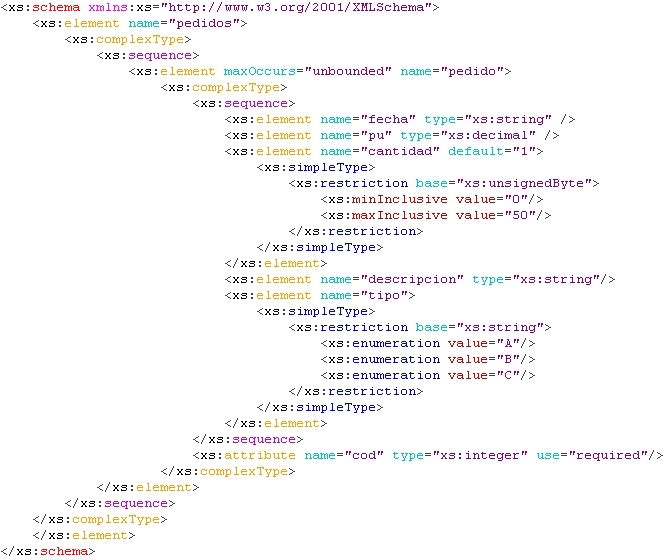
\includegraphics [scale=0.9]{anexos/images/xmltype-database-3-1931043.jpg}
  \end{center}
 \caption[Ejemplo estructura de esquema XML (Documento
 XSD)]{\label{esquemaxml1}Ejemplo estructura de esquema XML (Documento XSD)
 \cite{xml_repo}}
 \end{figure}
%%%%%%%%%%%%%%%%%%%%%%%%%%%%%%%%%%%%%%%%%%%%%%%%%%%%%%%%%%%%%%%%%%
\newpage
\begin{lstlisting}[language=SQL, caption={Ejemplo de registro de esquema
XML en ORACLE \cite{xml_repo}}, label=xml_ora00] 
begin
 DBMS_XMLSCHEMA.REGISTERSCHEMA(SCHEMAURL=>'pedidos.xsd', SCHEMADOC=>'<?xml version="1.0" encoding="utf-8"?>
	<xs:schema xmlns:xs="http://www.w3.org/2001/XMLSchema">
	  <xs:element name="pedidos">
	    <xs:complexType>
	      <xs:sequence>
	        <xs:element maxOccurs="unbounded" name="pedido">
	          <xs:complexType>
	            <xs:sequence>
	              <xs:element name="fecha" type="xs:string" />
        	              <xs:element name="pu" type="xs:decimal" />
	              <xs:element name="cantidad" default="1">
	                 <xs:simpleType>
                                 <xs:restriction base="xs:unsignedByte">
	                         <xs:minInclusive value="0"/>
                                    <xs:maxInclusive value="50"/>
                                </xs:restriction>
	                 </xs:simpleType> </xs:element>
	              <xs:element name="descripcion" type="xs:string"/>
	              <xs:element name="tipo">
	                 <xs:simpleType>
                                 <xs:restriction base="xs:string">
	                            <xs:enumeration value="A"/>
                                    <xs:enumeration value="B"/>
                                    <xs:enumeration value="C"/>
                                </xs:restriction>
	                 </xs:simpleType></xs:element>
	            </xs:sequence>
     		    <xs:attribute name="cod" type="xs:integer" use="required"/>
	          </xs:complexType></xs:element>
	      </xs:sequence>
	    </xs:complexType> </xs:element>
	</xs:schema>', LOCAL=>true, GENTYPES=>false, GENBEAN=>false, GENTABLES=>false, 
    FORCE=>false, OPTIONS=>DBMS_XMLSCHEMA.REGISTER_BINARYXML, OWNER=>USER);
 commit;
end;/
\end{lstlisting} 


\noindent En el c�digo \ref{xml_ora0} se muestra la creaci�n de una tabla con
una columna XMLTYPE. En donde se crea la tabla Reserva que se compone de un
campo llamado pedido de tipo XMLTYPE al cual se le est� especificando que
ser� almacenado como Binary XML. Tambi�n se indica que el campo pedido ser�
validado por el esquema pedidos.xsd que previamente lo ha sido creado. Por otro
lado en el c�digo \ref{xml_ora01} se inserta una tupla en la tabla reserva.\\

\begin{lstlisting}[language=SQL, caption={Ejemplo de creaci�n de tabla con
columna XMLType en ORACLE \cite{xml_repo}}, label=xml_ora0] 
CREATE TABLE FRICCIO.RESERVA(id number, pedido xmltype)
XMLTYPE COLUMN pedido STORE AS BINARY XML
XMLSCHEMA "http://xmlns.oracle.com/xdb/schemas/FRICCIO/pedidos.xsd"
ELEMENT "pedidos";
\end{lstlisting} 



\begin{lstlisting}[language=SQL, caption={Ejemplo de inserci�n en tabla con
columna XMLType en ORACLE \cite{xml_repo}}, label=xml_ora01] 
INSERT INTO friccio.reserva values (1,'<?xml version="1.0"?>
	<pedidos>
		<pedido cod="1">
			<fecha>01-01-2013</fecha>
			<pu>45.5</pu>
			<cantidad>2</cantidad>
			<descripcion>Botella de Vino</descripcion>
			<tipo>C</tipo>
		</pedido>
		<pedido cod="2">
			<fecha>31-12-2012</fecha>
			<pu>25</pu>
			<cantidad>1</cantidad>
			<descripcion>Menu Ejecutivo</descripcion>
			<tipo>A</tipo>
		</pedido>
	</pedidos>');		
\end{lstlisting} 

\noindent Es posible insertar un documento a partir de un archivo XML existente
en el Sistema Operativo o en el XML DB Repository, un ejemplo se describe en el
c�digo \ref{xml_ora02}. \\
\newpage
\begin{lstlisting}[language=SQL, caption={Ejemplo de inserci�n en tabla con
columna XMLType desde archivo existente \cite{xml_repo}}, label=xml_ora02] 
INSERT INTO <tabla> VALUES 
(XMLType(bfilename('<DIR>','<archivo.xml>'),nls_charset_id('AL32UTF8')));
\end{lstlisting} 

\noindent Existen algunas funciones que permiten dar mantenimiento a los
elementos de un documento XML ya registrado. Se har� una demostraci�n de tres de
ellos. Para Agregar un nuevo elemento pedido sobre el documento XML se debe
utilizar la funci�n appendchildxml(), un ejemplo de uso en el c�digo
\ref{xml_ora03}. En el c�digo \ref{xml_ora04}  se modifica el pu (precio
unitario) del nuevo elemento pedido ingresado del valor de 30 a 20 y por �ltimo
en el c�digo \ref{xml_ora05} se elimina el �ltimo elemento ingresado. \\

\begin{lstlisting}[language=SQL, caption={Ejemplo de funci�n AppendChildxml en
ORACLE \cite{xml_repo}}, label=xml_ora03] 
UPDATE reserva set pedido=appendchildxml(pedido,'/pedidos',
	'<pedido cod="3">
		<fecha>31-12-2012</fecha>
		<pu>30</pu>
		<cantidad>1</cantidad>
		<descripcion>xxx</descripcion>
		<tipo>B</tipo>
	</pedido>')
where id=1;
\end{lstlisting} 

\begin{lstlisting}[language=SQL, caption={Ejemplo de UPDATE a columna XMLTYPE
utilizando posiciones en ORACLE \cite{xml_repo}}, label=xml_ora04] 
update reserva set pedido=updatexml(pedido,'/pedidos[1]/pedido[3]/pu/text()',20) 
where id=1;
\end{lstlisting} 

\begin{lstlisting}[language=SQL, caption={Ejemplo de Actualizaci�n eliminando
nodo en columna XMLTYPE ORACLE \cite{xml_repo}}, label=xml_ora05] 
UPDATE reserva set pedido=deletexml(pedido,'/pedidos[1]/pedido[3]');
\end{lstlisting} 

\noindent En el c�digo \ref{ora_xml06} se obtiene el documento XML como String,
en cambio en el c�digo \ref{ora_xml07} como CLOB y en el c�digo \ref{ora_xml08}
se crea un String o CLOB a partir de un contenido.
\newpage
\begin{lstlisting}[language=SQL, caption={Ejemplo de obtenci�n de
documento XML como String en ORACLE \cite{xml_repo}}, label=ora_xml06] 
select id,r.PEDIDO.getStringVal() from reserva r;
\end{lstlisting} 

\begin{lstlisting}[language=SQL, caption={Ejemplo de obtenci�n de
documento XML como Clob en ORACLE \cite{xml_repo}}, label=ora_xml07] 
select id,r.PEDIDO. getClobVal() from reserva r;
\end{lstlisting} 

\begin{lstlisting}[language=SQL, caption={Ejemplo de creaci�n de String o Clob
desde un contenido en ORACLE \cite{xml_repo}}, label=ora_xml08] 
select xmlserialize(DOCUMENT|CONTENT r.PEDIDO as CLOB|VARCHAR|VARCHAR2) from reserva r;
\end{lstlisting} 

\noindent Para obtener nodos espec�ficos de un documento se debe utilizar
XPath. En el ejemplo de la figura \ref{xpath1} se obtienen todos los pu (precios unitarios) de la reserva con
id=1.
En la figura \ref{xpath2} se muestra un ejemplo de c�mo obtener aquellos
pedidos que han superado un precio unitario de 48 de tipo A. Y por �ltimo en el
ejemplo descrito en la figura \ref{xpath3} obtiene aquellos pedidos
cuyo atributo cod sea diferente del valor de 3.

%%%%%%%%%%%%%%%%%%%%%%%%%%%%%%%%%%%%%%%%%%%%%%%%%%%%%%%%%%%%%%%%%%%%%
 \begin{figure}[H]
 \begin{center}
  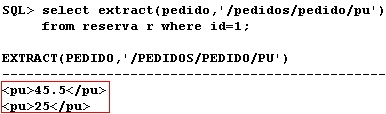
\includegraphics [scale=1]{anexos/images/xmltype-database-16-1931069.jpg}
  \end{center}
 \caption[Ejemplo XPath 1]{\label{xpath1}Ejemplo XPath 1 \cite{xml_repo}}
 \end{figure}
%%%%%%%%%%%%%%%%%%%%%%%%%%%%%%%%%%%%%%%%%%%%%%%%%%%%%%%%%%%%%%%%%%

%%%%%%%%%%%%%%%%%%%%%%%%%%%%%%%%%%%%%%%%%%%%%%%%%%%%%%%%%%%%%%%%%%%%%
 \begin{figure}[H]
 \begin{center}
  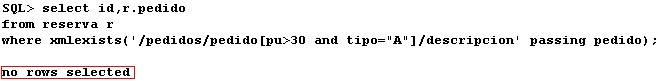
\includegraphics [scale=0.8]{anexos/images/xmltype-database-17-1931070.jpg}
  \end{center}
 \caption[Ejemplo XPath 2]{\label{xpath2}Ejemplo XPath 2 \cite{xml_repo}}
 \end{figure}
%%%%%%%%%%%%%%%%%%%%%%%%%%%%%%%%%%%%%%%%%%%%%%%%%%%%%%%%%%%%%%%%%%

%%%%%%%%%%%%%%%%%%%%%%%%%%%%%%%%%%%%%%%%%%%%%%%%%%%%%%%%%%%%%%%%%%%%%
 \begin{figure}[H]
 \begin{center}
  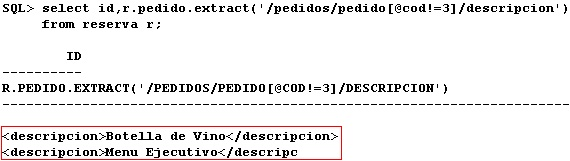
\includegraphics [scale=1]{anexos/images/xmltype-database-18-1931072.jpg}
  \end{center}
 \caption[Ejemplo XPath 3]{\label{xpath3}Ejemplo XPath 3 \cite{xml_repo}}
 \end{figure}
%%%%%%%%%%%%%%%%%%%%%%%%%%%%%%%%%%%%%%%%%%%%%%%%%%%%%%%%%%%%%%%%%%



\subsection{�Como almacenar XML en Oracle?} \label{anexo421}

\subsubsection{�XMLType o tablas relacionales?}

\par \noindent Esta decisi�n inicial puede generalmente estar basada en el
formato de los datos XML y la fidelidad en los requerimientos DOM (Document Object
Model) en el contenido XML. Para el formato, los documentos XML generalmente
pueden ser categorizados como documentos ``centrado en datos'' o ``centrados en
documentos''.

\noindent Los documentos centrados en datos son categorizados por la estructura
regular de los datos, en donde la unidad m�s peque�a es un elemento XML con
contenido simple o un atributo XML. En dicho documento XML, hay poca o ninguna
mezcla de contenido (por ejemplo, etiquetas dentro del contenido de un elemento
XML cadena). Adem�s, la fidelidad DOM del documento no
es requerida de conservar. El c�digo \ref{xml_1} es un ejemplo de
un documento XML centrado en datos.

\noindent 

\begin{lstlisting}[language=xml, caption={Ejemplo de documentos XML centrado
en datos}, label=xml_1] 
<?xml version="1.0"?>
<purchaseOrder orderDate="1999-10-20">
 <shipTo country="US">�</shipTo>
 �<billTo country="US">�</billTo>
	<items>
		<item partNum="872-AA">
 ����		<productName>Lawnmower</productName>
 �����		<quantity>1</quantity>
 ������		<USPrice>148.95</USPrice>
 ������		<comment>Confirm this is electric</comment>
 ����	</item> �
 ��</items>
</purchaseOrder>
\end{lstlisting}

\noindent Todos los datos presentados en el c�digo \ref{xml_1} son representados
como elementos XML o como atributos para elementos XML.

\noindent La mayor�a de los documentos XML centrados en datos son creados
basados en datos relacionales para intercambiar y compartir datos entre aplicaciones.

\noindent Del mismo modo, para documentos centrados en datos, no existe una
necesidad de mantener datos en XML una vez que estos son almacenados en la base
de datos. Si elementos y atributos XML son almacenados correctamente en columnas
de las tablas relacionales, se tiene el almacenamiento optimizado para su
posterior procesamiento, lo que evita la sobrecarga de mantener y gestionar la estructura XML en la base de datos. 
Siempre que se necesite, los datos en XML para el intercambio de datos y la
publicaci�n en la Web, se puede construir Vistas XMLType para envolver los datos
en XML.

\subsubsection{Modelos de almacenamiento XMLType}

\noindent Este tipo de dato abstracto permite almacenar
datos en formato XML, brindando la posibilidad de
utilizar esquemas XML, XPath, XQuery, XSLT, indexaci�n y particionamiento de documentos
XML.
En las versiones anteriores de Oracle Database 9i y 10g los
documentos XML se almacenan como CLOB (Character Large Object) o como
objetos. A partir de la versi�n Oracle Database 11g se
agreg� una nueva posibilidad, almacenarlos en formato
binario (Binary XML), que desde la versi�n 11.2.0.2. es el formato por
defecto \cite{almacenamientoxml}.

\begin{itemize}
  \item \tn{Almacenamiento no estructurado}
  
  Los datos XMLType son almacenados como un tipo CLOB. Los documentos XML son
almacenados preservando el documento original,
inclusive los espacios en blanco. De esta forma, se mantiene
fidelidad de contenido o de documento. Adem�s, Oracle
brinda la posibilidad de asociar un esquema a dicha
forma de almacenamiento. Entrega un muy
bueno desempe�o en las operaciones de inserci�n y recuperaci�n de
documentos completos.
Es una opci�n que proporciona una gran
flexibilidad, pero por otro lado, requiere una sobrecarga
en el procesamiento cuando se necesita consultar su
contenido, como por ejemplo cuando se utilizan
funciones como XMLType.Extract y XMLType.ExistsNode.
Evaluar estas funciones requiere construir el �rbol XML
DOM en memoria y sobre este evaluar las expresiones
XPath. Tambi�n, toda operaci�n de actualizaci�n se debe
realizar a nivel de documento \cite{almacenamientoxml}.
\newpage
\item \tn{Almacenamiento estructurado}

Los datos XMLType son almacenados como
un conjunto de objetos. Los documentos XML
mantienen fidelidad DOM.
Esta alternativa tambi�n es mencionada como
almacenamiento Objeto Relacional (OR) \cite{xml2}.
Es com�n y conveniente almacenarlos con un
esquema asociado, puesto que permite acelerar las consultas y las actualizaciones de granularidad fina. Esto
provoca que las aplicaciones que lo utilizan deban
ajustarse a un esquema de datos bien estructurado y
r�gido.
Por otro lado, presenta varias ventajas en comparaci�n
con el almacenamiento no estructurado. Se logra una
optimizaci�n del manejo de memoria, se reducen los
requerimientos de almacenamiento, y se pueden hacer
actualizaciones a nivel de detalle.
Es necesario mencionar que las mejoras de esta alternativa tiene su
contrapartida, el incremento de la sobrecarga durante la
inserci�n y la recuperaci�n de los datos, adem�s de la
reducci�n de la flexibilidad en t�rminos de estructura \cite{almacenamientoxml}. 

\item \tn{Almacenamiento binario}

Esta forma de almacenamiento provista por la
versi�n 11g es introducida con la intenci�n de compensar
ventajas y desventajas de las dos alternativas anteriores.
As�, provee una gran flexibilidad en cuanto a la
estructura sin deteriorar el desempe�o.
Concretamente, mantiene un buen rendimiento en la
actualizaci�n, indexaci�n y extracci�n de fragmentos; as�
como en las consultas, puesto que parsea el documento
antes de almacenarlo.
La tabla \ref{tablaxml_a1} presenta una comparaci�n muy ilustrativa entre
las tres opciones de almacenamiento descriptas en Oracle 11g \cite{almacenamientoxml}.
\end{itemize}

\subsubsection{Elecci�n de la estructura de almacenamiento}

\begin{table}[H]
    \begin{tabular}{|l|c|c|c|}
    \hline
    ~                          & \tn{CLOB}      & \tn{Objeto Relacional} &
    \tn{XML Binario} \\ \hline Consulta                   & pobre     &
    excelente & bueno / excelente \\ \hline DML                        & pobre     & bueno / excelente & excelente         \\ \hline
    Recuperaci�n de documentos & excelente & bueno / excelente & excelente         \\ \hline
    Flexibilidad de esquema    & bueno     & pobre             & excelente         \\ \hline
    Fidelidad de documento     & excelente & pobre             & bueno / excelente \\ \hline
    \end{tabular}
    \caption[Comparaci�n de los diferentes modelos de
    almacenamiento]{\label{tablaxml_a1}Comparaci�n de los diferentes modelos de
    almacenamiento \cite{almacenamientoxml}}
\end{table}

\noindent Cada modelo de almacenamiento posee un conjunto de
caracter�sticas que lo hacen m�s o menos apropiado
seg�n el tipo de datos a manipular. Sin embargo, aunque
la naturaleza de los datos es un aspecto fundamental a
considerar, el uso que se les dar� a esos datos tambi�n
constituye un factor decisivo.

\begin{itemize}
  \item \tn{Datos Estructurados}
  
  Corresponde a aquellos datos que tienen una estructura
regular y granularidad fina. Los datos contenidos en
facturas de ventas y en cuentas de un banco son
ejemplos de esta categor�a.

	\item \tn{Datos Semiestructurados o No Estructurados}
	
	Se caracterizan por tener una estructura menos regular,
una granularidad m�s gruesa y con contenidos
mezclados; tales como los datos contenidos en correos
electr�nicos, libros, curr�culos y advertencias. En
general, los datos est�n organizados para ser usados por
personas.
Por otra parte, como se coment� con anterioridad, las
aplicaciones que usan los datos tambi�n pueden ser de
diferente naturaleza:
\begin{itemize}
\item \tn{Aplicaciones centradas en datos}

Estas aplicaciones necesitan conocer la estructura de
los datos. En general, los datos son altamente
estructurados. Luego, la aplicaci�n puede tomar ventaja
en este sentido. Es com�n que los datos se ajustan a un
esquema XML.

\item \tn{Aplicaciones centrada en documentos}

En este caso, es com�n que las aplicaciones necesiten
mantener una copia exacta de los documentos, como
sucede por ejemplo en el �mbito judicial, m�dico, etc.
Luego, bajo la hip�tesis de contar con datos
estructurados, por un lado cabe la situaci�n que las
aplicaciones no necesiten conocer esa estructura, y por
otro, que s� lo demanden. En el primer caso, el modelo
de almacenamiento como CLOB ser� la alternativa m�s
aconsejable, mientras que en el segundo, el modelo
apropiado ser�a el binario.
\end{itemize}
\end{itemize}

%\addcontentsline{toc}{chapter}{Documentaci�n caso de estudio}
\chapter{Documentaci�n caso de estudio}




\section{Documentaci�n DER} \label{der}
\noindent \tn{Documentaci�n de entidades}

\begin{table}[H]
\begin{tabular}{|l|p{12.15cm}|}
 \hline
\tn{Nombre:}      & \tn{personal}                                                     
\\ \hline Descripci�n: & Personal del colegio                             
\\ \hline Tipo:        & Normal                                            
\\ \hline Atributos:  & \begin{tabular}{ll}
\underline{rut}: & rut del personal (atributo compuesto \\ 
&  n�mero correlativo y d�gito verificador)\\ 
nombre\_completo: & Nombre completo del personal (atributo \\  
& compuesto consta de nombres, apellido \\
& paterno y materno) \\

 fnac: & Fecha de nacimiento del personal\\ 
edad: & Edad del personal (atributo derivado)\\ 
direccion: & Direcci�n del personal (atributo compuesto \\
&  consta: calle, n�mero, c�digo postal, ciudad \\ & y regi�n) \\ 
celular: & N�meros de celular personal (atributo \\ & multivaluado)\\
mail: & Mails del personal (atributo multivaluado) \end{tabular} \\
\hline
\end{tabular}
\end{table}

\begin{table}[H]
\begin{tabular}{|l|p{12.15cm}|}
 \hline
\tn{Nombre:}      & \tn{docente}                                                               
\\ \hline Descripci�n: & Personal docente del colegio                                  
\\ \hline Tipo:       & Especializaci�n de personal                                                     
\\ \hline Atributos:   & \begin{tabular}{ll}
cant\_cursos: & Cantidad de cursos en que hace clases (atributo \\
& derivado) \end{tabular} \\ \hline
\end{tabular}
\end{table}

\begin{table}[H]
\begin{tabular}{|l|p{12.15cm}|}
 \hline
\tn{Nombre: }     & \tn{no\_docente}                                                               
\\ \hline Descripci�n: & Personal no docente del colegio                                  
\\ \hline Tipo:        & Especializaci�n de personal                                                     
\\ \hline Atributos:   & No tiene \\ \hline
\end{tabular}
\end{table}



\begin{table}[H]
\begin{tabular}{|l|p{12.15cm}|}
 \hline
\tn{Nombre:}      & \tn{cargo}                                                              
\\ \hline Descripci�n: & Cargo que posee el personal no docente                                  
\\ \hline Tipo:        & Normal                                                     
\\ \hline Atributos:   & \begin{tabular}{ll}
\underline{id\_cargo}: & C�digo identificador del cargo \\
nom\_c: & Nombre del cargo \\
desc\_c: & Descripci�n del cargo\\
\end{tabular} \\ \hline
\end{tabular}
\end{table}


\begin{table}[H]
\begin{tabular}{|l|p{12.15cm}|}
 \hline
\tn{Nombre:}      & \tn{nivel}                                                              
\\ \hline Descripci�n: & Nivel de ense�anza de un curso por ejemplo
1ero b�sico, 2do medio, etc.
 \\ \hline Tipo:        & Normal                                                     
\\ \hline Atributos:   & \begin{tabular}{ll}
\underline{id\_nivel}: & C�digo identificador del nivel \\
nom\_niv: & Nombre del nivel\\
\end{tabular} \\ \hline
\end{tabular}
\end{table}

\begin{table}[H]
\begin{tabular}{|l|p{12.15cm}|}
 \hline
\tn{Nombre:}      & \tn{curso}                                                              
\\ \hline Descripci�n: & Curso del colegio por ejemplo 1ero b�sico A,
2do medio B, etc.
 \\ \hline Tipo:        & D�bil con respecto a nivel, agregaci�n
 compuesta por \\ & curso, asignatura y relacionamiento curso\_asignatura
  \\ \hline Atributos:   & \begin{tabular}{ll}
\underline le\underline tr\underline a: & Letra identificadora del
curso \\
a�o: & A�o del curso por ejemplo 1ero b�sico A 2013, \\
& 2do medio B 2011 \\
\end{tabular} \\ \hline
\end{tabular}
\end{table}



\begin{table}[H]
\begin{tabular}{|l|p{12.15cm}|}
 \hline
\tn{Nombre: }     & \tn{asignatura}                                                           
\\ \hline Descripci�n: & Asignatura dictada en un curso en particular
 \\ \hline Tipo:        & Normal, agregaci�n compuesta por
 \\ & curso, asignatura y relacionamiento curso\_asignatura                                                  
\\ \hline Atributos:   & \begin{tabular}{ll}
\underline{id\_asig}: & C�digo identificador de la asignatura \\
nom\_asig: & Nombre de la asignatura\\
\end{tabular} \\ \hline
\end{tabular}
\end{table}

\begin{table}[H]
\begin{tabular}{|l|p{12.15cm}|}
 \hline
\tn{Nombre:}      & \tn{programa\_tipo}                                                              
\\ \hline Descripci�n: & Tipo de programa educacional ejemplo: Unidad,
Aprendizaje esperado, etc.
 \\ \hline Tipo:        & Normal \\ \hline 
 Atributos:  
& \begin{tabular}{ll} \underline{id\_tp}: & C�digo identificador del
tipo de programa
\\
nom\_pt: & Nombre del tipo de programa\\
abrev: & Abreviatura del tipo de programa Ej: U, AE, OFT, etc.
\end{tabular} \\ \hline
\end{tabular}
\end{table}

\begin{table}[H]
\begin{tabular}{|l|p{12.15cm}|}
 \hline
\tn{Nombre:}      & \tn{detalle\_programa}                                                              
\\ \hline Descripci�n: & Detalle del programa educacional de una
asignatura
\\
& ejemplo: Sumas y restas (unidad, 1ero b�sico).
 \\ \hline Tipo:        & Normal \\ \hline 
 Atributos:  
& \begin{tabular}{ll} \underline{id\_dp}: & C�digo identificador del
detalle de programa
\\
nomdp: & Nombre del detalle de programa, ejemplo unidad1\\
desc\_dp: & Descripci�n por ejemplo ``Sumas y restas''\\
\end{tabular} \\ \hline
\end{tabular}
\end{table}


\begin{table}[H]
\begin{tabular}{|l|p{12.15cm}|}
 \hline
\tn{Nombre:}      & \tn{planificacion }                                                             
\\ \hline Descripci�n: & Planificaci�n realizada por un docente para
una asignatura\\
& de un curso en particular
 \\ \hline Tipo:        & Normal \\ \hline 
 Atributos:  
& \begin{tabular}{ll} \underline{id\_plan}: & C�digo identificador de
la planificaci�n
\\
tipo\_plan: & Tipo de planificaci�n: Anual, por unidad o por clase \\
fcreacion: & Fecha de creaci�n de la planificaci�n\\
ult\_estado: & �ltimo estado por el que paso la planificaci�n\\
ult\_modif: & Fecha de la �ltima modificaci�n de la planificaci�n\\
\end{tabular} \\ \hline
\end{tabular}
\end{table}


\begin{table}[H]
\begin{tabular}{|l|p{12.15cm}|}
 \hline
\tn{Nombre:}      & \tn{estado }                                                             
\\ \hline Descripci�n: & Estados por los que pasa una planificaci�n\\
  \hline Tipo:        & Normal \\ \hline 
Atributos:  
& \begin{tabular}{ll} \underline{id\_estado}: & C�digo identificador
del estado\\
nom\_estado: & Nombre del estado por ejemplo: Vigente, \\
&	rechazado, borrador\\
\end{tabular} \\ \hline
\end{tabular}
\end{table}

\begin{table}[H]
\begin{tabular}{|l|p{12.15cm}|}
 \hline
\tn{Nombre:}      & \tn{plan\_anual}                   
\\ \hline Descripci�n: & Planificaci�n del tipo anual realizada por un
docente para una asignatura de un curso en particular
 \\ \hline Tipo:        & Especializaci�n de planificaci�n \\ \hline 
 Atributos: & No tiene \\ \hline
\end{tabular}
\end{table}


\begin{table}[H]
\begin{tabular}{|l|p{12.15cm}|}
 \hline
\tn{Nombre:}      & \tn{plan\_unidad}                                                            
\\ \hline Descripci�n: & Planificaci�n  del tipo por unidad realizada
por un docente para una asignatura de un curso en particular
 \\ \hline Tipo:        & Especializaci�n de planificaci�n \\ \hline 
 Atributos: & No tiene \\ \hline
\end{tabular}
\end{table}


\begin{table}[H]
\begin{tabular}{|l|p{12.15cm}|}
 \hline
\tn{Nombre:}      & \tn{plan\_clase}                                                           
\\ \hline Descripci�n: & Planificaci�n  del tipo clase a clase
realizada por un docente para una asignatura 
 de un curso en particular
 \\ \hline Tipo:        & Especializaci�n de planificaci�n \\ \hline 
 Atributos: & No tiene \\ \hline
\end{tabular}
\end{table}

\begin{table}[H]
\begin{tabular}{|l|p{12.15cm}|}
 \hline
\tn{Nombre:}      & \tn{periodo}                                                           
\\ \hline Descripci�n: & periodos (de tiempo) de una planificaci�n
anual\\
 \hline Tipo:        & Normal \\ \hline 
 Atributos: &  \begin{tabular}{ll} \underline{id\_periodo}: &
 C�digo identificador del periodo\\
mes\_ini: & Mes de inicio del periodo\\
mes\_ter: & Mes de t�rmino del periodo\\
duracion: & Duraci�n del periodo en horas\\
aprevios: & Aprendizajes previos que debe poseer el curso \\
& (atributo
multivaluado)\end{tabular} \\ \hline
\end{tabular}
\end{table}

\begin{table}[H]
\begin{tabular}{|l|p{12.15cm}|}
 \hline
\tn{Nombre:}      & \tn{unidad}                                                           
\\ \hline Descripci�n: & unidades (a pasar) en una planificaci�n por
unidad\\
 \hline Tipo:       & Normal \\ \hline 
 Atributos: &  \begin{tabular}{ll} \underline{id\_unidad}: &
 C�digo identificador de la unidad\\
fechai: & Fecha de inicio de la unidad\\
fechat: & Fecha de t�rmino de la unidad\\
duracion: & Duraci�n del periodo en horas\\
aprevios: & Aprendizajes previos que debe poseer el curso \\
& (atributo multivaluado) \end{tabular} \\ \hline
\end{tabular}
\end{table}

\begin{table}[H]
\begin{tabular}{|l|p{12.15cm}|}
 \hline
\tn{Nombre:}      & \tn{clase}                                                           
\\ \hline Descripci�n: & clases de una planificaci�n clase a clase\\
 \hline Tipo:        & Normal \\ \hline 
 Atributos: &  \begin{tabular}{ll} \underline{id\_clase}: & C�digo
 identificador de la clase\\
fecha: & Fecha en que se realizar� la clase\\
horario: & horario en que se har� la clase (atributo compuesto \\
& consta de d�a, hora inicio, hora t�rmino y duraci�n)\\
aprevios: & Aprendizajes previos que debe poseer el curso \\
& (atributo multivaluado) \end{tabular} \\ \hline
\end{tabular}
\end{table}

\begin{table}[H]
\begin{tabular}{|l|p{12.15cm}|}
 \hline
\tn{Nombre:}      & \tn{metodologia}                                                           
\\ \hline Descripci�n: & metodolog�a a emplear en un periodo, unidad o
actividad\\
 \hline Tipo:        & Normal \\ \hline 
 Atributos: &  \begin{tabular}{ll} \underline{id\_met}: & C�digo
 identificador de la metodolog�a\\
nom\_met: & Nombre de la metodolog�a\\
desc\_met: & Descripci�n de la metodolog�a \end{tabular} \\ \hline
\end{tabular}
\end{table}


\begin{table}[H]
\begin{tabular}{|l|p{12.15cm}|}
 \hline
\tn{Nombre:}      & \tn{recurso}                                                           
\\ \hline Descripci�n: & recurso a utilizar en un periodo, unidad o
actividad\\
 \hline Tipo:        & Normal \\ \hline 
 Atributos: &  \begin{tabular}{ll} \underline{id\_rec}: & C�digo
 identificador del recurso\\
nom\_rec: & Nombre del recurso\\
desc\_rec: & Descripci�n del recurso \end{tabular} \\ \hline
\end{tabular}
\end{table}

\begin{table}[H]
\begin{tabular}{|l|p{12.15cm}|}
 \hline
\tn{Nombre:}      & \tn{actividad}                                                           
\\ \hline Descripci�n: & actividad a realizar en una clase\\
 \hline Tipo:        & Normal \\ \hline 
 Atributos: &  \begin{tabular}{ll} \underline{id\_act}: & C�digo
 identificador de la actividad\\
desc\_act: & Descripci�n de la actividad \\
duracion: & Duraci�n de la actividad \end{tabular} \\ \hline
\end{tabular}
\end{table}

\par \noindent \tn{Documentaci�n de los relacionamientos}

\begin{table}[H]
\begin{tabular}{|l|p{9.85cm}|}
 \hline
\tn{Nombre:}      & \tn{curso\_asignatura}  \\ \hline 
Tipo:        & Normal \\ \hline 
Entidades que participan:	& curso \\ 
&	asignatura\\
\hline
Cardinalidad: 	& 1 curso tiene muchas asignaturas\\
&	1 asignatura pertenece s�lo a 1 curso\\
 \hline
Atributos: 	& No tiene\\ \hline
\end{tabular}
\end{table}

\begin{table}[H]
\begin{tabular}{|l|p{9.85cm}|}
 \hline
\tn{Nombre:}      & \tn{jefe}  \\ \hline 
Descripci�n: & Profesor jefe del curso\\ \hline 
Tipo:        & Normal \\ \hline 
Entidades que participan:	& docente \\ 
&	curso \\
\hline
Cardinalidad: 	& 1 curso tiene s�lo un profesor jefe\\
&	1 profesor puede ser profesor jefe de 0 o 1 curso\\
 \hline
Atributos: 	& No tiene\\ \hline
\end{tabular}
\end{table}


\begin{table}[H]
\begin{tabular}{|l|p{9.85cm}|}
 \hline
\tn{Nombre:}      & \tn{nivel\_curso}  \\ \hline 
Descripci�n: & Nivel de ense�anza al que pertenece el curso\\ \hline 
Tipo:        & D�bil \\ \hline 
Entidades que participan:	& nivel \\ 
&	curso \\
\hline
Cardinalidad: 	& 1 curso tiene s�lo 1 nivel\\
&	1 nivel puede tener muchos cursos\\
 \hline
Atributos: 	& No tiene\\ \hline
\end{tabular}
\end{table}

\begin{table}[H]
\begin{tabular}{|l|p{9.85cm}|}
 \hline
\tn{Nombre:}      & \tn{no\_docente\_cargo}  \\ \hline 
Descripci�n: & Cargo que posee el no docente\\ \hline 
Tipo:        & Normal \\ \hline 
Entidades que participan:	& no\_docente \\ 
&	cargo \\
\hline
Cardinalidad: 	& 1 no docente tiene s�lo un cargo\\
&	1 cargo puede tener asociado 1 o m�s no docentes\\
 \hline
Atributos: 	& No tiene\\ \hline
\end{tabular}
\end{table}

\begin{table}[H]
\begin{tabular}{|l|p{9.85cm}|}
 \hline
\tn{Nombre:}      & \tn{detalle\_programa\_asignatura} \\ \hline 
Descripci�n: & Asignatura a la que pertenece el detalle de programa\\
\hline Tipo:        & Normal \\ \hline 
Entidades que participan:	& detalle\_programa \\ 
&	asignatura \\
\hline
Cardinalidad: 	& 1 detalle de programa tiene s�lo una asignatura\\
&	1 asignatura puede tener asociado 1 o m�s detalles de programas\\
 \hline
Atributos: 	& No tiene\\ \hline
\end{tabular}
\end{table}

\begin{table}[H]
\begin{tabular}{|l|p{9.85cm}|}
 \hline
\tn{Nombre:}      & \tn{detalle\_programa\_programa\_tipo}  \\ \hline 
Descripci�n: & Tipo de programa al que pertenece el detalle de
programa\\
\hline Tipo:        & Normal \\ \hline 
Entidades que participan:	& detalle\_programa \\ 
&	programa\_tipo \\
\hline
Cardinalidad: 	& 1 detalle de programa tiene s�lo un tipo de
programa\\
&	1 tipo de programa puede tener asociado 1 o m�s detalles de programa\\
 \hline
Atributos: 	& No tiene\\ \hline
\end{tabular}
\end{table}

\begin{table}[H]
\begin{tabular}{|l|p{9.85cm}|}
 \hline
\tn{Nombre:}      & \tn{crea}  \\ \hline 
Descripci�n: & Un docente crea una planificaci�n\\ \hline 
Tipo:        & Normal \\ \hline 
Entidades que participan:	& planificacion\\ 
&	docente \\
\hline
Cardinalidad: 	& 1 planificaci�n tiene s�lo un docente\\
&	1 docente puede crear 1 o m�s planificaciones\\
 \hline
Atributos: 	& No tiene\\ \hline
\end{tabular}
\end{table}

\begin{table}[H]
\begin{tabular}{|l|p{9.85cm}|}
 \hline
\tn{Nombre: }     & \tn{planificacion\_estado}  \\ \hline 
Descripci�n: & Estados por los que pasa una planificaci�n\\ \hline 
Tipo:        & Normal \\ \hline 
Entidades que participan:	& planificacion \\ 
&	estado\\
\hline
Cardinalidad: 	& 1 planificaci�n puede pasar por muchos estados\\
&	1 estado puede estar asociado a 1 o m�s planificaciones\\
 \hline
Atributos: &  \begin{tabular}{ll} fcambio: & Fecha cambio de
estado (atributo \\ & multivaluado)  \end{tabular}
\\ \hline
\end{tabular}
\end{table}

\begin{table}[H]
\begin{tabular}{|l|p{9.85cm}|}
 \hline
\tn{Nombre: }     & \tn{evaluacion}  \\ \hline 
Descripci�n: & Un no docente eval�a si una planificaci�n si esta
correcta\\
\hline Tipo:        & Normal \\ \hline 
Entidades que participan:	& planificacion \\ 
&	no\_docente\\
\hline
Cardinalidad: 	& 1 planificaci�n puede ser evaluada muchas veces por un
no docente\\
&	1 no docente puede evaluar muchas veces una planificaci�n\\
 \hline
Atributos: &  \begin{tabular}{ll} EvaDetalle: & Detalle de la
evaluaci�n (atributo \\ & multivaluado compuesto, consta de \\ & fecha de
evaluaci�n y un comentario) \end{tabular} \\ \hline
\end{tabular}
\end{table}


\begin{table}[H]
\begin{tabular}{|l|p{9.85cm}|}
 \hline
\tn{Nombre:}      & \tn{plan\_anual\_periodo}  \\ \hline 
Descripci�n: & Una planificaci�n anual posee periodos\\ \hline 
Tipo:        & Normal \\ \hline 
Entidades que participan:	& plan\_anual\\ 
&	periodo \\
\hline
Cardinalidad: 	& 1 periodo pertenece s�lo a una planificaci�n anual\\
&	1 planificaci�n anual puede tener 1 o m�s periodos\\
 \hline
Atributos: 	& No tiene\\ \hline
\end{tabular}
\end{table}

\begin{table}[H]
\begin{tabular}{|l|p{9.85cm}|}
 \hline
\tn{Nombre:}      & \tn{plan\_unidad\_unidad}  \\ \hline 
Descripci�n: & Una planificaci�n por unidad posee unidades\\ \hline 
Tipo:        & Normal \\ \hline 
Entidades que participan:	& plan\_unidad\\ 
&	unidad \\
\hline
Cardinalidad: 	& 1 unidad pertenece s�lo a una planificaci�n por
unidad\\
&	1 planificaci�n por unidad puede tener 1 o m�s unidades\\
 \hline
Atributos: 	& No tiene\\ \hline
\end{tabular}
\end{table}

\begin{table}[H]
\begin{tabular}{|l|p{9.85cm}|}
 \hline
\tn{Nombre:}      & \tn{plan\_clase\_clase}  \\ \hline 
Descripci�n: & Una planificaci�n clase a clase posee clases\\ \hline 
Tipo:        & Normal \\ \hline 
Entidades que participan:	& plan\_clase\\ 
&	clase \\
\hline
Cardinalidad: 	& 1 clase pertenece s�lo a una planificaci�n clase a
clase\\
&	1 planificaci�n clase a clase puede tener 1 o m�s clases\\
 \hline
Atributos: 	& No tiene\\ \hline
\end{tabular}
\end{table}

\begin{table}[H]
\begin{tabular}{|l|p{9.85cm}|}
 \hline
\tn{Nombre:}      & \tn{clase\_actividad}  \\ \hline 
Descripci�n: & Actividades a realizar en una clase\\ \hline 
Tipo:        & Normal \\ \hline 
Entidades que participan:	& clase\\ 
&	actividad \\
\hline
Cardinalidad: 	& 1 actividad pertenece s�lo a una clase\\
&	1 clase puede realizar 1 o m�s actividades\\
 \hline
Atributos: 	& No tiene\\ \hline
\end{tabular}
\end{table}


\begin{table}[H]
\begin{tabular}{|l|p{9.85cm}|}
 \hline
\tn{Nombre:}      & \tn{clase\_detalle\_programa}  \\ \hline 
Descripci�n: & En una clase se ense�ar�n detalles de programas
educacionales\\
\hline Tipo:        & Normal \\ \hline 
Entidades que participan:	& clase\\ 
&	detalle\_programa \\
\hline
Cardinalidad: 	& En 1 clase se pueden ense�ar muchos detalles de
programa\\
&	1 detalle de programa puede ser ense�ado en 1 o m�s clases\\
 \hline
Atributos: 	& No tiene\\ \hline
\end{tabular}
\end{table}

\begin{table}[H]
\begin{tabular}{|l|p{9.85cm}|}
 \hline
\tn{Nombre:}      & \tn{periodo\_detalle\_programa}  \\ \hline 
Descripci�n: & En un periodo se ense�ar�n detalles de programas
educacionales\\
\hline Tipo:       & Normal \\ \hline 
Entidades que participan:	& periodo\\ 
&	detalle\_programa \\
\hline
Cardinalidad: 	& En 1 periodo se pueden ense�ar muchos detalles de
programa\\
&	1 detalle de programa puede ser ense�ado en 1 o m�s periodos\\
 \hline
Atributos: 	& No tiene\\ \hline
\end{tabular}
\end{table}

\begin{table}[H]
\begin{tabular}{|l|p{9.85cm}|}
 \hline
\tn{Nombre:}      & \tn{unidad\_detalle\_programa}  \\ \hline 
Descripci�n: & En una unidad se ense�ar�n detalles de programas
educacionales\\
\hline Tipo:        & Normal \\ \hline 
Entidades que participan:	& unidad\\ 
&	detalle\_programa \\
\hline
Cardinalidad: 	& En 1 unidad se pueden ense�ar muchos detalles de
programa\\
&	1 detalle de programa puede ser ense�ado en 1 o m�s unidades\\
 \hline
Atributos: 	& No tiene\\ \hline
\end{tabular}
\end{table}

\begin{table}[H]
\begin{tabular}{|l|p{9.85cm}|}
 \hline
\tn{Nombre:}     & \tn{unidad\_metodologia}  \\ \hline 
Descripci�n: & En una unidad se aplicar�n metodolog�as de ense�anza\\
\hline Tipo:        & Normal \\ \hline 
Entidades que participan:	& unidad\\ 
&	metodologia \\
\hline
Cardinalidad: 	& En 1 unidad se pueden emplear muchas metodolog�as\\
&	1 metodolog�a puede ser aplicada en 1 o m�s unidades\\
 \hline
Atributos: 	& No tiene\\ \hline
\end{tabular}
\end{table}

\begin{table}[H]
\begin{tabular}{|l|p{9.85cm}|}
 \hline
\tn{Nombre:}      & \tn{periodo\_metodologia}  \\ \hline 
Descripci�n: & En un periodo se aplicar�n metodolog�as de ense�anza\\
\hline Tipo:        & Normal \\ \hline 
Entidades que participan:	& periodo\\ 
&	\metodologia \\
\hline
Cardinalidad: 	& En 1 periodo se pueden emplear muchas metodolog�as\\
&	1 metodolog�a puede ser aplicada en 1 o m�s periodos\\
 \hline
Atributos: 	& No tiene\\ \hline
\end{tabular}
\end{table}

\begin{table}[H]
\begin{tabular}{|l|p{9.85cm}|}
 \hline
\tn{Nombre:}      & \tn{unidad\_recurso}  \\ \hline 
Descripci�n: & En una unidad se puede utilizar recursos educativos\\
\hline Tipo:        & Normal \\ \hline 
Entidades que participan:	& unidad\\ 
&	recurso \\
\hline
Cardinalidad: 	& En 1 unidad se pueden utilizar muchos recursos
educativos\\
&	1 recurso puede ser utilizado en 1 o m�s unidades\\
 \hline
Atributos: 	& No tiene\\ \hline
\end{tabular}
\end{table}

\begin{table}[H]
\begin{tabular}{|l|p{9.85cm}|}
 \hline
\tn{Nombre:}      & \tn{periodo\_recurso}  \\ \hline 
Descripci�n: & En un periodo se puede utilizar recursos educativos\\
\hline Tipo:        & Normal \\ \hline 
Entidades que participan:	& periodo\\ 
&	recurso \\
\hline
Cardinalidad: 	& En 1 periodo se pueden utilizar muchos recursos
educativos\\
&	1 recurso puede ser utilizado en 1 o m�s periodos\\
 \hline
Atributos: 	& No tiene\\ \hline
\end{tabular}
\end{table}

\begin{table}[H]
\begin{tabular}{|l|p{9.85cm}|}
 \hline
\tn{Nombre:}      & \tn{actividad\_recurso}  \\ \hline 
Descripci�n: & En una actividad se puede utilizar recursos
educativos\\
\hline Tipo:       & Normal \\ \hline 
Entidades que participan:	& actividad\\ 
&	recurso \\
\hline
Cardinalidad:	& En 1 actividad se pueden utilizar muchos recursos
educativos\\
&	1 recurso puede ser utilizado en 1 o m�s actividades\\
 \hline
Atributos: 	& No tiene\\ \hline
\end{tabular}
\end{table}

\begin{table}[H]
\begin{tabular}{|l|p{9.85cm}|}
 \hline
\tn{Nombre:}      & \tn{actividad\_metodologia}  \\ \hline 
Descripci�n: & En una actividad se aplicar�n metodolog�as de
ense�anza\\
\hline Tipo:        & Normal \\ \hline 
Entidades que participan:	& actividad\\ 
&	metodologia \\
\hline
Cardinalidad: 	& En 1 actividad se pueden emplear muchas
metodolog�as\\
&	1 metodolog�a puede ser aplicada en 1 o m�s actividades\\
 \hline
Atributos: 	& No tiene\\ \hline
\end{tabular}
\end{table}

\begin{table}[H]
\begin{tabular}{|l|p{9.85cm}|}
 \hline
\tn{Nombre:}      & \tn{curso\_asignatura\_docente}  \\ \hline 
Descripci�n: & Un docente dicta una asignatura en un curso
espec�fico\\
\hline Tipo:        & Normal \\ \hline 
Entidades que participan:	& curso\\ 
&	asignatura \\
&	docente	\\
\hline
Cardinalidad: 	& En un 1 curso hay muchas asignaturas que son dictadas
por 1 docente\\
&	Muchas asignaturas pertenecen a 1 curso y es dictada por 1 docente\\
&	1 docente puede dictar muchas asignaturas de 1 curso \\
 \hline
Atributos: 	& No tiene\\ \hline
\end{tabular}
\end{table}


\begin{table}[H]
\begin{tabular}{|l|p{9.85cm}|}
 \hline
\tn{Nombre:}      & \tn{curso\_asignatura\_planificacion}  \\ \hline 
Descripci�n: & Se crean planificaciones para una asignatura de un curso
en espec�fico\\
\hline Tipo:        & Normal \\ \hline 
Entidades que participan:	& curso\\ 
&	asignatura \\
&	planificacion	\\
\hline
Cardinalidad: 	& En un 1 curso hay muchas asignaturas de las que se
pueden crear muchas planificaciones\\
&	1 asignatura de 1 curso en particular puede tener muchas planificaciones
asociadas\\
&	1 planificaci�n es creada para 1  asignatura de 1 curso en particular
\\
 \hline
Atributos: 	& No tiene\\ \hline
\end{tabular}
\end{table}

\section{Documentaci�n modelo relacional} \label{docrelacional}

\par \noindent \tn{Documentaci�n de tablas} \\

\noindent \tn{Nombre Tabla: nivel}
\begin{table}[H]
\begin{tabular}{|p{4.5cm}|p{2.5cm}|p{1cm}|p{1.5cm}|p{3.55cm}|}
 \hline
\tn{Nombre atributo}      & \tn{Tipo dato} & \tn{PK FK} & \tn{Nulo �nico} &
\tn{Documentaci�n}\\ \hline id\_nivel	& number	&	PK		&	NN,U 	& Identificador de
nivel de ense�anza \\ \hline nom\_nivel		&	varchar(30)	&			&	NN	
&
Nombre del nivel de ense�anza
\\
\hline
\end{tabular}
\end{table}

\noindent \tn{Nombre Tabla: programa\_tipo}
\begin{table}[H]
\begin{tabular}{|p{4.5cm}|p{2.5cm}|p{1cm}|p{1.5cm}|p{3.55cm}|}
 \hline
\tn{Nombre atributo}      & \tn{Tipo dato} & \tn{PK FK} & \tn{Nulo �nico} & \tn{Documentaci�n}\\ \hline
id\_pt	& \tn{number}	&	PK		&	NN,U 	& Identificador de
tipo de programa \\ \hline 
nom\_pt		&	varchar2(30)	&			&	NN	
&
Nombre del tipo de programa
\\
\hline
abrev		&	varchar2(10)	&			&	NN
&
Abreviatura de tipo de programa
\\
\hline
\end{tabular}
\end{table}

\noindent \tn{Nombre Tabla: curso}
\begin{table}[H]
\begin{tabular}{|p{4.5cm}|p{2.5cm}|p{1cm}|p{1.5cm}|p{3.55cm}|}
 \hline
\tn{Nombre atributo}      & \tn{Tipo dato} & \tn{PK FK} & \tn{Nulo �nico} &
\tn{Documentaci�n}\\ \hline id\_nivel	& number	&	PK  FK1		&	NN,U 	& Identificador de
nivel de ense�anza del curso \\ \hline 
letra		&	char(1)	&	PK			&	NN	
&
Letra del curso
\\
\hline
year		&	number	&			&	NN	
&
A�o del curso
\\
\hline
num\_correlativo	& number	&	FK2		&	NN,U 	& n�mero de rut
del profesor jefe \\ \hline dv		&	char(1)	&	FK2		&	NN		&
d�gito verificador del profesor jefe \\ \hline
\end{tabular}
\end{table}



\noindent \tn{Nombre Tabla: personal}
\begin{table}[H]
\begin{tabular}{|p{4.5cm}|p{2.5cm}|p{1cm}|p{1.5cm}|p{3.55cm}|}
 \hline
\tn{Nombre atributo}      & \tn{Tipo dato} & \tn{PK FK} & \tn{Nulo �nico} &
\tn{Documentaci�n}\\ \hline
num\_correlativo	& number	&	PK		&	NN,U 	& n�mero de rut
\\ \hline dv		&	char(1)	&	PK		&	NN		&	d�gito verificador \\ \hline
nombres		&	varchar2(50)	&			&	NN 	&	Nombres  de la
persona \\ \hline
apaterno		&	varchar2(30)	&		&	NN		&	Apellido
parterno de la persona \\ \hline
amaterno		&	varchar2(30)	&		&	NN		&	Apellido
materno de la persona \\ \hline
fnac		&	date	&		&	NN		&	Fecha de nacimiento de la
persona \\ \hline 
calle		&	varchar2(30)	&			&	NN		&	Calle de la
direcci�n de la persona \\ \hline
num		&	varchar2(10)	&			&	NN		&	N�mero de la
direcci�n de la persona \\ \hline
cod\_postal		&	varchar2(10)	&			&	NN		&	C�digo postal de la
direcci�n de la persona \\ \hline
ciudad		&	varchar2(30)	&			&	NN		&	Ciudad donde vive la
persona \\ \hline
region		&	varchar2(30)	&			&	NN	&	Regi�n donde vive la
persona 
\\
\hline
\end{tabular}
\end{table}

\noindent \tn{Nombre Tabla: personalmail}
\begin{table}[H]
\begin{tabular}{|p{4.5cm}|p{2.5cm}|p{1cm}|p{1.5cm}|p{3.55cm}|}
 \hline
\tn{Nombre atributo}      & \tn{Tipo dato} & \tn{PK FK} & \tn{Nulo �nico} &
\tn{Documentaci�n}\\ \hline num\_correlativo	& number	&	PK  FK		&	NN,U 	& n�mero
de rut \\ \hline dv		&	char(1)	&	PK, FK		&	NN		&	d�gito
verificador \\ \hline mail		&	varchar2(100)	&		PK	&	NN		&	Correo  de la
persona
\\
\hline
\end{tabular}
\end{table}

%\newpage

\noindent \tn{Nombre Tabla: personalcelular}
\begin{table}[H]
\begin{tabular}{|p{4.5cm}|p{2.5cm}|p{1cm}|p{1.5cm}|p{3.55cm}|}
 \hline
\tn{Nombre atributo}      & \tn{Tipo dato} & \tn{PK FK} & \tn{Nulo �nico} &
\tn{Documentaci�n}\\ \hline num\_correlativo	& number	&	PK, FK		&	NN,U 	& n�mero
de rut \\ \hline dv		&	char(1)	&	PK  FK		&	NN		&	d�gito
verificador \\ \hline celular		&	number	&		PK	&	NN	
&
Celular  de la persona
\\
\hline
\end{tabular}
\end{table}

\noindent \tn{Nombre Tabla: detalle\_programa}
\begin{table}[H]
\begin{tabular}{|p{4.5cm}|p{2.5cm}|p{1cm}|p{1.5cm}|p{3.55cm}|}
 \hline
\tn{Nombre atributo}      & \tn{Tipo dato} & \tn{PK FK} & \tn{Nulo �nico} &
\tn{Documentaci�n}\\ \hline id\_dp	& number	&	PK		&	NN,U 	& Identificador de
detalle de programa \\ \hline 
nom\_dp		&	varchar2(50)	&			&	NN	
&
Nombre del detalle de programa
\\
\hline
desc\_dp		&	varchar2 (1000)	&			&	NN	
&
Descripci�n del detalle de programa
\\
\hline
id\_pt	& number	&	FK1		&	NN,U 	& Identificador de
tipo de programa \\ \hline 
id\_asig	& number	&	FK2		&	NN,U 	& Identificador de
de la asignatura del detalle de programa \\ \hline 
\end{tabular}
\end{table}





\noindent \tn{Nombre Tabla: docente}
\begin{table}[H]
\begin{tabular}{|p{4.5cm}|p{2.5cm}|p{1cm}|p{1.5cm}|p{3.55cm}|}
 \hline
\tn{Nombre atributo}      & \tn{Tipo dato} & \tn{PK FK} & \tn{Nulo �nico} &
\tn{Documentaci�n}\\ \hline personal\_num\_correlativo	& number	&	PK  FK		&	NN,U
& n�mero de rut \\ \hline 
personal\_dv		&	char(1)	&	PK, FK		&
NN & d�gito verificador \\ \hline
\end{tabular}
\end{table}


\noindent \tn{Nombre Tabla: no\_docente}
\begin{table}[H]
\begin{tabular}{|p{4.5cm}|p{2.5cm}|p{1cm}|p{1.5cm}|p{3.55cm}|}
 \hline
\tn{Nombre atributo}      & \tn{Tipo dato} & \tn{PK FK} & \tn{Nulo �nico} &
\tn{Documentaci�n}\\ \hline personal\_num\_correlativo	& number	&	PK  FK1		&
NN,U 	& n�mero de rut \\ \hline personal\_dv		&	char(1)	&	PK  FK1		&
NN & d�gito verificador \\ \hline
id\_cargo		&	number	&	FK2		&
NN & Identificador del cargo del no docente \\ \hline
\end{tabular}
\end{table}


\noindent \tn{Nombre Tabla: cargo}
\begin{table}[H]
\begin{tabular}{|p{4.5cm}|p{2.5cm}|p{1cm}|p{1.5cm}|p{3.55cm}|}
 \hline
\tn{Nombre atributo}      & \tn{Tipo dato} & \tn{PK FK} & \tn{Nulo �nico} &
\tn{Documentaci�n}\\ \hline id\_cargo	& number	&	PK	&	NN,U 	&
Identificador del cargo \\ \hline 
nom\_c		&
varchar2(30) &  & NN & Nombre del cargo \\ \hline
desc\_c		&	varchar2(500)	&			&
NN & Descripci�n del cargo \\ \hline
\end{tabular}
\end{table}

\noindent \tn{Nombre Tabla: estado}
\begin{table}[H]
\begin{tabular}{|p{4.5cm}|p{2.5cm}|p{1cm}|p{1.5cm}|p{3.55cm}|}
 \hline
\tn{Nombre atributo}      & \tn{Tipo dato} & \tn{PK FK} & \tn{Nulo �nico} &
\tn{Documentaci�n}\\ \hline id\_estado	& number	&	PK		&	NN,U 	&
Identificador del estado por el que pasa una planificaci�n \\ \hline 
nom\_estado	& varchar2(30)	&			&	NN,U 	&
Nombre del estado por el que pasa una planificaci�n \\ \hline 
\end{tabular}
\end{table}

\newpage
\noindent \tn{Nombre Tabla: asignatura}
\begin{table}[H]
\begin{tabular}{|p{4.5cm}|p{2.5cm}|p{1cm}|p{1.5cm}|p{3.55cm}|}
 \hline
\tn{Nombre atributo}      & \tn{Tipo dato} & \tn{PK FK} & \tn{Nulo �nico} &
\tn{Documentaci�n}\\ \hline id\_asig	& number	&	PK		&	NN,U 	&
Identificador de la asignatura \\ \hline nom\_asig		&
varchar2(30) &  & NN & Nombre de la asignatura \\ \hline
id\_nivel		&	number	&	FK1 FK2		&
NN & Identificador del nivel al que pertenece la asignatura \\ \hline
letra		&	char(1)	&	FK2		&
NN & Letra del curso al que pertenece la asignatura \\ \hline
num\_correlativo		&	number	&	FK3		&
NN & N�mero de rut del profesor que dicta asignatura \\ \hline
dv		&	char(1)	&	FK3		&
NN & D�gito verificador del rut de profesor que dicta asignatura \\
\hline
\end{tabular}
\end{table}

\noindent \tn{Nombre Tabla: metodologia}
\begin{table}[H]
\begin{tabular}{|p{4.5cm}|p{2.5cm}|p{1cm}|p{1.5cm}|p{3.55cm}|}
 \hline
\tn{Nombre atributo}      & \tn{Tipo dato} & \tn{PK FK} & \tn{Nulo �nico} &
\tn{Documentaci�n}\\ \hline id\_met	& number	&	PK		&	NN,U 	&
Identificador de la metodolog�a \\ \hline   
nom\_met	& varchar2(100)	&			&	NN,U 	&
Nombre de la metodolog�a \\ \hline
desc\_met	& varchar2(500)	&		&	NN,U 	&
Descripci�n de la metodolog�a\\
\hline
\end{tabular}
\end{table}

\newpage
\noindent \tn{Nombre Tabla: planificacion}
\begin{table}[H]
\begin{tabular}{|p{4.5cm}|p{2.5cm}|p{1cm}|p{1.5cm}|p{3.55cm}|}
 \hline
\tn{Nombre atributo}      & \tn{Tipo dato} & \tn{PK FK} & \tn{Nulo �nico} &
\tn{Documentaci�n}\\ \hline id\_plan	& number	&	PK		&	NN,U 	&
Identificador de una planificaci�n \\ \hline 
tipo\_plan	& varchar2(10)	&			&	NN,U 	&
Tipo de planificaci�n anual, unidad o clase \\ \hline 
utl\_estado	& varchar2(30)	&			&	NN,U 	&
Estado actual de la planificaci�n \\ \hline 
fcreacion	& date	&			&	NN,U 	&
Fecha de creaci�n de la planificaci�n \\ \hline
ult\_modif	& date	&			&	NN,U 	&
Fecha de la �ltima vez que se modific� la planificaci�n \\ \hline
num\_correlativo	& number	&	FK1		&	NN,U 	&
N�mero de rut del profesor que crea la planificaci�n \\ \hline   
dv	& char(1)	&	FK1		&	NN,U 	&
D�gito verificador del profesor que crea la planificaci�n \\ \hline
id\_asig	& number	&	FK2	&	NN,U 	&
Identificador de la asignatura a la que pertenece la planificaci�n \\
\hline
\end{tabular}
\end{table}



\noindent \tn{Nombre Tabla: plan\_anual}
\begin{table}[H]
\begin{tabular}{|p{4.5cm}|p{2.5cm}|p{1cm}|p{1.5cm}|p{3.55cm}|}
 \hline
\tn{Nombre atributo}      & \tn{Tipo dato} & \tn{PK FK} & \tn{Nulo �nico} &
\tn{Documentaci�n}\\ \hline id\_plan	& number	&	PK  FK		&	NN,U 	&
Identificador de la planificaci�n anual \\ \hline 
\end{tabular}
\end{table}

\newpage
\noindent \tn{Nombre Tabla: plan\_unidad}
\begin{table}[H]
\begin{tabular}{|p{4.5cm}|p{2.5cm}|p{1cm}|p{1.5cm}|p{3.55cm}|}
 \hline
\tn{Nombre atributo}      & \tn{Tipo dato} & \tn{PK FK} & \tn{Nulo �nico} &
\tn{Documentaci�n}\\ \hline id\_plan	& number	&	PK  FK		&	NN,U 	&
Identificador de la planificaci�n por unidad \\ \hline 
\end{tabular}
\end{table}

\noindent \tn{Nombre Tabla: plan\_clase}
\begin{table}[H]
\begin{tabular}{|p{4.5cm}|p{2.5cm}|p{1cm}|p{1.5cm}|p{3.55cm}|}
 \hline
\tn{Nombre atributo}      & \tn{Tipo dato} & \tn{PK FK} & \tn{Nulo �nico} &
\tn{Documentaci�n}\\ \hline id\_plan	& number	&	PK, FK		&	NN,U 	&
Identificador de la planificaci�n clase a clase \\ \hline 
\end{tabular}
\end{table}



\noindent \tn{Nombre Tabla: periodo}
\begin{table}[H]
\begin{tabular}{|p{4.5cm}|p{2.5cm}|p{1cm}|p{1.5cm}|p{3.55cm}|}
 \hline
\tn{Nombre atributo}      & \tn{Tipo dato} & \tn{PK FK} & \tn{Nulo �nico} &
\tn{Documentaci�n}\\ \hline id\_periodo	& number	&	PK		&	NN,U 	&
Identificador del periodo de la planificaci�n anual \\ \hline 
duracion	& number	&			&	NN,U 	&
Duraci�n del periodo \\ \hline 
mes\_ini	& date	&			&	NN,U 	&
Mes de inicio del periodo \\ \hline 
mes\_ter	& date	&			&	NN,U 	&
Mes de t�rmino del periodo \\ \hline 
id\_plan	& number	&		FK1  FK2	&	NN,U 	&
Identificador de la planificaci�n anual \\ \hline 
\end{tabular}
\end{table}


\noindent \tn{Nombre Tabla: periodo\_aprevios}
\begin{table}[H]
\begin{tabular}{|p{4.5cm}|p{2.5cm}|p{1cm}|p{1.5cm}|p{3.55cm}|}
 \hline
\tn{Nombre atributo}      & \tn{Tipo dato} & \tn{PK FK} & \tn{Nulo �nico} &
\tn{Documentaci�n}\\ \hline id\_periodo	& number	&	PK  FK		&	NN,U 	&
Identificador del periodo de la planificaci�n anual \\ \hline 
aprevio	& varchar2 (1000)	&		PK	&	NN,U 	&
Aprendizaje previo \\ \hline 
\end{tabular}
\end{table}

\newpage
\noindent \tn{Nombre Tabla: unidad}
\begin{table}[H]
\begin{tabular}{|p{4.5cm}|p{2.5cm}|p{1cm}|p{1.5cm}|p{3.55cm}|}
 \hline
\tn{Nombre atributo}      & \tn{Tipo dato} & \tn{PK FK} & \tn{Nulo �nico} &
\tn{Documentaci�n}\\ \hline id\_unidad	& number	&	PK		&	NN,U 	&
Identificador de la unidad de la planificaci�n por unidad \\ \hline 
fechai	& date	&			&	NN,U 	&
Fecha de inicio de la unidad \\ \hline 
fechat	& date	&			&	NN,U 	&
Fecha de t�rmino de la unidad \\ \hline 
id\_plan	& number	&		FK1 FK2	&	NN,U 	&
Identificador de la planificaci�n por unidad \\ \hline 
\end{tabular}
\end{table}
%\newpage
\noindent \tn{Nombre Tabla: unidad\_aprevios}
\begin{table}[H]
\begin{tabular}{|p{4.5cm}|p{2.5cm}|p{1cm}|p{1.5cm}|p{3.55cm}|}
 \hline
\tn{Nombre atributo}      & \tn{Tipo dato} & \tn{PK FK} & \tn{Nulo �nico} &
\tn{Documentaci�n}\\ \hline id\_unidad	& number	&	PK FK		&	NN,U 	&
Identificador de la unidad de la planificaci�n por unidad \\ \hline 
aprevio	& varchar2 (1000)	&		PK	&	NN,U 	&
Aprendizaje previo \\ \hline 
\end{tabular}
\end{table}

\noindent \tn{Nombre Tabla: clase\_aprevios}
\begin{table}[H]
\begin{tabular}{|p{4.5cm}|p{2.5cm}|p{1cm}|p{1.5cm}|p{3.55cm}|}
 \hline
\tn{Nombre atributo}      & \tn{Tipo dato} & \tn{PK FK} & \tn{Nulo �nico} &
\tn{Documentaci�n}\\ \hline id\_clase	& number	&	PK  FK		&	NN,U 	&
Identificador de la clase de la planificaci�n clase a clase \\ \hline 
aprevio	& varchar2 (1000)	&		PK	&	NN,U 	&
Aprendizaje previo \\ \hline 
\end{tabular}
\end{table}

\newpage
\noindent \tn{Nombre Tabla: clase}
\begin{table}[H]
\begin{tabular}{|p{4.5cm}|p{2.5cm}|p{1cm}|p{1.5cm}|p{3.55cm}|}
 \hline
\tn{Nombre atributo}      & \tn{Tipo dato} & \tn{PK FK} & \tn{Nulo �nico} &
\tn{Documentaci�n}\\ \hline id\_clase	& number	&	PK		&	NN,U 	&
Identificador de la clase de la planificaci�n clase a clase \\ \hline 
duracion	& number	&			&	NN,U 	&
Duraci�n de la clase \\ \hline 
dia	& number	&			&	NN,U 	&
D�a en que se realizar� la clase \\ \hline 
hi	& date	&			&	NN,U 	&
Hora de inicio de la clase \\ \hline 
ht	& date	&			&	NN,U 	&
Hora de t�rmino de la clase \\ \hline 
fecha	& date	&			&	NN,U 	&
Fecha de la clase \\ \hline 
id\_plan	& number	&		FK1  FK2	&	NN,U 	&
Identificador de la planificaci�n clase a clase \\ \hline 
\end{tabular}
\end{table}



\noindent \tn{Nombre Tabla: planificacion\_estado}
\begin{table}[H]
\begin{tabular}{|p{4.5cm}|p{2.5cm}|p{1cm}|p{1.5cm}|p{3.55cm}|}
 \hline
\tn{Nombre atributo}      & \tn{Tipo dato} & \tn{PK FK} & \tn{Nulo �nico} &
\tn{Documentaci�n}\\ \hline id\_plan	& number	&	PK  FK1		&	NN,U 	&
Identificador de la planificaci�n anual \\ \hline 
id\_estado	& number	&	PK  FK2		&	NN,U 	&
Identificador del estado por el que pasa una planificaci�n \\ \hline 
\end{tabular}
\end{table}

\noindent \tn{Nombre Tabla: metodologia\_unidad}
\begin{table}[H]
\begin{tabular}{|p{4.5cm}|p{2.5cm}|p{1cm}|p{1.5cm}|p{3.55cm}|}
 \hline
\tn{Nombre atributo}      & \tn{Tipo dato} & \tn{PK FK} & \tn{Nulo �nico} &
\tn{Documentaci�n}\\ \hline unidad\_id\_unidad	& number	&	PK FK1		&	NN,U 	&
Identificador de la unidad \\ \hline   
metodologia\_id\_met	& number	&	PK FK2		&	NN,U 	&
Identificador de la metodolog�a \\ \hline 
\end{tabular}
\end{table}

\noindent \tn{Nombre Tabla: planificacion\_estado\_fcambio}
\begin{table}[H]
\begin{tabular}{|p{4.5cm}|p{2.5cm}|p{1cm}|p{1.5cm}|p{3.55cm}|}
 \hline
\tn{Nombre atributo}      & \tn{Tipo dato} & \tn{PK FK} & \tn{Nulo �nico} &
\tn{Documentaci�n}\\ \hline id\_plan	& number	&	PK  FK1  FK2		&	NN,U 	&
Identificador de la planificaci�n anual \\ \hline 
id\_estado	& number	&	PK  FK1  FK3		&	NN,U 	&
Identificador del estado por el que pasa una planificaci�n \\ \hline 
fcambio	& date	&	PK		&	NN,U 	&
Fecha en la que se realiz� el cambio de estado en una
planificaci�n
\\
\hline
\end{tabular}
\end{table}



\noindent \tn{Nombre Tabla: evaluacion}
\begin{table}[H]
\begin{tabular}{|p{4.5cm}|p{2.5cm}|p{1cm}|p{1.5cm}|p{3.55cm}|}
 \hline
\tn{Nombre atributo}      & \tn{Tipo dato} & \tn{PK FK} & \tn{Nulo �nico} &
\tn{Documentaci�n}\\ \hline num\_correlativo	& number	&	PK FK1 FK2		&	NN,U 	&
N�mero de rut del no docente que valid� la evaluaci�n \\ \hline   
dv	& char(1)	&	PK FK1 FK2		&	NN,U 	&
D�gito verificador del no docente que valid� la planificaci�n \\ \hline
planificacion\_id\_plan	& number	&	PK  FK3		&	NN,U 	&
Identificador de la planificaci�n validada
\\
\hline
\end{tabular}
\end{table}

\noindent \tn{Nombre Tabla: metodologia\_periodo}
\begin{table}[H]
\begin{tabular}{|p{4.5cm}|p{2.5cm}|p{1cm}|p{1.5cm}|p{3.55cm}|}
 \hline
\tn{Nombre atributo}      & \tn{Tipo dato} & \tn{PK FK} & \tn{Nulo �nico} &
\tn{Documentaci�n}\\ \hline periodo\_id\_periodo	& number	&	PK FK1		&	NN,U 	&
Identificador del periodo \\ \hline   
metodologia\_id\_met	& number	&	PK  FK2		&	NN,U 	&
Identificador de la metodolog�a \\ \hline 
\end{tabular}
\end{table}

\newpage
\noindent \tn{Nombre Tabla: evaluacion\_detalle}
\begin{table}[H]
\begin{tabular}{|p{4.5cm}|p{2.5cm}|p{1cm}|p{1.5cm}|p{3.55cm}|}
 \hline
\tn{Nombre atributo}      & \tn{Tipo dato} & \tn{PK FK} & \tn{Nulo �nico} &
\tn{Documentaci�n}\\ \hline num\_correlativo	& number	&	PK  FK1 FK2 FK3		&
NN,U & N�mero de rut del no docente que valid� la evaluaci�n \\ \hline   
dv	& char(1)	&	PK  FK1  FK2 FK3		&	NN,U 	&
D�gito verificador del no docente que valid� la planificaci�n \\ \hline
id\_plan	& number	&	PK FK3 FK4		&	NN,U 	&
Identificador de la planificaci�n validada\\
\hline
fecha\_eva	& date	&	PK	&	NN,U 	&
Fecha en la que se valid� la planificaci�n
\\
\hline
comentario	& varchar2(255)	&		&	NN,U 	&
Comentarios sobre validaci�n de la planificaci�n
\\
\hline
\end{tabular}
\end{table}







\noindent \tn{Nombre Tabla: recurso}
\begin{table}[H]
\begin{tabular}{|p{4.5cm}|p{2.5cm}|p{1cm}|p{1.5cm}|p{3.55cm}|}
 \hline
\tn{Nombre atributo}      & \tn{Tipo dato} & \tn{PK FK} & \tn{Nulo �nico} &
\tn{Documentaci�n}\\ \hline id\_rec	& number	&	PK		&	NN,U 	&
Identificador del recurso educativo \\ \hline   
nom\_rec	& varchar2(100)	&		&	NN,U 	&
Nombre del recurso educativo \\ \hline 
desc\_rec	& varchar2(500)	&		&	NN,U 	&
Descripci�n del recurso educativo \\ \hline 
\end{tabular}
\end{table}

\noindent \tn{Nombre Tabla: recurso\_unidad}
\begin{table}[H]
\begin{tabular}{|p{4.5cm}|p{2.5cm}|p{1cm}|p{1.5cm}|p{3.55cm}|}
 \hline
\tn{Nombre atributo}      & \tn{Tipo dato} & \tn{PK FK} & \tn{Nulo �nico} &
\tn{Documentaci�n}\\ \hline unidad\_id\_unidad	& number	&	PK FK1		&	NN,U 	&
Identificador de la unidad de una planificaci�n \\ \hline   
id\_rec	& number	&	PK FK2		&	NN,U 	&
Identificador del recurso educativo \\ \hline   
\end{tabular}
\end{table}

\newpage
\noindent \tn{Nombre Tabla: recurso\_periodo}
\begin{table}[H]
\begin{tabular}{|p{4.5cm}|p{2.5cm}|p{1cm}|p{1.5cm}|p{3.55cm}|}
 \hline
\tn{Nombre atributo}      & \tn{Tipo dato} & \tn{PK FK} & \tn{Nulo �nico} &
\tn{Documentaci�n}\\ \hline periodo\_id\_periodo	& number	&	PK FK1		&	NN,U 	&
Identificador del periodo de una planificaci�n \\ \hline   
id\_rec	& number	&	PK FK2		&	NN,U 	&
Identificador del recurso educativo \\ \hline   
\end{tabular}
\end{table}

\noindent \tn{Nombre Tabla: actividad}
\begin{table}[H]
\begin{tabular}{|p{4.5cm}|p{2.5cm}|p{1cm}|p{1.5cm}|p{3.55cm}|}
 \hline
\tn{Nombre atributo}      & \tn{Tipo dato} & \tn{PK FK} & \tn{Nulo �nico} &
\tn{Documentaci�n}\\ \hline id\_act	& number	&	PK	&	NN,U 	&
Identificador de una actividad \\ \hline  
desc\_act	& varchar2(500)	&		&	NN,U 	&
Descripci�n de una actividad \\ \hline  
duracion	& number	&		&	NN,U 	&
Duraci�n de una actividad \\ \hline 
id\_clase	& number	&	FK1		&	NN,U 	&
Identificador de una clase de una planificaci�n clase a clase \\ \hline 
id\_met	& number	&	FK2		&	NN,U 	&
Identificador de una metodolog�a \\ \hline 
\end{tabular}
\end{table}


\noindent \tn{Nombre Tabla: recurso\_actividad}
\begin{table}[H]
\begin{tabular}{|p{4.5cm}|p{2.5cm}|p{1cm}|p{1.5cm}|p{3.55cm}|}
 \hline
\tn{Nombre atributo}      & \tn{Tipo dato} & \tn{PK FK} & \tn{Nulo �nico} &
\tn{Documentaci�n}\\ \hline id\_rec	& number	&	PK FK1		&	NN,U 	&
Identificador del recurso educativo \\ \hline  
actividad\_id\_act	& number	&	PK FK2		&	NN,U 	&
Identificador de una actividad \\ \hline   
\end{tabular}
\end{table}

\newpage
\noindent \tn{Nombre Tabla: detalle\_programa\_unidad}
\begin{table}[H]
\begin{tabular}{|p{4.5cm}|p{2.5cm}|p{1cm}|p{1.5cm}|p{3.55cm}|}
 \hline
\tn{Nombre atributo}      & \tn{Tipo dato} & \tn{PK FK} & \tn{Nulo �nico} &
\tn{Documentaci�n}\\ \hline detalle\_programa\_id\_dp	& number	&	PK FK1		&	NN,U 	&
Identificador de detalle de programa \\ \hline 
unidad\_id\_unidad		&	number	&		PK FK2	&	NN	
&
Identificador de una unidad de una planificaci�n por unidad
\\
\hline
\end{tabular}
\end{table}

\noindent \tn{Nombre Tabla: detalle\_programa\_periodo}
\begin{table}[H]
\begin{tabular}{|p{4.5cm}|p{2.5cm}|p{1cm}|p{1.5cm}|p{3.55cm}|}
 \hline
\tn{Nombre atributo}      & \tn{Tipo dato} & \tn{PK FK} & \tn{Nulo �nico} &
\tn{Documentaci�n}\\ \hline detalle\_programa\_id\_dp	& number	&	PK FK1		&	NN,U 	&
Identificador de detalle de programa \\ \hline 
periodo\_id\_periodo		&	number	&		PK FK2	&	NN	
&
Identificador de un periodo de una planificaci�n anual
\\
\hline
\end{tabular}
\end{table}

\noindent \tn{Nombre Tabla: detalle\_programa\_clase}
\begin{table}[H]
\begin{tabular}{|p{4.5cm}|p{2.5cm}|p{1cm}|p{1.5cm}|p{3.55cm}|}
 \hline
\tn{Nombre atributo}      & \tn{Tipo dato} & \tn{PK FK} & \tn{Nulo �nico} &
\tn{Documentaci�n}\\ \hline detalle\_programa\_id\_dp	& number	&	PK FK1		&	NN,U 	&
Identificador de detalle de programa \\ \hline 
clase\_id\_clase		&	number	&		PK FK2	&	NN	
&
Identificador de una clase de una planificaci�n clase a clase
\\
\hline
\end{tabular}
\end{table}


\newpage

\section{C�digo SQL de creaci�n de tablas del modelo relacional} \label{tablas}

\noindent El modelo relacional fue implementado en la tablespace IMUNOZ, del
servidor oracle del DISC. \\

\begin{lstlisting}[language=SQL, caption={DDL Tabla nivel},
label=ddl1] 
  CREATE TABLE "NIVEL" 
   (	"ID_NIVEL" NUMBER(*,0) NOT NULL ENABLE, 
	"NOM_NIVEL" NUMBER(*,0),
  	CONSTRAINT "NIVEL_PK" PRIMARY KEY ("ID_NIVEL"));

\end{lstlisting}

\begin{lstlisting}[language=SQL, caption={DDL Tabla personal},
label=ddl2] 
  CREATE TABLE "PERSONAL" 
  (	"NUM_CORRELATIVO" NUMBER(*,0) NOT NULL ENABLE, 
	"DV" CHAR(1) NOT NULL ENABLE, 
	"NOMBRES" VARCHAR2(255), 
	"APATERNO" VARCHAR2(255), 
	"AMATERNO" VARCHAR2(255), 
	"FNAC" DATE, 
	"CALLE" VARCHAR2(500), 
	"NUM" VARCHAR2(10), 
	"COD_POSTAL" VARCHAR2(10), 
	"CIUDAD" VARCHAR2(255), 
	"REGION" VARCHAR2(255),
	CONSTRAINT "PERSONAL_PK" PRIMARY KEY ("NUM_CORRELATIVO", "DV"));
  	
\end{lstlisting}

\begin{lstlisting}[language=SQL, caption={DDL Tabla personalcelular},
label=ddl2] 
  CREATE TABLE "PERSONALCELULAR" 
   (	"CELULAR" NUMBER(*,0) NOT NULL ENABLE, 
	"NUM_CORRELATIVO" NUMBER(*,0) NOT NULL ENABLE, 
	"DV" CHAR(1) NOT NULL ENABLE,
	CONSTRAINT "PERSONALCELULAR_PK" PRIMARY KEY ("CELULAR",	"NUM_CORRELATIVO","DV"),
	CONSTRAINT "PERSONALCELULAR_PERSONAL_FK" FOREIGN KEY ("NUM_CORRELATIVO", "DV")
	REFERENCES "PERSONAL" ("NUM_CORRELATIVO", "DV"));
	 
\end{lstlisting}

\newpage

\begin{lstlisting}[language=SQL, caption={DDL Tabla personalemail},
label=ddl3] 
  CREATE TABLE "PERSONALMAIL" 
   (	"MAIL" VARCHAR2(500) NOT NULL ENABLE, 
	"NUM_CORRELATIVO" NUMBER(*,0) NOT NULL ENABLE, 
	"DV" CHAR(1) NOT NULL ENABLE,
	CONSTRAINT "PERSONALMAIL_PK" PRIMARY KEY ("MAIL", "NUM_CORRELATIVO", "DV"),
	CONSTRAINT "PERSONALMAIL_PERSONAL_FK" FOREIGN KEY ("NUM_CORRELATIVO", "DV") REFERENCES "PERSONAL" ("NUM_CORRELATIVO", "DV"));
	
\end{lstlisting}

\begin{lstlisting}[language=SQL, caption={DDL Tabla docente},
label=ddl4] 
  CREATE TABLE "DOCENTE" 
   (	
	"NUM_CORRELATIVO" NUMBER(*,0) NOT NULL ENABLE, 
	"DV" CHAR(1) NOT NULL ENABLE,
	CONSTRAINT "FK_ASS_2" FOREIGN KEY ("PERSONAL_NUM_CORRELATIVO", "PERSONAL_DV")
	REFERENCES "PERSONAL" ("NUM_CORRELATIVO", "DV"));
	
\end{lstlisting}

\begin{lstlisting}[language=SQL, caption={DDL Tabla cargo},
label=ddl5] 
  CREATE TABLE "CARGO" 
   (	"ID_CARGO" NUMBER(*,0) NOT NULL ENABLE, 
	"NOM_C" VARCHAR2(255), 
	"DESC_C" VARCHAR2(500),
	CONSTRAINT "CARGO_PK" PRIMARY KEY ("ID_CARGO"));
	
\end{lstlisting}

\begin{lstlisting}[language=SQL, caption={DDL Tabla no\_docente},
label=ddl6] 
  CREATE TABLE "NO_DOCENTE" 
   (	
	"NUM_CORRELATIVO" NUMBER(*,0) NOT NULL ENABLE, 
	"DV" CHAR(1) NOT NULL ENABLE,
	CONSTRAINT "NO_DOCENTE_PK" PRIMARY KEY ("PERSONAL_NUM_CORRELATIVO",	"PERSONAL_DV"),
	CONSTRAINT "FK_ASS_1" FOREIGN KEY ("PERSONAL_NUM_CORRELATIVO", "PERSONAL_DV") REFERENCES "PERSONAL" ("NUM_CORRELATIVO", "DV"),
	CONSTRAINT "NO_DOCENTE_CARGO_FK" FOREIGN KEY ("ID_CARGO") REFERENCES "CARGO" ("ID_CARGO"));
	
\end{lstlisting}

\begin{lstlisting}[language=SQL, caption={DDL Tabla curso},
label=ddl7] 
  CREATE TABLE "CURSO" 
   (	
	"LETRA" CHAR(1) NOT NULL ENABLE, 
	"YEAR" NUMBER(*,0), 
	"ID_NIVEL" NUMBER(*,0) NOT NULL ENABLE, 
	"NUM_CORRELATIVO" NUMBER(*,0), 
	"DV" CHAR(1),	
	CONSTRAINT "CURSO_PK" PRIMARY KEY ("LETRA", "ID_NIVEL"),
	CONSTRAINT "CURSO_DOCENTE_FK" FOREIGN KEY ("NUM_CORRELATIVO", "DV") REFERENCES "DOCENTE" ("PERSONAL_NUM_CORRELATIVO", "PERSONAL_DV"),
	CONSTRAINT "CURSO_NIVEL_FK" FOREIGN KEY ("ID_NIVEL") REFERENCES "NIVEL" ("ID_NIVEL"));	
\end{lstlisting}

\begin{lstlisting}[language=SQL, caption={DDL Tabla asignatura},
label=ddl8] 
  CREATE TABLE "ASIGNATURA" 
   (	"ID_ASIG" NUMBER(*,0) NOT NULL ENABLE, 
	"NOM_ASIG" VARCHAR2(255), 
	"LETRA" CHAR(1), 
	"ID_NIVEL" NUMBER(*,0), 
	"NUM_CORRELATIVO" NUMBER(*,0), 
	"DV" CHAR(1),	
	CONSTRAINT "ASIGNATURA_PK" PRIMARY KEY ("ID_ASIG"),
	CONSTRAINT "ASIGNATURA_CURSO_FK" FOREIGN KEY ("LETRA", "ID_NIVEL") REFERENCES "CURSO" ("LETRA", "ID_NIVEL"),
	CONSTRAINT "ASIGNATURA_DOCENTE_FK" FOREIGN KEY ("NUM_CORRELATIVO", "DV") REFERENCES "DOCENTE" ("PERSONAL_NUM_CORRELATIVO", "PERSONAL_DV"));	
\end{lstlisting}

\begin{lstlisting}[language=SQL, caption={DDL Tabla programa\_tipo},
label=ddl9] 
  CREATE TABLE "PROGRAMA_TIPO" 
   (	"ID_PT" NUMBER(*,0) NOT NULL ENABLE, 
	"NOM_PT" VARCHAR2(255), 
	"ABREV" VARCHAR2(10),	
	CONSTRAINT "PROGRAMA_TIPO_PK" PRIMARY KEY ("ID_PT"));	
\end{lstlisting}

\newpage
\begin{lstlisting}[language=SQL, caption={DDL Tabla detalle\_programa},
label=ddl10] 
  CREATE TABLE "DETALLE_PROGRAMA" 
   (	"ID_DP" NUMBER(*,0) NOT NULL ENABLE, 
	"NOM_DP" VARCHAR2(255), 
	"DESC_DP" VARCHAR2(1000), 
	"ID_PT" NUMBER(*,0), 
	"ID_ASIG" NUMBER(*,0),
	CONSTRAINT "DETALLE_PROGRAMA_PK" PRIMARY KEY ("ID_DP"),
	CONSTRAINT "DETALLE_PROGRAMA_ASIGNATURA_FK"	
	FOREIGN KEY ("ID_ASIG")	REFERENCES "ASIGNATURA" ("ID_ASIG"), 
	CONSTRAINT "DETALLE_PROGRAMA_PROG_TIPO_FK" 
	FOREIGN KEY ("ID_PT") REFERENCES "PROGRAMA_TIPO" ("ID_PT"));
\end{lstlisting}

\begin{lstlisting}[language=SQL, caption={DDL Tabla planificacion},
label=ddl11] 
  CREATE TABLE "PLANIFICACION" 
   (	"ID_PLAN" NUMBER(*,0) NOT NULL ENABLE, 
	"TIPO_PLAN" VARCHAR2(10), 
	"ULT_ESTADO" VARCHAR2(255), 
	"FCREACION" DATE, 
	"ULT_MODIF" DATE, 
	"NUM_CORRELATIVO" NUMBER(*,0), 
	"DV" CHAR(1), 
	"ID_ASIG" NUMBER(*,0),
	CONSTRAINT "PLANIFICACION_PK" PRIMARY KEY ("ID_PLAN"),
	CONSTRAINT "PLANIFICACION_ASIGNATURA_FK" FOREIGN KEY ("ID_ASIG") 
	REFERENCES "ASIGNATURA" ("ID_ASIG"),
	CONSTRAINT "PLANIFICACION_DOCENTE_FK" FOREIGN KEY ("NUM_CORRELATIVO", "DV") 
	REFERENCES "DOCENTE" ("PERSONAL_NUM_CORRELATIVO", "PERSONAL_DV"));
\end{lstlisting}

\begin{lstlisting}[language=SQL, caption={DDL Tabla plan\_anual},
label=ddl12] 
  CREATE TABLE "PLAN_ANUAL" 
   (	"PLANIFICACION_ID_PLAN" NUMBER(*,0) NOT NULL ENABLE,
	CONSTRAINT "PLAN_ANUAL_PK" PRIMARY KEY ("PLANIFICACION_ID_PLAN"),
	CONSTRAINT "FK_ASS_11" FOREIGN KEY ("PLANIFICACION_ID_PLAN") 
	REFERENCES "PLANIFICACION" ("ID_PLAN")
);
\end{lstlisting}

\begin{lstlisting}[language=SQL, caption={DDL Tabla plan\_unidad},
label=ddl13] 
  CREATE TABLE "PLAN_UNIDAD" 
   (	"PLANIFICACION_ID_PLAN" NUMBER(*,0) NOT NULL ENABLE,
	CONSTRAINT "PLAN_UNIDAD_PK" PRIMARY KEY ("PLANIFICACION_ID_PLAN"),
	CONSTRAINT "FK_ASS_12" FOREIGN KEY ("PLANIFICACION_ID_PLAN") 
	REFERENCES "PLANIFICACION" ("ID_PLAN"));
\end{lstlisting}

\begin{lstlisting}[language=SQL, caption={DDL Tabla plan\_clase},
label=ddl13_1] 
  CREATE TABLE "PLAN_CLASE" 
   (	"PLANIFICACION_ID_PLAN" NUMBER(*,0) NOT NULL ENABLE,
	CONSTRAINT "PLAN_CLASE_PK" PRIMARY KEY ("PLANIFICACION_ID_PLAN"),
	CONSTRAINT "FK_ASS_13" FOREIGN KEY ("PLANIFICACION_ID_PLAN") 
	REFERENCES "PLANIFICACION" ("ID_PLAN"));
\end{lstlisting}

\begin{lstlisting}[language=SQL, caption={DDL Tabla estado},
label=ddl14] 
  CREATE TABLE "ESTADO" 
   (	"ID_ESTADO" NUMBER(*,0) NOT NULL ENABLE, 
	"NOM_ESTADO" VARCHAR2(255),
	CONSTRAINT "ESTADO_PK" PRIMARY KEY ("ID_ESTADO"));
\end{lstlisting}
	
\begin{lstlisting}[language=SQL, caption={DDL Tabla planificacion\_estado},
label=ddl15] 
  CREATE TABLE "PLANIFICACION_ESTADO" 
   (	"ID_PLAN" NUMBER(*,0) NOT NULL ENABLE, 
	"ESTADO_ID_ESTADO" NUMBER(*,0) NOT NULL ENABLE, 
	CONSTRAINT "PLANIFICACION_ESTADO_PK" PRIMARY KEY ("ID_PLAN",
	"ESTADO_ID_ESTADO")
	CONSTRAINT "FK_ASS_19" FOREIGN KEY ("ESTADO_ID_ESTADO")
	REFERENCES "ESTADO" ("ID_ESTADO"),
	CONSTRAINT "PLANIFICACION_ESTADO_PLAN_FK1" FOREIGN KEY ("ID_PLAN")
	REFERENCES "PLANIFICACION" ("ID_PLAN"));
\end{lstlisting}

\newpage
\begin{lstlisting}[language=SQL, caption={DDL Tabla planificacion\_estado\_fcambio}, label=ddl16] 
   CREATE TABLE "PLANIFICACION_ESTADO_FCAMBIO" 
   (	"FCAMBIO" DATE NOT NULL ENABLE, 
	"ID_ESTADO" NUMBER(*,0) NOT NULL ENABLE, 
	"ID_PLAN" NUMBER(*,0) NOT NULL ENABLE,
	CONSTRAINT "PLAN_ESTADO_FC_PK" 
	PRIMARY KEY ("FCAMBIO","ID_ESTADO","ID_PLAN"),
	CONSTRAINT "PE_FCAMBIO_ESTADO_FK" 
	FOREIGN KEY ("ID_ESTADO")
	REFERENCES "ESTADO" ("ID_ESTADO"),
	CONSTRAINT "PE_FCAMBIO_PLANIFICACION_FK" 
	FOREIGN KEY ("ID_PLAN") REFERENCES "PLANIFICACION" ("ID_PLAN"));
\end{lstlisting}

\begin{lstlisting}[language=SQL, caption={DDL Tabla evaluacion}, label=ddl17] 
   CREATE TABLE "EVALUACION" 
   (	"NUM_CORRELATIVO" NUMBER(*,0) NOT NULL ENABLE, 
	"DV" CHAR(1 BYTE) NOT NULL ENABLE, 
	"PLANIFICACION_ID_PLAN" NUMBER(*,0) NOT NULL ENABLE, 
	CONSTRAINT "EVALUACION_PK" 
	PRIMARY KEY ("NUM_CORRELATIVO", "DV","PLANIFICACION_ID_PLAN"),
	CONSTRAINT "FK_ASS_43" 
	FOREIGN KEY ("PLANIFICACION_ID_PLAN")
	REFERENCES "PLANIFICACION" ("ID_PLAN"),
	CONSTRAINT "EVALUACION_NO_DOCENTE_FK1" 
	FOREIGN KEY ("NUM_CORRELATIVO", "DV")
	REFERENCES "NO_DOCENTE" ("PERSONAL_NUM_CORRELATIVO", "PERSONAL_DV"));
\end{lstlisting}

\begin{lstlisting}[language=SQL, caption={DDL Tabla periodo},
label=ddl19] 
CREATE TABLE "PERIODO" 
   (	"ID_PERIODO" NUMBER(*,0) NOT NULL ENABLE, 
	"DURACION" NUMBER(*,0), 
	"MES_INI" DATE, 
	"MER_TER" DATE, 
	"ID_PLAN" NUMBER(*,0), 
	CONSTRAINT "PERIODO_PK" PRIMARY KEY ("ID_PERIODO"),
	CONSTRAINT "PERIODO_PLAN_ANUAL_FK" FOREIGN KEY ("ID_PLAN")
	REFERENCES "PLAN_ANUAL" ("PLANIFICACION_ID_PLAN"));
\end{lstlisting}

\begin{lstlisting}[language=SQL, caption={DDL Tabla evaluacion\_detalle},
label=ddl18] 
CREATE TABLE "EVALUACION_DETALLE" 
   (	"FECHA_EVA" DATE NOT NULL ENABLE, 
	"COMENTARIO" VARCHAR2(255 BYTE), 
	"NUM_CORRELATIVO" NUMBER(*,0) NOT NULL ENABLE, 
	"DV" CHAR(1 BYTE) NOT NULL ENABLE, 
	"ID_PLAN" NUMBER(*,0) NOT NULL ENABLE, 
	CONSTRAINT "EVALUACION_DETALLE_PK" PRIMARY KEY ("FECHA_EVA", "NUM_CORRELATIVO","DV", "ID_PLAN"),
	CONSTRAINT "ED_NO_DOCENTE_FK" FOREIGN KEY ("NUM_CORRELATIVO", "DV")
	REFERENCES "NO_DOCENTE" ("PERSONAL_NUM_CORRELATIVO", "PERSONAL_DV"),
	CONSTRAINT "ED_PLANIFICACION_FK" FOREIGN KEY ("ID_PLAN") 
	REFERENCES "PLANIFICACION" ("ID_PLAN"));
\end{lstlisting}



\begin{lstlisting}[language=SQL, caption={DDL Tabla unidad},
label=ddl20] 
CREATE TABLE "UNIDAD" 
   (	"ID_UNIDAD" NUMBER(*,0) NOT NULL ENABLE, 
	"FECHAI" DATE, 
	"FECHAT" DATE, 
	"ID_PLAN" NUMBER(*,0), 
	CONSTRAINT "UNIDAD_PK" PRIMARY KEY ("ID_UNIDAD"),
	CONSTRAINT "UNIDAD_PLAN_UNIDAD_FK" FOREIGN KEY ("ID_PLAN")
	REFERENCES "PLAN_UNIDAD" ("PLANIFICACION_ID_PLAN"));
\end{lstlisting}

\begin{lstlisting}[language=SQL, caption={DDL Tabla clase},
label=ddl21] 
CREATE TABLE "CLASE" 
   (	"ID_CLASE" NUMBER(*,0) NOT NULL ENABLE, 
	"FECHA" DATE, 
	"DURACION" NUMBER(*,0), 
	"DIA" NUMBER(*,0), 
	"HI" DATE, 
	"HT" DATE, 
	"ID_PLAN" NUMBER(*,0), 
	CONSTRAINT "CLASE_PK" PRIMARY KEY ("ID_CLASE"),
	CONSTRAINT "CLASE_PLAN_CLASE_FK" FOREIGN KEY ("ID_PLAN")
	REFERENCES "PLAN_CLASE" ("PLANIFICACION_ID_PLAN"));
\end{lstlisting}

\begin{lstlisting}[language=SQL, caption={DDL Tabla periodo\_aprevios},
label=ddl22] 
CREATE TABLE "PERIODO_APREVIOS" 
   (	"APREVIOS" VARCHAR2(1000 BYTE) NOT NULL ENABLE, 
	"ID_PERIODO" NUMBER(*,0) NOT NULL ENABLE, 
	 CONSTRAINT "PERIODO_APREVIOS_PK" PRIMARY KEY ("APREVIOS", "ID_PERIODO"),
	 CONSTRAINT "PERIODO_APREVIOS_PERIODO_FK" FOREIGN KEY ("ID_PERIODO")
	 REFERENCES "PERIODO" ("ID_PERIODO"));
\end{lstlisting}

\begin{lstlisting}[language=SQL, caption={DDL Tabla unidad\_aprevios},
label=ddl23] 
CREATE TABLE "UNIDAD_APREVIOS" 
   (	"APREVIOS" VARCHAR2(1000 BYTE) NOT NULL ENABLE, 
	"ID_UNIDAD" NUMBER(*,0) NOT NULL ENABLE, 
	CONSTRAINT "UNIDAD_APREVIOS_PK" PRIMARY KEY ("ID_UNIDAD", "APREVIOS"),
	CONSTRAINT "UNIDAD_APREVIOS_UNIDAD_FK" 
	FOREIGN KEY ("ID_UNIDAD") REFERENCES "UNIDAD" ("ID_UNIDAD"));
\end{lstlisting}

\begin{lstlisting}[language=SQL, caption={DDL Tabla clase\_aprevios},
label=ddl24] 
CREATE TABLE "CLASE_APREVIOS" 
   (	"APREVIOS" VARCHAR2(1000 BYTE) NOT NULL ENABLE, 
	"ID_CLASE" NUMBER(*,0) NOT NULL ENABLE, 
	CONSTRAINT "CLASE_APREVIOS_PK" PRIMARY KEY ("APREVIOS", "ID_CLASE"),
	CONSTRAINT "CLASE_APREVIOS_CLASE_FK" FOREIGN KEY ("ID_CLASE")
	REFERENCES "CLASE" ("ID_CLASE"));
\end{lstlisting}

\begin{lstlisting}[language=SQL, caption={DDL Tabla metodologia},
label=ddl25] 
CREATE TABLE "METODOLOGIA" 
   (	"ID_MET" NUMBER(*,0) NOT NULL ENABLE, 
	"NOM_MET" VARCHAR2(255 BYTE), 
	"DESC_MET" VARCHAR2(500 BYTE), 
	CONSTRAINT "METODOLOGIA_PK" PRIMARY KEY ("ID_MET"));
\end{lstlisting}

\newpage
\begin{lstlisting}[language=SQL, caption={DDL Tabla metodologia\_periodo},
label=ddl26] 
CREATE TABLE "METODOLOGIA_PERIODO" 
   (	"PERIODO_ID_PERIODO" NUMBER(*,0) NOT NULL ENABLE, 
	"METODOLOGIA_ID_MET" NUMBER(*,0) NOT NULL ENABLE, 
	CONSTRAINT "METODOLOGIA_PERIODO__IDX" 
	PRIMARY KEY ("PERIODO_ID_PERIODO","METODOLOGIA_ID_MET"),
	CONSTRAINT "FK_ASS_44" 
	FOREIGN KEY ("PERIODO_ID_PERIODO")
	REFERENCES "PERIODO" ("ID_PERIODO"),
	CONSTRAINT "FK_ASS_45" 
	FOREIGN KEY ("METODOLOGIA_ID_MET")
	REFERENCES "METODOLOGIA" ("ID_MET"));
\end{lstlisting}

\begin{lstlisting}[language=SQL, caption={DDL Tabla metodologia\_unidad},
label=ddl27] 
CREATE TABLE "METODOLOGIA_UNIDAD" 
   (	"UNIDAD_ID_UNIDAD" NUMBER(*,0) NOT NULL ENABLE, 
	"METODOLOGIA_ID_MET" NUMBER(*,0) NOT NULL ENABLE, 
	CONSTRAINT "METODOLOGIA_UNIDAD__IDX" 
	PRIMARY KEY ("UNIDAD_ID_UNIDAD",
	"METODOLOGIA_ID_MET"),
	CONSTRAINT "FK_ASS_46" 
	FOREIGN KEY ("UNIDAD_ID_UNIDAD")
	REFERENCES "UNIDAD" ("ID_UNIDAD"),
	CONSTRAINT "FK_ASS_47" 
	FOREIGN KEY ("METODOLOGIA_ID_MET")
	REFERENCES "METODOLOGIA" ("ID_MET"));
\end{lstlisting}

\begin{lstlisting}[language=SQL, caption={DDL Tabla recurso},
label=ddl28]
CREATE TABLE "RECURSO" 
   (	"ID_RECURSO" NUMBER(*,0) NOT NULL ENABLE, 
	"NOM_REC" VARCHAR2(255 BYTE), 
	"DESC_REC" VARCHAR2(500 BYTE), 
	 CONSTRAINT "RECURSO_PK" 
	 PRIMARY KEY ("ID_RECURSO"));
\end{lstlisting}

\newpage
\begin{lstlisting}[language=SQL, caption={DDL Tabla actividad},
label=ddl29]
CREATE TABLE "ACTIVIDAD" 
   (	"ID_ACT" NUMBER(*,0) NOT NULL ENABLE, 
	"DESC_ACT" VARCHAR2(500 BYTE), 
	"DURACION" NUMBER(*,0), 
	"ID_CLASE" NUMBER(*,0), 
	"ID_MET" NUMBER(*,0), 
	CONSTRAINT "ACTIVIDAD_PK" PRIMARY KEY ("ID_ACT"),
	CONSTRAINT "ACTIVIDAD_CLASE_FK" FOREIGN KEY ("ID_CLASE")
	REFERENCES "CLASE" ("ID_CLASE"),
	CONSTRAINT "ACTIVIDAD_METODOLOGIA_FK" FOREIGN KEY ("ID_MET")
	REFERENCES "METODOLOGIA" ("ID_MET"));
\end{lstlisting}

\begin{lstlisting}[language=SQL, caption={DDL Tabla recurso\_actividad},
label=ddl30]
CREATE TABLE "RECURSO_ACTIVIDAD" 
   (	"RECURSO_ID_RECURSO" NUMBER(*,0) NOT NULL ENABLE, 
	"ACTIVIDAD_ID_ACT" NUMBER(*,0) NOT NULL ENABLE, 
	 CONSTRAINT "RECURSO_ACTIVIDAD__IDX" PRIMARY KEY ("RECURSO_ID_RECURSO",
	 "ACTIVIDAD_ID_ACT"),
	 CONSTRAINT "FK_ASS_50" FOREIGN KEY ("RECURSO_ID_RECURSO")
	 REFERENCES "RECURSO" ("ID_RECURSO"),
	 CONSTRAINT "FK_ASS_51" FOREIGN KEY ("ACTIVIDAD_ID_ACT")
	 REFERENCES "ACTIVIDAD" ("ID_ACT"));
\end{lstlisting}

\begin{lstlisting}[language=SQL, caption={DDL Tabla recurso\_periodo},
label=ddl31]
CREATE TABLE "RECURSO_PERIODO" 
   (	"PERIODO_ID_PERIODO" NUMBER(*,0) NOT NULL ENABLE, 
	"RECURSO_ID_RECURSO" NUMBER(*,0) NOT NULL ENABLE, 
	CONSTRAINT "RECURSO_PERIODO__IDX" PRIMARY KEY ("PERIODO_ID_PERIODO",
	"RECURSO_ID_RECURSO"),
	CONSTRAINT "FK_ASS_52" FOREIGN KEY ("PERIODO_ID_PERIODO")
	REFERENCES "PERIODO" ("ID_PERIODO"), 
	CONSTRAINT "FK_ASS_53" FOREIGN KEY ("RECURSO_ID_RECURSO")
	REFERENCES "RECURSO" ("ID_RECURSO"));
\end{lstlisting}

\newpage
\begin{lstlisting}[language=SQL, caption={DDL Tabla recurso\_unidad},
label=ddl32]
CREATE TABLE "RECURSO_UNIDAD" 
   (	"UNIDAD_ID_UNIDAD" NUMBER(*,0) NOT NULL ENABLE, 
	"RECURSO_ID_RECURSO" NUMBER(*,0) NOT NULL ENABLE, 
	CONSTRAINT "RECURSO_UNIDAD__IDX" PRIMARY KEY ("UNIDAD_ID_UNIDAD",
	"RECURSO_ID_RECURSO"),
	CONSTRAINT "FK_ASS_54" FOREIGN KEY ("UNIDAD_ID_UNIDAD")
	REFERENCES "UNIDAD" ("ID_UNIDAD"),
	CONSTRAINT "FK_ASS_55" FOREIGN KEY ("RECURSO_ID_RECURSO")
	REFERENCES "RECURSO" ("ID_RECURSO"));
\end{lstlisting}

\begin{lstlisting}[language=SQL, caption={DDL Tabla detalle\_programa\_clase},
label=ddl33]
CREATE TABLE "DETALLE_PROGRAMA_CLASE" 
   (	"DETALLE_PROGRAMA_ID_DP" NUMBER(*,0) NOT NULL ENABLE, 
	"CLASE_ID_CLASE" NUMBER(*,0) NOT NULL ENABLE, 
	CONSTRAINT "DETALLE_PROGRAMA_CLASE__IDX" PRIMARY KEY
	("DETALLE_PROGRAMA_ID_DP", "CLASE_ID_CLASE"),
	CONSTRAINT "FK_ASS_37" FOREIGN KEY ("CLASE_ID_CLASE")
	REFERENCES "CLASE" ("ID_CLASE"),
	CONSTRAINT "DETALLE_PROGRAMA_CLASE_DE_FK1" FOREIGN KEY ("DETALLE_PROGRAMA_ID_DP")
	REFERENCES "DETALLE_PROGRAMA" ("ID_DP"));
\end{lstlisting}

\begin{lstlisting}[language=SQL, caption={DDL Tabla detalle\_programa\_periodo},
label=ddl34]
CREATE TABLE "DETALLE_PROGRAMA_PERIODO" 
   (	"DETALLE_PROGRAMA_ID_DP" NUMBER(*,0) NOT NULL ENABLE, 
	"PERIODO_ID_PERIODO" NUMBER(*,0) NOT NULL ENABLE, 
	CONSTRAINT "DETALLE_PROGRAMA_PERIODO__IDX" PRIMARY KEY
	("DETALLE_PROGRAMA_ID_DP", "PERIODO_ID_PERIODO"),
	CONSTRAINT "FK_ASS_39" FOREIGN KEY ("PERIODO_ID_PERIODO")
	REFERENCES "PERIODO" ("ID_PERIODO"),
	CONSTRAINT "DETALLE_PROGRAMA_PERIODO__FK1" FOREIGN KEY ("DETALLE_PROGRAMA_ID_DP")
	REFERENCES "DETALLE_PROGRAMA" ("ID_DP"));
\end{lstlisting}

\newpage
\begin{lstlisting}[language=SQL, caption={DDL Tabla detalle\_programa\_unidad},
label=ddl35]
CREATE TABLE "DETALLE_PROGRAMA_UNIDAD" 
   (	"DETALLE_PROGRAMA_ID_DP" NUMBER(*,0) NOT NULL ENABLE, 
	"UNIDAD_ID_UNIDAD" NUMBER(*,0) NOT NULL ENABLE, 
	CONSTRAINT "DETALLE_PROGRAMA_UNIDAD__IDX" PRIMARY KEY
	("DETALLE_PROGRAMA_ID_DP", "UNIDAD_ID_UNIDAD"),
	CONSTRAINT "FK_ASS_41" FOREIGN KEY ("UNIDAD_ID_UNIDAD")
	REFERENCES "UNIDAD" ("ID_UNIDAD"),
	CONSTRAINT "DETALLE_PROGRAMA_UNIDAD_D_FK1" FOREIGN KEY ("DETALLE_PROGRAMA_ID_DP")
	REFERENCES "DETALLE_PROGRAMA" ("ID_DP"));
\end{lstlisting}

\section{Mapeo de caso de estudio de entidad relacionamiento / UML a la capa
objeto relacional}
\label{tipos_or}

\noindent El modelo objeto relacional fue implementado en otro tablespace del
servidor Oracle del DISC, esto con el prop�sito de evitar confusiones y
futuros problemas.
El nombre del tablespace es IMUNOZ2. \\

\begin{lstlisting}[language=SQL, caption={DDL Tipo Nivel},
label=or1]
CREATE OR REPLACE TYPE NIVEL_OB AS OBJECT ( 
	ID_NIVEL  NUMBER(10), NOM_NIVEL VARCHAR2(255));
\end{lstlisting}

\begin{lstlisting}[language=SQL, caption={DDL Tipo Curso}, label =or2]
CREATE OR REPLACE TYPE CURSO_OB AS OBJECT  (
    REFNIVEL REF NIVEL_OB,
    ID_NIVEL NUMBER(10),
    LETRA CHAR(1),   YEAR_ DATE);
\end{lstlisting}

\begin{lstlisting}[language=SQL, caption={DDL Tipo celular personal y varray
con su listado}, label=or2]
CREATE OR REPLACE TYPE CELULAR_PERSONA_OB AS OBJECT(
NUMERO_CELULAR NUMBER(10));

CREATE OR REPLACE TYPE CELULARES AS VARRAY(5) OF CELULAR_PERSONA_OB;
\end{lstlisting}


\begin{lstlisting}[language=SQL, caption={DDL Tipo email personal y varray de
con listado}, label=or2]
CREATE OR REPLACE TYPE EMAIL_PERSONA_OB AS OBJECT (
CORREO VARCHAR2(500));

CREATE OR REPLACE TYPE MAILS AS VARRAY(5) OF EMAIL_PERSONA_OB;
\end{lstlisting}


\begin{lstlisting}[language=SQL, caption={DDL Tipo Rut personal},
label=or2]
CREATE OR REPLACE TYPE RUT_PERSONA_OB AS   OBJECT
  ( NUM_CORRELATIVO NUMBER(8),
    DV              CHAR(1));
\end{lstlisting}

\begin{lstlisting}[language=SQL, caption={DDL Tipo Nombre completo del
personal}, label=or3]
CREATE OR REPLACE TYPE NOMBRE_COMPLETO_PERSONA_OB AS OBJECT (
		NOMBRES  VARCHAR2(255),
    APATERNO VARCHAR2(255),
    AMATERNO VARCHAR2(255));
\end{lstlisting}


\begin{lstlisting}[language=SQL, caption={DDL Tipo Direcci�n del
personal}, label=or5]
CREATE OR REPLACE TYPE DIRECCION_PERSONA_OB AS OBJECT
  ( CALLE      VARCHAR2(500),
    NUM        VARCHAR2(10),
    COD_POSTAL VARCHAR2(10),
    CIUDAD     VARCHAR2(255),
    REGION     VARCHAR2(255));
\end{lstlisting}

\begin{lstlisting}[language=SQL, caption={DDL Tipo Cargo}, label=or6]
CREATE OR REPLACE TYPE CARGO_OB AS OBJECT(
ID_CARGO NUMBER(10), 
NOM_C   VARCHAR2(255), 
DESC_C  VARCHAR2(255));
\end{lstlisting}

\newpage
\begin{lstlisting}[language=SQL, caption={DDL Tipo Personal}, label=or6]
CREATE OR REPLACE TYPE PERSONAL_OB AS OBJECT(
  RUT RUT_PERSONA_OB,
  NOMBRE_COMPLETO NOMBRE_COMPLETO_PERSONA_OB,
  FNAC DATE,
  DIRECCION DIRECCION_PERSONA_OB,
  NUM_CELULARES CELULARES,
  CORREOS MAILS,
  MEMBER FUNCTION EDAD RETURN NUMBER)
  NOT FINAL;

CREATE OR REPLACE TYPE BODY PERSONAL_OB IS
  MEMBER FUNCTION EDAD RETURN NUMBER IS
    BEGIN
     RETURN(TRUNC(MONTHS_BETWEEN(SYSDATE, SELF.FNAC) / 12));
    END;
  END;
\end{lstlisting}

\begin{lstlisting}[language=SQL, caption={DDL Tipo Docente y No Docente},
label=or6] 
CREATE OR REPLACE TYPE DOCENTE_OB UNDER PERSONAL_OB(
	CURSO_JEFE REF CURSO_OB);

CREATE OR REPLACE TYPE NO_DOCENTE_OB UNDER PERSONAL_OB(
  CARGO REF CARGO_OB);
\end{lstlisting}

\begin{lstlisting}[language=SQL, caption={Agregando el profesor jefe al curso},
label=or6] 
ALTER TYPE CURSO_OB ADD ATTRIBUTE 
(PROF_JEFE REF DOCENTE_OB) CASCADE;
\end{lstlisting}

\begin{lstlisting}[language=SQL, caption={DDL Tipo Asignatura}, label=or6]
CREATE OR REPLACE TYPE ASIGNATURA_OB AS OBJECT(
ID_ASIG NUMBER(10), 
NOM_ASIG VARCHAR2(255), 
CURSO_DICTA REF CURSO_OB, 
PROFESOR_DICTA REF DOCENTE_OB);
\end{lstlisting}

%%%%
\newpage

\begin{lstlisting}[language=SQL, caption={DDL Tipo Programa tipo}, label=or6]
CREATE OR REPLACE TYPE PROGRAMA_TIPO_OB AS OBJECT(
  ID_PT   NUMBER(10),
  NOM_PT  VARCHAR2(255),
  ABREV   VARCHAR2(10));
\end{lstlisting}

\begin{lstlisting}[language=SQL, caption={DDL Tipo Detalle Programa },
label=or6] 
CREATE OR REPLACE TYPE DETALLE_PROGRAMA_OB AS OBJECT(
  ID_DP   NUMBER(10),  NOM_DP  VARCHAR2(255),
  DESC_DP   VARCHAR2(500),
  ASIGNATURA  REF ASIGNATURA_OB, 
  PROGRAMA_TIPO   REF PROGRAMA_TIPO_OB);
\end{lstlisting}

\begin{lstlisting}[language=SQL, caption={DDL Tipo Planificaci�n},
label=or6] 
CREATE OR REPLACE TYPE PLANIFICACION_OB AS OBJECT(
  ID_PLAN   NUMBER(10),  ULT_MODIF   DATE,
  ULT_ESTADO    VARCHAR2(30),
  FCREACION   DATE,
  TIPO_PLAN   VARCHAR2(10),
  PROF_CREA   REF DOCENTE_OB, 
  ASIGNATURA    REF ASIGNATURA_OB) NOT FINAL;
\end{lstlisting}

\begin{lstlisting}[language=SQL, caption={DDL Tipo Planificaci�n anual, unidad
y clase}, label=or6] 
CREATE OR REPLACE TYPE PLAN_ANUAL_OB UNDER PLANIFICACION_OB() NOT FINAL;

CREATE OR REPLACE TYPE PLAN_UNIDAD_OB UNDER PLANIFICACION_OB() NOT FINAL;

CREATE OR REPLACE TYPE PLAN_CLASE_OB UNDER PLANIFICACION_OB() NOT FINAL;

\end{lstlisting}

\begin{lstlisting}[language=SQL, caption={DDL Tipo aprevios y varray con
su listado}, label=or6] 
CREATE OR REPLACE TYPE APREVIOS_OB AS OBJECT (
  APRENDIZAJE_PREV    VARCHAR2(1000));

CREATE OR REPLACE TYPE LISTADO_APREVIOS AS VARRAY(10) OF REF APREVIOS_OB;

\end{lstlisting}

\begin{lstlisting}[language=SQL, caption={DDL Tipo periodo},
label=or6] 
CREATE OR REPLACE TYPE PERIODO_OB AS OBJECT(
  ID_PERIODO  NUMBER(10),
  DURACION    NUMBER(3),
  MES_INI   DATE, 
  MES_TER   DATE,
  PLAN_ANUAL_PERTENECE  REF PLAN_ANUAL_OB,
  APREVIOS    LISTADO_APREVIOS);
\end{lstlisting}

\begin{lstlisting}[language=SQL, caption={DDL Tipo unidad},
label=or6] 
CREATE OR REPLACE TYPE UNIDAD_OB AS OBJECT(
  ID_UNIDAD  NUMBER(10),
  FECHAI   DATE, 
  FECHAT   DATE,
  PLAN_UNIDAD_PERTENECE  REF PLAN_UNIDAD_OB,
  APREVIOS    LISTADO_APREVIOS);
\end{lstlisting}

\begin{lstlisting}[language=SQL, caption={DDL Tipo clase},
label=or6] 
CREATE OR REPLACE TYPE CLASE_OB AS OBJECT(
  ID_CLASE  NUMBER(10),
  HORARIO   HORARIO_CLASE_OB, 
  FECHA   DATE,
  PLAN_CLASE_PERTENECE  REF PLAN_CLASE_OB,
  APREVIOS    LISTADO_APREVIOS);
\end{lstlisting}

\begin{lstlisting}[language=SQL, caption={DDL Tipo recurso},
label=or6] 
CREATE OR REPLACE TYPE RECURSO_OB AS OBJECT(
  ID_REC    NUMBER(10),
  NOM_REC   VARCHAR2(100),
  DESC_REC    VARCHAR2(500));
\end{lstlisting}

\begin{lstlisting}[language=SQL, caption={DDL Tipo actividad},
label=or6] 
CREATE OR REPLACE TYPE ACTIVIDAD_OB AS OBJECT(
  ID_ACT    NUMBER(10),
  DESC_ACT    VARCHAR2(500),
  DURACION    NUMBER(3),
  CLASE_HECHA   REF CLASE_OB);
\end{lstlisting}

\begin{lstlisting}[language=SQL, caption={DDL Tipo detalle programa periodo -
tipo intersecci�n para relacionamiento N : N}, label=or6] 
CREATE OR REPLACE TYPE DETALLE_PROGRAMA_PERIODO_OB AS 
	OBJECT( DETALLE_PROGRAMA  REF DETALLE_PROGRAMA_OB,
  PERIODO   REF PERIODO_OB);
\end{lstlisting}

\begin{lstlisting}[language=SQL, caption={DDL Tipo detalle programa unidad -
tipo intersecci�n para relacionamiento N : N}, label=or6] 
CREATE OR REPLACE TYPE DETALLE_PROGRAMA_UNIDAD_OB AS 
  OBJECT( DETALLE_PROGRAMA  REF DETALLE_PROGRAMA_OB,
  UNIDAD   REF UNIDAD_OB);
\end{lstlisting}

\begin{lstlisting}[language=SQL, caption={DDL Tipo detalle programa clase -
tipo intersecci�n para relacionamiento N : N}, label=or6] 
CREATE OR REPLACE TYPE DETALLE_PROGRAMA_CLASE_OB AS 
	OBJECT(DETALLE_PROGRAMA  REF DETALLE_PROGRAMA_OB,
  CLASE   REF CLASE_OB);
\end{lstlisting}

\begin{lstlisting}[language=SQL, caption={DDL Tipo recurso actividad tipo intersecci�n para relacionamiento N : N}, label=or6] 
CREATE OR REPLACE TYPE RECURSO_ACTIVIDAD_OB AS 
  OBJECT(RECURSO  REF RECURSO_OB,  ACTIVIDAD   REF ACTIVIDAD_OB);
\end{lstlisting}

\begin{lstlisting}[language=SQL, caption={DDL Tipo recurso periodo -
tipo intersecci�n para relacionamiento N : N}, label=or6] 
CREATE OR REPLACE TYPE RECURSO_PERIODO_OB AS 
	OBJECT(PERIODO REF PERIODO_OB, RECURSO   REF RECURSO_OB);
\end{lstlisting}

\begin{lstlisting}[language=SQL, caption={DDL Tipo recurso unidad -
tipo intersecci�n para relacionamiento N : N}, label=or6] 
CREATE OR REPLACE TYPE RECURSO_UNIDAD_OB AS 
	OBJECT(UNIDAD  REF UNIDAD_OB,
  RECURSO   REF RECURSO_OB);
\end{lstlisting}
 \newpage
\begin{lstlisting}[language=SQL, caption={DDL Tipo metodolog�a periodo -
tipo intersecci�n para relacionamiento N : N}, label=or6] 
CREATE OR REPLACE TYPE METODOLOGIA_PERIODO_OB AS 
	OBJECT(PERIODO  REF PERIODO_OB, 
  METODOLOGIA   REF METODOLOGIA_OB);
\end{lstlisting}

\begin{lstlisting}[language=SQL, caption={DDL Tipo metodolog�a unidad -
tipo intersecci�n para relacionamiento N : N}, label=or6] 
CREATE OR REPLACE TYPE METODOLOGIA_UNIDAD_OB AS OBJECT(
  UNIDAD  REF UNIDAD_OB, METODOLOGIA   REF METODOLOGIA_OB);
\end{lstlisting}

\begin{lstlisting}[language=SQL, caption={DDL Tipo varray actividades y
agrando el listado a la clase y metodolog�a}, label=or6] 
CREATE OR REPLACE TYPE ACTIVIDADES_CLASE_OB AS VARRAY(5) OF REF ACTIVIDAD_OB;

ALTER TYPE CLASE_OB ADD ATTRIBUTE (ACTIVIDADES ACTIVIDADES_CLASE_OB) CASCADE;

ALTER TYPE METODOLOGIA_OB ADD ATTRIBUTE (ACTIVIDADES ACTIVIDADES_CLASE_OB) CASCADE;
\end{lstlisting}

\begin{lstlisting}[language=SQL, caption={DDL tipo varray de los tipo
intersecci�n}, label=or6] 
CREATE OR REPLACE TYPE DETALLES_PERIODOS AS VARRAY(15)
OF REF DETALLE_PROGRAMA_PERIODO_OB;

CREATE OR REPLACE TYPE DETALLES_UNIDADES AS VARRAY(15) OF REF DETALLE_PROGRAMA_UNIDAD_OB;

CREATE OR REPLACE TYPE DETALLES_CLASES AS VARRAY(15) OF REF DETALLE_PROGRAMA_CLASE_OB;

CREATE OR REPLACE TYPE RECURSOS_ACTIVIDADES AS VARRAY(15) OF REF RECURSO_ACTIVIDAD_OB;

CREATE OR REPLACE TYPE RECURSOS_PERIODOS AS VARRAY(15) OF REF RECURSO_PERIODO_OB;

CREATE OR REPLACE TYPE RECURSOS_UNIDADES AS VARRAY(15) OF REF RECURSO_UNIDAD_OB;

CREATE OR REPLACE TYPE METODOLOGIAS_PERIODOS AS VARRAY(15) OF REF METODOLOGIA_PERIODO_OB;

CREATE OR REPLACE TYPE METODOLOGIAS_UNIDADES AS VARRAY(15) OF REF METODOLOGIA_UNIDAD_OB;

\end{lstlisting}

\begin{lstlisting}[language=SQL, caption={Agregando listado de tipos
intersecci�n en los objetos involucrados}, label=or6]
ALTER TYPE DETALLE_PROGRAMA_OB ADD ATTRIBUTE (PERIODOS DETALLES_PERIODOS)CASCADE;

ALTER TYPE DETALLE_PROGRAMA_OB ADD ATTRIBUTE (UNIDADES DETALLES_UNIDADES)CASCADE;

ALTER TYPE DETALLE_PROGRAMA_OB ADD ATTRIBUTE (CLASES DETALLES_CLASES)CASCADE;

ALTER TYPE PERIODO_OB ADD ATTRIBUTE (DETALLES DETALLES_PERIODOS)CASCADE;

ALTER TYPE UNIDAD_OB ADD ATTRIBUTE (DETALLES DETALLES_UNIDADES)CASCADE;

ALTER TYPE CLASE_OB ADD ATTRIBUTE (DETALLES DETALLES_CLASES)CASCADE;

ALTER TYPE PERIODO_OB ADD ATTRIBUTE (RECURSOS RECURSOS_PERIODOS)CASCADE;

ALTER TYPE RECURSO_OB ADD ATTRIBUTE (PERIODOS RECURSOS_PERIODOS)CASCADE;

ALTER TYPE UNIDAD_OB ADD ATTRIBUTE (RECURSOS RECURSOS_UNIDADES)CASCADE;

ALTER TYPE RECURSO_OB ADD ATTRIBUTE (UNIDADES RECURSOS_UNIDADES)CASCADE;

ALTER TYPE RECURSO_OB ADD ATTRIBUTE (ACTIVIDADES RECURSOS_ACTIVIDADES)CASCADE;

ALTER TYPE ACTIVIDAD_OB ADD ATTRIBUTE (RECURSOS RECURSOS_ACTIVIDADES)CASCADE;

\end{lstlisting}

%%%


\begin{lstlisting}[language=SQL, caption={DDL tipo varray listado periodos,
unidades y clases}, label=or6] 
CREATE OR REPLACE TYPE LISTADO_PERIODOS AS VARRAY(50) OF REF PERIODO_OB;

CREATE OR REPLACE TYPE LISTADO_UNIDADES AS VARRAY(50) OF REF UNIDAD_OB;

CREATE OR REPLACE TYPE LISTADO_CLASES AS VARRAY(50) OF REF CLASE_OB;

\end{lstlisting}

\begin{lstlisting}[language=SQL, caption={Agregando los listados de periodos,
unidades y clases}, label=or6] 
ALTER TYPE PLAN_ANUAL_OB ADD ATTRIBUTE (PERIODOS LISTADO_PERIODOS) CASCADE;

ALTER TYPE PLAN_UNIDAD_OB ADD ATTRIBUTE (UNIDADES LISTADO_UNIDADES) CASCADE;

ALTER TYPE PLAN_CLASE_OB ADD ATTRIBUTE (CLASES LISTADO_CLASES) CASCADE;

\end{lstlisting}

\begin{lstlisting}[language=SQL, caption={DDL tipo estado}, label=or6] 
CREATE OR REPLACE TYPE ESTADO_OB AS  OBJECT (
    ID_ESTADO  NUMBER(10), NOM_ESTADO VARCHAR(255));
\end{lstlisting}

\begin{lstlisting}[language=SQL, caption={DDL tipo fecha cambio estado
planificaci�n y varray con su listado}, label=or6] 
CREATE OR REPLACE TYPE
FCAMBIO_ESTADO_PLAN AS OBJECT( FECHA_CAMBIO   DATE);

CREATE OR REPLACE TYPE LISTADO_FCAMBIO_ESTADO AS VARRAY(20) OF REF FCAMBIO_ESTADO_PLAN;  

\end{lstlisting}
\newpage
\begin{lstlisting}[language=SQL, caption={DDL tipo evaluaci�n detalles y varray con su listado}, label=or6] 
CREATE OR REPLACE TYPE EVALUACION_DETALLE_OB AS OBJECT(
  FECHA_EVA   DATE, 
  COMENTARIO  VARCHAR2(500));
  
CREATE OR REPLACE TYPE LISTADO_EVALUACION_DETALLE AS VARRAY(20) OF REF EVALUACION_DETALLE_OB;  
\end{lstlisting}

\begin{lstlisting}[language=SQL, caption={DDL Tipo no docente planificacion -
tipo intersecci�n para relacionamiento N : N y varray con su listado},
label=or6] 
CREATE OR REPLACE TYPE PLANIFICACION_ESTADO_OB AS OBJECT (
	PLANIFICACION REF PLANIFICACION_OB, ESTADO  REF ESTADO_OB,
	LISTADO_FECHA_CAMBIOS   LISTADO_FCAMBIO_ESTADO);

CREATE OR REPLACE TYPE LISTADO_PLAN_ESTADOS AS VARRAY(50) OF REF PLANIFICACION_ESTADO_OB;
  
\end{lstlisting}

\begin{lstlisting}[language=SQL, caption={Agregando listado de tipos
intersecci�n en los objetos involucrados},
label=or6] 
ALTER TYPE NO_DOCENTE_OB ADD 
	ATTRIBUTE (PLANIFICACIONES LISTADO_EVALUACIONES) CASCADE;

ALTER TYPE PLANIFICACION_OB ADD 
	ATTRIBUTE (EVALUADORES LISTADO_EVALUACIONES) CASCADE;

ALTER TYPE PLANIFICACION_OB ADD 
	ATTRIBUTE (ESTADOS LISTADO_PLAN_ESTADOS) CASCADE;

ALTER TYPE ESTADO_OB ADD 
	ATTRIBUTE (PLANIFICACIONES LISTADO_PLAN_ESTADOS) CASCADE;

\end{lstlisting}
%%%%%%%%%%%%%%%%%%%%%%%%%%%%%%%%%%%

\begin{lstlisting}[language=SQL, caption={DDL tipo varray de no docentes y agregando el listado en cargo}, label=or6] 
CREATE OR REPLACE TYPE LISTADO_NO_DOCENTE AS 
	VARRAY(10) OF REF NO_DOCENTE_OB;

ALTER TYPE CARGO_OB ADD ATTRIBUTE (NO_DOCENTES LISTADO_NO_DOCENTE) CASCADE;
\end{lstlisting}

\begin{lstlisting}[language=SQL, caption={DDL tipo varray de planificaciones y agregando el listado en docente y asignatura}, label=or6] 
CREATE OR REPLACE TYPE LISTADO_PLANIFICACIONES AS VARRAY(100) OF REF PLANIFICACION_OB;

ALTER TYPE DOCENTE_OB ADD ATTRIBUTE (PLANIFICACIONES LISTADO_PLAN_ESTADOS) CASCADE;

ALTER TYPE ASIGNATURA_OB ADD ATTRIBUTE (PLANIFICACIONES LISTADO_PLANIFICACIONES) CASCADE;
\end{lstlisting}

\begin{lstlisting}[language=SQL, caption={DDL tipo varray con listado
de detalle programa y agregando el listado en asignatura},
label=or6] 
CREATE OR REPLACE TYPE LISTADO_DETALLE_PROG AS 
VARRAY(50) OF REF DETALLE_PROGRAMA_OB;  

ALTER TYPE ASIGNATURA_OB ADD ATTRIBUTE (DETALLES LISTADO_DETALLE_PROG) CASCADE;

\end{lstlisting}

\begin{lstlisting}[language=SQL, caption={DDL tipo varray con listado
de asignaturas y agregando el listado en curso y docente},
label=or6] 
CREATE OR REPLACE TYPE LISTADO_ASIGNATURAS AS 
VARRAY(100) OF REF ASIGNATURA_OB;

ALTER TYPE CURSO_OB ADD ATTRIBUTE (ASIGNATURAS LISTADO_ASIGNATURAS) CASCADE;

ALTER TYPE DOCENTE_OB ADD ATTRIBUTE (ASIGNATURAS LISTADO_ASIGNATURAS) CASCADE;

\end{lstlisting}

\begin{lstlisting}[language=SQL, caption={DDL tipo varray con listado
de cursos y agregando el listado en nivel},
label=or6] 
CREATE OR REPLACE TYPE LISTADO_CURSOS AS 
VARRAY(100) OF REF CURSO_OB;

ALTER TYPE NIVEL_OB ADD ATTRIBUTE (CURSOS LISTADO_CURSOS) CASCADE;

\end{lstlisting}

\newpage
\section{Mapeo de caso de estudio de la capa objeto relacional a la capa de 
persistencia}
\label{tablas_or}

\begin{lstlisting}[language=SQL, caption={DDL tabla nivel, curso, asignatura,
personal, docente, cargo, no\_docente, estado, planificacion, plan\_anual y
plan\_unidad}, label=or6] 
CREATE TABLE NIVEL OF NIVEL_OB( 
PRIMARY KEY(ID_NIVEL));

CREATE TABLE CURSO OF CURSO_OB (
ID_NIVEL	SCOPE IS REFNIVEL,
PRIMARY KEY(ID_NIVEL,LETRA));

CREATE TABLE ASIGNATURA OF ASIGNATURA_OB(
PRIMARY KEY(ID_ASIG));

CREATE TABLE PERSONAL OF PERSONAL_OB(
PRIMARY KEY(RUT.NUM_CORRELATIVO,RUT.DV));

CREATE TABLE DOCENTE OF DOCENTE_OB(
PRIMARY KEY(RUT.NUM_CORRELATIVO,RUT.DV));

CREATE TABLE CARGO OF CARGO_OB(
PRIMARY KEY(ID_CARGO);

CREATE TABLE NO_DOCENTE OF DOCENTE_OB(
CARGO SCOPE IS CARGO,
PRIMARY KEY(RUT.NUM_CORRELATIVO,RUT.DV));

CREATE TABLE ESTADO OF ESTADO_OB (
PRIMARY KEY(ID_ESTADO));

CREATE TABLE PLANIFICACION OF PLANIFICACION_OB(
PRIMARY KEY(ID_PLAN));

CREATE TABLE PLAN_ANUAL OF PLAN_ANUAL_OB(
PRIMARY KEY(ID_PLAN));

CREATE TABLE PLAN_UNIDAD OF PLAN_UNIDAD_OB(
PRIMARY KEY(ID_PLAN));
\end{lstlisting}

\newpage

\begin{lstlisting}[language=SQL, caption={DDL tabla
plan\_clase, periodo, unidad y clase}, label=or6] 
CREATE TABLE PLAN_CLASE OF PLAN_CLASE_OB(
PRIMARY KEY(ID_PLAN));

CREATE TABLE PERIODO OF PERIODO_OB(
PLAN_ANUAL_PERTENECE SCOPE IS PLAN_ANUAL,
PRIMARY KEY(ID_PERIODO));

CREATE TABLE UNIDAD OF UNIDAD_OB(
PLAN_UNIDAD_PERTENECE SCOPE IS PLAN_UNIDAD,
PRIMARY KEY(ID_UNIDAD));

CREATE TABLE CLASE OF CLASE_OB(
PLAN_CLASE_PERTENECE SCOPE IS PLAN_CLASE,
PRIMARY KEY(ID_CLASE));
\end{lstlisting}

\begin{lstlisting}[language=SQL, caption={DDL tabla actividad, recurso,
metodologia, programa\_tipo y detalle\_programa},
label=or6] 
CREATE TABLE ACTIVIDAD OF ACTIVIDAD_OB (
PRIMARY KEY(ID_ASIG));

CREATE TABLE RECURSO OF RECURSO_OB(
PRIMARY KEY(ID_REC));

CREATE TABLE METODOLOGIA OF METODOLOGIA_OB(
PRIMARY KEY(ID_MET));

CREATE TABLE PROGRAMA_TIPO OF PROGRAMA_TIPO_OB(
PRIMARY KEY(ID_PT));

CREATE TABLE DETALLE_PROGRAMA OF DETALLE_PROGRAMA_OB(
PROGRAMA_TIPO SCOPE IS PROGRAMA_TIPO,
PRIMARY KEY(ID_DP));
\end{lstlisting}

\section{Detalles de implementaci�n de nuevo requerimiento utilizando XML}
\label{anexo_xml}


\subsection{Registro de esquema en servidor}

\begin{lstlisting}[language=SQL, caption={Registro esquema XML en servidor},
label=registroxml] BEGIN
    DBMS_XMLSCHEMA.REGISTERSCHEMA(
        schemaurl => 'http://webserver.disc.ucn.cl/~imunoz/schemav.xsd',
        schemadoc => '<xs:schema attributeFormDefault="unqualified" elementFormDefault="qualified" 
        xmlns:xs="http://www.w3.org/2001/XMLSchema">
				  <xs:element name="curriculum">
				    <xs:complexType>
				      <xs:sequence>
				        <xs:element name="estudios">
				          <xs:complexType><xs:sequence>
				              <xs:element name="estudio" maxOccurs="unbounded" minOccurs="0">
				                <xs:complexType><xs:sequence>
				                    <xs:element type="xs:string" name="nombre_establecimiento"/>
				                    <xs:element type="xs:string" name="carrera" minOccurs="0"/>
				                    <xs:element type="xs:string" name="ciudad"/>
				                    <xs:element type="xs:short" name="fecha_egreso"/>
				                  </xs:sequence>
				                  <xs:attribute type="xs:string" name="nivel" use="optional"/>
				                </xs:complexType> </xs:element>
				            </xs:sequence></xs:complexType></xs:element>
				        <xs:element name="cursos">
				          <xs:complexType><xs:sequence>
				              <xs:element name="curso" maxOccurs="unbounded" minOccurs="0">
				                <xs:complexType><xs:sequence>
				                    <xs:element type="xs:string" name="tipo"/>
				                    <xs:element type="xs:string" name="nombre"/>
				                    <xs:element type="xs:byte" name="horas"/>
				                  </xs:sequence>
				                  <xs:attribute type="xs:string" name="area" use="optional"/>
				                </xs:complexType></xs:element>
				            </xs:sequence></xs:complexType></xs:element>
				        <xs:element name="idiomas">
				          <xs:complexType><xs:sequence>
				              <xs:element name="idioma" maxOccurs="unbounded" minOccurs="0">
				                <xs:complexType><xs:sequence>
				                    <xs:element type="xs:string" name="nivel"/>
				                  </xs:sequence>
				                  <xs:attribute type="xs:string" name="nombre" use="optional"/>
				                </xs:complexType></xs:element></xs:sequence>
				          </xs:complexType> </xs:element>
				      </xs:sequence></xs:complexType></xs:element>
				</xs:schema>', local => FALSE, gentypes => FALSE,
        genbean => FALSE, gentables => FALSE,
        force => FALSE,  owner => 'IMUNOZ2',
        OPTIONS => DBMS_XMLSCHEMA.REGISTER_BINARYXML);
END;
\end{lstlisting}


\subsection{Verificaci�n de validez de documentos XML}

\noindent Antes de realizar una inserci�n o actualizaci�n en la tabla que
contiene la columna XML, se debe verificar si el documento XML a insertar o
actualizar es v�lido con respecto al esquema registrado en el servidor. En el
c�digo \ref{triggerxml} se crea un trigger que se encarga de verificar si los
datos insertados o actualizados en la columna xmltype son validos seg�n el
esquema registrado. \\

\begin{lstlisting}[language=SQL, caption={Trigger que verifica si el
documento xml es v�lido al insertar y actualizar}, label=triggerxml] 
CREATE TRIGGER trigger_xml BEFORE INSERT OR UPDATE ON personalxml FOR EACH ROW
DECLARE 
  newxml XMLType;
BEGIN
  newxml := :new.curriculum;
  XMLTYPE.schemavalidate(newxml);
END; /
\end{lstlisting}

\chapter{Desempe�o de consultas SQL relacionales y objeto-relacionales en
Oracle} \label{anexo4}

\noindent Se presenta el comportamiento del modelo relacional y
objeto relacional en consultas espec�ficas, y se muestran as� 
los resultados de medir y a la vez se comparar la eficiencia
(tiempo, utilizaci�n de recursos del sistema) de operaciones que involucraron
cl�usulas GROUP BY, subconsultas (con las cl�usulas IN y EXISTS) y joins.


\noindent El desempe�o de cada consulta var�a seg�n el set de datos y el tipo
de consulta, en algunos casos el modelo
relacional es superior al modelo objeto relacional y viceversa. 
Algunas de las tasas utilizadas en \cite{comparacion} para medir el desempe�o
de una consulta son:

\begin{itemize}
  \item Bloques le�dos (f+g) sobre filas procesadas (h). Esta tasa
indica de una manera general el costo relativo de la consulta.
Mientras m�s bloques tienen que ser accedidos en relaci�n
en las filas retornadas, la fila tra�da ser� mucho
m�s costosa. Una relaci�n similar se puede deducir sobre
la tasa de bloques le�dos sobre ejecuciones (f+g)/e. El valor
que se debe procurar para esta tasa debe ser menor a 10,
sin embargo tasas con valores de 10 a 20 son aceptables.
Tasas por encima de 20 pueden indicar alguna posibilidad
de optimizaci�n en este campo.

\item Lecturas de Disco (k) sobre lecturas l�gicas (f+g). Esta
es una tasa de error (miss rate) dentro del buffer de datos
en la zona de cach�, es decir, es una tasa que muestra el
porcentaje de ocasiones en el que SGBD no ha encontrado
las filas solicitadas en el buffer de la zona de cach� y
por lo tanto ha tenido que recurrir a traer los bloques
desde disco.  Generalmente se busca que esta tasa no
represente m�s de un 10\%.
\end{itemize}



 \noindent Las pruebas se realizaron con tablas con muchos y pocos datos para
 ambos modelos, en consultas del tipo group by sencillo, se puede observar en la
 figura \ref{grafico1}, que el modelo objeto relacional tiene un rendimiento inferior con respecto al modelo relacional, tanto con muchos como
con pocos datos (aunque a medida que aumentan los datos,
el rendimiento del modelo objeto relacional mejora).
En la figura \ref{grafico2}, se puede visualizar que el modelo objeto relacional 
es superior al modelo relacional en la tasa de lecturas de disco a lecturas l�gicas, 
cuando se efect�an sobre muchos datos, sin embargo, al disminuir su cantidad, 
el modelo relacional supera al modelo objeto relacional.


%%%%%%%%%%%%%%%%%%%%
\begin{figure}[H]
 \begin{center}
  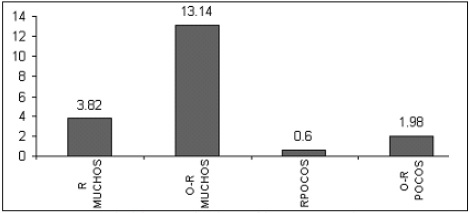
\includegraphics [scale=0.95]{capitulo4/images/grafico1.jpg}
  \end{center}
 \caption[Tasa de bloques leidos para GROUP BY sencillo]{\label{grafico1}Tasa de bloques leidos a filas procesadas para
GROUP BY sencillo \cite{comparacion}}
 \end{figure}
%%%%%%%%%%%%%%%%%%

%%%%%%%%%%%%%%%%%%%%
\begin{figure}[H]
 \begin{center}
  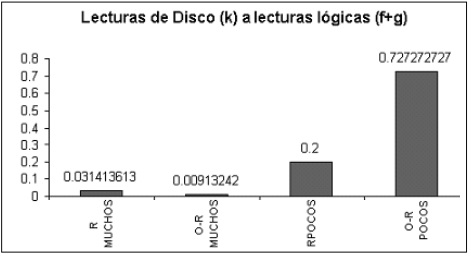
\includegraphics [scale=0.95]{capitulo4/images/grafico2.jpg}
  \end{center}
 \caption[Tasa de lecturas de disco para GROUP BY sencillo]{\label{grafico2}Tasa de lecturas de disco a lecturas l�gicas para
GROUP BY sencillo \cite{comparacion}}
 \end{figure}
%%%%%%%%%%%%%%%%%%%

\noindent En consultas del tipo GROUP BY con las
cl�usulas HAVING y ORDER BY, en la tasa de bloques le�dos a filas
procesadas, se observa en la figura \ref{grafico3} nuevamente la
ventaja que posee el modelo relacional con respecto al modelo objeto relacional
especialmente cuando se ejecuta sobre muchos datos. De forma contraria, en la
tasa de lecturas de disco a lecturas l�gicas, se observa en la figura
\ref{grafico4} un comportamiento pobre en el modelo relacional, y muestra ser un
modelo excesivamente costoso (para este caso) comparado con el
modelo objeto relacional, el cual presenta valores bastante
eficientes.


%%%%%%%%%%%%%%%%%%%%
\begin{figure}[H]
 \begin{center}
  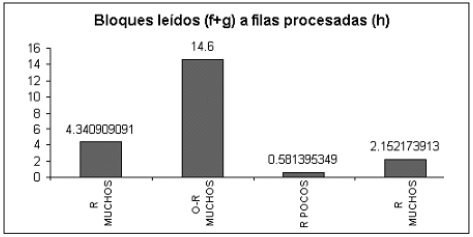
\includegraphics [scale=0.95]{capitulo4/images/grafico3.jpg}
  \end{center}
 \caption[Tasa de bloques le�dos para GROUP BY HAVING y ORDER BY]{\label{grafico3}Tasa de bloques le�dos a filas procesadas para
GROUP BY con las cl�usulas HAVING y ORDER BY \cite{comparacion}}
 \end{figure}
%%%%%%%%%%%%%%%%%%%

%%%%%%%%%%%%%%%%%%%
\begin{figure}[H]
 \begin{center}
  \includegraphics [scale=0.95]{capitulo4/images/grafico4.jpg}
  \end{center}
 \caption[Tasa de lecturas de disco en GROUP BY HAVING y ORDER
 BY]{\label{grafico4}Tasa de lecturas de disco a lecturas l�gicas para GROUP BY con las cl�usulas HAVING y ORDER BY \cite{comparacion}}
 \end{figure}
%%%%%%%%%%%%%%%%%%

\noindent Para las consultas que utilizan subconsultas, fueron probadas
aquellas que se realizan con las cl�usulas IN y EXISTS.
Primero se mostrar�n los resultados con las subconsultas
cuando se utiliza la cl�usula EXISTS, y luego los resultados
cuando se utiliza la cl�usula IN. En el primer caso se puede observar en la
figura \ref{grafico5} que en la tasa de bloques le�dos a filas procesadas,
existe una diferencia bastante significativa entre ambos modelos donde se
visualiza una ganancia bastante visible del modelo relacional sobre el modelo
objeto relacional, que en este caso muestra una eficiencia baja. 
De manera an�loga a las pruebas realizadas sobre las subconsultas cuando se
utiliza la cl�usula EXISTS, las pruebas con la cl�usula IN cuyos
resultados son presentados en la figura
\ref{grafico6}, muestran que en la tasa de bloques le�dos a filas procesadas el
modelo relacional ofrece de nuevo un rendimiento superior con respecto
al modelo objeto relacional. Adem�s de acuerdo con los resultados
que, aunque la cl�usula EXISTS deber�a ser m�s eficiente
que la cl�usula IN \cite{oratunning}, en
este caso particular los dos tipos de subconsultas ofrecen un rendimiento
exactamente igual. En las dem�s tasas, en ambos casos, los dos modelos se
comportaron de manera eficiente.

%%%%%%%%%%%%%%%%%%%
\begin{figure}[H]
 \begin{center}
  \includegraphics [scale=0.95]{capitulo4/images/grafico5.jpg}
  \end{center}
 \caption[Tasa de bloques le�dos para las subconsultas con EXISTS]{\label{grafico5}Tasa de bloques le�dos a filas procesadas para las subconsultas cuando se utiliza la cl�usula EXISTS \cite{comparacion}}
 \end{figure}
%%%%%%%%%%%%%%%%%%%

%%%%%%%%%%%%%%%%%%%%
\begin{figure}[H]
 \begin{center}
  \includegraphics [scale=0.95]{capitulo4/images/grafico6.jpg}
  \end{center}
 \caption[Tasa de bloques le�dos para las subconsultas con la cl�usula
 IN]{\label{grafico6}Tasa de bloques le�dos a filas procesadas para las subconsultas cuando se utiliza la cl�usula IN \cite{comparacion}}
 \end{figure}
%%%%%%%%%%%%%%%%%%%
\chapter{Mapeo objeto relacional (ORM)}\label{orm}

\par \noindent Para poder acceder a una base de datos relacional desde
una aplicaci�n que haya sido desarrollada basada en los principios de la
programaci�n orientada a los objetos, se requiere de una interfaz que
permita traducir representaciones de datos de los sistemas de bases
de datos relacionales, a representaciones de objetos, a esta interfaz se le
denomina mapeo objeto-relacional (ORM, Object-Relational Mapping). Como los sistema de
administraci�n de base de datos relacionales no poseen la flexibilidad para 
representar datos no escalares, como lo son arreglos y s�lo soportan tipos de datos simples, 
haci�ndose preciso la conversi�n de los objetos en un conjunto de valores simples, y viceversa, 
de manera que el objeto, sus propiedades y relaciones puedan ser recuperados.

\noindent La existencia de un ORM es primordial para el desarrollo de sistemas
de software robustos y escalables. T�picamente los desarrolladores son quienes deb�an
escribir el c�digo asociado a la persistencia de la informaci�n, de forma que
dicha informaci�n pudiera ser almacenada en las tablas de la base de datos. 

\par \noindent Un principio universal en la mayor�a de las aplicaciones es la
independencia de los datos, teniendo en cuenta el gran n�mero de ventajas que
esto proporciona. Este principio propone que una base de datos debe ser
administrada y mantenida de manera independiente de cualquier programa que haga
uso de ella. No obstante, en el proceso de construcci�n de software esta
independencia de datos ocasiona ciertos efectos negativos para los
desarrolladores. Esto es debido a la mezcla de dos lenguajes incompatibles, como
lo son el lenguaje de consulta para almacenar y recuperar los datos, y adem�s el
lenguaje de programaci�n que deja a los usuarios interactuar con las bases de
datos desde la aplicaci�n. Entre estos dos modelos existe una brecha denominada
desajuste por impedancia \cite{subieta}, dada por las diferencias entre uno y
otro. Una de las principales diferencias se debe a que en los sistemas de bases
de datos relacionales, los datos siempre son manejados en forma de tablas,
constituidas por un conjunto de filas o tuplas; mientras que en los entornos
orientados a objetos los datos son manipulados como objetos, formados a su vez por objetos y tipos elementales.

\noindent Para disminuir los efectos del desajuste de impedancia entre ambos modelos, existen pr�cticas y t�cnicas como:

\begin{itemize}
  \item Objetos de acceso a datos (Data Acces Objects o DAOs).
  \item Frameworks de persistencia (Persistence Frameworks).
  \item Mapeadores objeto relacionales (Object relational mappers u ORM).
  \item Consultas nativas (Native queries).
  \item Lenguajes integrados como: PL/SQL (Oracle) y T-SQL(SQLServer).
  \item Mediadores.
  \item Repositorios virtuales.
  \item Bases de datos orientadas al objeto.
\end{itemize}

\par \noindent A continuaci�n se dar� un mayor detalle en los tipos de
mapeadores y los frameworks de persistencia, ya que son los conceptos m�s
relevantes para el presente estudio.

\section{Tipos de mapeadores}

\par \noindent Se presentar�n los tipos b�sicos de mapeadores por dise�o de
originado por entidades de negocio. Se comenzar� por un enfoque simple que es
utilizado en aplicaciones muy simples tales como un libro de visitas en p�ginas
de internet.

\subsection{Enfoque a tuplas}

\par \noindent Cuando este enfoque es utilizado, es una pregunta v�lida si es
que realmente se est� hablando sobre mapeo objeto relacional, ya que las
aplicaciones simplemente leen registros desde el SADB a un record set y luego
trabajan con dichos record sets. Los datos no son le�dos como objetos (entidades
de negocio).
Este enfoque no es apropiado para el desarrollo de sistemas de gran envergadura,
porque la l�gica de negocios se encuentra estrechamente unida con el formato de
los datos en el almac�n de datos. Cuando por ejemplo un atributo se mueve de una
tabla a otra (por refactorizaci�n), todos los lugares en el c�digo fuente de la
aplicaci�n, que trabajen con este atributo deben ser cambiados.

\subsection{Enfoque a entidades}

\par \noindent Como en el caso anterior, la aplicaci�n lee datos a un record set
en primera instancia. Luego de leer a un record set, las entidades de negocios
son llenadas con los datos del record set. Estas entidades de negocio tienen
forma de estructuras de datos, las cuales son muy similares a las tablas de una
base de datos relacional. Por ejemplo en ADO.NET se utilizan \ti{DataSets} o
\ti{DataTables}. De hecho una \ti{DataTable} de ADO.NET es una estructura
tabular, la cual puede tener restricciones definidas como PK o FK. Por otro lado
un \ti{DataSet} es un conjunto de \ti{DataTables}, entre los cuales se pueden
definir relaciones, adem�s posee soporte para actualizaci�n o eliminaci�n en
cascada. La desventaja de este enfoque se centra en que las entidades de
negocios no poseen m�todos, no tienen ning�n comportamiento. S�lo se pueden
observar m�todos simples asociados con el procesamiento de bajo nivel de
datos. %Existen m�todos como \ti{CheckConstraints()}.
\noindent La l�gica de negocio est� ubicada en lo que es llamado clases
de gesti�n. Este tipo de dise�o preserva el pensamiento relacional al nivel de
objetos.

\subsection{Enfoque a modelo de dominio}

\par \noindent Este enfoque es similar al enfoque a entidades, la diferencia
est� en las entidades de negocio. En este enfoque las entidades de negocios son
objetos reales con comportamiento. Los objetos no s�lo son contenedores para
im�genes de tablas de bases de datos. Se puede utilizar herencia, poliformismo y
otros conceptos de la orientaci�n al objeto. La l�gica de negocio est� ubicada
en los m�todos de las entidades de negocio. No existe necesidad de clases de
gesti�n, tal como se mencion� anteriormente.

\section{Frameworks de persistencia}

\par \noindent La mayor�a de las herramientas emplea un mapeo entre el mundo
relacional y el mundo orientado a objetos. En este mapeo se declara como la
herramienta que debe materializar o serializar el objeto desde o hacia la base
de datos. Las herramientas normalmente tambi�n implementan un pseudo lenguaje 
para hacer consultas sobre los datos, este lenguaje es normalmente basado 
en objetos en vez de tablas y sus relaciones, la herramienta traduce 
despu�s al SQL nativo de la base de datos. Muchas herramientas ORM 
tambi�n manejan conceptos como cache, connection pooling, entre otros. Las
herramientas ORM tratan de esconder el mundo relacional 
al desarrollador para que el pueda poner sus esfuerzos en la l�gica de la
aplicaci�n.
\par \noindent Utilizando herramientas ORM se acelera el proceso de desarrollo
de software. Adem�s se obtiene una independencia del motor de base de datos ya
que el desarrollador no escribe SQL directamente sino que un pseudo leguaje que
es traducido al SQL espec�fico de la base de datos configurada.
\noindent Por otro lado la traducci�n adicional es un paso extra que toma m�s
tiempo y por lo cual en algunos casos, especialmente reportes, el redimiendo de
las consultas puede disminuir.
Muchas bases de datos optimizan sus consultas y pueden mejorar los tiempos de
respuesta al emplease procedimientos almacenados, al generar SQL en ejecuci�n se
pierde esta oportunidad de optimizaci�n. Algunas herramientas ORM no optimizan la consulta para la base de datos 
utilizada, sino que generan un SQL gen�rico lo cual resulta en una muy mala

\noindent Existen diversas herramientas que realizan la transformaci�n seg�n el
lenguaje de programaci�n y el motor de base de datos, en la tabla \ref{tabla22} se muestran los productos
de software ORM m�s destacados de la actualidad.

 \begin{table}[H]
  \begin{center}
 \begin{tabular}{|p{5cm}|l|p{3.5cm}|}
    \hline
    \tn{Software} & \tn{Plataforma} & \tn{Disponibilidad}  \\ \hline 
    Dapper     & .NET 4.0        & Open source   \\ \hline
    ECO		&	.NET 4.0 		&	Comercial	\\ \hline
    EntitySpaces	&	.NET 4.0 	& Open source \\ \hline
    EclipseLink		&	Java Virtual Machine	&	Open source \\ \hline
   	Hibernate 	&	Java Virtual Machine &	Open source \\ \hline
   	iBATIS		&	Multiplataforma		&	Open source	 \\ \hline
   	LLBLGen\_Pro		&	.NET 4.0	&	Comercial\\ \hline
   	Microsoft ADO.NET Entity Framework	& .NET 4.5 	& Parte de .NET 4.5\\	\hline
   	nHibernate		& .NET 4.0	&	Open source\\	\hline
   	ODB		&	Multiplataforma C++		&	Licencia dual\\	\hline
   	SQLAlchemy	&	Python	&	Open source\\	\hline
   	SQLObject	&	Python	&	\\	\hline
   	Storm		&	Python	&	Open source\\	\hline
   	SubSonic	&	.NET 2.0	&	Open source	\\	\hline
   	TopLink		&	Java Virtual Machine	&	Comercial\\	\hline
   	WebORB Integration Server	&	.NET, Java, PHP		&	Open source \& comercial\\
   	\hline
    \end{tabular}
    \caption{\label{tabla22}Herramientas ORM populares en la actualidad}
    \end{center}
\end{table}

\end{appendices}
% %\appendix
% %\addcontentsline{toc}{chapter}{Apendice}
% %\setcounter{chapter}{0}
% %\renewcommand{\chaptername}{{\huge\bfseries APENDICE}}
% %\renewcommand{\thechapter}{\Alph{chapter}}
% %\renewcommand{\thesection}{\Alph{chapter}.\arabic{section}}
% %\renewcommand{\thefigure}{\Alph{chapter}.\arabic{figure}}
% 
% \addcontentsline{toc}{chapter}{Ap�ndice A: Algoritmos Gen�ticos (AG)}
% \include{apendices/apendiceAG}
% 
% \addcontentsline{toc}{chapter}{Ap�ndice B: Configuraci�n}
% \include{apendices/apendiceConfiguracion}
% 
% \addcontentsline{toc}{chapter}{Ap�ndice C: C�digo Programas de Prueba}
% \include{apendices/apendiceTest}
% 
% \addcontentsline{toc}{chapter}{Ap�ndice D: C�digo Base}
% \include{apendices/apendiceCodigoBase}
% 
% \addcontentsline{toc}{chapter}{Ap�ndice E: C�digo Estrategias}
% \include{apendices/apendiceCodigoEstrategias}



%\include{apendiceCod}
% \def\bibname{Referencias}


%\addcontentsline{toc}{chapter}{Referencias}

\end{document}
